\documentclass[12pt]{article}

%% Packages
\usepackage[margin=1in, top=0.75in]{geometry}
\usepackage[utf8]{inputenc}
\usepackage[T1]{fontenc}
\usepackage[usenames,dvipsnames]{xcolor}
\usepackage{amssymb, amsfonts, amsmath, mathrsfs, enumitem, tcolorbox, bbm, graphicx, fullpage, parskip, mathtools, float, amsthm}
\usepackage{tikz,sgame,bbm,todonotes, setspace, soul, array}
\usepackage[english]{babel}
\usepackage{pdfpages}
\setcounter{tocdepth}{3}
% Links (and references)
\definecolor{linkblue}{RGB}{40, 50, 200}
\usepackage[colorlinks=true, allcolors={linkblue}]{hyperref}

%% Math operators
\newcommand*{\ones}{\text{\usefont{U}{bbold}{m}{n}1}}
\newcommand{\reals}{\mathbb{R}}
\newcommand{\rationals}{\mathbb{Q}}
\newcommand{\integers}{\mathbb{Z}}
\newcommand{\naturals}{\mathbb{N}}
\newcommand{\complex}{\mathbb{C}}
\newcommand{\normal}{\mathcal{N}}

% General math
\newcommand{\abs}[1]{\mathop{\left|#1\right|}} % absolute value
\newcommand{\inv}{^{-1}} % inverse
\let\oldST\st
\newcommand{\strikethrough}{\oldST}
\renewcommand{\st}{\;\text{s.t.}\;} % math operator for "such that"
\newcommand{\eg}{\emph{e.g.} }
\newcommand{\ie}{\emph{i.e.} }
\newcommand{\interior}{\mathop{\rm int}}

% Optimization
\newcommand{\argmax}{\mathop{\rm argmax}}
\newcommand{\argmin}{\mathop{\rm argmin}}
\newcommand{\opt}{^\star}
% Analysis, vector spaces, and topology
\newcommand{\set}[1]{\left\{#1\right\}} % set notation
\newcommand{\seq}[1]{_{#1}^{\infty}} % add sequence notiation to set (or to a summation symbol for series)
\newcommand{\setless}{\mathop{\backslash}} % A \ B notation
\newcommand{\pow}{\mathop{\mathcal{P}}} % power set
\newcommand{\im}{\mathop{\rm im}} % image
\newcommand{\spans}{\mathop{\rm span}} % span
\newcommand{\rank}{\mathop{\rm rank}} % rank
\newcommand{\topo}{\mathop{\mathcal{T}}} % topology
\newcommand{\cont}{\mathop{\bf C}} % continuously differentiable

% Matrices
\newcommand\colvector[1]{\begin{bmatrix}#1\end{bmatrix}}
\newcommand\rowvector[1]{\begin{bmatrix}#1\end{bmatrix}}
\newcommand\matrixc[1]{\begin{bmatrix}#1\end{bmatrix}}
\newcommand\matrixp[1]{\begin{pmatrix}#1\end{pmatrix}}
\newcommand\detmatrix[1]{\begin{vmatrix}#1\end{vmatrix}}
\newcommand\rankmatrix{\begin{bmatrix}I_r & \rvline & \mathbf{0}_1\\\hline \mathbf{0}_2 & \rvline & \mathbf{0}_3 \end{bmatrix}}

% Statistics
\newcommand{\cov}{\mathop{\rm cov}} % covariance
\newcommand{\corr}{\mathop{\rm corr}} % correlation
\newcommand{\expect}{\mathop{\mathbb{E}}} % expectation
\newcommand{\indep}{\perp \hspace{-1.4ex} \perp} % independence symbol
\newcommand{\distiid}{\mathop{\overset{\text{i.i.d.}}\sim}} % i.i.d.
\newcommand{\oversim}[1]{\mathop{\overset{\text{#1}}\sim}} % general text over \sim
\newcommand{\prob}{\mathbb{P}}
\newcommand{\mse}{\mathop{\rm MSE}}
\newcommand{\var}{\mathop{\rm Var}}
\newcommand{\sd}{\mathop{\rm sd}}
\newcommand{\se}{\mathop{\rm se}}
\newcommand{\bias}{\mathop{\rm bias}}
\newcommand{\toprob}{\overset{p}{\to}}
\newcommand{\toas}{\overset{a.s.}{\to}}
\newcommand{\todist}{\overset{d}{\to}}
\newcommand{\hyp}{\mathbb{H}}

% Economics
\newcommand{\choice}{\mathop{C_{\succsim}}} % choice correspondence

% Update existing operators
\let\oldExists\exists
\renewcommand{\exists}{\oldExists\;}
\let\oldForall\forall
\renewcommand{\forall}{\;\oldForall\;}
\let\oldEmptyset\emptyset
\renewcommand{\emptyset}{\mathop{\varnothing}}
\newcommand{\parl}{\left(}
\newcommand{\parr}{\right)}
\newcommand{\midbar}{\middle|}
\newcommand{\barl}{\left[}
\newcommand{\barr}{\right]}
\newcommand{\curll}{\left\{}
\newcommand{\curlr}{\right\}}


%% Presentation environments
% Proofs, counterexamples, and disproofs
\renewcommand\qedsymbol{$\openbox$}
\renewenvironment{proof}{{\raggedright \textit{\textbf{Proof.}}}}{\qed} % Proof
\newenvironment{pf}{\begin{proof}}{\end{proof}} % Proof (shorthand)

\newenvironment{disproof}{{\raggedright \textit{\textbf{Disproof.}}}}{$\qed$} % Disproof
\newenvironment{counterex}{{\raggedright \textit{\textbf{Counterexample.}}}}{} % Counterexample

% Theorem styles
\theoremstyle{plain}
\newtheorem{result}{Result}
\newtheorem{lemma}{Lemma}[section]

\newtheorem{theorem}{Theorem}[section]
\newtheorem{proposition}{Proposition}[section]
\newtheorem{corollary}{Corollary}[section]
\newtheorem{axiom}{Axiom}[section]
\theoremstyle{definition}
\newtheorem*{example}{Example}
\newtheorem*{definition}{Definition}
\newtheorem*{exercise}{Exercise}
\newtheorem*{model}{Model}
\newtheorem*{proposition*}{Proposition}
\newtheorem*{model*}{Model}
\newtheorem*{solution}{Solution}
\newtheorem*{remark}{Remark}
\newtheorem*{question}{Question}
\newtheorem*{answer}{Answer}
\newtheorem*{algorithm}{Algorithm}
\newtheorem{assumption}{Assumption}[section]

\newcommand{\blue}[1]{\textcolor{blue}{\emph{#1}}}
\newcommand{\red}[1]{\textcolor{red}{\emph{#1}}}




\newcommand{\gabe}[1]{\todo[inline,color=green!20!white]{\textbf{GS:} #1}}


%% Header
\makeatletter
\newcommand{\course}[1]{\def\@course{#1}}
\newcommand{\term}[1]{\def\@term{#1}}
\renewcommand{\title}[1]{\def\@entitle{#1}}
\renewcommand{\maketitle}{
    \begin{tcolorbox}[colframe=darkgray]
        \begin{center}
            \textbf{\@course} \\[0.25em]
            {\Large\textit{\@entitle}} \\[0.5em]
            \@author \\[0.5em]
            \@term
        \end{center}
    \end{tcolorbox}
    \vspace{1em}
}
\makeatother


%% Code
\usepackage{listings}
\usepackage{beramono}
\lstdefinelanguage{Julia}%
  {morekeywords={abstract,break,case,catch,const,continue,do,else,elseif,%
      end,export,false,for,function,immutable,import,importall,if,in,%
      macro,module,otherwise,quote,return,switch,true,try,type,typealias,%
      using,while},%
   sensitive=true,%
   alsoother={$},%
   morecomment=[l]\#,%
   morecomment=[n]{\#=}{=\#},%
   morestring=[s]{"}{"},%
   morestring=[m]{'}{'},%
   breaklines=true,%
}[keywords,comments,strings]%

\lstset{%
    language         = Julia,
    basicstyle       = \ttfamily,
    keywordstyle     = \bfseries\color{blue},
    stringstyle      = \color{magenta},
    commentstyle     = \color{ForestGreen},
    showstringspaces = false,
}






\title{Microeconomics I Notes}
\author{Gabe Sekeres \& Omar And\'{u}jar}
\course{ECON 6090}
\term{Fall 2024}
\begin{document}
\maketitle

\tableofcontents

\newpage

\section*{Introduction}

We are creating this set of unified notes for ECON 6090: Microeconomics I, as taught at Cornell University in the Fall 2024 semester. Due to unforeseen departmental circumstances, this course was taught by six different professors (\href{https://easley.economics.cornell.edu/}{David Easley}, \href{https://philippkircher.com/}{Philipp Kircher}, \href{https://adamharris.phd/}{Adam Harris}, \href{https://sites.santafe.edu/~leb/}{Larry Blume}, \href{https://barseghyan.economics.cornell.edu/}{Levon Barseghyan}, and \href{https://www.mbattaglini.com/}{Marco Battaglini}). This structure necessarily created some confusion in notation and material, so these notes function as my attempt to create a universe of the material we learned.

We rely heavily on the notes created from Prof. Easley's course, which were originally compiled by \href{https://julienneves.com/}{Julien Manuel Neves} and subsequently updated by \href{https://ruqing-xu.github.io/}{Ruqing Xu} and \href{https://economics.cornell.edu/patrick-ferguson}{Patrick Ferguson}, as well as the excellent TA Sections curated by \href{https://economics.cornell.edu/yuxuan-ma}{Yuxuan Ma} and \href{https://dyson.cornell.edu/programs/graduate/graduate-student-directory/}{Feiyu Wang}. We additionally rely on notes and slides provided by Prof. Harris, slides provided by Prof. Blume, slides from \href{https://blogs.cornell.edu/odonoghue/}{Ted O'Donoghue} provided by Prof. Barseghyan, and notes provided by Prof. Battaglini. These notes are supplemented with the canonical \href{https://global.oup.com/academic/product/microeconomic-theory-9780195073409?cc=us&lang=en&}{Microeconomic Theory} textbook by \href{https://www.upf.edu/web/andreu-mas-colell}{Andreu Mas-Colell}, \href{https://mitsloan.mit.edu/faculty/directory/michael-whinston}{Michael Whinston}, and \href{https://www.hbs.edu/faculty/Pages/profile.aspx?facId=6466}{Jerry Green} (hereafter, MWG); \href{https://www.semanticscholar.org/paper/Utility-theory-for-decision-making-Fishburn/905a24a912171436e0abd3b5f1fdcb963e6f852f}{Utility Theory for Decision Making} by \href{https://en.wikipedia.org/wiki/Peter_C._Fishburn}{Peter Fishburn}; a classic analysis textbook, \href{https://store.doverpublications.com/products/9780486477664}{Foundations of Mathematical Analysis} by \href{https://condor.depaul.edu/~rjohnson/}{Richard Johnsonbaugh} and \href{https://www.mathgenealogy.org/id.php?id=12494}{W.E. Pfaffenberger}; and the excellent Mathematics notes provided by \href{https://www.takumahabu.com/Economics}{Takuma Habu}. All mistakes are our own.

We occasionally make reference to the Stanford ECON 202 notes, created by \href{https://www.gsb.stanford.edu/faculty-research/faculty/jonathan-levin}{Jonathan Levin}, \href{https://web.stanford.edu/~isegal/}{Ilya Segal}, \href{https://milgrom.people.stanford.edu/}{Paul Milgrom}, and \href{https://sites.google.com/site/ravijagadeesan/}{Ravi Jagadeesan}. This will mainly be if there exists intuition that we believe is helpful.

Thanks to our cohort for helping with this project, especially Robert Betancourt, and Addie Sutton.

\paragraph{Notation.} A large part of this project is an attempt to unify the notation used by our separate professors. We default to the notation used in the Easley notes, then to MWG, and then use our own judgement. New definitions will have a word highlighted in \blue{blue}, and certain (named) theorems will be denoted in \red{red}. 

\paragraph{Structure.} The course (and these notes) are organized as follows. Prof. Easley taught an introduction to choice theory, Section~\ref{sec:easley}. Prof. Kircher taught consumer theory, Section~\ref{sec:kircher}. Prof. Harris taught producer theory, and some concepts of market failures, Section~\ref{sec:harris}. Prof. Blume introduced the theory of choice under uncertainty, Section~\ref{sec:blume}, and Prof. Barseghyan continued with theoretical applications for uncertainty and expected utility maximization, Section~\ref{sec:barseghyan}. Prof. Battaglini taught on information theory, Section~\ref{sec:battaglini}. We also include here exercises with solutions, divided into the various sections and sources. This is Section~\ref{sec:exercises}.


\newpage
\section{Choice (Easley)}\label{sec:easley}

\subsection{Preference Theory}

\begin{assumption}
	Let $X$ be a finite set of objects. 
\end{assumption}

\begin{definition}
	Define $\succsim$, a \blue{preference relation} on $X$, as $x \succsim y \Longleftrightarrow x$ is \emph{at least as good as} $y$, for $x,y \in X$. $\succsim$ is a binary relation.
\end{definition}

\begin{definition}
	$x$ is \blue{strictly preferred} to $y$, denoted as $x \succ y$, if $x \succsim y$ and $y \not\succsim x$.
\end{definition}
\begin{definition}
	$x$ is \blue{indifferent} to $y$, denoted as $x \sim y$, if $x \succsim y$ and $y \succsim x$.
\end{definition}

\begin{definition}
	A preference relation $\succsim$ is \blue{complete} if $\forall x,y \in X$, either $x\succsim y$, $y \succsim x$, or both.
\end{definition}
\begin{definition}
	A preference relation $\succsim$ is \blue{transitive} if, $\forall x,y,z \in X$ where $x \succsim y$ and $y \succsim z$, $x \succsim z$.
\end{definition}
\begin{definition}
	A preference relation $\succsim$ is \blue{rational} if it is complete and transitive.
\end{definition}
\begin{remark}
	Prof. Easley takes some issues with this definition. The main issue is that there is an English word `rational' that has absolutely nothing to do with it. Hereafter, always read rational as `complete and transitive'.
\end{remark}

\begin{remark}
	These are all of the abstract concepts in choice theory! From here, we will apply them, and see what we can get. 
\end{remark}

\begin{definition}
	(Informal) Define a \blue{choice structure} $C\opt$ over subsets $B \subseteq X$ as $C\opt(B,\succsim) \coloneqq \{x \in B : x \succsim y \forall y \in B\}$.
\end{definition}
\begin{remark}
	Some direct implications:
	\begin{itemize}
		\item[(i)] If $x \in C\opt(B,\succsim)$ and $y \in C\opt(B,\succsim)$, then $x \sim y$.
		
		\item[(ii)] Suppose that $x \in B$, $x \not\in C\opt(B,\succsim)$, and $C\opt(B,\succsim) \ne \emptyset$. Then there exists $y \in B$ such that $y \succ x$. 
	\end{itemize}
\end{remark}

We will now formalize the above.

\begin{definition}
	Let the \blue{power set} of $X$, denoted $\mathcal{P}(X)$, be the set of all subsets of $X$. Note that since $X$ is finite, $\mathcal{P}(X)$ is finite.
\end{definition}

\begin{definition}
	(Formal) A correspondence $C\opt : \mathcal{P}(X) \rightrightarrows X$ is a \blue{choice correspondence} for some (not necessarily complete; not necessarily transitive) preference relation $\succsim$ if $C\opt(B) \subseteq B$ for all $B \subseteq X$.
\end{definition}
\begin{remark}
	This definition is from the Stanford notes -- I find it more intuitive than defining it the other way, but it requires divorcing the choice structure from the preference relation. Some intuition that's helpful for me: Easley's definition starts with the preference relation and then defines the choice correspondence, while Segal's definition starts with the choice correspondence and then applies it to a preference relation. They will (as we will see below) often be equivalent, but it's a subtle distinction. I will denote an arbitrary choice correspondence by $C\opt(\cdot)$ and one connected with a preference relation $\succsim$ by $C\opt(\cdot, \succsim)$.
\end{remark}

\begin{proposition}\label{prop:rational_choice_nonempty}
	If $\succsim$ is a rational preference relation on $X$, then
	\[
	C\opt : \mathcal{P}(X) \setminus \emptyset \to \mathcal{P}(X) \setminus \emptyset 
	\]
	In words, the associated choice correspondence to a rational preference relation is nonempty for nonempty inputs.
\end{proposition}
\begin{remark}
	The Easley notes define power sets slightly differently. This is unnecessary and (I feel) less intuitive.
\end{remark}
\begin{proof}
	Proof by induction on $n = |B|$. Suppose $|B| = 1$, so $B = \{x\}$ for some $x \in X$. Then by completeness, $x \succsim x$, and $C\opt(B,\succsim) = \{x\} \in \mathcal{P}(X) \setminus \emptyset$. Suppose next that for any $Y$ where $|Y| = n$, $C\opt(Y,\succsim)$ is nonempty. Take some arbitrary $B$, where $|B| = n + 1$. Define $B'\coloneqq B \setminus \{x\}$, and let $x'$ be an element of $C\opt(B',\succsim)$, which is nonempty by the inductive hypothesis. By completeness, either $x \succ x'$, $x' \succ x$, or $x \sim x'$. Case by case, we would have that $C\opt(B,\succsim) \in \curll\{x\},C\opt(B',\succsim),C\opt(B',\succsim) \cup \{x\}\curlr \subseteq \mathcal{P}(X)$, by transitivity.
\end{proof}

\begin{definition}
	$C\opt$ satisfies \blue{Sen's $\alpha$}, also known as \blue{independence of irrelevant alternatives}, if $x \in A \subseteq B$ and $x \in C\opt(B,\succsim)$ implies that $x \in C\opt(A,\succsim)$.
\end{definition}
\begin{remark}
	The classical example of a preference relation that violates Sen's $\alpha$ is `choosing the second-cheapest wine.' It should be fairly clear to see why this violates Sen's $\alpha$. Is it a rational preference relation?
\end{remark}

\begin{proposition}\label{prop:rational_alpha}
	If $\succsim$ is a rational preference relation, then $C\opt(\cdot,\succsim)$ satisfies Sen's $\alpha$.
\end{proposition}
\begin{proof}
	The result is trivially true if $A = B$. Suppose that $A \subset B$. Let $x \in C\opt(B,\succsim)$. Then $x \succsim y$ for all $y \in B$. In particular, if $y \in A \subseteq B$, then $x \succsim y$. Thus, $x \in C\opt(A,\succsim)$.
\end{proof}

\begin{definition}
	$C\opt$ satisfies \blue{Sen's $\beta$}, also known as \blue{expansion consistency}, if $x,y \in C\opt(A,\succsim)$, $A \subseteq B$, and $y \in C\opt(B,\succsim)$ implies that $x \in C\opt(B,\succsim)$.
\end{definition}

\begin{remark}
	I couldn't find a classical example violating Sen's $\beta$, but a simple one is as follows: assume that the waiter offers you French or Italian wine. You are indifferent between them, but then they remember that they also have California wine. You say 	`in that case, I'll have the French wine'. Again, this directly violate's Sen's $\beta$, but is it rational? Why or why not?
\end{remark}

\begin{proposition}\label{prop:rational_beta}
	If $\succsim$ is a rational preference relation, then $C\opt(\cdot,\succsim)$ satisfies Sen's $\beta$.
\end{proposition}
\begin{proof}
	Let $x,y \in C\opt(A,\succsim)$, $A \subseteq B$, and $y \in C\opt(B,\succsim)$. Since $x \in C\opt(A,\succsim)$, we have $x \succsim y$ since $y \in A$. Since $y \in C\opt(B,\succsim)$, we have $y\succsim z$ for all $z \in B$. By transitivity, $x \succsim y$ and $y \succsim z$ implies that $x \succsim z$ for all $z \in B$, so $x\in C\opt(B,\succsim)$. 
\end{proof}

\begin{definition}
	$C\opt$ satisfies \blue{Houthaker's weak axiom of revealed preference} (often called either \blue{HWARP} or \blue{HARP}) if for all $A,B \in \mathcal{P}(X)$ if $x,y \in A \cap B$, $x \in C\opt(A,\succsim)$ and $y \in C\opt(B,\succsim)$, then $x \in C\opt(B,\succsim)$ and $y \in C\opt(A,\succsim)$.
\end{definition}

\begin{proposition}\label{prop:alpha_beta_hwarp}
	$C\opt : \mathcal{P} \rightrightarrows X$ satisfies Sen's $\alpha$ and $\beta$ if and only if it satisfies Houthaker's weak axiom of revealed preference.
\end{proposition}
\begin{proof}
	
	\begin{itemize}
		\item[(i)] ($\alpha + \beta \Longrightarrow $ HWARP) Suppose $x,y \in A \cap B \subseteq \mathcal{P}(X)$, $x \in C\opt(A,\succsim)$, and $y \in C\opt(B,\succsim)$. By Sen's $\alpha$, both $x$ and $y$ are in $C\opt(A \cap B,\succsim)$. Then by Sen's $\beta$, $x \in C\opt(B,\succsim)$ and $y \in C\opt(A,\succsim)$.
		
		\item[(ii)] (HWARP $\Longrightarrow \beta$) Say $x,y \in C\opt(A,\succsim)$, $A \subseteq B$ and $y \in C\opt(B,\succsim)$. Because $A = A \cap B$, $x,y \in C\opt(A \cap B,\succsim)$. Applying HWARP, we have that $x \in C\opt(B,\succsim)$.
		
		\item[(iii)] (HWARP $\Longrightarrow \alpha$) Say $x \in A \subseteq B$ and $x \in C\opt(B,\succsim)$. Suppose $x \not\in C\opt(A,\succsim)$. Then by Proposition~\ref{prop:rational_choice_nonempty}, there exists $y \in C\opt(A,\succsim)$. Note that $x,y \in A = A \cap B$, $x \in C\opt(B,\succsim)$ and $y \in C\opt(A,\succsim)$. By HWARP, $x \in C\opt(A,\succsim)$, which is a contradiction.
	\end{itemize}
\end{proof}

\begin{proposition}\label{prop:hwarp_alpha_beta_equiv}
	The following are equivalent for $C\opt(\cdot,\succsim)$, where $C\opt: \mathcal{P}(X) \to \mathcal{P}(X)$
	\begin{itemize}
		\item[(i)] $\succsim$ is rational
		\item[(ii)] $C\opt$ satisfies Sen's $\alpha$ and $\beta$
		\item[(iii)] $C\opt$ satisfies HWARP
	\end{itemize}
\end{proposition}
\begin{proof}
	(ii) and (iii) are equivalent by Proposition~\ref{prop:alpha_beta_hwarp}. (i) $\Longrightarrow$ (ii) is given by Propositions~\ref{prop:rational_alpha} and \ref{prop:rational_beta}. Finally, (iii) $\Longrightarrow$ (i) is given below, in the proof of Proposition~\ref{prop:warp_rationality}.
\end{proof}

\subsection{Observed Choice}

Recall the formal definition of choice correspondences above. We will now add some more structure to that definition.

\begin{definition}
	For $\mathcal{B}$ a collection of subsets of $X$, $(\mathcal{B},C)$ is called a \blue{choice structure} if $C(B) \subseteq B$ and $C(B) = \emptyset \Longleftrightarrow B = \emptyset$ for all $B \in \mathcal{B}$.
\end{definition}

\begin{definition}
	The choice structure $(\mathcal{B},C)$ satisfies the \blue{weak axiom of revealed preference} (\blue{WARP}) if for all $A,B \in \mathcal{B}$ where $x$ and $y$ are in both $A$ and $B$, $x \in C(A)$, and $y\in C(B)$, then $x \in C(B)$ and $y \in C(A)$.\footnote{Note the difference in wording from before -- we cannot have as a condition that $x,y \in A \cap B$ as $A \cap B$ is not necessarily in $\mathcal{B}$.}
\end{definition}
\begin{remark}
	When $\mathcal{B} = \mathcal{P}(X)$, WARP is the same as HWARP.
\end{remark}
\begin{definition}
	Given a choice structure $(\mathcal{B},C)$, the \blue{revealed preference relation} $\succsim\opt$ is defined such that $x \succsim\opt y$ if $\exists B \in \mathcal{B}$ such that $x,y \in B$ and $x \in C(B)$.
\end{definition}
\begin{proposition}\label{prop:warp_rationality}
	Suppose that $X$ is finite and $\mathcal{B} = \mathcal{P}(X)$. If $(\mathcal{B},C)$ satisfies WARP then the revealed preference relation that it induces, $\succsim\opt$ is rational and $C(B) = C\opt(B,\succsim\opt)$ for all $B \in \mathcal{B}$.
\end{proposition}
\begin{proof}
	If $\mathcal{B} = \mathcal{P}(X)$ and $(\mathcal{B},C)$ is a choice structure, then $C(Y)$ is defined as nonempty for every $Y = \{x,y\} \subseteq X$. This implies that $x \succsim\opt y$ or $y \succsim\opt x$ for all $x,y \in X$, so $\succsim\opt$ is complete.
	
	Suppose $x\succsim\opt y$ and $y \succsim\opt z$. Then there exists $A \subseteq X$ containing $x$ and $y$ such that $x \in C(A)$; and $B\subseteq X$ containing $y$ and $z$ such that $y \in C(B)$. Moreover, $\{x,y,z\} \subseteq \mathcal{B}$ and $C(\{x,y,z\})$ is nonempty. Suppose $y \in C(\{x,y,z\})$. Then by WARP, $x \in C(\{x,y,z\})$. Suppose $z \in C(\{x,y,z\})$. Then again by WARP, $y \in C(\{x,y,z\})$ and thus $x \in C(\{x,y,z\})$. In any case, $x \in C(\{x,y,z\})$ implies that $x \succsim\opt z$, so $\succsim\opt$ is transitive.
	
	Let $x$ be an element of $C\opt(B,\succsim\opt)$. Then $x \succsim\opt y \forall y \in B$. Since $C(B)$ is nonempty, we have that $z \in C(B)$ for some $z$. By $x \succsim\opt z$, there exists $A \in \mathcal{B}$ such that $x,z \in A$ and $x \in C(A)$. Therefore by WARP, $x \in C(B)$. Conversely, suppose $x \in C(B)$. Then $x \succsim\opt y$ for all $y \in B$, and so $x \in C\opt(B,\succsim\opt)$.
\end{proof}

\begin{remark}
	A stronger version of Proposition~\ref{prop:warp_rationality} exists, though we do not present the proof here:
\end{remark}
\begin{proposition}\label{prop:warp_rationality_3}
	Suppose that $X$ is finite and for all $Y \subseteq X$ where $|Y| \le 3$, $Y \in \mathcal{B}$. If $(\mathcal{B},C)$ satisfies WARP then the revealed preference relation that it induces, $\succsim\opt$ is rational and $C(B) = C\opt(B,\succsim\opt)$ for all $B \in \mathcal{B}$.
\end{proposition}

\begin{remark}
	This does not hold for anything less strong than 3. Consider the following counterexample: Suppose $X = \{x,y,z,w\}$ and $\mathcal{B} = \{\{x,y\},\{y,z\},\{z,w\},\{w,x\}\}$. Let $C$ be defined by:
	\[
	C(\{x,y\}) = \{x,y\} \quad ;\quad C(\{y,z\}) = \{y,z\} \quad ;\quad C(\{z,w\}) = \{z,w\} \quad ;\quad C(\{w,z\}) = \{x\} 
	\]
	Because no pair of elements of $X$ are both in two elements of $\mathcal{B}$, WARP is vacuously satisfied. But neither $x \succsim\opt z$ or $z \succsim\opt x$, so $\succsim\opt$ is incomplete. We can also show that it is intransitive (how?). Moreover, if we extend $C$ to the family of all two-element subsets of $X$, such that everything except for $\{w,x\}$ is mapped to itself (and $C(\{w,z\}) = \{x\}$), $\succsim\opt$ is complete but remains intransitive.
\end{remark}

\subsection{Incomplete Preferences}

\begin{definition}
	$\succ$ is a \blue{strict partial order} if (i) for any $x,y \in X$, if $x \succ y$, then $y \not\succ x$, and (ii) $\succ$ is transitive.
\end{definition}
\begin{remark}
	Note that we are explicitly not defining $\sim$ as $x \sim y$ if $x \not\succ y$ and $y \not\succ x$. The two elements could be incomparable, we do not assume completeness here.
\end{remark}

\begin{proposition}\label{prop:partial_order}
	Define choice by
	\[
	C\opt(A,\succ) \coloneqq \{x \in A : \forall y \in A, y\not\succ x\}
	\]
	where $\succ$ is a strict partial order. Then $C$ satisfies Sen's $\alpha$ but not Sen's $\beta$.
\end{proposition}
\begin{proof}
	
	\begin{itemize}
		\item[(i)] Suppose $x \in A \subseteq B$ and $x \in C(B,\succ)$. Then there does not exist $y \in B$ such that $y \succ x$. It follows that no such $y$ exists in $A \subseteq B$ either, so $x \in C(A,\succ)$.
		
		\item[(ii)] Suppose that $x,y \in C(A,\succ)$, $A \subseteq B$, $y \in C(B,\succ)$, and there is some $z \succ x$ in $B$ such that $y$ and $z$ are incomparable. Then the hypotheses of Sen's $\beta$ are satisfied, but $x \not\in C(B,\succ)$.
	\end{itemize}
\end{proof}

\subsection{WARP and the Slutsky Matrix}

We will make the following assumptions throughout:

\begin{assumption}\label{ass:consumer_struc}
	We have (i) $L$ commodities, $x \coloneqq (x_1,\dots,x_L) \in \reals^L_+$; (ii) prices $p \coloneqq (p_1,\dots,p_L) \in \reals^L_{++}$; (iii) wealth $w > 0$; and (iv) budget set $B_{p,w} \coloneqq \{x \in \reals^L_+ : p\cdot x \le w\}$.
\end{assumption}

\begin{definition}
	We define the \blue{Walrasian demand function} (also sometimes called the \blue{Marshallian demand function}) by $x : \reals^L_{++} \times \reals_{++} \to \reals^L_+$, where $x(p,w)$ is the consumer's choice at prices $p$ and wealth $w$. Note that $(p,w)$ may not uniquely specify a value. In that case, we have the \blue{Walrasian (Marshallian) demand correspondence}, $X: \reals^L_{++} \times \reals_{++} \rightrightarrows \reals^L_+$.
\end{definition}

\begin{assumption}\label{ass:demand_assumptions}
We will almost always make the following assumptions on $x$:
\begin{itemize}
	\item[(i)] $x(p,w)$ is homogeneous of degree 0, meaning that
	\[
	x(\alpha p ,\alpha w) = x(p,w) \text{ for all } (p,w) \in \reals^L_{++} \times \reals_{++} \text{ and } \alpha > 0
	\]
	\item[(ii)] $x(p,w)$ satisfies Walras' Law: $p \cdot x(p,w) = w$ for all $(p,w) \in \reals^L_{++} \times \reals_{++}$
\end{itemize}
\end{assumption}
\begin{proposition}\label{prop:walras_law_choice_structure}
	Let $\mathcal{B}^W \coloneqq \{B_{p,w} : (p,w) \in \reals^L_{++} \times \reals_{++}\}$ and $C_x(B_{p,w}) \coloneqq \{x(p,w)\}$, and let $x$ be homogeneous of degree 0 and satisfy Walras' Law. Then $(\mathcal{B}^W,C_x)$ is a choice structure.
\end{proposition}
\begin{proof}
	We want to show that $C_x(B_{p,w})$ is a uniquely-defined nonempty subset of $B_{p,w}$ for all $B_{p,w} \in \mathcal{B}^W$. That $C_x(B_{p,w})$ is nonempty follows from the definition of $x$ as a function (or correspondence). Homogeneity of degree 0 implies that for $B_{p,w} = B_{\alpha p,\alpha w}$, $C_x(B_{p,w}) = C_x(B_{\alpha p,\alpha w})$. Walras' Law implies that $C_x(B_{p,w}) \subseteq B_{p,w}$.
\end{proof}

\begin{definition}
	In the context of consumer choice, $x(p,w)$ satisfies the \blue{weak axiom of revealed preferences} (\blue{WARP}) if the following holds: If $(p,w),(p',w') \in \reals^L_{++} \times \reals_{++}$ are such that $p' \cdot x(p,w) \le w'$ and $x(p',w') \ne x(p,w)$, then $p\cdot x(p',w') > w$.
\end{definition}
\begin{remark}
	Basically, if the consumer ever chooses $x'$ when $x$ is available, then there's no way that both $x$ and $x'$ could be available and $x$ would be chosen.
\end{remark}
\begin{definition}
	A \blue{Slutsky compensated price change} is a price change from $p$ to $p'$ accompanied by a change in wealth from $w$ to $w'$ that makes the old bundle just affordable. That is, such that $p' \cdot x(p,w) = w'$.
\end{definition}

\begin{proposition}
	\red{(Law of Compensated Demand)} Suppose that consumer demand $x(p,w)$ is homogeneous of degree 0 and satisfies Walras' Law. Then $x(p,w)$ satisfies WARP if and only if for any compensated price change from $(p,w)$ to $(p',w') \coloneqq (p',p' \cdot x(p,w))$ we have
	\[
	(p' - p)\cdot (x(p',w') - x(p,w)) \le 0
	\] 
	with strict inequality if $x(p',w') \ne x(p,w)$.
\end{proposition}
\begin{proof}
	By WARP, $p \cdot x(p',w') \ge p \cdot x(p,w) = w$, with strict inequality if and only if $x(p,w) \ne x(p',w')$. By Walras' Law, we have that $p'\cdot x(p',w') = p'\cdot x(p,w) = w'$. Subtracting, we get
	\[
	(p - p') \cdot x(p',w') \ge (p - p')\cdot x(p,w) \Longrightarrow (p' - p) \cdot (x(p',w') - x(p,w)) \le 0
	\]
	Conversely, say that $(p' - p) \cdot (x(p',w') - x(p,w)) \le 0$. Then we have that
	\[
	p' \cdot x(p',w') - p' \cdot x(p,w) - p \cdot (x(p',w') - x(p,w)) \le 0 \Longrightarrow p \cdot x(p',w') > w
	\]
	since $p' \cdot x(p',w') < p' \cdot x(p,w)$. The case of strict inequality is analogous.
\end{proof}

\begin{proposition}\label{prop:law_of_demand}
	Let $x : \reals^L_+ \times \reals_+ \to \reals^L_+$ be continuously differentiable. Then
	\[
	\frac{\partial x_j(p,w)}{\partial p_j} + x_j(p,w) \frac{\partial x_j(p,w)}{\partial w} \le 0
	\]
\end{proposition}
\begin{proof}
	Assume that $p$ changes solely in $p_j$, by $\Delta p_j > 0$, and let $\Delta w$ be the compensating change in wealth, as above. Let $\Delta x \coloneqq x(p',w') - x(p,w)$. Then by the Law of Compensated Demand, we have that
	\[
	\Delta p_j (x_j(p',w') - x_j(p,w)) \le 0 \Longrightarrow \frac{x_j(p',w') - x_j(p,w)}{\Delta p_j} \le 0
	\]
	Adding and subtracting $x_j(p',w)$, this becomes
	\[
	\frac{x_j(p',w) - x_j(p,w)}{\delta p_j} + \frac{x_j(p',w') - x_j(p',w)}{\Delta p_j} \le 0
	\]
	Using the fact that $\Delta w = \Delta p_j x_j(p,w)$, we get that
	\[
	\frac{x_j(p',w) - x_j(p,w)}{\delta p_j} + x_j(p,w)\frac{x_j(p',w') - x_j(p',w)}{\Delta w} \le 0
	\]
	Taking the limit as $\Delta p_j \searrow 0$, which implies that $\Delta w \searrow 0$ and $p' \to p$), and using the fact that $x$ is continuously differentiable, this becomes
	\[
	\frac{\partial x_j(p,w)}{\partial p_j} + x_j(p,w) \frac{\partial x_j(p,w)}{\partial w} \le 0
	\]
\end{proof}

\begin{definition}
	The \blue{Slutsky matrix} is the matrix of the partials defined above:
	\begin{align*}
		S(p,w) &\coloneqq D_p x(p,w) + D_w x(p,w) x(p,w)^T \\
		&= \matrixc{\frac{\partial x_1}{\partial p_1} + x_1 \frac{\partial x_1}{\partial w} & \cdots & \frac{\partial x_1}{\partial p_L} + x_L \frac{\partial x_1}{\partial w} \\ \vdots && \vdots \\\frac{\partial x_L}{\partial p_1} + x_1 \frac{\partial x_L}{\partial w} & \cdots & \frac{\partial x_L}{\partial p_L} + x_L \frac{\partial x_L}{\partial w} }
	\end{align*}
\end{definition}

\begin{proposition}\label{prop:slutsky_nsd}
	$S(p,w)$ is negative semi-definite.
\end{proposition}
\begin{proof}
	Let $dp \coloneqq (dp_1,\dots,dp_L)$ be an arbitrary element of $\reals^L$. Then for all $i$, we have that
	\begin{align*}
		dx_i &= \frac{\partial x_i}{\partial p_1}dp_1 + \cdots + \frac{\partial x_i}{\partial p_L}dp_L + \frac{\partial x_i}{\partial w}x_1(p,w)dp_1 + \cdots + \frac{\partial x_i}{\partial w}x_L(p,w)dp_L \\
		\Longrightarrow dx &= (D_px(p,w) + D_wx(p,w) x(p,w)^T) dp
	\end{align*}
	By WARP, $dp \cdot dx \le 0$, meaning that
	\[
	dp^T (D_px(p,w) + D_wx(p,w) x(p,w)^T) dp \le 0
	\]
	Thus, $S(p,w)$ is negative semi-definite, since $dp$ is arbitrary.
\end{proof}


\subsection{Consumer Choice from $\succsim$}

\begin{assumption}
	As before, let $X \coloneqq \reals^L_+$. 
\end{assumption}
\begin{definition}
	A \blue{utility function} representing $\succsim$ on $X$ is a function $u: X \to \reals$ such that for all $x,y \in X$:
	\[
	x \succsim y \Longleftrightarrow u(x) \ge u(y)
	\]
\end{definition}

\begin{proposition}
	If $u: X \to \reals$ represents $\succsim$ on $X$ and $f: \reals \to \reals$ is strictly increasing, then $f \circ u$ represents $\succsim$.
\end{proposition}
\begin{proof}
	\[
	x \succsim y \Longleftrightarrow u(x) \ge u(y) \Longleftrightarrow (f\circ u)(x) \ge (f\circ u)(y)
	\]
\end{proof}

\begin{remark}
	Lexicographic preferences, defined on $\reals^2$ by
	\[
	(x_1,x_2) \succsim (y_1,y_2) \Longleftrightarrow x_1 > y_1 \text{ or } x_1 = y_1 \text{ and } x_2 \ge y_2
	\]
	are rational but cannot be represented by a utility function. Why is that?
\end{remark}

\begin{definition}
	The following mathematical concepts will be useful to us:
	\begin{itemize}
		\item[(i)] The \blue{upper contour set}, $R(x) \coloneqq \{y \in X : y \succsim x\}$, is the set of all bundles that are at least as good as $x$. Denote its complement by $P^{-1}(x)$.
		
		\item[(ii)] The \blue{lower contour set}, $R^{-1}(x) \coloneqq \{y \in X : x \succsim y\}$, is the set of all bundles that $x$ is at least as good as. Denote its complement by $P(x)$.
	\end{itemize}
\end{definition}

\begin{definition}
	The preference relation $\succsim$ on $X$ is \blue{continuous} if $R(x)$ and $R^{-1}(x)$ are closed subsets of $X$ for all $x \in X$.
\end{definition}

\begin{remark}
	Lexicographic preferences are not continuous. Can you show why?
\end{remark}
\begin{proposition}\label{prop:debreu}
	\red{(Debreu's Theorem)} Suppose a preference relation $\succsim$ on $X$ is rational and continuous. Then there is a continuous utility function representing $\succsim$.
\end{proposition}
\begin{proof}
	(Sketch) We will sketch this proof assuming that $\succsim$ satisfy strong monotonicity (defined below), which is not necessary but makes the proof easier. Choose any $x \in X$. By strong monotonicity, $x \succsim 0$. Let $e = (1,1)$. By strong monotonicity, $\exists \alpha \in \reals_+$ such that $\alpha e \succ x$. By strong monotonicity, $\exists \alpha : X \to \reals_+$ such that $\alpha(x)e\sim x \forall x \in X$. 
	
	We claim that $\alpha(\cdot)$ represents $\succsim$. First, suppose that $\alpha(x) \ge \alpha(y)$. Then $\alpha(x)e \succsim \alpha(y)e$ by strict monotonicity, and by transitivity we have that $x \sim \alpha(x)e \succsim \alpha(y)e \sim y \Longrightarrow x \succsim y$. Conversely, assume that $x\succsim y$. Then $\alpha(x)e \sim x \succsim y \sim \alpha(y)e$, so $\alpha(x)e\succsim \alpha(y)e$ by transitivity, and $\alpha(x) \ge \alpha(y)$ by strict monotonicity.
\end{proof}

\begin{definition}
	The preference relation $\succsim$ is \blue{monotone} if for all $x,y \in X$, $x \ge y \Longrightarrow x\succsim y$. It is \blue{strictly monotone} if $x \ge y$ and $x \ne y$ implies that $x \succ y$. Note that the latter implies the former.
\end{definition}

\begin{definition}
	The preference relation $\succsim$ is \blue{locally non-satiated} if for every $x \in X$ and for every $\varepsilon > 0$, there exists $y \in X$ such that $\|x - y\| \le \varepsilon$ and $y \succ x$. Note that strict monotonicity implies local non-satiation.
\end{definition}
\begin{remark}
	We assumed earlier that $X = \reals^L_+$. This concept can be extended to any metric space, replacing the norm with the space's distance function.  
\end{remark}
\begin{definition}
	The preference relation $\succsim$ on $X$ is \blue{convex} if for all $x,y,z\in X$ and all $\alpha \in [0,1]$, $y \succsim x$ and $z \succsim x$ implies that $\alpha y + (1-\alpha)z \succsim x$.
	
	It is \blue{strictly convex} if for all $x,y,z \in X$ and all $\alpha \in (0,1)$, $y \ne z$, $y \succsim x$, and $z \succsim x$ imply that $\alpha y + (1-\alpha)z \succ x$.
\end{definition}

\begin{remark}
	Preferences are convex if and only if $R(x)$ is convex for every $x \in X$. Can you prove this?
\end{remark}

\begin{definition}
	The function $u: X \to \reals$ is \blue{quasiconcave} if for all $x,y \in X$ and any $\alpha \in [0,1]$,
	\[
	u(\alpha x + (1-\alpha)y) \ge \min\{u(x),u(y)\}
	\]
	The function $u: X \to \reals$ is \blue{concave} if for all $x,y \in X$ and any $\alpha \in [0,1]$,
	\[
	u(\alpha x + (1-\alpha)y) \ge \alpha u(x) + (1-\alpha)u(y)
	\]
	Strict quasiconcavity and strict concavity are defined analogously, restricting $\alpha$ to $(0,1)$, requiring that $x \ne y$, and replacing weak inequalities with strict ones.
\end{definition}
\begin{proposition}\label{prop:quasiconcave_convex}
	$u$ representing $\succsim$ is quasiconcave if and only if $\succsim$ is convex.
\end{proposition}
\begin{proof}
	Assuming quasiconcavity, $y,z \succsim z \Longrightarrow u(y),u(z) \ge u(x)$ implies that $u(\alpha y + (1-\alpha)z) \ge \min\{u(y),u(z)\} \ge u(x)$. Conversely, suppose WLOG that $y \succsim z$. Note also that $z \succsim z$. Thus by convexity of preferences, $\alpha y + (1-\alpha)z \succsim z$, meaning that $u(\alpha y + (1-\alpha)z) \ge u(z) = \min\{u(y),u(z)\}$.
\end{proof}

\subsection{Consumer Optimization}

\begin{definition}
	The \blue{consumer's problem} is the optimization problem
	\[
	\max_{x \in \reals^L_+} u(x) \st p \cdot x \le w
	\]
\end{definition}

\begin{proposition}\label{prop:properties_of_x}
	\red{(Properties of Walrasian Demand Correspondence)} Let $u$ be a continuous utility function representing $\succsim$ on $\reals^L_+$.
	\begin{itemize}
		\item[(i)] If $p \in \reals^L_{++}$ and $w \in \reals_{++}$, then there exists an $x\opt \in \reals^L_{++}$ that solves the consumer's problem
		\item[(ii)] If $\lambda > 0$, then $x\opt$ also solves the consumer's problem for $\lambda p$ and $\lambda w$ (homogeneity of degree 0)
		\item[(iii)] If in addition $\succsim$ is locally non-satiated, then Walras' Law holds, meaning that $p \cdot x\opt = w$
		\item[(iv)] If in addition $\succsim$ is strictly convex (equiv. $u$ strictly concave) then $x\opt$ is unique and the Walrasian demand function $x : \reals^L_{++} \times \reals_{++} \to \reals^L_+$ is well-defined and continuous.
	\end{itemize}
\end{proposition}
\begin{proof}
	\begin{itemize}
		\item[(i)] $B_{p,w}$ is nonempty and compact and $u$ is continuous, so conclusion follows from the Extreme Value Theorem.
		
		\item[(ii)] Observe that $p \cdot x \le w \Longleftrightarrow \lambda p \cdot x \le \lambda w$, so the constraint set is the same in both problems.
		
		\item[(iii)] Suppose not: $p \cdot x\opt < w$. Choose $\varepsilon > 0$ such that $p \cdot y < w$ for all $y \in B_\varepsilon(x\opt)$. By local non-satiation, there exists $y \in B_\varepsilon(x\opt)$ such that $y \succ x\opt$. This is a contradiction.
		
		\item[(iv)] Suppose not: let $\hat{x}$ be a distinct solution. Fix $\alpha \in (0,1)$. By strict convexity of preferences, $\alpha \hat{x} + (1-\alpha)x\opt \succ x\opt$. By convexity of the budget set, $\alpha \hat{x} + (1-\alpha)x\opt$ is affordable, contradicting that $x\opt$ is a global maximum. Continuity of $x$ is annoying but proven elsewhere.
	\end{itemize}
\end{proof}

\begin{proposition}\label{prop:necessary_mrs}
	\red{(Necessary Conditions)} Suppose that
	\begin{itemize}
		\item[(i)] The consumer's preferences on $\reals^L_+$ can be represented by a twice continuously differentiable utility function $u$.
		
		\item[(ii)] The preferences are strictly monotone.
		
		\item[(iii)] $p \gg 0$ and $w \gg 0$.
	\end{itemize}
	If $x\opt$ is an interior solution to the consumer's problem (\ie $x\opt \gg 0$), then
	\[
	\text{MRS}_{ij}(x\opt) \coloneqq \frac{\frac{\partial u(x\opt)}{\partial x_i}}{\frac{\partial u(x\opt)}{\partial x_j}} = \frac{p_i}{p_j}
	\]
\end{proposition}
\begin{proof}
	Strict monotonicity implies that $p \cdot x\opt = w$ and $\frac{\partial u(x\opt)}{\partial x_j} > 0$. We know that $x\opt$ solves the consumer's problem, and the constraint qualification holds. By the Karush-Kuhn-Tucker Theorem, there exists $\lambda > 0$ such that $\nabla u(x\opt) = \lambda p$. Conclusion follows.
\end{proof}

\begin{proposition}\label{prop:sufficient_unique}
	\red{(Sufficient Conditions)} Suppose in addition to hypotheses (i) to (iii) of Proposition~\ref{prop:necessary_mrs}, we have 
	\begin{itemize}
		\item[(iv)] $\succsim$ are strictly convex. 
	\end{itemize}
	If $x\opt$ satisfies $x\opt \gg 0$ and $p \cdot x\opt = w$, and there exists $\lambda > 0$ such that $\nabla u(x\opt) = \lambda p$, then $x\opt$ is the unique solution to the consumer's problem.
\end{proposition}
\begin{proof}
	Omitted, but covered in detail in Part 6: Static Optimization of Tak's lecture notes.
\end{proof}

\paragraph{Some Math Remarks.} These last few sections make a number of extremely strong assumptions on the shape and size of $X$. These assumptions are largely not necessary, and can trivially be relaxed as far as assuming that $X$ is a metric space. They can be relaxed significantly further than that, with difficulty. If you are interested in what that entails, I can happily talk for hours about it. If you're not a masochist, you can ignore this entire note and assume we are in non-negative Euclidean space always. - Gabe

\newpage
\section{Consumer Theory (Kircher)}\label{sec:kircher}

\subsection{Utility Maximization}

\begin{remark}
	We will carry forward the assumptions on model structure (Assumptions~\ref{ass:consumer_struc}) made above. We will also generally carry forward Assumptions~\ref{ass:demand_assumptions}, but not as strongly.
\end{remark}

\begin{definition}
	The \blue{indirect utility function}, $V: \reals^L_{++} \times \reals_{++} \to \reals$ is defined by
	\[
	V(p,w) \coloneqq \max_{x \in \reals^L_+} u(x) \st p\cdot x \le w
	\]
\end{definition}
\begin{remark}
	If $x(p,w)$ is a solution to the consumer's problem, then $V(p,w) = u(x(p,w))$. Essentially, if the consumer solves the problem taking into account the constraints, then the value function is their attained utility -- it's how much they get.
\end{remark}
\begin{assumption}\label{ass:consumer_pref_assumptions}
	We assume here that $\succsim$ are locally non-satiated, that $u$ is continuous, and that $p \gg 0$ and $w > 0$.
\end{assumption}

\begin{proposition}
	$V$ has the following properties:
	\begin{itemize}
		\item[(i)] Continuous
		\item[(ii)] Nonincreasing in $p_i$ for $i \in \{1,\dots,L\}$
		\item[(iii)] Strictly increasing in $w$
		\item[(iv)] Quasiconvex, meaning that $\{(p,w) : V(p,w) \le k\}$ is a convex set $\forall k \in \reals$
		\item[(v)] Homogeneous of degree 0
	\end{itemize}
\end{proposition}
\begin{proof}
	
	\begin{itemize}
		\item[(i)] In the case where the solution $x$ is unique, $V = u \circ x$. We assumed continuity of $u$ above, and continuity of $x$ follows from Proposition~\ref{prop:properties_of_x}, as long as $u$ is continuous. A full proof, when $x$ is a correspondence, is omitted but follows from Berge's Theorem.
		\item[(ii)] Fix $i$ and suppose that $p_i' \ge p_i$. Then $B_{p',w} \subseteq B_{p,w}$, so $V(p',w) \le V(p,w)$.
		\item[(iii)] Suppose $w' > w$. Then $p \cdot x(p,w) < w'$, and by local non-satiation there exists $x' \succ x$ such that $p \cdot x' < w'$. Thus, $V(p,w') \ge u(x') > u(x(p,w)) = V(p,w)$.
		\item[(iv)] Fix some $\alpha \in [0,1]$ and some $(p,w),(p',w') \in \reals^L_{++} \times \reals_{++}$, and suppose that
		\[
		x \in B(\alpha p + (1-\alpha)p',\alpha w + (1-\alpha)w')
		\]
		Then we have that
		\[
		\alpha (p \cdot x - w) + (1-\alpha) (p' \cdot x - w') \le 0 \Longrightarrow x \in B_{p,w} \cup B_{p',w'}
		\]
		Meaning that
		\[
		B(\alpha p + (1-\alpha)p',\alpha w + (1-\alpha)w') \subseteq  B_{p,w} \cup B_{p',w'}
		\]
		Which implies that
		\[
		V(\alpha p + (1-\alpha)p',\alpha w + (1-\alpha)w') \le \max\{V(p,w),V(p',w')\}
		\]
		So $V$ is quasiconvex.
		\item[(v)] This follows directly from $x$ being homogeneous of degree 0 (Proposition~\ref{prop:properties_of_x}).
	\end{itemize}
\end{proof}

\begin{proposition}
	If $u$ and $x$ are continuously differentiable, then $V$ is continuously differentiable and
	\[
	\frac{\partial V}{\partial w} = \lambda
	\]
	where $\lambda$ is the Lagrange multiplier in $\mathcal{L}(\lambda,x) = u(x) + \lambda(w-p\cdot x)$.
\end{proposition}
\begin{proof}
	This follows directly from the Envelope Theorem (see Tak's notes for a rigorous definition):
	\[
	\frac{\partial V}{\partial w} = \frac{\partial u}{\partial w} + \lambda
	\]
	and since $u$ is not a function of $w$, the result follows. A more direct proof could also use the chain rule:
	\[
	\frac{\partial V}{\partial w} = \sum_{i=1}^L \frac{\partial u}{\partial x_i}\frac{\partial x_i}{\partial w} = \lambda \sum_{i=1}^L p_i \frac{\partial x_i}{\partial w} = \lambda
	\]
	where the last equality uses Walras' Law, differentiating both sides with respect to $w$.
\end{proof}
\begin{remark}
	We now have some economic intuition for the Lagrange multiplier: it is the marginal utility attained from relaxing the budget constraint by one unit, or the increase in utility from providing the consumer with one more unit of wealth.
\end{remark}


\subsection{Expenditure Minimization}

\begin{definition}
	The \blue{expenditure minimization problem} is the optimization problem
	\[
	\min_{x \in \reals^L_+} p \cdot x \st u(x) \ge \bar{u}
	\]
\end{definition}

\begin{remark}
	$\bar{u}$ is an arbitrary utility level, set as a precondition of the problem. Later, we will see that we usually set $\bar{u}$ as the attained value from the utility maximization problem, but that's actually not necessary for everything here to hold.
\end{remark}

\begin{definition}
	The associated value function, called the \blue{expenditure function}, is defined by
	\[
	e(p,\bar{u}) \coloneqq \min_{x \in \reals^L_+} p \cdot x \st u(x) \ge \bar{u}
	\]
\end{definition}

\begin{definition}
	The \blue{Hicksian demand correspondence}, $H: \reals_{++}^L \times \reals \rightrightarrows \reals_+^L$ gives solutions to the expenditure minimization problem:
	\[
	H(p,\bar{u}) \coloneqq  \argmin_{x \in \reals^L_+} p \cdot x \st u(x) \ge \bar{u}
	\]
	If $H(p,\bar{u})$ is singleton-valued for all $p$ and $\bar{u}$, then we have the \blue{Hicksian demand function} $h: \reals_{++}^L \times \reals \to \reals_+^L$, defined analogously.
\end{definition}

\begin{proposition}\label{prop:hicksian_properties}
	\red{(Properties of Hicksian Demand Correspondence)} Assume that preferences are continuous. Then:
	\begin{itemize}
		\item[(i)] If $u(0) \le \bar{u} \le \sup_{x \in \reals^L_+} u(x)$, where the right hand side is possibly infinite, then there exists $x\opt \in \reals^L_+$ that solves the expenditure minimization problem.
		\item[(ii)] If $\lambda > 0$, then this $x\opt$ also solves the consumer's problem for $\lambda p$ and $\lambda w$ (homogeneity of degree 0).
		\item[(iii)] If $x\opt$ solves the expenditure minimization problem, then $u(x\opt) = \bar{u}$.
		\item[(iv)] If in addition, $\succsim$ is strictly convex then $x\opt$ is unique and the Hicksian demand function $h: \reals_{++}^L \times \reals \to \reals_+^L$ is well-defined and continuous.
	\end{itemize}
\end{proposition}
\begin{proof}
	
	\begin{itemize}
		\item[(i)] By the continuity of $u$ and the Intermediate Value Theorem, there exists $x^0 \in \reals^L_+$ such that $u(x^0) = \bar{u}$. We can then restrict the constraint set without changing the solution to $\{x \in \reals^L_+ : u(x) \ge \bar{u} \text{ and } p \cdot x \le p \cdot x^0\}$. This set is nonempty and compact, so conclusion follows from the Extreme Value Theorem.
		\item[(ii)] This follows directly from the fact that $p \cdot x\opt \ge p \cdot x \Longleftrightarrow \lambda p \cdot x\opt \ge \lambda p \cdot x$.
		\item[(iii)] Suppose FSOC that $u(x\opt) > \bar{u}$. Then by continuity there exists $x \ne x\opt$ such that $x \le x\opt$ and $\bar{u} \le u(x) < u(x\opt)$. Since $p \in \reals^L_{++}$, this implies that $x$ is in the constraint set and attains a lower cost than $x\opt$, contradicting the fact that $x\opt$ is a global minimum.
		\item[(iv)] Suppose FSOC that there exist $x\opt_1$ and $x\opt_2$ both (distinct) global optima, implying that $p \cdot x\opt_1 = p \cdot x\opt_2$. By linearity, this means that taking some $\alpha \in (0,1)$, we have that $p \cdot (\alpha x\opt_1 + (1-\alpha)x\opt_2) = p\cdot x\opt_1$, but by strict convexity we have that $u(\alpha x\opt_1 + (1-\alpha)x\opt_2) > u(x\opt_1) \ge \bar{u}$, contradicting (iii). Continuity and existence follow from Berge's Theorem.
	\end{itemize}
\end{proof}

\begin{proposition}\label{prop:expend_properties}
	\red{(Properties of $e$)} 
	
	\begin{itemize}
		\item[(i)] Continuous
		\item[(ii)] Nondecreasing in $p_i$ for $i \in \{1,\dots,L\}$
		\item[(iii)] Strictly increasing in $\bar{u}$
		\item[(iv)] Homogeneous of degree 1 in $p$
		\item[(v)] Concave in $p$
	\end{itemize}
\end{proposition}
\begin{proof}
	
	\begin{itemize}
		\item[(i)] Follows directly from Berge's Theorem
		\item[(ii)] Let $p' \ge p$ and $x' \in H(p',\bar{u})$. Then $e(p',\bar{u}) = p' \cdot x' \ge p \cdot x' = e(p,\bar{u})$
		\item[(iii)] Same as the proof of (iv) in Proposition~\ref{prop:hicksian_properties} above. 
		\item[(iv)] Follows directly from $H$ being homogeneous of degree 0
		\item[(v)] Let $p'' \coloneqq \alpha p + (1-\alpha)p'$ for some $\alpha \in [0,1]$, $p,p' \in \reals^L_{++}$, and $x'' \in H(p'',\bar{u})$. Then
		\[
		e(p'',\bar{u}) = p'' \cdot x'' = \alpha p \cdot x'' + (1-\alpha) p' \cdot x'' \ge \alpha e(p,\bar{u}) + (1-\alpha)e(p',\bar{u})
		\]
	\end{itemize}
\end{proof}

\subsection{Welfare}

\begin{remark}
	We will carry Assumptions~\ref{ass:consumer_pref_assumptions} through this section.
\end{remark}

\begin{remark}
	Consider a change in price and income from $(p^0,w^0)$ to $(p^1,w^1)$. We want to know what effect this has on the consumer's welfare. It might be useful to compare $V(p^0,w^0)$ to $V(p^1,w^1)$, but $V$ is dependent on the choice of $u$, which is unique only up to positive affine transformation.
\end{remark}

\begin{remark}
	Note that for fixed $p'$, $e(p',V(p,w))$ is a valid indirect utility function, as it is strictly increasing in $V$. Moreover, it is invariant under positive affine transformation of $u$, meaning that if $V$ and $V'$ are indirect utility functions derived from utility functions $u$ and $u'$ representing the same preference relation, then $e(p',V(p,w)) = e(p',V'(p,w))$.
\end{remark}

\begin{definition}
	A \blue{money metric indirect utility function} is an indirect utility function of the form $e(p',V(p,w))$ for some fixed $p'$.
\end{definition}

\begin{remark}
	Which $p'$ should we choose? Henceforth, we consider only a change in prices, fixing wealth at $w$. Let prices change from $p^0$ to $p^1$. Let $u^0 \coloneqq V(p^0,w)$ and $u^1 \coloneqq V(p^1,w)$. 
\end{remark}

\begin{definition}
	The \blue{compensating variation} is the amount of money $CV$ such that the consumer is indifferent between having $w$ at the old prices and having $w - CV$ at the new prices. Formally,
	\[
	CV(p^0,p^1,w) \coloneqq e(p^1,u^1) - e(p^1,u^0) = w - e(p^1,u^0)
	\]
\end{definition}
\begin{definition}
	The \blue{equivalent variation} is the amount of money $EV$ such that the consumer is indifferent between having $w$ at the new prices and $w + EV$ at the old prices
	\[
	EV(p^0,p^1,w) \coloneqq e(p^0,u^1) - e(p^0,u^0) = e(p^0,u^1) - w
	\]
\end{definition}

\begin{remark}
	Note that each are positive when the price changes make the consumer better off and negative when the price changes make the consumer worse off.
\end{remark}

\begin{remark}
	It can be somewhat difficult to wrap your head around the difference between compensating and equivalent variation. Consider the following example: The government is considering implementing a price floor on wheat, and the relevant consumer likes to bake bread. The government wants the consumer to be indifferent between the price floor being implemented or not, and there are two ways to do that. First, they could implement the price floor and then give the consumer money so that they can purchase the same amount of wheat as before. That's compensating variation -- the consumer is \emph{compensated} for the price change occurring. They could also choose not to implement the price floor, but instead tax the consumer so that they can buy as much wheat under the non-price-floor prices as if the price floor was actually enacted. In both cases, the consumer is indifferent between the price floor being implemented or not (or, indifferent under very strong assumptions on preferences. This is a toy example), but the mechanism is different.
\end{remark}

\begin{proposition}\label{prop:ev_cv}
	Suppose the price of only one good changes. WLOG, let that good have index 1. Then
	\[
	EV(p^0,p^1,w) = \int_{p_1^1}^{p_1^0} h_1(p_1,p_{-1},u^1)dp_1
	\]
	and
	\[
	CV(p^0,p^1,w) = \int_{p_1^1}^{p_1^0} h_1(p_1,p_{-1},u^1)dp_1
	\]
\end{proposition}
\begin{proof}
	We assume that $h_1$ is well-defined and integrable with respect to $p_1$ (this can be proven, but we assume it for simplicity). Then we have that
	\begin{align*}
		EV(p^0,p^1,w) &= e(p^0,u^1) - e(p^0,u^0) = \int_{p_1^1}^{p_1^0} h_1(p_1,p_{-1},u^1)dp_1 \\
		CV(p^0,p^1,w) &= e(p^1,u^1) - e(p^1,u^0) = \int_{p_1^1}^{p_1^0} h_1(p_1,p_{-1},u^1)dp_1
	\end{align*}
\end{proof}

\begin{remark}
	$p_{-1}$ is how we denote `all elements of $p$ except for $p_1$'. This will often be $x_{-i}$ compared to $x_i$ or similar.
\end{remark}


\subsection{Duality (Additional)}

\begin{remark}
	Prof. Kircher didn't directly go over this, and I didn't find the way the TAs presented it particularly intuitive. Here, I will present a few results (without proof) and explain, as best I can, the intuition behind the relationships between profit maximization. These results are discussed more in depth in Section~\ref{sec:harris}, but it's more intuitive to think of them here.
	
	These results are drawn from the Easley notes, the Stanford ECON 202 notes, and specifically \href{https://www.ellietyger.com/}{Ellie Tyger's} excellent TA sections.
\end{remark}

In general, the topline result we will be working with is the following:

\begin{proposition}
	Assume $\succsim$ is continuous and locally non-satiated. Then
	\begin{itemize}
		\item[(i)] $H(p,V(p,w)) = X(p,w)$
		
		\item[(ii)] $X(p,e(p,\bar{u})) = H(p,\bar{u})$
		
		\item[(iii)] $e(p,V(p,w)) = w$
		
		\item[(iv)] $V(p,e(p,\bar{u})) = \bar{u}$
	\end{itemize}
\end{proposition}

With some additional assumptions, we can get even stronger results:

\begin{proposition}
	\red{(Shephard's Lemma)} In addition to assuming continuity and local non-satiation, assume that $\succsim$ are strictly convex and that $e$ is continuously differentiable. Then for $p \gg 0$ and for all $i \in \{1,\dots,L\}$,
	\[
	h_i(p,\bar{u}) = \frac{\partial e(p,\bar{u})}{\partial p_i}
	\]
\end{proposition}

\begin{proposition}
	\red{(Roy's Identity)} In addition to assuming continuity and local non-satiation, assume that $\succsim$ are strictly convex and that $e$ and $V$ are continuously differentiable. Then for $p \gg 0$ and for all $i \in \{1,\dots,L\}$,
	\[
	x_i(p,w) = -\frac{\frac{\partial V(p,w)}{\partial p_i}}{\frac{\partial V(p,w)}{\partial w}}
	\]
\end{proposition}

\begin{proposition}
	\red{(The Slutsky Equation)} Suppose that $e$ and $V$ are twice continuously differentiable. Fix $p$ and $w$, and let $u\opt \coloneqq V(p,w)$. Then
	\[
	\underbrace{\frac{\partial x_i(p,w)}{\partial p_j}}_{\textnormal{Total Effect}} = \underbrace{\frac{\partial h_i(p,u\opt)}{\partial p_j}}_{\textnormal{Substitution Effect}} - \underbrace{x_j(p,w) \frac{\partial x_i(p,w)}{\partial w}}_{\textnormal{Income Effect}}
	\]
\end{proposition}

We can think of the properties of the utility maximization and expenditure minimization problem by comparing the effects of different, equivalent assumptions, in Table~\ref{tab:ump_emp_problem}.

\begin{table}[H]\label{tab:ump_emp_problem}
	\centering
	\begin{tabular}{|>{\centering\arraybackslash}m{5cm}|>{\centering\arraybackslash}m{5cm}|>{\centering\arraybackslash}m{5cm}|}
	\hline
	\textbf{Assumptions} & \textbf{Properties of UMP} & \textbf{Properties of EMP} \\
	\hline
	$u$ represents continuous preferences, feasible set is non-empty & $X(p,w) \neq \emptyset$ for $p \gg 0, w > 0$ & $H(p,\bar{u}) \neq \emptyset$ for all $p \gg 0, \bar{u} \geq u(0)$ \\
	\hline
	$u$ represents convex preferences & $X(p,w)$ is convex-valued & $H(p,\bar{u})$ is convex-valued \\
	\hline
	$u$ represents strictly convex and continuous preferences & $X(p,w)$ is single-valued for $p \gg 0$ & $H(p,\bar{u})$ is single-valued \\
	\hline
	- & $V(p,w)$ and $x(p,w)$ are homogeneous of deg 0 & $e(p,\bar{u})$ is  homogeneous of deg 1 in $p$, $H(p,\bar{u})$ is  homogeneous of deg 0 in $p$ \\
	\hline
	- & $V(p,w)$ is nondecreasing in $p$ and nondecreasing in $w$ & $e(p,\bar{u})$ is nondecreasing in $p$ and $\bar{u}$ \\
	\hline
	UMP: locally non-satiated $\succeq$ on $X = \mathbb{R}^L_{+}$ \newline EMP: $u$ represents continuous $\succeq$ & $p \cdot x = w$ for $x \in X(p,w)$ (Walras's Law) & $u(x) = \bar{u}$ for all $x \in H(p,\bar{u}), w \geq u(0)$ \\
	\hline
	UMP: locally non-satiated $\succeq$ on $X = \mathbb{R}^L_{+}$ \newline EMP: $u$ represents continuous $\succeq$ & $V(p,w)$ is strictly increasing in $w$ & $e(p,\bar{u})$ is strictly increasing in $\bar{u}$ for $p \gg 0, \bar{u} \geq u(0)$ \\
	\hline
	\end{tabular}
	\caption{Properties of Utility Maximization and Expenditure Minimization Problems}
\end{table}

We can also examine the technical assumptions and which of the theorems we can obtain from them, in Table~\ref{tab:assumptions_lemmas_ump_emp}.

\begin{table}[H]\label{tab:assumptions_lemmas_ump_emp}
	\footnotesize
	\centering
	\begin{tabular}{|>{\centering\arraybackslash}m{3.75cm}|>{\centering\arraybackslash}m{3.75cm}|>{\centering\arraybackslash}m{3.75cm}| >{\centering\arraybackslash}m{3.75cm}|}
	\hline
	\textbf{Technical Assumption} & $e(p,\bar{u}) = p \cdot H(p,\bar{u})$ differentiable & $H(p,\bar{u})$ continuously differentiable in $p$ & None\\
	\hline
	\textbf{First Order Condition} & \textbf{Shephard's Lemma}: $\nabla_p e(p,\bar{u}) = H(p,\bar{u})$  & \textbf{Slutsky Matrix Properties}: $D_p H(p,u)$ is symmetric and $D_p H(p,u)p = 0$ & \textbf{Compensated Consumer Surplus Formula}: For all smooth $\rho : [0,1] \to \reals^L_+$ where $\rho(0) = p$ and $\rho(1) = p'$, $e(p',\bar{u}) - e(p,\bar{u}) = \int_0^1 H(\rho(t),\bar{u})\rho'(t)dt$  \\
	\hline
	\textbf{Second Order Condition} & \textbf{Concavity}: $e(p,\bar{u})$ is concave & \textbf{Slutsky Matrix}: $D_pH(p,u)$ is negative semidefinite & \textbf{Law of Compensated Demand}: $(p' - p) \cdot (H(p',\bar{u}) - H(p,\bar{u})) \le 0$ \\
	\hline
	\end{tabular}
	\caption{Technical Assumptions and Results}
\end{table}

The most important thing to remember is the relationships between these separate objects, which are illustrated in Figure~\ref{fig:ump_emp_relationships}.

\begin{figure}[H]
	\centering
	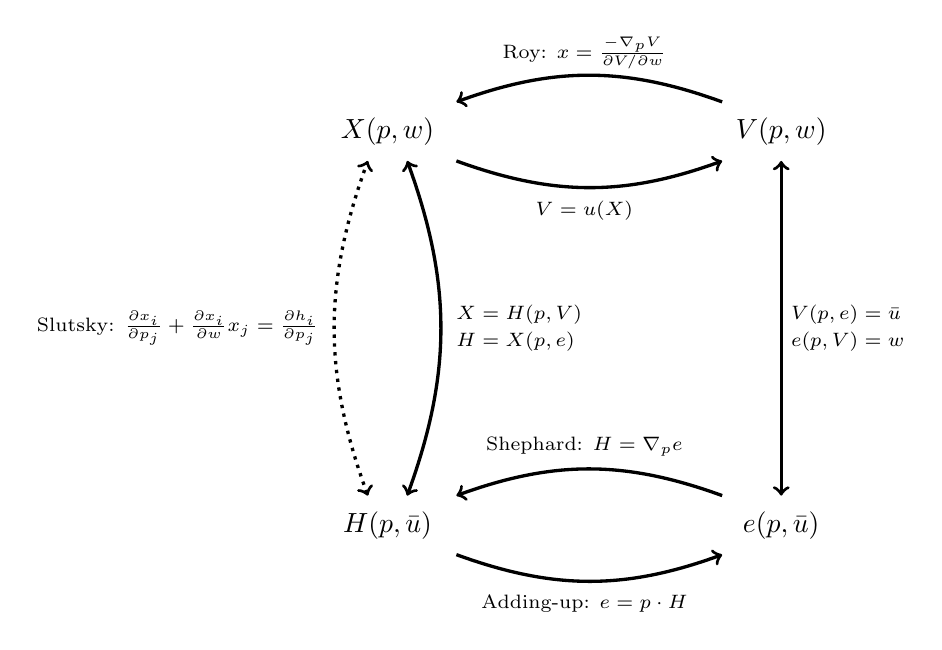
\begin{tikzpicture}[scale=0.5]
		\node at (0,10) {$X(p,w)$};
		\node at (0,0) {$H(p,\bar{u})$};
		\node at (10,0) {$e(p,\bar{u})$};
		\node at (10,10) {$V(p,w)$};
		
		\draw[<->, very thick] (0.5,0.75) to[out=70,in=-70] (0.5,9.25);
		\draw[<->, dotted, very thick] (-0.5,0.75) to[out=110,in=-110] (-0.5,9.25);
		
		\draw[<->,very thick] (10,0.75)--(10,9.25);
		
		\draw[->,very thick] (1.75,-0.75) to[out=-20,in=200](8.5,-0.75);
		\draw[<-,very thick] (1.75,0.75) to[out=20,in=-200](8.5,0.75);
		
		\draw[->,very thick] (1.75,9.25) to[out=-20,in=200](8.5,9.25);
		\draw[<-,very thick] (1.75,10.75) to[out=20,in=-200](8.5,10.75);
		
		\node at (5,2) {\scriptsize Shephard: $H = \nabla_p e$};
		\node at (5,-2) {\scriptsize Adding-up: $e = p \cdot H$};
		\node[right] at (10,5.35) {\scriptsize $V(p,e) = \bar{u}$};
		\node[right] at (10,4.65) {\scriptsize $e(p,V) = w$};
		
		\node[left] at (-1.5,5) {\scriptsize Slutsky: $\frac{\partial x_i}{\partial p_j} + \frac{\partial x_i}{\partial w} x_j = \frac{\partial h_i}{\partial p_j}$};
		\node[right] at (1.5,5.35) {\scriptsize $X = H(p,V)$};
		\node[right] at (1.5,4.65) {\scriptsize $H = X(p,e)$};
		
		\node at (5,12) {\scriptsize Roy: $x = \frac{-\nabla_p V}{\partial V / \partial w}$};
		\node at (5,8) {\scriptsize $V = u(X)$};
	\end{tikzpicture}
	\caption{Relationships Between UMP and EMP}
	\label{fig:ump_emp_relationships}
\end{figure}

\newpage
\section{Producer Theory (Harris)}\label{sec:harris}

\subsection{Classical Producer Theory}

\subsubsection{Setup}

We will always assume the following:

\begin{assumption}
	There are $L$ commodities, with a production plan $y \in \reals^L$. A net input is an element $i$ such that $y_i < 0$, and a net output is an element $j$ such that $y_j > 0$. We have a production possibilities set $Y \subseteq \reals^L$, and we assume that prices $p \ge 0$ that are unaffected by the activity of the firm.
\end{assumption}

We will also often assume, for simplicity (and in order to work with functions rather than correspondences):
\begin{assumption}
	$Y$ is nonempty, closed, and (strictly) convex, and (the \blue{free disposal property}) if $y \in Y$ and $y' \le y$, then $y' \in Y$.
\end{assumption}

\begin{definition}
	A production plan $y \in Y$ is \blue{efficient} if there does not exist $y' \in Y$ such that $y' \ge y$ and $y_i' > y_i$ for some $i$.
\end{definition}

In the case of a single output, we partition $y$ into output $q \in \reals_+$ and inputs $z \in \reals^{L-1}_+$. This allows us to define the following:

\begin{definition}
	The \blue{production function} $f:\reals^{L-1}_+ \to \reals_+$ is defined by 
	\[
	f(x) = \max q \st (q,-z) \in Y
	\]
\end{definition}

\begin{definition}
	The \blue{input requirement set}
	\[
	V(q) \coloneqq \{z \in \reals_+^{L-1} : (q,-z) \in Y\}
	\]
	gives all of the input vectors that can be used to produce an output $q$.
\end{definition}

\begin{definition}
	The \blue{isoquant} 
	\[
	Q(q) \coloneqq \{z \in \reals_+^{L-1} : z \in V(q) \text{ and } z \not\in V(q') \text{ for any } q' > q\}
	\]
	gives all the input vectors that can be used to produce at most $q$ units of output.
\end{definition}

\subsubsection{Cost Minimization}

We will make the following assumptions through this section:

\begin{assumption}
	There are $L-1$ inputs $z$, and one output $q = f(z)$. The production function $f$ is twice continuously differentiable, and inputs have price $w \in \reals^{L-1}_+$
\end{assumption}
\begin{remark}
	If any input has price zero, the firm will obviously not consider it in its decision making.
\end{remark}

\begin{definition}
	The firm's \blue{cost minimization problem} is
	\[
	\min_{z \in \reals^{L-1}_+} w \cdot z \st f(z) = q
	\]
	The associated value function is called the \blue{cost function}
	\[
	C(w,q) \coloneqq \min_{z \in \reals^{L-1}_+} w \cdot z \st f(z) = q
	\]
\end{definition}

\begin{proposition}\label{prop:cost_fn_properties}
	\red{(Properties of the Cost Function)}
	
	\begin{itemize}
		\item[(i)] $C$ is homogeneous of degree 1 in $w$
		\item[(ii)] $C$ is concave in $w$
		\item[(iii)] If we assume free disposal, $C$ is nondecreasing in $q$
		\item[(iv)] If $f$ is homogeneous of degree $k$ in $z$, $C$ is homogeneous of degree $\frac{1}{k}$ in $q$
	\end{itemize}
\end{proposition}
\begin{proof}
	
	\begin{itemize}
		\item[(i)] Increasing $w$ by $\alpha > 0$ is a monotonic transformation and does not affect the choice of $z$, but it does increase $w \cdot z$ by a factor of $\alpha$.
		\item[(ii)] Fix $w,w' \in \reals^{L-1}_+$, and suppose $C(w,q) = w \cdot z$ and $C(w',q) = w' \cdot z'$. Take $\alpha \in [0,1]$ and let $w'' = \alpha w + (1-\alpha)w'$. Then for $z''$ a cost minimizer at $w''$, we have that
		\[
		C(w'',q) = w'' \cdot z'' = \alpha w \cdot z'' + (1-\alpha)w' \cdot z''
		\]
		We also know that $w \cdot z'' \ge C(w,q)$ and $w'\cdot z'' \ge C(w',q)$, so we have that $C(w'',q) \ge \alpha C(w,q) + (1-\alpha)C(w',q)$.
		\item[(iii)] Suppose that $q' > q$. By free disposal, $q$ can be produced using the same input vector used to produce $q'$.
		\item[(iv)] Homogeneity of degree $k$ of $f$ implies that 
		\[
		f(z) = q \Longleftrightarrow \frac{1}{q} f(z) = 1 \Longleftrightarrow f\parl \frac{z}{q^{1/k}}\parr = 1
		\]
		Thus, we get that
		\begin{align*}
			C(w,q) &= \min_{z}w \cdot z \st f\parl \frac{z}{q^{1/k}}\parr = 1 \\
			&= q^{1/k} \min_z w \cdot \frac{z}{q^{1/k}} \st f\parl \frac{z}{q^{1/k}}\parr = 1  \\
			&= q^{1/k} C(w,1)
		\end{align*}
	\end{itemize}
\end{proof}

\subsubsection{Homogeneous Functions (a brief aside)}

\begin{definition}
	A function $f: X \subseteq \reals^n \to \reals$ is \blue{homogeneous of degree $k$} if
	\[
	f(\alpha x) = \alpha^k f(x) \forall \alpha > 0, x \in X
	\]
	where $k$ is a non-negative integer.
\end{definition}
\begin{proposition}
	If a function $f$ is homogeneous of degree $k$, then any of its partial derivatives are homogeneous of degree $k-1$
\end{proposition}
\begin{proof}
	Let $f_i = \frac{\partial f}{\partial x_i}$. We have that
	\[
	f(\alpha x) = \alpha^k f(x) \Longrightarrow \alpha f_i(\alpha x) = \alpha^k f_i(x) \Longrightarrow f_i(\alpha x) = \alpha^{k-1}f_i(x)
	\]
\end{proof}

\begin{proposition}
	\red{(Euler's Formula)} If $f$ is homogeneous of degree $k$ and differentiable, then at any $x$
	\[
	\sum_{i=1}^n \frac{\partial f(x)}{\partial x_i}x_i = kf(x)
	\]
\end{proposition}
\begin{proof}
	Differentiating with respect to $\alpha$ and evaluating at $\alpha = 1$, we get that
	\[
	f(\alpha x) = \alpha^k f(x) \Longrightarrow \sum_{i=1}^n f_i(\alpha x) x_i = k\alpha^{k-1}f(x) \Longrightarrow \sum_{i=1}^n f_i(x)x_i = kf(x)
	\]
\end{proof}

\begin{proposition}
	If the production function $f$ is homogeneous of degree $k$, then
	\[
	\textnormal{MRTS}_{ij}(z) \coloneqq \frac{\frac{\partial f(z)}{\partial z_i}}{\frac{\partial f(z)}{\partial z_j}} = \frac{\frac{\partial f(\alpha z)}{\partial z_i}}{\frac{\partial f(\alpha z)}{\partial z_j}} \eqqcolon \textnormal{MRTS}_{ij}(\alpha z)
	\]
\end{proposition}
\begin{proof}
	\[
	\frac{f_i(\alpha z)}{f_j(\alpha z)} = \frac{\alpha^{k-1}f_i(z)}{\alpha^{k-1}f_j( z)} = \frac{f_i(z)}{f_j(z)}
	\]
\end{proof}

\subsubsection{Profit Maximization}

\begin{definition}
	The firm's \blue{profit maximization problem} is
	\[
	\max_y p \cdot y \st y \in Y
	\]
	The associated value function is called the \blue{profit function}:
	\[
	\pi(p) \coloneqq \max_y p \cdot y \st y \in Y
	\]
\end{definition}

\begin{remark}
	In the single output case, this becomes
	\[
	\pi(p,w) \coloneqq \max_y p f(z) - w \cdot z 
	\]
	Henceforth, we consider only the single output case.
\end{remark}
\begin{remark}
	Note that profit maximization implies cost minimization.
\end{remark}

\begin{proposition}\label{prop:profit_properties}
	\red{(Properties of the Profit Function)}
	\begin{itemize}
		\item[(i)] Homogeneous of degree 1
		\item[(ii)] Nondecreasing in $p$
		\item[(iii)] Nonincreasing in $w$
		\item[(iv)] Convex in $(p,w)$
		\item[(v)] Continuous
	\end{itemize}
\end{proposition}
\begin{proof}
	\begin{itemize}
		\item[(i)] $\max_z \alpha (pf(z) - w\cdot z) = \alpha \max_z pf(z) - w\cdot z$
		\item[(ii)] $p' \ge p \Longrightarrow p' f(z) \ge p f(z) \forall z$
		\item[(iii)] $w' \ge w \Longrightarrow w' \cdot z \ge w \cdot z$
		\item[(iv)] Let $(p'',w'') := \alpha (p,w) + (1-\alpha)(p',w')$ and let $z,z',z''$ be the solution to the profit maximization problem with the corresponding output prices and input price vectors. Then by definition
		\[
		\pi(p,w) = pf(z) - w \cdot z \ge p f(z'') - w \cdot z''
		\]
		\[
		\pi(p',w') = p'f(z) - w' \cdot z \ge p' f(z'') - w' \cdot z''
		\]
		which implies that
		\begin{align*}
		\alpha \pi(p,w) + (1-\alpha)\pi(p',w') &\ge \alpha (p f(z'') - w \cdot z'') + (1-\alpha) ( p' f(z'') - w' \cdot z'') \\
		&= (\alpha p + (1-\alpha)p') f(z'') - (\alpha w + (1-\alpha)w' )\cdot z'' \\
		&= \pi(p'',w'')
		\end{align*}
		\item[(v)] Follows from Berge's Theorem
	\end{itemize}
\end{proof}

\begin{remark}
	$\pi$ being convex in $(p,w)$ implies that $\pi$ is convex in $p$ and $w$ individually.
\end{remark}

\begin{definition}
	The \blue{unconditional input demand function}
	\[
	x(p,w) \coloneqq \argmax_{z \in \reals^{L-1}_+} pf(z) - w\cdot z
	\]
	is the solution to the profit maximization problem. The \blue{output supply function}
	\[
	q(p,w) \coloneqq f(x(p,w))
	\]
	is the output level where the profit is being maximized.
\end{definition}

\begin{proposition}\label{prop:hotelling}
	\red{(Hotelling's Lemma)} If $\pi$ is differentiable, then for $(p,w) \in \reals^L_{++}$,
	\begin{align*}
		q(p,w) &= \frac{\partial \pi(p,w)}{\partial p} \\
		x_j(p,w) &= -\frac{\partial \pi(p,w)}{\partial w_j}
	\end{align*}
\end{proposition}
\begin{proof}
	(Sketch) Apply the Envelope Theorem, and note that $x(p,w)$ is the profit maximizing bundle and $q(p,w)$ is the production function evaluated at that bundle.
\end{proof}

\begin{remark}
	This condition can be relaxed from differentiability to the unconditional input demand function and output supply function being well-defined functions.
\end{remark}

\begin{definition}
	The \blue{conditional input demand function} 
	\[
	z(w,q) \coloneqq \argmin_{z \in \reals^{L-1}_+} w \cdot z \st f(z) = q
	\]
	is the solution to the cost minimization problem.
\end{definition}

\begin{proposition}
	\red{(Shephard's Lemma)} If $C$ is differentiable, then for $w \in \reals^{L-1}_{++}$,
	\[
	z_i(w,q) = \frac{\partial C(w,q)}{\partial w_i}
	\]
\end{proposition}
\begin{proof}
	(Sketch) Similarly, apply the Envelope Theorem to the cost minimization problem.
\end{proof}

\begin{proposition}
	Suppose the profit function is twice continuously differentiable. Then:
	\begin{itemize}
		\item[(i)] $\frac{\partial q(p,w)}{\partial p_i} \ge 0$
		
		\item[(ii)] $\frac{\partial x_j(p,w)}{\partial w_j} \le 0$
		
		\item[(iii)] $\frac{\partial x_j(p,w)}{\partial w_i} = \frac{\partial x_i(p,w)}{\partial w_j}$
	\end{itemize}
\end{proposition}
\begin{proof}
	Note that the profit function being twice continuously differentiable and convex implies that its Hessian is positive semdefinite. Conclusion follows from applying Hotelling's Lemma
\end{proof}

\begin{proposition}
	Suppose the cost function is twice continuously differentiable. Then:
	\begin{itemize}
		\item[(i)] $\frac{\partial z_i(w,q)}{\partial w_i} \le 0$
		
		\item[(ii)] $\frac{\partial z_j(w,q)}{\partial w_i} = \frac{\partial z_i(w,q)}{\partial w_j}$
		
		\item[(iii)] $\frac{\partial z_i(w,q)}{\partial q} = \frac{\partial MC(w,q)}{\partial w_i} = \begin{cases} > 0 & \textnormal{Normal Input} \\ < 0 & \textnormal{Inferior Input} \end{cases}$
	\end{itemize}
\end{proposition}
\begin{proof}
	(i) follows from $C$ being concave in $w$. (ii) and (iii) follow from the symmetry of second derivatives of $C$.
\end{proof}

\subsubsection{Comparative Statics}

\begin{remark}
	For a full treatment, including a few producer theory examples, see Tak's notes on Comparative Statics.
\end{remark}

\begin{assumption}
	Two inputs $(x_1,x_2)$, one output $q = f(x)$. $f \in C^2$ and the Hessian $H_f$ is negative definite. $f(0,x_2) = f(x_1,0) = 0$, so both inputs are necessary. Inada conditions on $x_1,x_2$, output price $p > 0$, input prices $w \gg 0$.
\end{assumption}

Consider the profit maximization problem
\[
\max_{x \in \reals^2_{++}} pf(x) - wx
\]

\begin{exercise}
	Prove that $\partial x_1(p,w) / \partial w_1 < 0$. Taking FOC, we get
	\[
	pf_1(x) - w_1 = 0 \quad \text{ and }\quad pf_2(x) - w_2 = 0
	\]
	We have that the Hessian of $x$, $H_x$, is 
	\[
	H_x = p \matrixc{f_{11} & f_{12} \\ f_{21} & f_{22}} = pH_f
	\]
	Since $H_f$ is negative definite, this matrix is invertible. By the Implicit Function Theorem, FOCs implicitly define $x(p,w) = (x_1(p,w), x_2(p,w))$, and we can rewrite them as
	\[
	pf_1(x(p,w)) - w_1 = 0 \quad \text{ and } \quad pf_2(x(p,w)) - w_2 = 0
	\]
	Taking derivatives with respect to $w_1$, we get
	\[
	pf_{11} \frac{\partial x_1}{\partial w_1} + p f_{12} \frac{\partial x_2}{\partial w_1} = 1
	\]
	\[
	pf_{21} \frac{\partial x_1}{\partial w_1} + p f_{22} \frac{\partial x_2}{\partial w_1} = 0
	\]
	which gives us
	\[
	p \matrixc{f_{11} & f_{12} \\ f_{21} & f_{22}} \matrixc{\partial x_1 / \partial w_1 \\ \partial x_2 / \partial w_1} = \matrixc{1 \\ 0}
	\]
	We get that
	\begin{align*}
	\matrixc{\partial x_1 / \partial w_1 \\ \partial x_2 / \partial w_1} &= \frac{1}{p} \frac{1}{f_{11}f_{22} - f_{12} f_{21}} \matrixc{f_{22} & -f_{12} \\ -f_{21} & f_{11}} \matrixc{1 \\ 0} \\
	&= \frac{1}{p} \frac{1}{f_{11}f_{22} - f_{12} f_{21}} \matrixc{f_{22} \\ -f_{21}}
	\end{align*}
	Note that $f_{11}f_{22} - f_{12}f_{21} > 0$, because $H_f$ is negative definite, and that $f_{22} < 0$, which means that $\frac{\partial x_1}{\partial w_1} < 0$.
\end{exercise}

\begin{question}
	Why is it worth studying cost minimization and profit maximization separately? There are some settings where profit maximization might be unreasonable:
	\begin{itemize}
		\item Dynamics. For example, if there is learning by doing, this gives a firm incentives to choose $q > q(p,w)$ today in order to decrease tomorrow's costs
		\item Managerial utility maximization. If a larger firm gives more prestige, might have $q > q(p,w)$
	\end{itemize}
\end{question}



\subsection{Non-Price-Taking Firms}

In our assumptions, we said that firms were unaffected by the firm's activity. This leads to the simple problem we've been working in:
\[
\max_{z \in \reals^{L-1}} pf(z) - wz
\]
If their output has market power, then we have
\[
\max_{z \in \reals^{L-1}} p(f(z))f(z) - wz
\]
And we assume that $p'(q) < 0 \forall q$. They could also have input market power:
\[
\max_{z \in \reals^{L-1}} pf(z) - w(z)z
\]
where we assume that $\frac{\partial w_i(z)}{\partial z_i} > 0$ and $\frac{\partial w_i(z)}{\partial z_j} = 0 \forall i \ne j$. 


These problems imply that:
\begin{center}
	\begin{tabular}{| c | c | c | c | }
		\hline
		 Statistic & No MP & Output MP & Input MP \\
		 \hline
		 FOCs & $p \nabla f(z) = w$ & $[p(f(z)) + p'(f(z))f(z)] \nabla f(z) = w$ & $p f_i(z) = w_i'(z_i)z_i + w_i(z_i)$\\
		 \hline
		 MRTS & $\frac{f_i(z)}{f_{i'}(z)} = \frac{w_i}{w_{i'}}$ & $\frac{f_i(z)}{f_{i'}(z)} = \frac{w_i}{w_{i'}}$ & $\frac{f_i(z)}{f_{i'}(z)} = \frac{w_i'(z_i)z_i + w_i(z_i)}{w_{i'}'(z_{i'})z_{i'} + w_{i'}(z_{i'})}$\\
		 \hline
	\end{tabular}
\end{center}

We have that profit maximization implies cost minimization in each world, with slight differences. We have that with no market power,
\begin{align*}
	\pi(p,w) &\equiv \max_{z \in \reals^{L-1}} pf(z) - w \cdot z \\
	&= \max_q \barl \max_{z \in \reals^{L-1}} pq - w \cdot z \st f(z) = q \barr \\
	&= \max_q p\cdot q - \barl \min_{z \in \reals^{L-1}} w \cdot z \st f(z) = q \barr \\
	&=  \max_q p\cdot q - C(w,q)
\end{align*}
With output market power, this becomes
\begin{align*}
	\pi(p,w) &\equiv \max_{z \in \reals^{L-1}} p(f(z))f(z) - w \cdot z \\
	&= \max_q \barl \max_{z \in \reals^{L-1}} p(q)q - w \cdot z \st f(z) = q \barr \\
	&= \max_q p(q)\cdot q - \barl \min_{z \in \reals^{L-1}} w \cdot z \st f(z) = q \barr \\
	&=  \max_q p(q)\cdot q - C(w,q)
\end{align*}
With input market power, we have
\begin{align*}
	\pi(p,w) &\equiv \max_{z \in \reals^{L-1}} pf(z) - w(z) \cdot z \\
	&= \max_q \barl \max_{z \in \reals^{L-1}} pq - w(z) \cdot z \st f(z) = q \barr \\
	&= \max_q p\cdot q - \barl \min_{z \in \reals^{L-1}} w(z) \cdot z \st f(z) = q \barr \\
	&=  \max_q p\cdot q - C(q)
\end{align*}

Under perfect competition, there is no profit -- the FOCs imply that
\[
p = \frac{\partial }{\partial q} C(w,q) \text{ \ie, price is marginal cost}
\]
With output market power, we have that
\[
p(q^m) + p'(q^m)q^m = \frac{\partial }{\partial q} C(w,q^m)
\]
which implies that
\[
p(q^m) = \frac{\partial }{\partial q} C(w,q^m) - \underbrace{p'(q^m)}_{<0}q^m > \frac{\partial}{\partial q} C(w,q^m)
\]
so there is positive profit. This with quantity choice. We can equivalently look at the price choice problem. We have
\[
\max_p p D(p) - c(w,D(p)) \Longrightarrow [p^m D'(p^m) + D(p^m)] = \frac{\partial}{\partial q} C(w,D(p^m)) D'(p^m)
\]
which implies that
\begin{align*}
	p^m - \frac{\partial}{\partial q}C(w,q^m) &= -\frac{D(p^m)}{D'(p^m)} \\
	p^m &= \parl \frac{\varepsilon}{1 + \varepsilon}\parr \frac{\partial}{\partial q} C(w,D(p^m))
\end{align*}
where $\varepsilon$ is the negative inverse of the Lerner index.

With input market power (supposing for simplicity that there is only one input), we have
\[
\max_z pf(z) - w(z)z
\]
Since $w(z)$ is increasing, we can write its inverse $z(w)$, and get
\[
\max_w pf(z(w)) - w z(w)
\]
and the FOC get us
\begin{align*}
	p f'(z(w)) z'(w) &= z'(w) w  + z(w) \\
	p \frac{f'(z(w))}{w} &= \frac{z(w)}{z'(w)w} + 1 \\
	p \frac{f'(z(w))}{w} &= \frac{1}{\varepsilon_{z,w}} + 1 = \frac{1 + \varepsilon_{z,w}}{\varepsilon_{z,w}} \\
	w &= \parl \frac{\varepsilon_{z,w}}{1 + \varepsilon_{z,w}} \parr p f'(z(w)) < p f'(z(w))
\end{align*}
where $\varepsilon_{z,w}$ is the elasticity of input supply.

\newpage
\section{Uncertainty Theory (Blume)}\label{sec:blume}

\textbf{\emph{n.b.}} Prof. Blume did not prove any of the results presented here. It clearly matters more that one understands the intuition rather than the exact proof structure. Proof sketches are added wherever possible. I have relied on \href{https://www.semanticscholar.org/paper/Utility-theory-for-decision-making-Fishburn/905a24a912171436e0abd3b5f1fdcb963e6f852f}{Fishburn (1970)} for these proof sketches.

\subsection{Models of Preferences}\label{subsec:models_blume}

\begin{remark}
	There are three main preference models that we will consider here: \href{https://psycnet.apa.org/record/1947-03159-000}{von Neumann and Morgenstern (1947)}, where the objects of choice are probability distributions on outcomes; \href{https://psycnet.apa.org/record/1955-00117-000}{Savage (1954)}, where the objects of choice are outcome-valued random variables (formally, functions from states of the world to outcomes); and \href{https://pages.stern.nyu.edu/~dbackus/Exotic/1Ambiguity/AnscombeAumann\%20AMS\%2063.pdf}{Anscombe and Aumann (1963)}, where the objects of choice are functions from states of the world to probability distributions over outcomes.
\end{remark}

\begin{model}
	\red{von Neumann--Morgenstern} We have $X$ a set of \blue{outcomes} (or prizes) and $P$ the set of probability distributions on $X$, called \blue{lotteries}. For each $p \in P$, we define the \blue{support} of $p$ as
	\[
	\text{supp } p = \{x \in X : p(x) > 0\}
	\]
	A preference relation $\succsim$ on $P$ has an \blue{expected utility representation} if there is a real-valued function $u: X \to \reals$ such that
	\[
	p \succsim q \Longleftrightarrow \sum_{x \in \text{supp } p} u(x)p(x) \ge \sum_{y \in \text{supp } q} u(y)q(y)
	\]
\end{model}

\begin{remark}
	In general, people are inconsistent on what they call $u$. Here, we refer to it as the \blue{Bernoulli Utility Function}, following MWG. Prof. Blume also referred to it as the \blue{payoff function}.
\end{remark}

\begin{remark}
	In this model, whenever $X$ is finite, indifference curves are linear in probabilities. See Figure~\ref{fig:indifference_probability}, where indifference curves are in red.
	
	\begin{figure}[H]
		\centering
		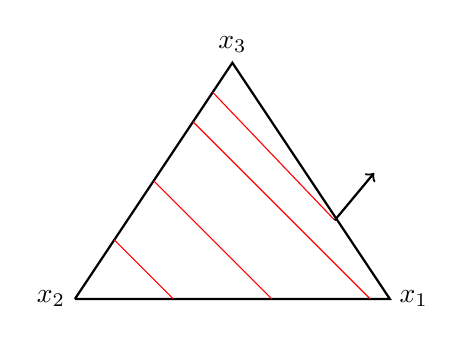
\begin{tikzpicture}[scale=1]
			\draw[thick] (0,0)--(2,3)--(4,0)--(0,0);
			\node[above] at (2,3) {$x_3$};
			\node[right] at (4,0) {$x_1$};
			\node[left] at (0,0) {$x_2$};
			
			\draw[red] (1,1.5)--(2.5,0);
			\draw[red] (0.5,0.75)--(1.25,0);
			\draw[red] (1.5,2.25)--(3.75,0);
			\draw[red] (1.75,2.625)--(3.3,1);
			
			\draw[->,thick] (3.3,1)--(3.8,1.6);
		\end{tikzpicture}
		\caption{Indifference Curves Over Probability Distributions}
		\label{fig:indifference_probability}
	\end{figure}
\end{remark}


\begin{model}
	\red{Savage} We have $X$ a set of outcomes, $S$ a set of \blue{states of the world}, and $F$ the set of \blue{Savage acts}, where $f \in F$ is a function $f : S \to X$. A preference relation $\succsim$ on $F$ has an expected utility representation if there is a probability distribution $p$ on $S$ and a real-valued function $u: X \to \reals$ such that
	\[
	f \succsim g \Longleftrightarrow \sum_{s \in S} u(f(s))p(s) \ge \sum_{s \in S} u(g(s))p(s)
	\]
\end{model}

\begin{model}
	\red{Anscombe--Aumann} We have $X$ a set of outcomes, $S$ a set of states of the world, $P$ the set of probability distributions on $X$, and $A$ the set of \blue{Anscombe--Aumann Acts}, where $a \in A$ is a function $a: S \to P$. A preference relation $\succsim$ on $A$ has an expected utility representation if there is a probability distribution $p$ on $S$ and a real-valued function $u: X \to \reals$ such that
	\[
	a \succsim b \Longleftrightarrow \sum_{s \in S} \sum_{x \in X} u(x) \parl a(s) (x)\parr p(s) \ge \sum_{s \in S} \sum_{x \in X} u(x) \parl b(s) (x)\parr p(s)
	\]
\end{model}

\subsection{von Neumann--Morgenstern}

We first introduce a famous paradox:

\begin{example}
	\red{The St. Petersburg Paradox} A fair coin is tossed until tails appears. How much would you pay for a lottery ticket that paid off $2^n$ dollars if the first tails appears on the $n$th flip? The expected value of this lottery is
	\[
	EV = \frac{1}{2} \cdot 2 + \frac{1}{4}\cdot 4 + \cdots = 1 + 1 + \cdots = \infty
	\]
	However, clearly it's not reasonable to pay a massive amount of money for this lottery ticket. Why is this happening? There are a few explanations, and we'll go through them in this section.
\end{example}

We make the following assumptions on preferences:

\begin{assumption}\label{ass:vnm}
(referred to as the `Finite $X$ Axioms' by Prof. Blume)
	\begin{itemize}
		\item[(i)] $\succsim$ is complete and transitive
		\item[(ii)] (Independence) For all $0 < \alpha \le 1$ and all $r \in P$,
		\[
		p \succsim q \Longleftrightarrow \alpha p + (1-\alpha)r \succsim \alpha 1 + (1-\alpha)r
		\]
		\item[(iii)] (Archimedean) If $p \succ q \succ r$, then there exists $\alpha,\beta \in (0,1)$ such that
		\[
		\alpha p + (1-\alpha) r \succ q \succ \beta p + (1-\beta)r
		\]
	\end{itemize}
\end{assumption}

\begin{theorem}\label{thm:vnm}
	\red{(von-Neumann--Morgenstern Theorem)} If $\succsim$ satisfies Assumptions~\ref{ass:vnm}, then $\succsim$ has an expected utility representation; there is a function $u: X \to \reals$ such that
	\[
	p \succsim q \Longleftrightarrow \sum_{x \in X} u(x)p(x) \ge \sum_{x \in X} u(x)q(x)
	\]
	Furthermore, if $v: X \to \reals$ is another expected utility representation, then there are constants $\alpha > 0$ and $\beta$ such that $v(x) \equiv \alpha u(x) + \beta$.
\end{theorem}
\begin{proof}
	(Very rough sketch) We will define the distance between two lotteries $p$ and $q$ as a function over a subset of a convex cone in an arbitrary metric space, which exists due to the fact that $X$ is finite. This is mathematically tricky, but actually much easier in low-dimensional Euclidean space. You can imagine what's happening by considering the positive-positive quadrant of $\reals^2$, which is a convex cone. From there, the assumptions give us that the cone is convex and compact, and the relationship we are looking for follows directly from the Extreme Value Theorem, considering the roots of the distance function. The second conclusion follows directly from the fact that affine transformations preserve convexity and extrema.
\end{proof}

\begin{definition}
	A \blue{simple lottery} is $p:= (p_1 : x_1,p_2:x_2,\dots,p_K:x_K)$, where $x_1,\dots,x_K$ are outcomes in $\reals$ and $p_1,\dots,p_K$ are probabilities. Let $\mathcal{L}$ denote the set of simple lotteries, and let $u: X \to \reals$ and $U(p) = \sum_{k} u(x_k)p_k$. Formally, this is the expectation of the random variable $u(x)$, itself a function of the random variable $x$, where $x \sim p$.
\end{definition}

\begin{question}
	How do we see that this is linear in lotteries? How do we mix lotteries?
\end{question}

For lotteries with common support, mixing is just the convex combination of the probabilities. But what happens when lotteries have different supports?

\begin{example}
	Consider $p \coloneqq (p_1:x_1,p_2:x_2)$ and $q\coloneqq (q_1:y_1,q_2:y_2,q_3:y_3)$. We can say that
	\[
	p\oplus_\alpha q = (\alpha p_1:x_1, \alpha p_2: x_2,(1-\alpha)q_1:y_1, (1-\alpha)q_2:y_2, (1-\alpha)q_3:y_3)
	\]
	\begin{remark}
		This is \emph{not} a convex combination! It combines objects of different sizes. However, expected utility is still linear:
		\begin{align*}
			U(p \oplus_\alpha q) &= \sum_{k=1}^2 \alpha p_k u(x_k) + \sum_{k=1}^3 (1-\alpha)q_ku(y_k) \\
			&= \alpha \sum_{k=1}^2 p_k u(x_k) +(1-\alpha) \sum_{k=1}^3 q_ku(y_k) \\
			&= \alpha U(p) + (1-\alpha)U(q)
		\end{align*}
	\end{remark}
\end{example}

\begin{definition}
	(From \href{https://www.jstor.org/stable/1905540}{Herstein and Milnor (1953)}) A \blue{mixture space} is a set of objects $\Pi$, with typical elements $\pi,\rho,\mu,\nu$ and a family of functions for $0 \le \alpha \le 1$, $\oplus_\alpha : \Pi \times \Pi \to \Pi$ such that
	\begin{itemize}
		\item[(i)] $\pi \oplus_1 \rho = \pi$
		\item[(ii)] $\pi \oplus_\alpha \rho = \rho \oplus_{1-\alpha} \pi$
		\item[(iii)] $(\pi \oplus_\beta \rho) \oplus_\alpha \rho = \pi \oplus_{\alpha\beta} \rho$
	\end{itemize}
	where $\beta \in [0,1]$.
\end{definition}

Some examples:
\begin{itemize}
	\item Convex sets with the operation of convex combinations
	\item Simple probability distributions on convex sets
	\item $S$ and $X$ are sets, and let $M$ denote the set of functions from $S$ to probability distributions on $X$. The $\oplus_\alpha$ are the (pointwise) convex combinations of these functions
\end{itemize}

We can update Assumptions~\ref{ass:vnm} with the mixture space definitions:
\begin{assumption}\label{ass:vnm_mix}
	(i) remains the same. The others:
	
	\begin{itemize}
		\item[(ii)] (Independence) For all $0 < \alpha \le 1$ and all $r \in P$, $p \succsim q \Longrightarrow p \oplus_\alpha r \succsim q \oplus_\alpha r$
		
		\item[(iii)] (Archimedean) If $p \succ q \succ r$, then there exist $\alpha,\beta \in (0,1)$ such that $p \oplus_\alpha r \succ q \succ p \oplus_\beta r$
	\end{itemize}
\end{assumption}

We can also update Theorem~\ref{thm:vnm} to generalize it:
\begin{theorem}\label{thm:vnm_mix}
	If $M$ is a mixture space and $\succsim$ satisfies Assumptions~\ref{ass:vnm_mix}, then there exists a linear function $U: M \to \reals$. Any other linear representation $V$ is a positive affine transformation of $U$.
\end{theorem}

\paragraph{Some Criticisms.} First, the Archimedean property seems quite odd. What happens if one outcome is infinitely preferred to another?

\begin{example}
	Suppose that we have outcomes $x,y,z$ occurring with probabilities $\rho_x,\rho_y,\rho_z$. Further assume that $x$ is \emph{infinitely better} than $y$ and $z$. We have the following (lexicographic, so rational) preference relation: $(\rho_x,\rho_y,\rho_z) \succ(\rho_x',\rho_y',\rho_z')$ if $\rho_x > \rho_x'$ or if $\rho_x = \rho_x'$ and $\rho_y > \rho_y'$. These preferences lead to a counterexample. Let $p = (1,0,0)$, $r = (0,3/4,1/4)$, and $r = (0,1/4,3/4)$. Then $p \succ q \succ r$. For all $\alpha \in (0,1)$, however,
	\[
	\alpha p + (1-\alpha)r = (\alpha, (1-\alpha)/4,3(1-\alpha)/4) \succ q
	\]
\end{example}
To fix this, we will often assume that $X$ has no infinitely large or small elements.

Another criticism is independence. Are preferences linear in probabilities? The following is another famous paradox:

\begin{example}
	\red{The Allais Paradox} (from \href{https://www.jstor.org/stable/1907921}{Allais (1953)}). Consider the following lotteries:
	\[
	A = \begin{cases}\$1\text{M} & p = 1\end{cases}\qquad B = \begin{cases} \$1\text{M} & p = 0.89 \\ \$5\text{M} & p = 0.10 \\ \$0 & p = 0.01\end{cases}
	\]
	\[
	C = \begin{cases}\$1\text{M} & p = 0.11 \\ \$0 & p = 0.89\end{cases}\qquad D = \begin{cases} \$5\text{M} & p = 0.10 \\  \$0 & p = 0.90\end{cases}
	\]
	Most people prefer $A$ to $B$, and prefer $D$ to $C$. This violates the independence axiom.
\end{example}

This paradox can be resolved by strengthening the Archimedean assumption. This requires some topological considerations beyond this course, but admits an expected utility representation such that $u$ is now bounded and continuous.


\begin{remark}
	Thinking back to the St. Petersburg Paradox, we can now look at some solutions posed.
	\begin{enumerate}
		\item Bernoulli suggested that people tend to disregard small probabilities, rounding them to zero. This became, much later, the foundation of Prospect Theory.
		\item Cramer suggested expected utility, the first time it was used! With some assumptions (mainly, that $u$ must be bounded), this resolves the paradox
	\end{enumerate}
\end{remark}

\subsection{Subjective Probability}

We tend to think of three regimes for where probability comes from:
\begin{enumerate}
	\item \blue{Frequentist}: Probabilities exist, and can in principle be measured by repeated experiments.
	\item \blue{Logical}: Probabilities are the weight that an event happens based on evidence. It essentially generalizes truth from $\{0,1\}$ to $[0,1]$
	\item \blue{Bayesian}: Probability is the degree of belief people have that an event will occur
\end{enumerate}

Before thinking deeply about subjective expected utility theory, we need some mathematical background. Here are presented some definitions and results, without proof.

\begin{definition}
	Suppose that $S$ is finite. Suppose that $\mathcal{S}$ is a collection of subsets of $S$ such that (i) $\emptyset \in \mathcal{S}$, (ii) if $A \in \mathcal{S}$, then $A^c \in \mathcal{S}$, and (iii) if $A,B \in \mathcal{S}$, then $A \cap B \in \mathcal{S}$. $\mathcal{S}$ is a \blue{(Boolean) algebra} of \blue{events}. When $S$ is finite, we can take $\mathcal{S} = 2^S$. When $S = \reals$, we need to take more care.
\end{definition}

\begin{definition}
	A \blue{probability} on $\mathcal{S}$ is a function $p : \mathcal{S} \to [0,1]$ such that (i) $p(\mathcal{S}) = 1$ and (ii) if $A \cap B = \emptyset$, then $p(A \cup B) = p(A) + p(B)$.
\end{definition}
\begin{definition}
	A \blue{qualitative probability} is a binary relation $\sqsubseteq$ on $\mathcal{S}$ such that
	\begin{itemize}
		\item[(i)] $\sqsubseteq$ is complete and transitive
		\item[(ii)] $\mathcal{S} \sqsupset \emptyset$
		\item[(iii)] for all $A \in \mathcal{S}$, $\emptyset \sqsubseteq A \sqsubseteq \mathcal{S}$
		\item[(iv)] If $A,B,C \in \mathcal{S}$ and $A \cap C = B \cap C = \emptyset$, then $A \sqsubseteq B \Longleftrightarrow A \cap C \sqsubseteq B \cap C$
	\end{itemize}
\end{definition}

\begin{definition}
	Let $\mathcal{A} = \{A_1,\dots,A_k\}$ and $\mathcal{B} = \{B_1,\dots,B_k\}$ be lists of events, allowing repetitions. The lists $\mathcal{A}$ and $\mathcal{B}$ are \blue{balanced} if for each state $s \in S$, the number of events containing $s$ in $\mathcal{A}$ equals that in $\mathcal{B}$.
\end{definition}

\begin{assumption}\label{ass:mathprob}
	We have the following:
	
	\begin{itemize}
		\item[(i)] $\succsim$ on $\mathcal{S}$ is complete
		\item[(ii)] (Positivity) for all $A \in \mathcal{S}$, $A \succsim \emptyset$
		\item[(iii)] (Non-triviality) $S \succ \emptyset$
		\item[(iv)] (Finite Cancellation) For all pairs of balanced lists $\mathcal{A}$ and $\mathcal{B}$, if for all $1 \le j \le k-1$, $A_j \succsim B_j$, then $B_k \succsim A_k$.
	\end{itemize}
\end{assumption}
\begin{remark}
	Finite Cencellation implies transitivity. 
\end{remark}

\begin{theorem}
	$\succsim$ satisfies Assumptions~\ref{ass:mathprob} if and only if there is a probability $\rho$ on $\mathcal{S}$ such that $A \succsim B \Longleftrightarrow \rho(A) \ge \rho(B)$ 
\end{theorem}


\subsection{The Savage Framework}

Recall that we are now in the Savage framework, defined in Section~\ref{subsec:models_blume}. First, some definitions:

\begin{definition}
	For an act $h$, define $f \mid_A h$ as getting $f(s)$ for $s \in A$, otherwise getting $h(s)$. Let $xAy$ denote the bet that pays off $x$ on $A$ and $y$ otherwise.
\end{definition}

\begin{definition}
	We say that $f \succsim g$ given $A$, denoted $f \succsim_A g$, if $f'$ and $g'$ are actions such that $f'$ agrees with $f$ on $B$, $g'$ agrees with $g$ on $B$, and $f'$ and $g'$ agree with each other outside of $A$.
\end{definition}

\begin{definition}
	An event $A$ is \blue{null} if for all $f$ and $g$, $f \succsim_A g$.
\end{definition}

\begin{definition}
	Sets are ordered $A \succsim B$ if there are outcomes $x \succ y$ such that $xAy \succsim xBy$.
\end{definition}

Now, we get the Savage Axioms:

\begin{assumption}\label{ass:savage}
	These are:
	
	\begin{itemize}
		\item[(i)] $\succsim$ is complete and transitive
		\item[(ii)] if $f \mid_A h \succ g \mid_A h$, then for all $k$, $f \mid_A k \succ g \mid_Ak$
		\item[(iii)] For outcomes $x,y$ and non-null $A$, $x \succsim_A y$ if and only if $x \succsim y$
		\item[(iv)] For outcomes $x \succ y$ and $x' \succ y'$, and sets $A,B$, $xAy \succsim xBy$ if and only if $x' A y' \succsim x' B y'$
		\item[(v)] There exist outcomes $x \succ y$
		\item[(vi)] If $f \succ g$, then for any consequence $x$ there is a partition of $S$ such that on each $S_i$, $f \mid_{S_i} h \succ g$ and $f \succ g \mid_{S_i} h$
		\item[(vii)] If $f$ and $g$ are acts and $A$ is an event such that $f(s) \succsim_A g$ for every $s \in A$, then $f\succsim_A g$; and if $f \succsim_A g(s)$ for every $s \in A$, then $f \succsim_B g$
	\end{itemize}
\end{assumption}

\begin{theorem}
	The Savage Axioms (Assumptions~\ref{ass:savage}) imply Bayes' Rule
\end{theorem}
\begin{proof}
	From the assumptions, $f \succ_A g$ if and only if for any act $h$, $f \mid_A h \succ g\mid_A h$. We have that
	\begin{align*}
		\expect_\mu \barl u(f\mid_A h)\barr &> \expect_\mu\barl u(g \mid_A h)\barr &&\Longleftrightarrow \\
		\int_S u(f \mid_A h(s)) d\mu &> \int_S u(f \mid_A g(s)) d\mu &&\Longleftrightarrow \\
		\int_A u(f(s))d\mu + \int_{A^c} u(h(s))d\mu &> \int_A u(g(s))d\mu + \int_{A^c} u(h(s))d\mu &&\Longleftrightarrow \\
		\int_A u(f(s))d\mu &> \int_A u(g(s))d\mu &&\Longleftrightarrow \\
		\int_A u(f(s))d\mu/\mu(A) &> \int_A u(g(s))d\mu/\mu(A) \\
		\expect_\mu\barl u(f) \mid A\barr &> \expect_\mu\barl u(g) \mid A\barr
	\end{align*}
\end{proof}

\subsection{Anscombe--Aumann}

\begin{remark}
	Recall that we are now in the Anscombe--Aumann framework detailed in Section~\ref{subsec:models_blume}, meaning that an expected utility representation is a function $u: X \to \reals$ and a probability distribution $\mu$ on $S$ such that
	\[
	f \succsim g \Longleftrightarrow \sum_S \sum_X u(x) f(s)(x) \mu(s) \ge \sum_S \sum_X u(x) g(s)(x) \mu(s) 
	\]
\end{remark}

To go towards an expected utility representation theorem, we need some further assumptions, beyond Assumptions~\ref{ass:vnm}.

\begin{assumption}\label{ass:aa}
	In addition to Assumptions~\ref{ass:vnm}, we assume that
	
	\begin{itemize}
		\item[(iv)] (non-triviality) For some $f,g \in A$, $f \succ g$
		\item[(v)] (state independence) If for some $s \in S$, $a \in A$, and $p,q \in P$, $h\mid_{\{s\}^c}p \succ p \succ h\mid_{\{s\}^c}q$, then for all non-null states $t$, $h \mid_{\{s\}^c} p \succ h \mid_{\{s\}^c} q$
	\end{itemize}
\end{assumption}

\begin{theorem}
	If $\succsim$ satisfies Assumptions~\ref{ass:vnm} and Assumptions~\ref{ass:aa}, then there exists a function $u: X \to \reals$ and a probability distribution $\rho$ on $S$ such that
	\[
	f \succsim g \Longleftrightarrow \sum_S \sum_X u(x) f(s)(x) \rho(s) \ge \sum_S \sum_X u(x) g(s)(x) \rho(s)
	\]
\end{theorem}
\begin{proof}
	Complicated, and ommitted. Is in \href{https://www.semanticscholar.org/paper/Utility-theory-for-decision-making-Fishburn/905a24a912171436e0abd3b5f1fdcb963e6f852f}{Fishburn (1970)}.
\end{proof}

\subsection{Beyond Expected Utility}

\begin{remark}
	There are some big issues with expected utility theory in general. Here, some of them are summarized and some possible solutions are presented.
\end{remark}

Consider first a final famous paradox:

\begin{example}
	\red{The Ellsberg Paradox} (from \href{https://www.jstor.org/stable/1884324}{Ellsberg (1961)}) There is a single urn with three balls. One ball is red and the other two are either blue or green. One ball is drawn from the urn, and the bettor bets on its color. Winning bets pay \$100, losing bets pay nothing. Available bets are red, blue, not red, and not blue. 
	
	Typical laboratory preferences are inconsistent with probabilistic beliefs -- both red and not red are preferred to blue and not blue. This is a major issue, with several proposed solutions over the years.
\end{example}

\begin{example}
	Weighted EU. One idea is that individuals overweight small-probability events. Imagine a weighting function $w: [0,1] \to [0,1]$ with $w(p) > p$ for small $p$ and $w(p) < p$ for large $p$. One issue: weighted expected utility will not respect FOSD. 
\end{example}

\begin{example}
	Rank-Dependent Expected Utility. Instead of weighing probabilities, apply probability weights to the CDF:
	\[
	U(p) = \sum_n w_n(p)u(x_n)
	\]
	where $x_1 \le x_2 \le \cdots \le x_n$ and 
	\[
	w_n(p) = q\parl \sum_{k=1}^n p_k\parr - q\parl \sum_{k=1}^{n-1}p_k\parr
	\]
	where $q: [0,1] \to [0,1]$ transforms probabilities and $q(0) = 0 = 1-q(1)$. If $q$ is strictly increasing, than $\succsim$ respects FOSD.
\end{example}

\begin{example}
	Maxmin EU. Ambiguity is the idea that individuals may be uncertain about what probability distribution they face. If, for example, you bet as if the worse case scenario were always the probability distribution for the current bet, the Ellsberg paradox would result.
\end{example}

\begin{definition}
	\blue{Choquet Expected Utility} is expected utility where the expectation is taken with respect to a non-additive probability, also called a \blue{capacity}. Suppose $S$ is finite and $\mathcal{S} = 2^S$. A function $\mu: S \to [0,1]$ is a capacity if (i) $\mu(\emptyset) = 0$, $\mu(S) = 1$, and for all $A \subset B \in S$, $\mu(B) \ge \mu(A)$. 
\end{definition}

\begin{assumption}\label{ass:choquet}
	We have the following assumptions for Choquet Expected Utility over Anscombe--Aumann acts:
	\begin{itemize}
		\item[(i)] $\succsim$ is complete and transitive
		\item[(ii)] An Archimedean axiom
		\item[(iii)] The independence axioms for all acts $f,g,h$ which are comonotonic
		\item[(iv)] There are $f,g \in A$ such that $f \succ g$
		\item[(v)] If for all $s \in S$, $f(s) \succ g(s)$, then $f \succ g$
	\end{itemize}
\end{assumption}

\begin{theorem}
	If $\succsim$ on $A$ satisfies Assumptions~\ref{ass:choquet}, then there is a function $u: X \to \reals$ and a capacity $\mu$ on $S$ such that
	\[
	f \succsim g \Longleftrightarrow \int \sum_x u(x)f(s)(x)d\mu \ge \int \sum_x u(x)g(s)(x)d\mu
	\]
\end{theorem}
\begin{proof}
	Technical, ommitted.
\end{proof}

\begin{definition}
	A capacity $\mu$ is \blue{convex} if for all $A,B \in \mathcal{S}$,
	\[
	\mu(A \cup B) - \mu(A) \ge \mu(B) - \mu(A \cap B)
	\]
	The \blue{core} of a capacity $\mu$ is $C(\mu) \coloneqq \{\rho \in P : \rho(A) \ge \mu(A)\}$
\end{definition}
\begin{lemma}
	Every convex capacity has a core.
\end{lemma}
\begin{example}
	If $S = \{0,1\}$ and $\mu(0) = \mu(1) = 0.3$, then
	\[
	C(\mu) = \{\rho : 0.3 \le \rho(0) \le 0.7\}
	\]
\end{example}
\begin{remark}
	If $P$ is a convex set of probability distributions, then $\mu(A) = \inf_{\rho \in P}\rho(A)$ is a capacity
\end{remark}

\begin{definition}
	Let $\succsim$ be a binary relation on $A$. Then $\succsim$ is said to be \blue{ambiguity-averse} (also called \blue{uncertainty-averse}) if $f,g \succsim h$ and $\alpha \in [0,1]$ implies that $\alpha f + (1-\alpha)g \succsim h$
\end{definition}

\begin{theorem}
	Suppose that $\succsim$ satisfies Assumptions~\ref{ass:choquet}. Then the following are equivalent:
	\begin{enumerate}
		\item $\succsim$ is ambiguity-averse
		\item $\mu$ is convex
		\item $\int f d\mu = \inf_{\rho \in C(\mu)} \int f d\rho$
	\end{enumerate}
\end{theorem}
\begin{remark}
	This is a characterization of maxmin expected utility. Can you see how to obtain the Ellsberg Paradox from this characterization?
\end{remark}







\newpage
\section{Uncertainty Applications (Barseghyan)}\label{sec:barseghyan}

\begin{remark}
	In light of the previous section, this is a slightly odd object. In short, we left Prof. Blume's section with significantly less understanding of uncertainty than we wanted to have. Prof. Barseghyan attempted to correct this, but necessarily there was replication of material. I include the entirety of his material here, for completeness, but the most relevant new information are the examples.
\end{remark}

\begin{remark}
	Large thanks to Robert Betancourt, whose notes I extensively used in writing this section.
\end{remark}

\subsection{Basics of (Subjective) Expected Utility Theory}

The most important part of expected utility theory is the concept of states. 

\begin{definition}
	A \blue{state} (of the world) is essentially an event. However, we make some additional assumptions. States must be \blue{payoff relevant}, meaning that the realization of the state affects what the consumer gets, and states must be equipped with a probability $p \in \mathcal{P}$ such that $\sum_{i=1}^N p_i = 1$, $p_i > 0$ for payoff-relevant states $\{s_1,\dots,s_N\}$.
\end{definition}

\begin{definition}
	The \blue{expected value} of a lottery is the straightforward expectation. With finite payoffs, we have that
	\[
	EV = \sum_{i=1}^N p_i x_i
	\]
\end{definition}

\begin{question}
	Say that the $EV$ of some lottery is \$72. How much are you willing to pay for it? Specifically, how much you are willing to pay determines if you are risk averse.
\end{question}

First, note that we take forward the above Assumptions~\ref{ass:vnm}, and reprint them here:

\begin{assumption}\label{ass:vnm_5}
	We say that $\succsim$ over lotteries $p$ and $q$ is complete and transitive, continuous, and independent.
\end{assumption}

We also will assume throughout that $X$ and the associated states are fixed.

\begin{definition}
	An \blue{expected utility representation} is a function $u$ such that
	\[
	p \succsim q \Longleftrightarrow \sum_{i=1}^m p_i u(x_i) \ge \sum_{j=1}^n q_j u(x_j)
	\]
	When $u$ is concave, we say that the consumer is \blue{risk-averse}, and when it is convex we say that the consumer is \blue{risk-loving}. $u$ is shape restricted because of patterns we see in the data, and will often depend on wealth. We define an expected utility function $U$ as
	\[
	U(p) = EU = \sum_{i=1}^m p_i u(x_i)
	\]
\end{definition}

\subsection{Lotteries}

\begin{example} Comparing Lotteries.
	Assume that the lottery is the flip of a (not necessarily fair) coin, where if heads appears you attain 0, if tails appears you attain $-T$. The probability of heads is $p_1$ and the probability of tails is $p_2$. We also have utility $u(x) = -\exp(-\gamma x)$. The amount you would be willing to pay for this lottery is the $x$ at which
	\[
	 -\exp(-\gamma x) = p_1 (-\exp 0) + p_2(-\exp (\gamma T)) \equiv - (p_1 + (1-p_1) \exp(\gamma T))
	\]
	Taking logs, we get that
	\[
	x = -\frac{1}{\gamma} \log \parl p_1 + (1-p_1) \exp(\gamma T)\parr = CE
	\]
	\begin{definition}
		The \blue{certainty equivalent} is the amount of money in a degenerate (certain) lottery that would make that lottery equivalent to the lottery in question. 
	\end{definition}
\end{example}

\begin{remark}
	For a risk-averse expected utility maximizer, facing a lottery where they attain $x_1$ with probability $1/2$ and $x_2$ with probability $1/2$, their certainty equivalent is illustrated in Figure~\ref{fig:risk_averse_ce}.
	
	\begin{figure}[H]
	\centering
		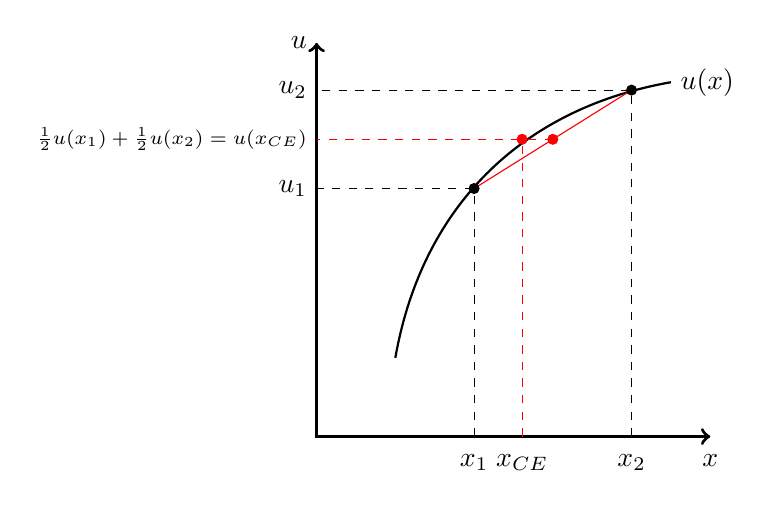
\begin{tikzpicture}[scale = 0.5]
			\draw[very thick,<->] (0,10)--(0,0)--(10,0);
			
			\draw[thick] (2,2) to[out=80,in=190] (9,9);
			
			\node[below] at (10,-0.2) {$x$};
			\node[left] at (0,10) {$u$};
			\node[right] at (9,9) {$u(x)$};
			\node[below] at (4,-0.2) {$x_1$};
			\node[below] at (8,-0.2) {$x_2$};
			\node[below] at (5.22,-0.2) {$x_{CE}$};
			\draw[dashed] (4,0)--(4,6.3)--(0,6.3);
			\draw[dashed] (8,0)--(8,8.8)--(0,8.8);
			\draw[red,dashed] (6,7.55)--(0,7.55);
			\draw[red,dashed] (5.22,0)--(5.22,7.55);
			\node[left] at (0,6.3) {$u_1$};
			\node[left] at (0,8.8) {$u_2$};
			\node[left] at (0,7.55) {\scriptsize $\frac{1}{2}u(x_1) + \frac{1}{2}u(x_2) = u(x_{CE})$};
			\draw[red] (4,6.3)--(8,8.8);
			
			\fill[black] (4,6.3) circle(4pt);
			\fill[black] (8,8.8) circle(4pt);
			\fill[red] (6,7.55) circle(4pt);
			\fill[red] (5.22,7.55) circle(4pt);
		\end{tikzpicture}
		\caption{Risk-Averse Certainty Equivalent}
		\label{fig:risk_averse_ce}
	\end{figure}
\end{remark}

The certainty equivalent allows you to evaluate any lottery in the world of outcomes by which the lottery is realized -- often, the dollar amount between certainty and lottery. For a risk-averse expected utility maximizer, if they have a continuous utility function, it will always be the case that by the Intermediate Value Theorem,
\[
u\parl \sum_{i=1}^N p_ix_i\parr \ge \sum_{i=1}^n p_i u(x_i) \Longrightarrow \exists x_{CE} \st u(x_{CE}) = \sum_{i=1}^n p_i u(x_i)
\]

\begin{remark}
	Note that in the continuous case, we have that 
	\[
	\text{Expected Value} = \int_\reals x dF(x) \qquad \text{ and } \qquad\text{Expected Utility} = \int_\reals u(x) dF(x)
	\]
\end{remark}

\subsection{Insurance}

\begin{example}
	Insurance. Let's assume that there are two possible losses, against which the decision maker can buy insurance. The losses are:
	
	\begin{table}[H]
		\centering
		\begin{tabular}{|c|c|c|c|c|}
			\hline 
			Outcome & Payoff & Probability & Price & How Much Purchased \\
			\hline 
			Loss 1 & $w - L_1$ & $p_1$ & $q_1$ & $\pi_1$ \\
			\hline 
			Loss 2 & $w - L_2$ & $p_2$ & $q_2$ & $\pi_2$ \\
			\hline
			No Loss & $w$ & $1 - p_1 - p_2$ & -- & -- \\
			\hline
		\end{tabular}
	\end{table}
	We have that the attained wealth in each scenario is:
	\begin{align*}
		\text{Loss 1} &: w - L_1 - q_1\pi_1 - q_2\pi_2 + \pi_1 \\
		\text{Loss 2} &: w - L_2 - q_1\pi_1 - q_2\pi_2 + \pi_2 \\
		\text{No Loss} &: w - q_1\pi_1 - q_2\pi_2 
	\end{align*}
	So we are solving the problem
	\[
	\max_{\pi_1,\pi_2} p_1 u(w - L_1 - q_1\pi_1 - q_2\pi_2 + \pi_1) + p_2 u( w - L_2 - q_1\pi_1 - q_2\pi_2 + \pi_2)
	\]
	\[
	+ (1-p_1-p_2) u(w - q_1\pi_1 - q_2\pi_2 )
	\]
	The first order conditions are
	\begin{align*}
		0 &= p_1(1-q_1) u'(\cdot_1) + p_2(-q_1) u'(\cdot_2) + (1-p_1-p_2)(-q_1) u'(\cdot_3) &&(\pi_1) \\
		0 &= p_1(-q_2) u'(\cdot_1) + p_2(1-q_2)u'(\cdot_2) + (1-p_1-p_2)(-q_2) u'(\cdot_3) &&(\pi_2)
	\end{align*}
	Combining, we get that
	\[
	\frac{p_1 u'(\cdot_1)}{p_2 u'(\cdot_2)} = \frac{q_1}{q_2}
	\]
\end{example}

\begin{remark}
	This result required assuming that we know all of $u$, $p$, and $w$. That's extremely strong.
\end{remark}

\subsection{Trees and Floods}

\begin{example}
	Trees. You are a farmer deciding where to plant a grape tree. You can choose either the left bank of a river, the right bank of a river, or on a mountain. We will denote the returns as:
	
	\begin{table}[H]
		\centering
		\begin{tabular}{|c|c|c|}
			\hline
			Choice & Returns without flood & Flood Probability\\
			\hline 
			$L$ & $\ell = 200$ & $f_\ell$\\
			\hline
			$R$ & $r = 200$ & $f_r$ \\
			\hline 
			$M$ & $m = 50$ & 0 \\
			\hline 
		\end{tabular}
	\end{table}
\end{example}

\begin{remark}
	If $L$ and $R$ are divisible and the convex combination of their returns dominate $M$, then $M$ is useless.
\end{remark}

\begin{remark}
	Are the floods mutually exclusive? We need to answer this question.
\end{remark}

We'll say that the consumer can invest total wealth of $1$ into the various locations, denoted by $x_\ell, x_r, x_m$. Our expected utility maximization problem is
\[
\max_{x_\ell + x_r + x_m \le 1} \sum_{i \in \{\emptyset,\ell,r,\ell r\}} f_i u(w_i) \qquad \text{ where } w_{\emptyset} = x_mm
\]
Let's assume that the floods are independent. Then we have that
\begin{align*}
	\prob\{\text{no flood}\} &= (1-f_\ell)(1-f_r) &&\Longrightarrow w = x_\ell \ell + x_r r + x_mm \\
	\prob\{\ell\text{ flood}\} &= f_\ell(1-f_r) &&\Longrightarrow w =  x_r r + x_mm \\
	\prob\{r\text{ flood}\} &= (1-f_\ell)f_r &&\Longrightarrow w = x_\ell \ell + x_mm \\
	\prob\{\ell r\text{ flood}\} &= f_\ell f_r &&\Longrightarrow w =  x_mm
\end{align*}
Suppose that preferences are CARA, so $u(x) = -\exp(-\gamma x)$ for some $\gamma$. Our maximization problem becomes
\begin{align*}
	\max_{x_\ell + x_r + x_m \le 1}& -(1-f_\ell)(1-f_r)\exp(-\gamma (x_\ell \ell + x_r r + x_mm)) \\
	&-  f_\ell(1-f_r)\exp(-\gamma (x_r r + x_mm)) - (1-f_\ell)f_r \exp(-\gamma ( x_\ell \ell + x_mm )) \\
	&-  f_\ell f_r \exp(-\gamma x_mm) 
\end{align*}
Note that since the utility function is increasing, the constraint will hold with equality. We can substitute, and the problem becomes
\[
-f_\ell \barl f_r \exp(-\gamma (1-x_r - x_\ell)m)  + (1-f_r)\exp(-\gamma (x_r r + (1-x_r - x_\ell)m))\barr
\]
\[
-(1-f_\ell) \barl (1-f_r)\exp(-\gamma (x_\ell \ell + x_r r + (1-x_r - x_\ell)m)) + f_r \exp(-\gamma ( x_\ell \ell + (1-x_r - x_\ell)m ))\barr
\]
Note that this is multiplicatively separable into terms with $x_\ell$ and $x_r$. We can rewrite the problem as
\[
	\Big[-f_\ell \exp(\gamma x_\ell m)  -(1-f_\ell) \exp(-\gamma x_\ell (\ell - m))\Big]\Big[f_r \exp(-\gamma (1-x_r)m)  +(1-f_r)\exp(-\gamma (x_r r + (1-x_r)m)) \Big] 
\]

\begin{remark}
	This is a fairly deep result. We can think of it as essentially, since the events are independent, ignoring whether or not the left (or right) bank will flood when considering the optimal amount to invest in the other bank. This result generalizes, and is extremely nice for the purposes of modeling. It means that we don't need to consider, for example, the probability that a random event in New York will happen or not when modeling something in California, as long as the two aren't dependent.
\end{remark}

\subsection{Miscellanea}

\paragraph{Some Nice Intuition.}


\begin{definition}
	The \blue{equity premium} is the gain in expected value a risky asset gives over a safe asset. This doesn't \emph{need} to hold, but in a world where we generally think people are risk-averse, nobody would be interested in an asset that had both higher risk and less return than a safe asset. 
\end{definition}

\begin{remark}
	If two events are (perfectly) correlated, then one of them is irrelevant. Prof. Barseghyan provided this intuition: If one event is whether the Kansas City Chiefs win and another is whether people drink in Kansas City, owning one implicitly means you own the other. Moreover, if someone benefits from one asset implicitly, they should bet against it to hedge. A Ford employee with stock options should, with their own money, invest in Tesla, if they assume it's a zero-sum game.
\end{remark}


\paragraph{Some Definitions.} 

\begin{definition}
	\blue{Loss aversion} is a behavioral result where someone will refuse a single lottery but accept multiple independent draws of the lottery. This is intuitively rational, but doesn't actually make sense in expected utility theory.
\end{definition}
\begin{definition}
	\blue{Prospect Theory} is another explanation for a behavioral result. Prof. Blume talked about it a bit, but think about it as reweighting probabilities before evaluating expected utility.
\end{definition}

\paragraph{Some Formality.} (From Stanford E202 Uncertainty Notes, by Ilya Segal and Ravi Jagadeesan)

\begin{remark}
	I'm honestly not sure how much of this will be relevant, and I'm unsure if any of it is examinable. However, I appreciate rigor when it's available, so I figured I'd include this for completeness and as a reference if nothing else.
\end{remark}

\begin{definition}
	A decision maker is \blue{(strictly) risk-averse} if for any non-degenerate lottery $F$ with expected value $E_F$, the decision maker (strictly) prefers $\delta_{E_F}$, the degenerate lottery that pays $E_F$ with probability 1, to $F$.
\end{definition}

\begin{proposition}
	A decision maker is risk-averse if and only if her Bernoulli utility function is concave.
\end{proposition}

\begin{definition}
	The \blue{certainty equivalent} $c(F,u)$ is the amount of dollars such that
	\[
	u(c(F,u)) = \int u(x)dF(x)
	\]
	The \blue{risk premium} of lottery $F$ for decision maker $u$ is the difference $\expect_F[X] - c(F,u)$.
\end{definition}

\begin{definition}
	For a twice-differentiable Bernoulli utility function $u(\cdot)$, the \blue{Arrow-Pratt Coefficient of Absolute Risk Aversion} at $x$ is $A(x) = -\frac{u''(x)}{u(x)}$
\end{definition}

\begin{proposition}
	The following are equivalent for decision makers $u$ and $v$:
	\begin{itemize}
		\item[(i)] $u$ is more risk averse than $v$
		\item[(ii)] For every lottery $F$, $c(F,u) \le c(F,v)$
		\item[(iii)] There exists an increasing concave function $g$ such that $u = g \circ v$
		\item[(iv)] $\frac{u'(x)}{v'(x)}$ is nondecreasing in $x$
		\item[(v)] For every $x$, $A(x,u) \ge A(x,v)$
		\item[(vi)] Whenever $u$ weakly prefers a lottery $F$ to a certain outcome $\delta_x$, then $v$ does as well
	\end{itemize}
\end{proposition}

\begin{definition}
	The Bernoulli utility function $u(\cdot)$ has \blue{decreasing (constant, increasing) absolute risk aversion} if $A(x,u)$ is a decreasing (constant, increasing) function of $x$.
\end{definition}

\begin{definition}
	For a Bernoulli utility function $u(\cdot)$, the \blue{coefficient of relative risk aversion} at $x$ is $R(x,u) = -x \frac{u''(x)}{u'(x)} \equiv xA(x,u)$. $u$ has \blue{decreasing (constant, increasing) relative risk aversion} if $R(x,u)$ is a decreasing (constant, increasing) function of $x$.
\end{definition}

\begin{definition}
	The distribution $G$ \blue{first order stochastically dominates (FOSD)} the distribution $F$ if for every nondecreasing function $u: \reals \to \reals$, $\int u(x)dG(x) \ge \int u(x)dF(x)$. 
\end{definition}
\begin{proposition}
	The distribution $G$ first order stochastically dominates the distribution $F$ if and only if for every $x$, $G(x) \le F(x)$.
\end{proposition}

\begin{definition}
	Suppose that distributions $G$ and $F$ with common support have densities $g$ and $f$ respectively. We say that $G$ \blue{dominates $F$ in the likelihood ratio order} if $\frac{g(x)}{f(x)}$ is nondecreasing in $x$.
\end{definition}
\begin{definition}
	$G$ \blue{conditionally first order stochastically dominates} $F$ if the CDFs conditional on any (positive-measure Borel) set $A \subseteq \reals$ satisfy $G(x \mid A) \le F(x \mid A)$ for all $x$
\end{definition}

\begin{proposition}
	$G$ dominates $F$ in the likelihood ratio order if and only if $G$ conditionally first order stochastically dominates $F$.
\end{proposition}

\begin{definition}
	Consider two distributions $G$ and $F$ with the same mean. We say that $G$ \blue{second-order stochastically dominates (SOSD)} $F$ if for every concave function $u: \reals \to \reals$, $\int u(x)dG(x) \ge \int u(x) dF(x)$.
\end{definition}
\begin{proposition}
	Consider two distributions $G$ and $F$ with the same mean. $G$ second order stochastically dominates $F$ if and only if for every $x$,
	\[
	\int_{-\infty}^x G(y) dy \le \int_{-\infty}^x F(y)dy
	\]
\end{proposition}

\begin{remark}
	From \href{https://www.sciencedirect.com/science/article/abs/pii/0022053170900384}{Rothschild and Stiglitz (1970)}, there's a really nice intuition for this. We can think of adding random, mean zero noise to a distribution. This is called a `mean preserving spread' as the resulting distribution will have the same mean but will be more spread out. Any distribution first order stochastically dominates its mean preserving spreads. To see why, consider a lottery that pays \$2 or \$0 with probability $1/2$ each. Now consider a lottery that pays \$3 or \$-1 with probability $1/2$ each. The second is a mean-preserving spread of the first, but clearly a risk-averse person would prefer the first to the second. To prove this in general is a fairly straightforward application of Jensen's Inequality! It's fun.
\end{remark}

\begin{remark}
	Another equivalent definition of SOSD, without restricting $G$ and $F$ from having the same mean is that any von Neumann-Morgenstern decision maker with nondecreasing and (not necessarily strictly) concave Bernoulli utility prefers $G$ to $F$. You can probably show fairly easily that this is equivalent to the definition in Proposition 5.5. However, can you explain why we no longer care about the means being equal? What would happen if the means were not equal?
\end{remark}

\begin{proposition}
	If decision-maker $u$ is less risk-averse than decision maker $v$, then $u$ will optimally choose to take more risk than $v$ for any CDF $G(\cdot)$.
\end{proposition}



























\newpage
\section{Information Theory (Battaglini)}\label{sec:battaglini}

\subsection{Asymmetric Information}

\begin{definition}
	We say that we have \blue{complete information} if all agents know all of the relevant information. We say that information is \blue{incomplete} otherwise. We have two types of incomplete information:
	\begin{itemize}
		\item[(i)] \blue{Symmetric incomplete information}: some variables are unknown, but no privileged information
		\item[(ii)] \blue{Asymmetric incomplete information}: some players have more information than others
	\end{itemize}
\end{definition}

\begin{remark}
	We have two broad categories of asymmetric information problems: (i) \blue{adverse selection}, when the asymmetric information concerns the characteristics of the agents (think insurance, lending, selling, etc); and (ii) \blue{moral hazard} when the information concerns the action of some character (think work relations, also insurance, also lending, etc).
\end{remark}

\begin{model}
	\red{(Lemons)} (from \href{https://www.jstor.org/stable/1879431}{Akerlof (1970)}). Consider a labor market in which a worker produces $\theta$ units. $\theta$ has distribution $F(\theta)$ in $[\underline{\theta},\overline{\theta}]$, with $0 < \underline{\theta} < \overline{\theta} < \infty$. Firms hire workers to produce the good and sell it in a competitive market at price $p = 1$. The number of workers is $N$, and firms are risk-neutral. Workers have a reservation value for their time $r(\theta)$, which can be thought of as unemployment insurance, or the value of going to school, or whatever. Employed workers receive a wage, which may or may not depend on $\theta$.
\end{model}

\paragraph{Complete Information.} In a competitive equilibrium with complete information, all workers with $r(\theta) < \theta$ are employed. $w(\theta) = \theta$ for all employed workers, and $w(\theta) < \theta$ for the unemployed. Note that this market outcome is Pareto optimal: it is not possible to make any worker strictly better off without making some agent strictly worse off. Aggregate surplus in this model is:
\[
W\opt = \int_{\underline{\theta}}^{\overline{\theta}} N \barl \ones_{\theta} \cdot \theta + (1 - \ones_\theta) r(\theta)\barr dF(\theta)
\]
where $\ones_\theta = 1$ if $r(\theta) < \theta$ and 0 otherwise.

\paragraph{Asymmetric Information.} Since worker types are unobservable, there will only be one market here, with price $w$. Supply in this market is $\Theta(w)\coloneqq \{\theta : r(\theta) < w\}$, so $S(w) = F(r^{-1}(w))$. For simplicity, let's assume that indifferent workers will choose to work. Demand is:
\[
D(w) = \begin{cases} 0 & \expect \theta < w \\ [0,\infty] & \expect \theta = w \\ \infty & \expect \theta > w \end{cases}
\]
It is clear that $S(w) = D(w)$ only when $\expect \theta = w$. At the same time, $\expect\theta$ must be consistent with supply, so we must have that $w = \expect\barl\theta : r(\theta) \le w\barr$. This condition is called \blue{rational expectations}.

\begin{definition}
	Ina. competitive market model with unobservable worker's productivity, a \blue{competitive equilibrium} is a wage rate $w\opt$ and a set of workers $\Theta\opt$ such that
	\[
	\Theta\opt = \{\theta : r(w) \le w\} \quad \text{ and } \quad w\opt = \expect\barl \theta : \theta \in \Theta\opt\barr 
	\]
\end{definition}

\begin{remark}
	The rational expectation requirement is well-defined only if $\Theta\opt$ is non-empty. If $\Theta\opt$ is an empty set, we need to specify off-path beliefs, since the firms expect no supply of labor. For now, we have the following, which is as good as anything else:
\end{remark}
\begin{assumption}
	If $\Theta\opt = \emptyset$, then $w\opt = \expect \theta$, the unconditional expectation.
\end{assumption}

\begin{remark}
	In general, with imperfect information, a competitive equilibrium is Pareto inefficient. 
\end{remark}

\begin{example}
	To see this point, assume $r(\theta) = r$ for some constant. The Pareto optimal allocation requires that all workers with $\theta > r$ to work, and all types with $\theta < r$ to not work. But this is impossibly in a competitive equilibrium: if $w > r$, everyone works, and if $w < r$, nobody works. If $w = r$, the types are indifferent, but there's no reason they should sort the way we want. The problem is that firms are unable to distinguish types, so there's no way to sort the workers.
\end{example}


\begin{example}
	(Adverse Selection and Market Unraveling) We now consider the more realistic case where $r(\theta)$ is increasing in $\theta$. For simplicity, we assume that $r(\theta) \le \theta$ for all $\theta$, so it is efficient to have full employment. Further, we assume that $r(\theta)$ is \emph{strictly} increasing in $\theta$. Now we have that $\expect[\theta : r(\theta) \le w]$ is continuous in $w$, as long as $F$ has a density $f$, and is increasing in $w$.
	
	Note some implications: (i) $\expect[\theta : r(\theta) \le r(\underline{\theta})] = \underline{\theta} \ge r(\underline{\theta})$, and (ii) $\expect[\theta : r(\theta) \le r(\overline{\theta})] = \expect \theta < \overline{\theta}$. Thus, we have Figure~\ref{fig:lemon_one_equilibrium}, where $\expect[\theta : r(\theta) \le w]$ is above the $45^\circ$ line at $w = r(\underline{\theta})$, and below at $w = r(\overline{\theta})$. 
	\begin{figure}[H]
		\centering
		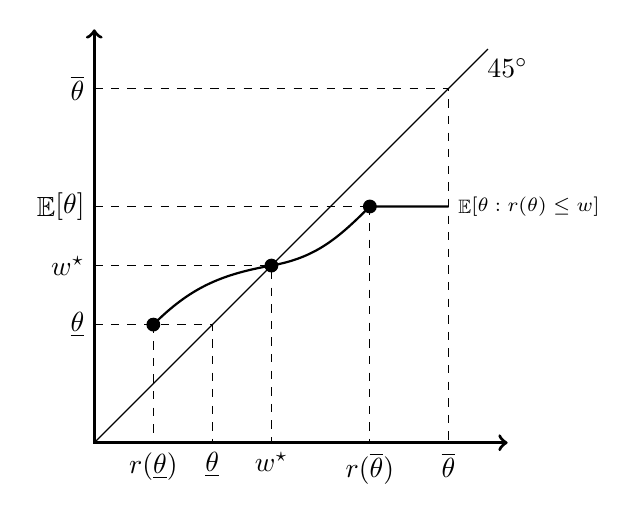
\begin{tikzpicture}[scale=0.5]
    		\draw[very thick,<->] (10.5,0)--(0,0)--(0,10.5);
    		\draw[] (0,0)--(10,10);
 			\node[below] at (10.5,10) {$45^\circ$};   		
    		\draw[dashed] (0,9)--(9,9)--(9,0);
    		\node[left] at (0,9) {$\overline{\theta}$};
    		\node[below] at (9,0) {$\overline{\theta}$};
    		\node[below] at (1.5,0) {$r(\underline{\theta})$};
			\node[below] at (3,0) {$\underline{\theta}$};
			\node[below] at (4.5,0) {$w\opt$};
			\node[below] at (7,0) {$r(\overline{\theta})$};
			\node[left] at (0,6) {$\expect[\theta]$};
			\node[left] at (0,4.5) {$w\opt$};
			\node[left] at (0,3) {$\underline{\theta}$};
			
			\draw[dashed] (0,3)--(3,3)--(3,0);
			\draw[dashed] (0,4.5)--(4.5,4.5)--(4.5,0);
			\draw[dashed] (1.5,3)--(1.5,0);
			\draw[dashed] (0,6)--(9,6);
			\draw[dashed] (7,6)--(7,0);
			
			\draw[thick] (1.5,3) to[out=45, in=190] (4.5,4.5) to[out=10,in=225] (7,6) -- (9,6);
			
			\fill[black] (1.5,3) circle (5pt);
			\fill[black] (4.5,4.5) circle (5pt);
			\fill[black] (7,6) circle (5pt);
			
			\node[right] at (9,6) {\scriptsize $\expect[\theta : r(\theta) \le w]$};
		\end{tikzpicture}
		\caption{Single Equilibrium}
		\label{fig:lemon_one_equilibrium}
	\end{figure}
	
	We must have at least one $w\opt \in (\underline{\theta},\overline{\theta})$ such that $w\opt = \expect[\theta : r(\theta) \le w\opt]$, by Kakutani's Fixed Point Theorem. 
	
	This characterization immediately shows that the equilibrium is inefficient. It would be optimal to have all types employed, but only types $\theta \le r^{-1}(w\opt) < \overline{\theta}$ are employed here. 
\end{example}

\begin{remark}
	We may have multiple equilibria. See Figure~\ref{fig:lemon_multiple_equilibria} for an illustration. If we have multiple equilibria, they can be Pareto ranked -- recall that all profits are zero, but workers do better as $w\opt$ increases.
\end{remark}

\begin{figure}[H]
		\centering
		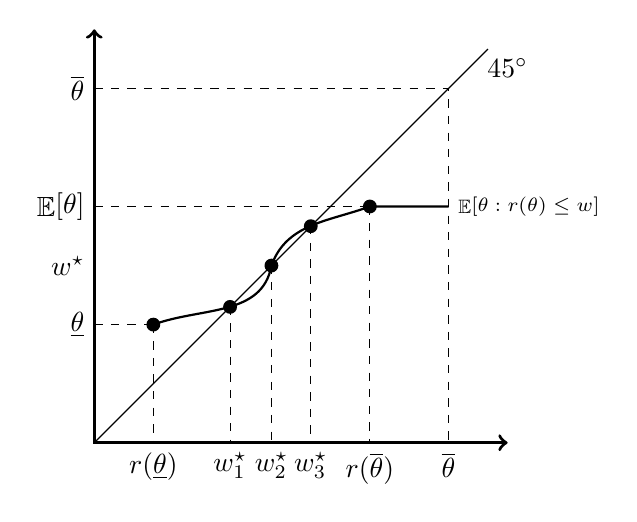
\begin{tikzpicture}[scale=0.5]
    		\draw[very thick,<->] (10.5,0)--(0,0)--(0,10.5);
    		\draw[] (0,0)--(10,10);
 			\node[below] at (10.5,10) {$45^\circ$};   		
    		\draw[dashed] (0,9)--(9,9)--(9,0);
    		\node[left] at (0,9) {$\overline{\theta}$};
    		\node[below] at (9,0) {$\overline{\theta}$};
    		\node[below] at (1.5,0) {$r(\underline{\theta})$};
			\node[below] at (7,0) {$r(\overline{\theta})$};
			\node[left] at (0,6) {$\expect[\theta]$};
			\node[left] at (0,4.5) {$w\opt$};
			\node[left] at (0,3) {$\underline{\theta}$};
			\node[below] at (3.45,0) {$w\opt_1$};
			\node[below] at (4.5,0) {$w\opt_2$};
			\node[below] at (5.5,0) {$w\opt_3$};
			
			\draw[dashed] (0,3)--(1.5,3);

			\draw[dashed] (1.5,3)--(1.5,0);
			\draw[dashed] (0,6)--(9,6);
			\draw[dashed] (7,6)--(7,0);
			\draw[dashed] (3.45,3.45)--(3.45,0);
			\draw[dashed] (4.5,4.5)--(4.5,0);
			\draw[dashed] (5.5,5.5)--(5.5,0);
			
			\draw[thick] (1.5,3) to[out=20, in=-100] (4.5,4.5) to[out=70,in=200] (7,6) -- (9,6);
			
			\fill[black] (1.5,3) circle (5pt);
			\fill[black] (4.5,4.5) circle (5pt);
			\fill[black] (7,6) circle (5pt);
			\fill[black] (3.45,3.45) circle (5pt);
			\fill[black] (5.5,5.5) circle (5pt);
			
			\node[right] at (9,6) {\scriptsize $\expect[\theta : r(\theta) \le w]$};
		\end{tikzpicture}
		\caption{Multiple Equilibria}
		\label{fig:lemon_multiple_equilibria}
	\end{figure}

\begin{remark}
	The classic point made by Akerlof is that the market may totally collapse. See the following example.
\end{remark}

\begin{example}
	Assume that $r(\theta) = \alpha \theta$ for some $\alpha < 1$, and that $\theta \sim U[0,2]$. We have that
	\[
	\expect[\theta : r(\theta) \le w] = \expect[\theta : \alpha \theta \le w] = \expect\barl\theta : \theta \le \frac{w}{\alpha}\barr = \frac{w}{2\alpha}
	\]
	In this case, when $\alpha > \frac{1}{2}$, the market collapses to zero. See Figure~\ref{fig:lemon_collapse}.
	
	\begin{figure}[ht]
		\centering
		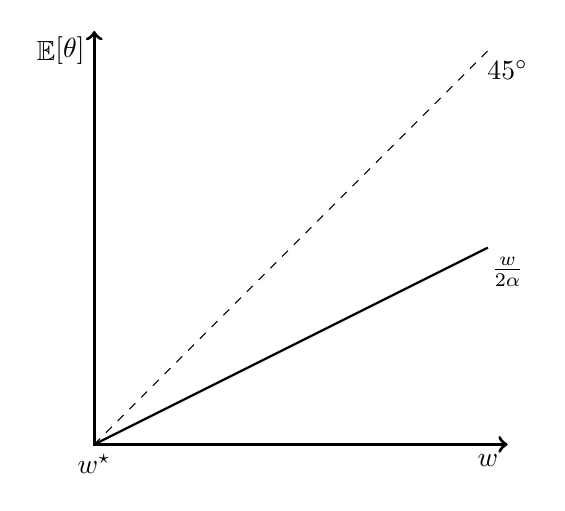
\begin{tikzpicture}[scale = 0.5]
			\draw[<->,very thick] (10.5,0)--(0,0)--(0,10.5);
			
			\draw[dashed] (0,0)--(10,10);
			\draw[thick] (0,0)--(10,5);
			\node[below] at (10,0) {$w$};
			\node[left] at (0,10) {$\expect[\theta]$};
			\node[below] at (10.5,10) {$45^\circ$};
			\node[below] at (10.5,5) {$\frac{w}{2\alpha}$};
			\node[below] at (0,0) {$w\opt$};
		\end{tikzpicture}
		\caption{Collapse In the Market for Lemons}
		\label{fig:lemon_collapse}
	\end{figure}
\end{example}

\begin{question}
	Could this be fixed with public intervention? A case is possible where there are multiple equilibria. In this case, the government could shift the equilibrium to the maximum equilibrium wage. 
	
	Could the government do better than that? If they could see the types, but that's implausible.
\end{question}
\begin{definition}
	A \blue{Constrained Pareto Optimum} is a Pareto Optimum achievable by a planner with no informational advantage. 
\end{definition}
Is there a constrained Pareto optimum that is better than the competitive equilibrium? The answer is no.

\begin{example}
	The planner chooses $w_e$ and $w_u$ (employed and unemployed). Given this, all workers of type $\theta \le \hat{\theta}$ will work, where $w_u + r(\hat{\theta}) = w_e$. So the government can only choose $\hat{\theta}$, $w_e$, and $w_u$ such that the budget balance is satisfied:
	\[
	w_e F(\hat{\theta}) + w_u [ 1 - F(\hat{\theta})] \le \int \theta dF(\theta)
	\]
	Substituting, we get that
	\begin{align*}
		w_u(\hat{\theta}) &= \int \theta dF(\theta) - r(\hat{\theta})F(\hat{\theta}) \\
		w_e(\hat{\theta}) &= \int \theta dF(\theta) - r(\hat{\theta})[1-F(\hat{\theta})]
	\end{align*}
	meaning that
	\begin{align*}
		w_u(\hat{\theta}) &=F(\hat{\theta}) \barl \expect [\theta : \theta \le \hat{\theta}] - r(\hat{\theta})\barr \\
		w_e(\hat{\theta}) &= F(\hat{\theta}) \barl \expect [\theta : \theta \le \hat{\theta}] - r(\hat{\theta})\barr + r(\hat{\theta})
	\end{align*}
	Let $\theta\opt$ be the highest type employed in the highest competitive equilibrium, so:
	\[
	r(\theta\opt) \expect[\theta : \theta \le \theta\opt] = w\opt
	\]
	If the government selects $\hat{\theta} = \theta\opt$, we have $w_e(\hat{\theta}) = w\opt$, and $w_u(\hat{\theta}) = 0$. So the outcome is the competitive equilibrium. There are two other possibilities: $\hat{\theta} > \theta\opt$ and $\hat{\theta} < \theta\opt$. If $\hat{\theta} < \theta\opt$, we have that
	\[
	w_e(\hat{\theta}) = F(\hat{\theta}) \barl \expect [\theta : \theta \le \hat{\theta}] - r(\hat{\theta})\barr + r(\hat{\theta})
	\]
	\[
	\qquad\quad< F(\hat{\theta}) \barl \expect [\theta : \theta \le \hat{\theta}] - r(\theta\opt)\barr + r(\theta\opt)
	\]
	since $r(\theta\opt) > r(\hat{\theta})$. We also have that
	\begin{align*}
		w_e(\hat{\theta}) - r(\theta\opt) &\le F(\hat{\theta})\barl \expect[\theta : \theta \le \hat{\theta}] - r(\theta\opt)\barr \\
		&= F(\hat{\theta})\barl \expect[\theta : \theta \le \hat{\theta}] -\expect[\theta : \theta \le \theta\opt]\barr < 0
	\end{align*}
	It follows directly that $w_e(\hat{\theta}) < r(\theta\opt) = w\opt$. Low types were working in the competitive equilibrium for a higher wage, and they are now worse off.
	
	The other case assumes that $\hat{\theta} > \theta\opt$. We must have that $\expect[\theta : r(\theta) \le w] < w$ for all $w \ge w\opt$, otherwise $w\opt$ would not be the highest competitive equilibrium. Since $w\opt = r(\theta\opt)$ and $r(\theta)$ is increasing, $r(\hat{\theta}) > r(\theta\opt) = w\opt$, so
	\[
	\expect\barl \theta : r(\theta) \le r(\hat{\theta})\barr < r(\hat{\theta})
	\]
	for $\hat{\theta} \ge \theta\opt$. So $w_u(\hat{\theta}) = F(\hat{\theta}) \barl \expect[\theta : \theta \le \hat{\theta}] - r(\hat{\theta})\barr \le 0$, implying that the high types that remain unemployed are worse off now.
\end{example}

\subsection{Separating and Pooling Equilibria}

\begin{example}
	One way the market might bypass the information asymmetry is by allowing workers to signal their type. Assume here that there are two types, $0 < \theta_L < \theta_H$, with $\prob\{\theta_H\} = \lambda$. We now assume that workers can get some education $e$. To make the point more striking, education is unproductive. 
	
	The cost of education is $C(e,\theta)$ with (i) the usual technological assumptions, so $C(0,\theta) = 0$, $C_e(e,\theta) > 0$, and $C_{ee}(e,\theta)> 0$; and (ii) we assume that $C_\theta(e,\theta) < 0$ and $C_{e\theta}(e,\theta) < 0$. Note that these are the Single Crossing Property we saw in Math.
	
	Note that now the wage depends on the observable $e$, so the wage is a function $w(e)$. Utility is now
	\[
	U(w,e;\theta) = w(e) - c(e,\theta)
	\]
	We assume that $r(\theta) = 0$, so in a competitive market with no signaling all types are employed at wage $\expect[\theta]$. A \blue{competitive equilibrium with signaling} is now a competitive equilibrium for each $e$, meaning a $\Theta(e)$, $w(e)$ such that
	\[
	w(e) = \expect[\theta : \theta \in \Theta(e)] \qquad \text{and} \qquad \Theta(e) = \{\theta : e \in \argmax_e U(w(e),e;\theta)\}
	\]
	We can plot indifference curves in the $(w,e)$ space. Indifference curves for high and low types will typically cross only once, and the indifference curves for high types are less steep, since
	\[
	\frac{\partial w(e)}{\partial e} = C_e(e,\theta) \qquad \text{ and } C_e(e,\theta_H) < C_e(e,\theta_L)
	\]
	This is illustrated in Figure~\ref{fig:indifference_educ}.
	\begin{figure}[H]
		\centering
		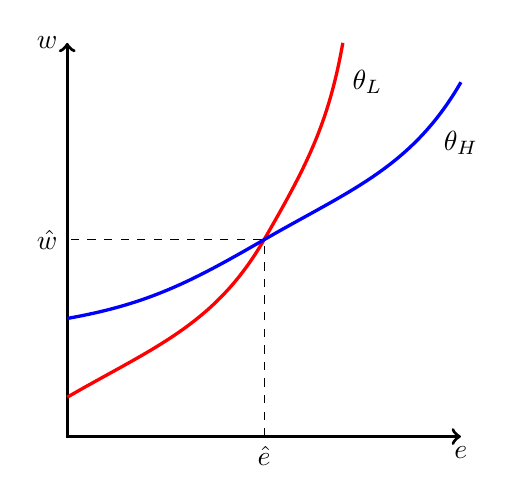
\begin{tikzpicture}[scale=0.5]
			\draw[<->,very thick] (10,0)--(0,0)--(0,10);
			\node[below] at (10,0) {$e$};
			\node[left] at (0,10) {$w$};
			
			
			\node[below] at (5,0) {$\hat{e}$};
			\node[left] at (0,5) {$\hat{w}$};
			\draw[dashed] (5,0)--(5,5)--(0,5);
			\draw[very thick, red] (0,1) to[out=30,in=240] (5,5) to[out=60,in=260] (7,10);
			\draw[very thick,blue] (0,3) to[out=10,in=210] (5,5) to[out=30,in=240] (10,9);
			
			\node[below] at (10,8) {$\theta_H$};
			\node[right] at (7,9) {$\theta_L$};
		\end{tikzpicture}
		\caption{Indifference Curves for High and Low Types}
		\label{fig:indifference_educ}
	\end{figure}
	The wage function can be represented as
	\[
	w(e) = \mu(e)\theta_H + (1-\mu(e))\theta_L
	\]
	where $\mu(e)$ is the posterior probability of observing a high type. This function is illustrated in Figure~\ref{fig:wage_fn_educ}.

	\begin{figure}[H]
		\centering
		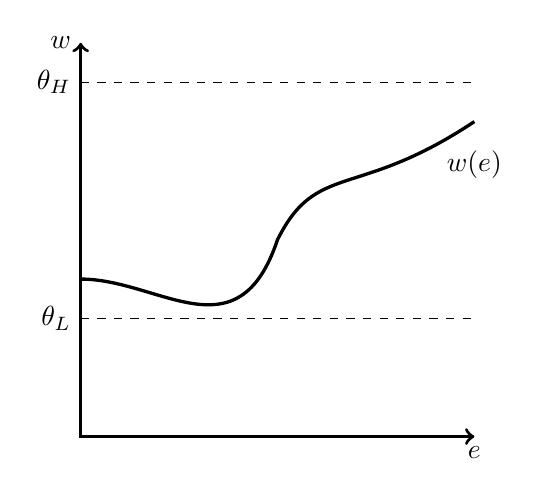
\begin{tikzpicture}[scale=0.5]
			\draw[<->,very thick] (10,0)--(0,0)--(0,10);
			\node[below] at (10,0) {$e$};
			\node[left] at (0,10) {$w$};
			
			\node[left] at (0,3) {$\theta_L$};
			\node[left] at (0,9) {$\theta_H$};
			\draw[dashed] (0,3)--(10,3);
			\draw[dashed] (0,9)--(10,9);
			
			\draw[very thick,domain=0:10,smooth] (0,4) .. controls (2,4) and (4,2) .. (5,5) .. controls (6,7) and (7,6) .. (10,8);
			\node[below] at (10,7.5) {$w(e)$};
		\end{tikzpicture}
		\caption{Wage Function on Education}
		\label{fig:wage_fn_educ}
	\end{figure}
	\begin{remark}
		We haven't explicitly discussed Bayesian posterior probabilities before. These are directly derived from Bayes' Rule. Formally, in this example, we have that 
		\[
		\mu(e) = \prob\{\theta = \theta_H | e = 1\} = \frac{\prob\{e = 1 | \theta = \theta_H\}}{\prob\{e = 1 | \theta = \theta_H\} + \prob\{e = 1 | \theta = \theta_L\}}
		\]
	\end{remark}
\end{example}

\begin{definition}
	In a \blue{separating equilibrium}, the two types choose different actions: $e\opt(\theta_H) \ne e\opt(\theta_L)$. This immediately implies two facts: (i) In a separating equilibrium, we must have that $w(e\opt(\theta_H)) = \theta_H$ and $w(e\opt(\theta_L)) = \theta_L$; and (ii) we must have that $e\opt(\theta_L) = 0$. Why is this? The low type gets no benefit from $e\opt(\theta_L)$, so by choosing $e\opt(\theta_L) = 0$, she gets the same wage and lower costs. 
\end{definition}

Starting from here, we will construct a separating equilibrium. We need that $e\opt(\theta_L) = 0$ and $e\opt(\theta_H)$ such that
\[
U(w(e\opt(\theta_H)),e\opt(\theta_H); \theta_H) \ge U(w(e),e;\theta_H) \forall e
\]
\[
U(w(e\opt(\theta_L)),e\opt(\theta_L); \theta_L) \ge U(w(e),e;\theta_L) \forall e
\]
these are called our \blue{incentive compatability constraints}, and they guarantee that neither high nor low types are incentivized to deviate from what we think they should do.



An example of this equilibrium is illustrated in Figure~\ref{fig:separating_eq_educ}.

	\begin{figure}[H]
		\centering
		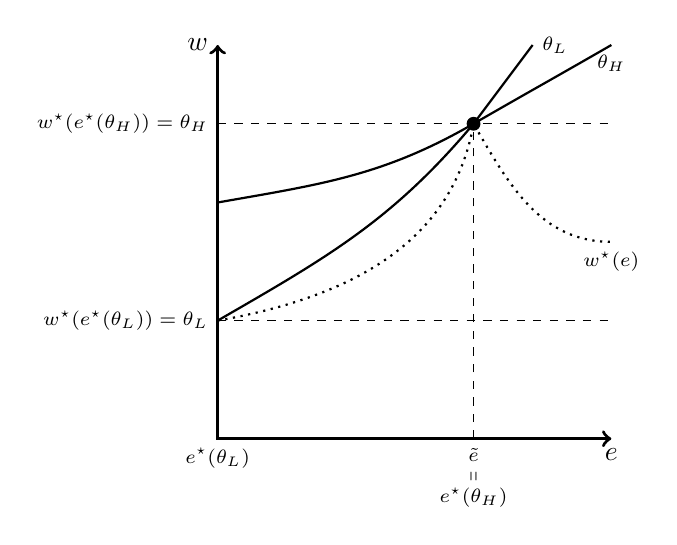
\begin{tikzpicture}[scale=0.5]
			\draw[<->,very thick] (10,0)--(0,0)--(0,10);
			\node[below] at (10,0) {$e$};
			\node[left] at (0,10) {$w$};
		
		
			\node[left] at (0,3) {\scriptsize $w\opt(e\opt(\theta_L))=\theta_L$};
			\node[left] at (0,8) {\scriptsize $w\opt(e\opt(\theta_H))=\theta_H$};
			% Curves
    \draw[thick] (0,6) to[out=10, in=210] (6.5,8) to[out=30,in=210] (10,10); % Theta_H curve
    \draw[thick] (0,3) to[out=30, in=230] (6.5,8) --(8,10); % Theta_L curve

    \draw[dashed] (0,3) -- (10,3);
    \node[below] at (6.5,0) {\scriptsize $\tilde{e}$};

    % Additional curve
    \draw[thick, dotted] (0,3) to[out=10, in=260] (6.5,8) to[out=-60,in=180] (10,5);
    \node[below] at (10,5) {\scriptsize$w\opt(e)$};

    % Dashed lines for intersections
    \draw[dashed] (0,8) -- (10,8); % Horizontal line
    \draw[dashed] (6.5,0) -- (6.5,8); % Theta_H horizontal intersection

    % Labels for intersections
    \node[below] at (0,0) {\scriptsize $e\opt(\theta_L)$};
    \node[below] at (6.5,-1) {\scriptsize $e\opt(\theta_H)$};
    \node[below] at (6.5,-0.5) {\scriptsize $\shortparallel$};
    \node[below] at (10,10) {\scriptsize $\theta_H$};
    \node[right] at (8,10) {\scriptsize $\theta_L$};
    \fill[black] (6.5,8) circle(5pt);
		\end{tikzpicture}
		\caption{A Separating Equilibrium}
		\label{fig:separating_eq_educ}
	\end{figure}

Note that here we have that (i) $e\opt(\theta_L) = 0$, (ii) $U(w(e\opt(\theta_L)),e\opt(\theta_L);\theta_L) = U(w(e\opt(\theta_H)),e\opt(\theta_H);\theta_L)$, and (iii) $U(w(e\opt(\theta_H)),e\opt(\theta_H);\theta_H) \ge U(w(e\opt(\theta_L)),e\opt(\theta_L);\theta_H)$. 

\begin{remark}
	We need here to specify wages for all $e$, even though only two will be chosen. This is because $w(e) = \mu(e)\theta_H + (1-\mu(e))\theta_L$, meaning that
	\[
	\mu(e)=\frac{w(e)-\theta_L}{\theta_H-\theta_L}
	\]
\end{remark}

\begin{remark}
	We can have other equilibria, but (referring back to Figure~\ref{fig:separating_eq_educ}), the educational level for the high type cannot be lower than $\tilde{e}$, otherwise we would violate the incentive compatibility constraint for the low type (they would pay to get the higher wage). The educational level of the high type cannot be higher than $e_1$, otherwise we would violate incentive compatibility for the high type (they would rather not pay and not get hired).
\end{remark}

\begin{remark}
	The equilibria can be Pareto ranked: profits are always zero in a competitive equilibrium, and effort is a net loss, so the lower $e$ the better. 
\end{remark}

\begin{question}
	Are the players better off with signaling? The low type is always worse off -- before signaling, he was hired at $w = \expect[\theta]$, now he is either hired at $w = 0$ or unemployed. The high type may or may not be better off -- before signaling, her utility is $w = \expect[\theta] = U(\expect[\theta],0;\theta_H)$, and with signaling her utility is $U(w(e\opt(\theta_H)),e\opt(\theta_H);\theta_H) = w(e\opt(\theta_H)) - e\opt(\theta_H)$. She may be better off or worse off depending on the expectation of $\theta$ -- which comes entirely from the Bayesian prior $\lambda$.
\end{question}

\begin{definition}
	In a \blue{pooling equilibrium}, the two types choose the same action, so they are indistinguishable: $e\opt(\theta_H) = e\opt(\theta_L) = e\opt$. It follows that $w(e\opt) = \lambda \theta_H + (1-\lambda)\theta_L = \expect[\theta]$. 
\end{definition}

\begin{remark}
	Again in this equilibrium, we need to define the wage for $e \ne e\opt$. We need incentive compatibility again, meaning that for any $e$:
	\[
	U(\expect[\theta],e\opt;\theta_H) \ge U(w(e),e;\theta_H)
	\]
	\[
	U(\expect[\theta],e\opt;\theta_L) \ge U(w(e),e;\theta_L)
	\]
	An example of this equilibrium is illustrated in Figure~\ref{fig:pooling_eq_educ}.
	\begin{figure}[H]
		\centering
		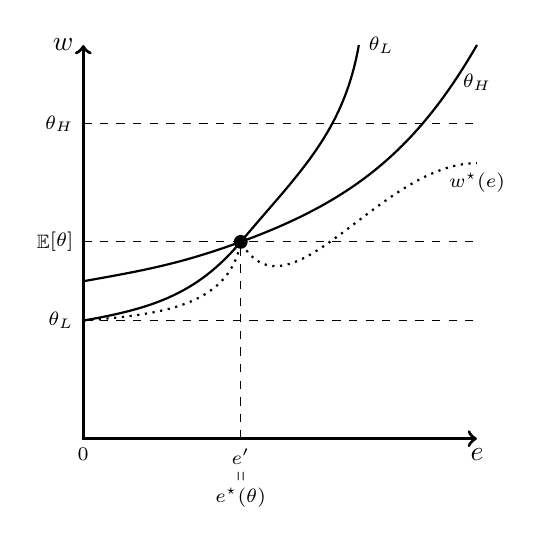
\begin{tikzpicture}[scale=0.5]
			\draw[<->,very thick] (10,0)--(0,0)--(0,10);
			\node[below] at (10,0) {$e$};
			\node[left] at (0,10) {$w$};
		
		
			\node[left] at (0,3) {\scriptsize $\theta_L$};
			\node[left] at (0,8) {\scriptsize $\theta_H$};
			\node[left] at (0,5) {\scriptsize $\expect[\theta]$};
			% Curves
    \draw[thick] (0,4) to[out=10, in=200] (4,5) to[out=20,in=240] (10,10); % Theta_H curve
    \draw[thick] (0,3) to[out=10, in=230] (4,5) to[out=50,in=260](7,10); % Theta_L curve

    \draw[dashed] (0,3) -- (10,3);
    \node[below] at (4,0) {\scriptsize $e'$};

    % Additional curve
    \draw[thick, dotted] (0,3) to[out=5, in=260] (4,5) to[out=-60,in=180] (10,7);
    \node[below] at (10,7) {\scriptsize$w\opt(e)$};

    % Dashed lines for intersections
    \draw[dashed] (0,8) -- (10,8); % Horizontal line
    \draw[dashed] (0,5)--(10,5);
    \draw[dashed] (4,0) -- (4,5); % Theta_H horizontal intersection

    % Labels for intersections
    \node[below] at (0,0) {\scriptsize $0$};
    \node[below] at (4,-1) {\scriptsize $e\opt(\theta)$};
    \node[below] at (4,-0.5) {\scriptsize $\shortparallel$};
    \node[below] at (10,9.5) {\scriptsize $\theta_H$};
    \node[right] at (7,10) {\scriptsize $\theta_L$};
    \fill[black] (4,5) circle(5pt);
			
		\end{tikzpicture}
		\caption{A Pooling Equilibrium}
		\label{fig:pooling_eq_educ}
	\end{figure}
\end{remark}

\begin{remark}
	Multiple levels of effort can be sustained in a pooling equilibrium, as long as there are `punishments' for lower levels of effort. In this way, we can sustain positive effort even for low types.
\end{remark}

\begin{remark}
	The highest level of education corresponds to $U(\expect[\theta],e_1;\theta_L) = U(\theta_L,0;\theta_L) = \theta_L$. Anything higher violates incentive compatibility. The lowest pooling equilibrium is, of course $e = 0$. 
\end{remark}


\subsection{Separating and Pooling Refinements}

\begin{example}
	Consider an $e'$ such that
	\[
	\expect[\theta] - C(e\opt,\theta_L) \ge \theta_H - C(e',\theta_L) \text{ and } \expect[\theta] - C(e\opt,\theta_H) < \theta_H - C(e',\theta_H)
	\]
	where $e\opt$ is a pooling equilibrium. Since a low type is worse off if believed and a high type is better off, a receiver would believe that a deviator is a high type. 
\end{example}
\begin{remark}
	Such a point $e'$ \emph{always exists}. We can conclude that no pooling equilibria exist. To see why, consider that if everyone else is pooling, and you are a low type, you can deviate and be considered the only high type. By doing so, you would attain the highest salary, and do better! Thus, incentive compatibility is \emph{never} satisfied for all low types.
\end{remark}

\begin{example}
	Consider now a separating equilibrium with $e^L = 0$, $e^H$. In such an equilibrium, in order for incentive compatibility to hold, we need that $\theta_H - C(e^H,\theta_H) \ge \theta_L$. Assume that $\theta_H - C(e^H,\theta_L) < \theta_L$. Then if the receiver sees a deviation $e' < e^H$, but still has that $\theta_H - C(e',\theta_L) < \theta_L$, knowing that a high type benefits from being believed and a low type does not, the receiver will assume that the deviator is a high type. 
\end{example}

\begin{remark}
	Such an $e'$ exists in all cases \emph{except} when $e^L = 0$ and $\theta_H - C(e^H ,\theta_L) = \theta_L$. This is the only separating equilibrium that survives refinement. 
\end{remark}

\subsection{Screening Games}

\begin{remark}
	In the previous analysis, informed agents chose education to self-select, and to try and signal their types. If we flipped the game so it's uninformed agents trying to screen the informed agents, then we have screening.
\end{remark}

\begin{model}
	Let's assume the same environment as before: we have two types $0 < \theta_L < \theta_H$, with $\prob\{\theta_H\} = \lambda$, and now assume that $r(\theta) = 0$. We will assume that (unproductive) tasks can be assigned to the agents. These tasks cost effort $C(t,\theta)$ with the same assumptions as before: $C(0,\theta) = 0$, $C_t(t,\theta) > 0$, $C_{tt}(t,\theta) > 0$, $C_\theta(t,\theta) < 0$, and $C_{t\theta}(t,\theta)< 0$.  
\end{model}

\begin{definition}
	A \blue{contract} is a pair $(t,w(t))$, where $t$ is a task and $w(t)$ is the associated wage if that task is completed. 
\end{definition}

Let $\Theta(t) \coloneqq \{\theta : t \in \argmax_t u(w(t),t;\theta)\}$ be the set of all agents who complete a task $t$. 

\begin{definition}
	A family of contracts $(t,w(t))_t$ is a \blue{competitive equilibrium} if (i) $w(t) = \expect[\theta : \theta \in \Theta(t)]$, and (ii) profits are zero for all contracts $(t,w(t))$. 
\end{definition}

\begin{remark}
	With observable types, $(t,w(t,\theta)) = (0,\theta)$. With unobservable types, we have three cases: perfectly separating equilibria, pooling equilibria, and partially separating equilibria. We will not really study the third.
\end{remark}

Our first result is that no pooling equilibrium can exist. See Figure~\ref{fig:screening_pooling}. The high type would always deviate from $(w^p,t^p)$ to $(\tilde{w},\tilde{t})$, and this necessarily follows from the single crossing assumptions.

\begin{figure}[H]
	\centering
		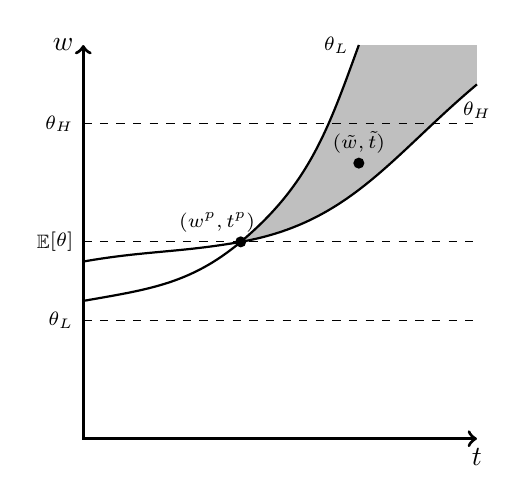
\begin{tikzpicture}[scale=0.5]
			\draw[<->,very thick] (10,0)--(0,0)--(0,10);
			\node[below] at (10,0) {$t$};
			\node[left] at (0,10) {$w$};
		
		
			\node[left] at (0,3) {\scriptsize $\theta_L$};
			\node[left] at (0,8) {\scriptsize $\theta_H$};
			\node[left] at (0,5) {\scriptsize $\expect[\theta]$};
			
			\draw[dashed] (0,3)--(10,3);
			\draw[dashed] (0,8)--(10,8);
			\draw[dashed] (0,5)--(10,5);
			
			\draw[thick] (0,3.5) to[out=10,in=220] (4,5) to[out=40,in=250] (7,10);
			\draw[thick] (0,4.5) to[out=10,in=190] (4,5) to[out=10,in=220] (10,9);
			\node[below] at (10,8.8) {\scriptsize $\theta_H$};
			\node[left] at (7,10) {\scriptsize $\theta_L$};
			
			\fill[black,nearly transparent] (4,5) to[out=40,in=250] (7,10) --(10,10)--(10,9) to[out=220,in=10] (4,5);
			\fill[black] (4,5) circle(4pt);
			\fill[black] (7,7) circle(4pt);
			\node[above] at (7,7) {\scriptsize $(\tilde{w},\tilde{t})$};
			\node[above] at (3.4,5) {\scriptsize $(w^p,t^p)$};
		\end{tikzpicture}
		\caption{A Potential Pooling Equilibrium}
		\label{fig:screening_pooling}
\end{figure}

Our second result is that if $w_L,t_L,w_H,t_H$ are equilibrium contracts in a separating equilibrium, then $(w_L,t_L) = (\theta_L,0)$ and $(w_H,t_H) = (\theta_H,t\opt_H)$ such that
\[
\theta_H - C(t\opt_H,\theta_L) = \theta_L - C(0,\theta_L)
\]
so that the low type is indifferent between $(w_L,t_L)$ and the contract for the high type. The intuition is in Figure~\ref{fig:screening_separating}. 


\begin{figure}[H]
	\centering
		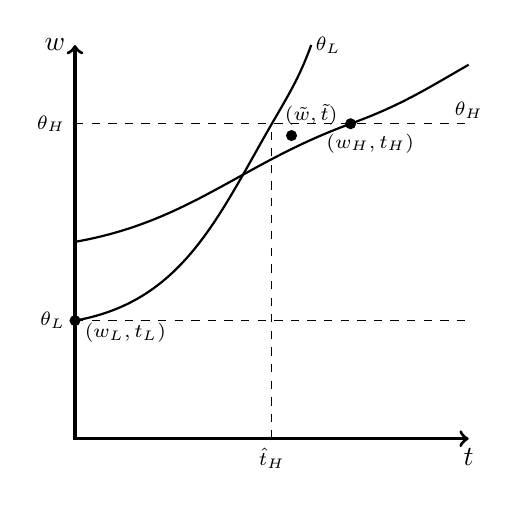
\begin{tikzpicture}[scale=0.5]
			\draw[<->,very thick] (10,0)--(0,0)--(0,10);
			\node[below] at (10,0) {$t$};
			\node[left] at (0,10) {$w$};
			\node[below] at (5,0) {\scriptsize $\hat{t}_H$};
		
		
			\node[left] at (0,3) {\scriptsize $\theta_L$};
			\node[left] at (0,8) {\scriptsize $\theta_H$};
			
			\draw[dashed] (0,3)--(10,3);
			\draw[dashed] (0,8)--(10,8);
			\draw[dashed] (5,0)--(5,8);
			
			\draw[thick] (0,3) to[out=10,in=240] (5,8) to[out=60,in=250] (6,10);
			\draw[thick] (0,5) to[out=10,in=200] (7,8) to[out=20,in=210] (10,9.5);
			\node[below] at (10,8.8) {\scriptsize $\theta_H$};
			\node[left] at (7,10) {\scriptsize $\theta_L$};
			
			
			\fill[black] (5.5,7.7) circle(4pt);
			\fill[black] (7,8) circle(4pt);
			\fill[black] (0,3) circle(4pt);
			\node[above] at (6,7.7) {\scriptsize $(\tilde{w},\tilde{t})$};
			\node[below] at (7.5,8) {\scriptsize $(w_H,t_H)$};
			\node[right] at (0,2.7) {\scriptsize $(w_L,t_L)$};
		\end{tikzpicture}
		\caption{A Pooling Equilibrium}
		\label{fig:screening_separating}
\end{figure}

Our final result is that an equilibrium may not exist in pure strategies. It may instead exist in mixed strategies, but that requires a lot more work. 

Similarly to signaling, the low type is worse off with screening than without. High types, however, are always better off in a separating equilibrium. The issue is that a separating equilibrium may not exist.

\begin{remark}
	To see why, note that since separating equilibria are unique, under certain conditions the agents will want to deviate to a pooling equilibrium, from which they again want to deviate. It's a cycle.
\end{remark}


\subsection{Mechanism Design}

\begin{definition}
	A \blue{mechanism} is a message space $M$ and a mapping $h(\cdot)$ from $M$ to the space of outcomes which can be written as $h(m) = (Q(m),t(m))$, an allocation and a transfer, for all $m \in M$. In a typical case like above, a mechanism will set an allocation and a transfer for the high-skill and low-skill types.
\end{definition}

\begin{remark}
	We can think of the message space as the controls the agent has on the mechanism -- Marco used ``a big table with lots of buttons'' -- each of which matches to an allocation.
\end{remark}

\begin{proposition}
	Any mechanism induces an allocation rule
\end{proposition}

\begin{example}
	Assume here quasilinear preferences $\theta v(Q) - t)$, and let
	\[
	m\opt(\theta) \in \argmax_{m \in M} \theta v(Q(m)) - t(m)
	\]
	Then the induced allocation rule is
	\[
	a(\theta) = Q(m\opt(\theta)),t(m\opt(\theta)))
	\]
\end{example}

\begin{definition}
	A \blue{direct mechanism} is a mechanism in which $M_i = \Theta_i$, meaning that the message space for $i$ is $i$'s type space.
\end{definition}

\begin{question}
	Is there loss of generality in restricting attention to only direct mechanisms? We will see that the answer is no.
\end{question}

\begin{definition}
	A \blue{direct revelation mechanism} is a mapping $g(\cdot)$ from the space of types to the space of outcomes which is written as $g(\theta_i) = (q(\theta_i),T(\theta_i))$. Essentially, the principal commits to offer $q(\theta_i)$ at a price $T(\theta_i)$ if the agent reports type $\theta_i$.
\end{definition}

\begin{definition}
	An agent $\theta$ finds it \blue{incentive compatible} to announce their type truthfully if and only if
	\[
	\theta v(q(\theta)) - T(\theta) \ge \theta v(q(\theta')) - T(\theta') \forall \theta'
	\]
	A direct revelation mechanism is \blue{truthful} if it is incentive compatible for any agent to announce their true type.
\end{definition}

\begin{definition}
	A direct revelation mechanism $g$ is \blue{individually rational} if $\theta v(q(\theta)) - T(\theta) \ge \bar{u}$ where $\bar{u}$ is the reservation utility.
\end{definition}


\begin{theorem}
	\red{(The Revelation Principle)} Any possible allocation rule $a(\theta)$ obtained with a mechanism $\{M,h(\cdot)\}$ can also be implemented with a truthful direct revelation mechanism.
\end{theorem}

\begin{remark}
	This is shockingly powerful and useful! It gives us a way to directly characterize an optimal mechanism. Essentially, we can use a direct revelation mechanism to find what allocation is optimal, and then find a simple mechanism that attains that optimal allocation.
\end{remark}


\begin{proof}
	Assume that we can obtain an allocation $a(\theta)$ with mechanism $\{M,h(\cdot)\}$. This mechanism induces an outcome function
	\[
	g(\theta) = (Q(m\opt(\theta)),T(m\opt(\theta)))
	\]
	We can construct the functions $\hat{Q} = Q \circ m\opt$ and $\hat{T} = T \circ m\opt$. Is this mechanism truthful? Since
	\[
	m\opt(\theta_i) \in \argmax_m \theta_i v(Q(m)) - t(m)
	\]
	it must be the case that
	\[
	\theta_i v\parl \hat{Q}(\theta_i)\parr  - \hat{T}(\theta_i) \ge \theta_i v\parl \hat{Q}(\theta')\parr  - \hat{T}(\theta') \forall \theta'
	\]
	Thus, this direct mechanism is incentive compatible. The proof for individual rationality follows from the same argument.
\end{proof}

\begin{example}
	The optimal direct mechanism with two types. The principal is a monopolist, trying to sell a good to a buyer. The seller's problem can be written as
	\[
	\max_{T_i,q_i} \beta(T_L - cq_L) + (1-\beta) (T_H - cq_H)
	\]
	subject to incentive compatibility and individual rationality. To find a mechanism that maximizes the monopolist's profits, we proceed in steps. The standard approach is to first note that the individual rationality of the low type and incentive compatibility of the high type imply individual rationality of the high type. We can eliminate the individual rationality of the high type constraint. Next, we can consider a relaxed version of this problem where the incentive compatibility constraint of the low type does not bind. If we find a solution of this problem that also satisfies incentive compatibility of the low type, then we will have a solution to the original problem. 
	
	Now we have a simple problem with two constraints, which must both hold with equality. We can substitute, and get an unconstrained optimization problem in just $q_L,q_H$ which is easy to solve with first order conditions. We will find that solution, and then verify that incentive compatibility for the low type is satisfied. If it is, we have a solution to the original problem.
	\end{example}
	
\begin{remark}
	We don't necessarily have concavity here -- be careful with corners!
\end{remark}


\begin{remark}
	The solution here will tell us that high types buy more than low types; high types will buy efficiently and low types will be less than efficient; and the low types will have a surplus of zero, high types receive a positive surplus. This result is very generalizable! It holds with multiple types, and even under continuous types -- in those cases, the highest type will be efficient, and everyone else will be less than efficient.
\end{remark}

































\newpage
\section{Exercises}\label{sec:exercises}

\subsection{Choice (Easley)}

\subsubsection{Easley Homework}

\paragraph{Problems}

\begin{enumerate}
	\item Economists have observed that the default setting in retirement plans seems to affect employees' choices about retirement savings. Using the language from class here is how the observations occur. In each scenario presented to the employee, there are two alternatives: a default percentage of the employee's salary to be deducted and placed in a retirement plan and another percentage of the employee's salary to be deducted and placed in a retirement plan if the employee objects to the default option. So the employee can choose ``not object'' and get the default percentage deducted or ``object'' and get the other percentage deducted. In the following, each scenario is described by a pair consisting of object or not object and the percentage deducted in each case. In scenario I, the alternatives are: ``not object'' and 5 percent; and, ``object'' and 0 percent. In scenario II, the alternatives are: ``object'' and 5 percent; and, ``not object'' and 0 percent.
	\begin{enumerate}
		\item Many people choose the default (the alternative with not objecting) in both scenarios. This is often said to be inconsistent with rational choice. Setup a model of a rational decision maker and show that these choices are inconsistent with rational choice in your model.
		\item In this part of the question, we want to ask if the conclusion in part (a), that the choices are inconsistent with rational choice, necessarily follows from the description of the decision problem as it is presented to the employee. To ask this question you need to describe a set of items, X, that is being considered by the employee and ask if there is a rational preference relation on X that could yield these choices. There are two possible answers. First, there does not exist an X and a rational preference relation on X consistent with these choices. Second, there does exist such an X and a rational preference relation on X consistent with these choices. If you believe that the first is true then prove it; if you believe that the second is true provide an example and show that it works.
		\item In this part of the question we want to ask what happens if additional scenarios are introduced. In scenario III, the alternatives are: do not object and 10 percent; and, object and 5 percent. In scenario IV, the alternatives are: do not object and 10 percent; and object and 20 percent. In scenario V, the alternatives are: do not object and 0 percent; and object and 20 percent. The employee's choices are observed to be: In III---object and 5 percent; In IV---do not object and 10 percent; and, In V---object and 20 percent. Is there a set of alternatives, X, and a rational preference relation on X that could yield all of the choices we observe in the five scenarios? Again, there are two possible answers. First, there does not exist an X and a rational preference relation on X consistent with these choices. Second, there does exist such an X and a rational preference relation on X consistent with these choices. If you believe that the first is true then prove it; if you believe that the second is true provide an example and show that it works.
	\end{enumerate}
	\item A consumer has preference relation $\succsim$ on $\reals_+$ of the form $x \succsim y$ if and only if $x \ge 2y$. Is $\succsim$ a rational preference relation? Explain briefly.
	\item Let $X$ be a finite set of alternatives. Suppose $\succsim$ is a rational preference relation on $X$ and let $C\opt(\cdot,\succsim)$ be the choice function on $X$. Suppose that there are alternatives $x,y \in X$ such that $y \succ x$.
	\begin{enumerate}
		\item Compare $C\opt(B,\succsim)$ and $C\opt(B \setminus \{x\},\succsim)$ for a set of alternatives $B$ containing both $x$ and $y$.
		\item Compare $C\opt(B,\succsim)$ and $C\opt(B \setminus \{x\},\succsim)$ for a set of alternatives $B$ containing $x$ but not $y$.
	\end{enumerate}
	\item Let $X = \{a,b,c\}$ be a set of alternatives and suppose that $(\mathcal{B},C(\cdot))$ is a choice structure for which $\mathcal{B}$ is all non-empty subsets of $X$. Suppose that the choice structure satisfies WARP. You know that $C(\{a,b,c\}) = \{a\}$ but have no other information about $C(\cdot)$. What can you say about $C(A)$ for the remaining $A \in \mathcal{B}$?
	\item Let $X$ be a finite, nonempty set and let $\mathcal{B}$ be all non-empty subsets of $X$, i.e. $\mathcal{B}=\mathcal{P}(X)$. Prove that any choice structure $(\mathcal{B},C(\cdot))$, with $\mathcal{B}=\mathcal{P}(X)$, that satisfies WARP satisfies Sen’s $\beta$.
	\item A consumer has preferences $\succsim$ on $\reals^n_+$ that can be represented by a quasi-concave utility function $u: \reals^n_+ \to \reals_+$. You have been asked to describe the effect of a small tax on good one on the consumer’s demand for good one. To do this you plan to start by solving the consumer’s maximization problem. However, you don’t like solving maximization problems with quasi- concave objective functions and so you plan to use a monotonic transformation $f: \reals_+ \to \reals_+$ of the utility function to replace $u:\reals^n_+ \to \reals_+$ by $v(x) = f(u(x))$ in the maximization problem. Is this valid? Will it give you the same demand as you would have found with the original utility function? Explain.
	\item A consumer purchases goods $x \in \reals^L_+$ with $L \ge 2$ at prices $p$ using wealth $w$. Let $x\opt$ be the consumer's chosen bundle of goods. You know that this consumer's choices satisfy Walras' Law and WARP. Local authorities plan to use a tax on good 1 to discourage the consumption of good 1. Local authorities do not want the consumer to be harmed by this tax so they plan to give the consumer a subsidy that is just enough to make $x\opt$ affordable at the new prices $p = (p_1 + t,p_2,\dots,p_L)$, where $t$ is the tax on good 1. The consumer treats this subsidy as a fixed number $R$ that increases wealth to $w + R$.
	\begin{enumerate}
		\item What happens to the amount of good 1 the consumer purchases? Explain briefly.
		\item What would happen to the amount of good 1 the consumer purchases if there was no subsidy, i.e. $R=0$? Explain briefly.
	\end{enumerate}
	\item A consumer has preference relation $\succsim$ on $[0,1]$ that is represented by the utility function $U(x) = x^2 - x$. Is this consumer's preference relation convex? Explain briefly.
	\item In year 0, a consumer has wealth $w^0 = 1,000$, prices are $(p^0_1,p^0_2) = (10,10)$ and the consumer chooses $(x^0_1,x^0_2) = (50,50)$. In year 1, the consumer has wealth $w^1 = 1,250$ and prices are $(p^1_1,p^1_2) = (15,9)$. For what range of choices of $x_2$ can you conclude that the consumer's choices are inconsistent with the weak axiom? You can assume that the consumer's choices satisfy Walras' Law.
	\item One of your colleagues is interested in comparing the welfare of two people who live in locations where there are different prices for goods and where the two individuals have different wealths. Your colleague believes that these two people have common preferences. Specifically, he assumes that there are two consumers, 1 and 2, with rational and locally non-satiated preferences $\succsim$ over consumption goods in $\reals^L_+$. The prices and wealths for consumers 1 and 2 are $(p^1,w^1)$ and $(p^2,w^2)$ respectively. Each consumer selects a bundle of goods in their budget set that is best according to their preferences. Let these bundles be $x^1$ and $x^2$.
	\begin{itemize}
		\item[(i)] Your colleague asks you to suggest how to interpret data that he might find about prices, wealths and choices. Specifically, he asks for each case below whether you can say that consumer 1 is better off than consumer 2 or consumer 2 is better off than consumer 1
		\begin{itemize}
			\item[a.] $p^1x^2 < w^1$ and $p^2x^1 > w^1$
			\item[b.] $p^1x^2 > w^1$ and $p^2x^1 > w^1$
			\item[c.] $p^1x^2 < w^1$ and $p^2x^1 < w^1$
		\end{itemize}
		For each of these cases, what can you say about who is better off? Explain briefly.
		
		\item[(ii)] Another colleague argues that this entire project (inferring who is better off from these choices) is flawed. This colleague makes the following argument:
		\begin{itemize}
			\item[a.] These two people choose where to live
			\item[b.] Suppose that they each were free to choose either location (there is no cost associated with this choice) and that all attributes of the locations that these people care about are reflected in the consumption goods
			\item[c.] Thus, each person prefers (at least weakly) the location they are in to the other location
			\item[d.] Then as they made different location choices either they have different preferences or at least one of them is indifferent between the locations
			\item[e.] Thus, the assumption of common preferences is flawed, and if they don't have common preferences nothing, other than the fact that each consumer prefers their own consumption bundle to the one chosen by the other consumer, can be inferred from the choices over consumption bundles given locations.
		\end{itemize}
		Briefly evaluate this argument.
	\end{itemize}
\end{enumerate}

\paragraph{Solutions.} (From Gabe's solutions, where he worked with Sara Yoo, except for Problem 7b which are from the given solutions.)

\begin{enumerate}
\item Objecting and rational choice

\begin{itemize}
	\item[(a)] Consider a decision-maker $i$, deciding between alternatives $x^i_5$ and $x^i_0$, which represent the plans that have five percent and zero percent deducted respectively. Define $\succ$ such that $x \succ y$ if $i$ would choose $x$ if given the option. In this model, we have that $x^i_5 \succ x^i_0$ in Scenario I, which from our definition of preference relations implies that $x^i_5 \succsim x^i_0$, and $x^i_0 \not\succsim x^i_5$. However, we have in Scenario II that $x^i_0 \succ x^i_5$, which implies that $x^i_0 \succsim x^i_5$. However, this is a contradiction of the preferences implied earlier, so this decision-maker is not rational.
	
	(Note that this model assumes that the decision-maker cannot be indifferent between the two options. This fits the empirical results, as it appears that the majority of people prefer not objecting. However, this may be a stronger assumption than is warranted.)
	
	\item[(b)] Consider the following set of objects:
	\[
		X = \{ (x_0,o), (x_0,n), (x_5,o), (x_5,n)\}
	\]
	where $o$ denotes objecting and $n$ denotes not objecting. Define the following preference relation over these alternatives, which mirrors the Lexicographic preference relation:
	\[
	x \succeq x' \text{ if } x_2 = n \text{ and } x'_2 = 0, \text{ or } x_2 = x'_2 \text{ and } x_1 \ge x'_1	\]

	where we (arbitrarily) assume that $x_0 > x_5$. This rationalizes the choices made by the decision-maker, where $(x_0,n) \succeq (x_5,o)$ and $(x_5,n) \succeq (x_0,o)$. This preference relation is additionally complete and transitive over $X$ -- indeed, all relationships are strict and ordered, so we have
	\[
	(x_0,n) \succ (x_5,n) \succ (x_0,o) \succ (x_5,o)
	\]	
	
	\item[(c)] These preferences are not rationalizable, as the observed preferences violate transitivity. Taking the new set of objects, and making no assumptions about the form of the revealed preference relation:
	\[
	X = \{ (x_0,o), (x_0,n), (x_5,o), (x_5,n), (x_{10},o), (x_{10},n), (x_{20},o),(x_{20},n)\}
	\]
	our observed preferences are, in scenario order:
	\begin{align*}
		(x_5,n) &\succ (x_0,o) \\
		(x_0,n) &\succ (x_5,o) \\
		(x_{5},o) &\succ (x_{10},n) \\
		(x_{10},n) &\succ (x_{20},o) \\
		(x_{20},o) &\succ (x_0,n)
	\end{align*}
	We can construct the following chain:
	\[
	(x_{5},o) \succ (x_{10},n)\succ (x_{20},o)\succ (x_0,n)\succ (x_5,o)
	\]
	which is a contradiction of transitivity. Since the revealed preferences are not transitive, they are not rationalizable.
\end{itemize}



\item $\succeq$ is not a rational preference relation. Consider $x = 2$, and $y = 3$. $x \not\succeq y$, as $2 \not\ge 6$, but $y \not\succeq x$, as $3 \not\ge 4$. Thus, $\succeq$ is not complete, and so is not rational.

\item We will examine $C^\star(\cdot, \succeq)$.
\begin{itemize}
	\item[(a)] For $B \ni x,y$, $C^\star(B,\succeq) = C^\star(B \setminus \{x\},\succeq)$. To see why, note that the only possible difference between them would require $x \in C^\star(B,\succeq)$. However, from the definition of choice functions, that would require $x \succeq z \forall z \in B$, but $y \in B$ and $y \succ x \Rightarrow x \not\succeq y$. Thus, $x \not\in C^\star(B,\succeq)$, so $C^\star(B,\succeq) = C^\star(B \setminus \{x\},\succeq)$.
	
	\item[(b)] For $B \ni x$ where $y \not\in B$, it may be the case that $C^\star(B,\succeq) \ne C^\star(B \setminus \{x\},\succeq)$. That would require that $x \succeq z \forall z \in B$, which would mean that $x \in C^\star(B,\succeq)$ and $x \not\in C^\star(B\setminus \{x\},\succeq)$. However, if $\exists z \in B \st z \succ x$, it will be the case that $C^\star(B,\succeq) = C^\star(B \setminus \{x\},\succeq)$.
\end{itemize}

\item $X = \{a,b,c\}$, and $(B,C(\cdot))$ is a choice structure where $B = \mathcal{P}(X)$, and $C(\{a,b,c\}) = \{a\}$. We can say that if $a \in A$, $C(A) = \{a\}$. This is because the fact that $a \in C(\{a,b,c\})$, and $b,c \not\in C(\{a,b,c\})$ together imply that $a \succ b$ and $a \succ c$. Thus, for $A \in \{ \{a\},\{a,b\},\{a,c\},\{a,b,c\}\}$, $C(A) = \{a\}$. Also, trivially, $C(\{b\}) = \{b\}$, and $C(\{c\}) = \{c\}$, from the definition of the choice correspondence that $C(X) \subseteq X$ and $C(X) \ne \emptyset \forall X$. We can say nothing about $C(A)$ when $A = \{b,c\}$, as we have no information about whether $b \succeq c$ or $c \succeq b$.

\item (WARP $\Rightarrow$ Sen's $\beta$)

\begin{proof}
	We have that $(\beta, C(\cdot))$ satisfies WARP. Take some $x,y \in A \subset B$, and assume that $x,y \in C(A)$ and $y \in C(B)$. These are the necessary conditions for Sen's $\beta$. By WARP, since $x,y \in A \cap B$, $x \in C(A)$, and $y \in C(B)$, $x \in C(B)$. Thus, since $x \in C(B)$ whenever $x,y \in A \subset B$, $x,y \in C(A)$, and $y \in C(B)$, $(\beta,C(\cdot))$ satisfies Sen's $\beta$.
\end{proof} 

\item From Proposition 2.16, we have that for strictly increasing $f$, if there exists $u$ such that $x \succsim y \Leftrightarrow u(x) \ge u(y)$, then $x \succsim y \Leftrightarrow f(u(x)) \ge f(u(y))$. Thus, this is a valid transformation -- if a bundle $x \in \reals^n_+$ is preferred to $y \in \reals^n_+$, so $x \succsim y$, then $v(x) \ge v(y)$, where $v(x) = f(u(x))$. This transformation will give the same demand as with the original utility function, in terms of bundles of items demanded. To see this, consider that the maximization problem is equivalent to finding an ideal bundle, $x^\star \in \argmax_{x \in \reals^n_+} u(x) \equiv \argmax_{x \in \reals^n_+} v(x)$. Since the set of maximizers of each function are the same, as $u(x) \ge u(y) \Leftrightarrow v(x) \ge v(y)$, the demand will be the same.

\item (Compensating Demand)

\begin{itemize}
	\item[(a)] First, note that by assumption the consumer's demand $x(p,w)$ is homogeneous of degree 0. Thus, the conditions of the law of compensated demand hold, and since the consumer's demand satisfies Walras' law, we have that for their new bundle of goods $x'$
	\[
	(p' - p ) \cdot (x' - x^\star) \le 0 \Longrightarrow t(x_1' - x_1^\star) \le 0
	\]
	Thus, since the tax is strictly positive, $x_1' \le x_1^\star$, so their consumption of good 1 weakly decreases.
	
	\item[(b)] If $R = 0$, we do not have a compensated price change, so we can no longer affirm what will happen with the amount of good 1 the consumer purchases, since it will depend on the type of good it is. For instance, if it is a Giffen good, an increase in its price would generate an increase in its consumed amount
\end{itemize}

\item These preferences are convex. By Proposition 2.32, a utility function representing a preference relation $\succeq$ is quasiconcave if and only if $\succeq$ is convex. Taking the derivatives of $u$, we get that $u'(x) = 1 - 2x$, and $u''(x) = -2$. Since $u''(x) < 0 \forall x \in [0,1]$, $u$ is strictly concave, and by implication quasiconcave, and thus the preferences $\succeq$ that it represents are convex.

\item Note first that since $15 \cdot 50 + 9 \cdot 50 = 1,200 < 1,250$, the bundle $x^0$ is available in the consumer in year 1. Thus, their chosen bundle in year 1 must not have been available to them in year 0. Otherwise, their preferences would violate WARP. In other words, the bundles that violate WARP satisfy:
\[
15 x_1 + 9 x_2 \le 1,250 \qquad \text{ and }\qquad 10x_1 + 10x_2 \le 1,000
\]
Assuming that Walras' Law holds, we have that any amount not spent on $x_2$ is spent on $x_1$, so these equations should hold with equality. Solving them, we get that the minimum number of $x^1_2$ that would not violate WARP is 41.67. If they choose a bundle that contains less $x_2$, it would have been attainable under the year 0 prices, so the choice of $(50,50)$ in year 0 would violate WARP. 

\item (Identifying whether consumers are better off)

\begin{itemize}
	\item[(i)] We consider the three cases:
	\begin{itemize}
		\item[(a)] $p_1x_2 < w_1$ and $p_2 x_1 > w_2$: In this case, we can say that consumer 1 is better off than consumer 2. Specifically, we can see that the bundle $x_2$ is attainable under $(p_1,w_1)$. Since $x_2$ is attainable, it must be that $x_1 \succeq x_2$.
		
		\item[(b)] $p_1x_2 > w_1$ and $p_2 x_1 > w_2$: In this case, we cannot say whether either consumer is better off, as neither of their bundles are attainable to the other. 
		
		\item[(c)] $p_1x_2 < w_1$ and $p_2 x_1 < w_2$: These choices are inconsistent with rationality. To see why, note that $\exists \varepsilon_1 > 0 \st B_{\varepsilon_1}(x_2)$ is entirely contained in the feasible set. By local non-satiation, we have that $\exists x' \in B_{\varepsilon_1} \st x' \succ x_2$. However, since consumer 1 chooses $x_1$, we have that $x_1 \succsim x' \succ x_2 \Rightarrow x_1 \succ x_2$. This implies that consumer 2's choice of $x_2$ violates rationality of their common preferences, as $x_2 \not\succsim x_1$ and $x_1$ is feasible. The same argument applies in reverse, so the choices violate rationality.
	\end{itemize}
	\item[(ii)] This argument makes sense. If we consider the location as another element of their preferences, it would violate WARP for consumer 2 to choose to live in their current location instead of (costlessly) moving to consumer 1's location and being able to attain their better bundle. This argument, and the fact that moving is costless, entirely undermines the assumption that their preferences are identical. 
\end{itemize}
\end{enumerate}

\subsubsection{Outside Questions}

The following are from Stanford ECON 202 Problem Set 1. Questions written by Ilya Segal, answers by Gabe along with Shiqi Yang. Answers not necessarily correct.


\paragraph{Problem 1:} Prove the following statements about preference relations:

\begin{itemize}
    \item[(a)] If $\succsim$ is transitive, then $\succ$ is also transitive.

    \item[(b)] If $\succsim$ is transitive, then $\sim$ is also transitive.

    \item[(c)] If $\succsim$ is complete and transitive, then $\succsim$ is \emph{negatively transitive}: if $x \succsim y$ then for any $z$ either $x \succsim z$ or $z \succsim y$ or both.
\end{itemize}

\medskip

    \begin{itemize}
        \item[(a)] \begin{proof} Take some $x,y,z \in X$ such that $x \succ y$ and $y \succ z$. Since $\succ$ implies $\succsim$, we have that $x \succsim y$ and $y \succsim z$, and since $\succsim$ is transitive, $x \succsim z$. To show that $x \succ z$, it suffices to demonstrate that $z \not\succsim x$. Towards a contradiction, assume that $z \succsim x$. Then we would have that $x \succsim y$, $y \succsim z$, and $z \succsim x$. This holds only when $x \sim y \sim z$. However, we assumed earlier that $x \succ y$, meaning that $x \not\sim y$. This is a contradiction, so $z \not\succsim x$. Since $x \succsim z$, we have that $x \succ z$, and since $x \succ y$ and $y \succ z$ $\Rightarrow$ $x \succ z$, $\succ$ is transitive. \end{proof}

        \item[(b)] \begin{proof} Take some $x,y,z \in X$ such that $x \sim y$ and $y \sim z$. Since $\sim$ implies $\succsim$, we have that $x \succsim y$ and $y \succsim z$, and since $\succsim$ is transitive, $x \succsim z$. To show that $x \sim z$, it suffices to demonstrate that $z \succsim x$. From the definition of $\sim$, we have that $z \succsim y$ and $y \succsim x$. Since $\succsim$ is transitive, $z \succsim x$. Thus, we have that $x \succsim z$ and $z \succsim x$, so $x \sim z$, and since $x \sim y \text{ and } y \sim z \Rightarrow x \sim z$, $\sim$ is transitive. \end{proof}

        \item[(c)] \begin{proof} Take some $z$. Since $\succsim$ is complete, either $y \succsim z$ or $z \succsim y$ or both. If $y \succsim z$, then we have that $x \succsim y$ and $y \succsim z$, which means that $x \succsim z$ because $\succsim$ is transitive. Thus, if $x \succsim y$, either $x \succsim z$ or $z \succsim y$ or both for all $z$. \end{proof}
    \end{itemize}

\paragraph{Problem 2:} (Kreps) Two friends, Larry and Moe, wish to go on vacation together. Individually, they are standard preference maximizers -- their preferences $\succsim_{Larry}$ and $\succsim_{Moe}$ are complete and transitive. They attempt to form a joint preference relation, as follows:
\[
x \succsim^* y \text{ if } x \succsim_{Larry} y \text{ or } x \succsim_{Moe} y
\]
That is, they jointly prefer $x$ to $y$ if \emph{either} Larry or Moe prefer $x$ to $y$. 

Prove that $\succsim^*$ is complete. Show by example that it may not be transitive.

\begin{proof}
    Take some $x,y \in X$. Since $\succsim_{Larry}$ and $\succsim_{Moe}$ are both complete, they will each have preferences over $x$ and $y$. Consider three cases. First, if $x \succsim_{Larry} y$ and $x \succsim_{Moe} y$, then $x \succsim^* y$. Next, if $y \succsim_{Larry} x$ and $y \succsim_{Moe} x$, then $y \succsim^* x$. Finally, if $x \succsim_{Larry} y$ and $y \succsim_{Moe} x$ (or \emph{vice versa}), then $x \succsim^* y$ and $y \succsim^* x$. Thus, $\succsim^*$ is complete, because for arbitrary $x,y \in X$, either $x \succsim^* y$ or $y \succsim^* x$ or both. Note that if either $x \sim_{Larry} y$ or $x \sim_{Moe} y$, then $x \sim^* y$, though that case is captured by the above.
\end{proof}


    Take as an example the case where $z \succsim_{Larry} x \succsim_{Larry} y$ and $y \succsim_{Moe} z \succsim_{Moe} x$. Further, assume that $x \not\succsim_{Larry} z$ and $x \not\succsim_{Moe} z$, so those preferences are strict (\ie, $z \succ_{Larry} x$ and $z \succ_{Moe} x$). We have that $x \succsim_{Larry} y$, so $x \succsim^* y$ and we have that $y \succsim_{Moe} z$, so $y \succsim^* z$. However, we also have that $z \succ_{Larry} x$ and $z \succ_{Moe} x$, meaning that $z \succsim^* x$ and $x \not\succsim^* z$, so $z \succ^* x$. Since $x \succsim^* y$ and $y \succsim^* z \not\Rightarrow x \succsim^* z$, in this case $\succsim^*$ is not transitive.

\paragraph{Problem 3:} A ``problem'' with Proposition 2 in the notes is that it assumes we have the entire choice rule $C$. If we are trying to test the preference-based model of choice, we will typically have less data than all of $C$ in two respects. First, for sets $A \subseteq X$ where $C(A)$ contains more than one element, we are likely to see only one element of $C(A)$. Second, we will typically see $C(A)$ for some, but not all, subsets $A \subseteq X$

\begin{itemize}
    \item[(a)] Show that the first problem is virtually unresolvable. Assume that when we see $x \in A$ being chosen from $A$, this doesn't preclude $y \in A$ being just as good as $x$. Prove that in this case, no data we see will \emph{ever} contradict the preference-based model. (This is a trick question -- if you see the trick, it takes about two lines to answer.)

    \item[(b)] Suppose that we observe $C(A)$ for some, but not all, subsets $A \subseteq X$. That is, we observe a choice rule $C: \mathcal{A} \to \mathcal{B}$, where $\mathcal{A} \subset \mathcal{B}$ is the set of feasible sets the agent is offered. Show that these partial data may satisfy Houthakker's axiom of revealed preference and still be inconsistent with the standard preference-based model.

    \item[(c)] Say that the choice rule $C: \mathcal{A} \to \mathcal{B}$ satisfies the \textbf{General Axiom of Revealed Preference} (GARP) if, for any sequence $A_1,\dots,A_n$ and $x_i \in A_i$ for each $i$, $x_{i+1} \in C(A_i)$ for all $i = 1,\dots,n-1$, and $x_1 \in C(A_n)$ imply that $x_i \in C(A_i)$ for all $i$. (That is, it rules out revealed preference cycles except for revealed indifference.) Show that if the set $X$ of choices is finite, a nonempty-valued choice function $C: \mathcal{A} \to \mathcal{B}$ is rationalizable by a complete transitive preference if and only if it satisfies GARP. (Note: the ``if'' part is hard.)
\end{itemize}

\medskip

\begin{itemize}
    \item[(a)] \begin{proof} Note first that proving that a set of preferences violates transitivity requires proving that at least one preference is strict, in order to rule out transitive indifference. Under these conditions, if $x \succ y$, then $C(\{x,y\}) = x$, but it is impossible to rule out that $y \succsim x$. Thus, no data will ever contradict the preference-based model. \end{proof}

    \item[(b)] Take some $x,y,z \in X$ such that $x \succ y$, $y \succ z$, and $z \succ x$. Also assume that $\mathcal{A} = \{x,y\}$, so we only observe $C(A) = x$ and no other choices. HARP is vacuously true, but the preferences as stated clearly violate transitivity.  

    \item[(c)] 
    \begin{proof}
        $(\Longrightarrow)$ We have that a nonempty-valued choice function $C : \mathcal{A} \to \mathcal{B}$ is rationalizable by a complete transitive preference. Towards a contradiction, assume that GARP is not satisfied, so there exists a sequence $A_1,\dots,A_n$, $x_i \in A_i$ for each $i$, $x_{i+1} \in C(A_i)$ for all $i = 1,\dots,n-1$, and $x_1 \in C(A_n)$ but there is some $x_i \not\in C(A_i)$. Since $x_{i+1} \in C(A_i)$, $x_{i+1} \succ x_i$. However, note that $x_i \in C(A_{i-1})$, so $x_i \succsim x_{i-1}$, and $x_{i-1} \in C(A_{i-2})$, so $x_{i-1} \succsim x_{i-2}$, and so on. Since $x_1 \in C(A_n)$, $x_1 \succsim x_n$. Thus, we have
        \[
        x_i \succsim x_{i-1} \succsim \cdots \succsim x_1 \succsim x_n \succsim x_{n-1} \succsim \cdots \succsim x_{i+1}
        \]
        Since transitivity extends to all $n$-cycles, and $x_{i+1} \succ x_i$ (which implies that $x_i \not\succsim x_{i+1}$, this violates transitivity. This contradicts the earlier assumption that $C$ is rationalizable by a complete transitive preference, so GARP must be satisfied.

        \medskip

        $(\Longleftarrow)$ We have that $C: \mathcal{A} \to \mathcal{B}$ satisfies GARP, so for any sequence $A_1,\dots,A_n$ and $x_i \in A_i$ for each $i$, $x_{i+1} \in C(A_i)$ for all $i = 1,\dots,n-1$, and $x_1 \in C(A_n)$ imply that $x_i \in C(A_i)$ for all $i$. We will demonstrate that it is rationalizable by a complete transitive preference. 

        Define $x \succsim^r y$ if $x \in C(A)$ and $y \in A$. Say that a sequence $x_1,\dots,x_n$ is a chain if $x_{i+1} \succsim^r x_i$ for all $i$. Say that a cycle is a chain where $x_1 = x_n$. Note that a cycle can be contained in a chain. Also note that $\succsim^r$ is not complete (if the only $A$ where $x,y \in A$ is such that $x,y \not\in C(A)$, we can say nothing about their relationship) nor necessarily transitive (we cannot say whether $x \succsim^r z$ if there is no $A$ such that $z \in A$ and $x \in C(A)$, no matter if $x \succsim^r y$ and $y \succsim^r z$). 

        Define $x \succsim^t y$ if either $x \succsim^r y$ or there exists a chain containing both $x$ and $y$ where $x \succsim^r \cdots \succsim^r y$. Note that if $x$ and $y$ are in a cycle, then $x \sim^t y$.
        
        Define a cycle $C$ as a complete cycle if there exists no $y \not\in C$ where $x \succsim^t y$ or $y \succsim^t x$ for any $x \in C$. Note that all elements which are not comparable to any other elements are singleton complete cycles.

        Begin with a sequence $A = A_1,\dots,A_n$ where $x_i \in A_i$ and $x_{i+1} \in C(A_i)$ for each $i$, so it is a chain $C$. We say that this chain can be extended downward if $\exists$ $A_0$ such that $x_1 \in C(A_0)$ and $x_0 \in A_0$ for some $x_0 \ne x_1$. We say that this chain can be extended upward if $\exists$ $A_{n+1}$ where $x_{n+1} \in C(A_n)$ for some $x_{n+1} \in A_{n+1}$. All chains which cannot be extended we call maximal chains. We call a chain $C$ a complete chain if that chain is maximal and if $x_i \in C$ is also in a cycle, all other elements $x_{i+1},\dots$ of the cycle are also in the chain.

        Note that all elements of $X$ are also elements of either a complete chain or a complete cycle. Next, we will demonstrate that the elements can be ordered by a utility function, so they can be compared. Define a length function $l$ such that for a complete chain $C = x_1,\dots,x_n$, $l(c) = n - 1 - n_c + N_c$, where $n$ is the number of elements in the chain, $n_c$ is the number of elements of the chain which are also in a cycle, and $N_c$ is the number of cycles in the chain. Note that $l(C) = 0$ whenever $C$ is a complete cycle. This definition is only possible because GARP ensures that there are no revealed preference cycles except for revealed indifference -- if there existed $x \succ y \succ z \succ x$, there would exist non-cyclical chains of infinite length. Since we assumed GARP held, $l$ has finite range.

        Construct a utility function as follows. All elements which are part of a complete chain have minimal utility (they are assigned utility of $-\infty$). Define the set of complete maximal chains $\mathcal{C} = \{C_1,\dots,C_n\}$. This will be a finite set because $X$ is finite, so the length function $l: \mathcal{C} \to \integers_+$ attains a maximum over it. Take all the chains for which $l$ is maximized, and assign their maximal elements utility of 0 (an element $x$ of a complete chain $C$ is maximal if $x \succsim^t y$ for all $y \in C$). Then remove all of those elements from the chains and find the new chains over which $l$ attains a maximum. Assign their maximal elements utility of $-1$, and continue this process until all elements of all complete chains are assigned. (The process will end because $X$ is finite.)

        We have now assigned a utility to every element of $X$, and the process guarantees we have not assigned two utilities to the same element. Let $\succsim^\star$ be the preference relation generated by this utility relation, so $x \succsim^\star y$ if the utility assigned to $x$ is greater than or equal to the utility assigned to $y$. It remains to show that $\succsim^\star$ is complete and transitive, and that it generates the choice rule $C$ we began with.

        First, as stated above each element is assigned a utility, so the completeness of $\ge$ on $\reals$ ensures that $\succsim^\star$ is complete. The same argument applies to transitivity, where since $\ge$ is transitive on $\reals$, $x \succsim^\star y$ and $y \succsim^\star z$ imply that $u(x) \ge u(y)$ and $u(y) \ge u(z)$, so $u(x) \ge u(z)$ and $x \succsim^\star z$.

        Finally, we will show that $C_{\succsim^\star}$, the choice rule generated by $\succsim^\star$, is equivalent to $C$, our initial choice rule. It suffices to show that $C_{\succsim^\star}(A) \subseteq C(A)$ and that $C_{\succsim^\star}(A) \supseteq C(A)$.

        $(\subseteq)$ Suppose that $x \in C_{\succsim^\star}(A)$. Then for each $y \in A$, $u(x) \ge u(y)$. Towards a contradiction, assume that $x \not\in C(A)$. Then there must exist $y \in A$ such that $y \succsim^r x$. By construction, $u(y) \ge u(x)$ because there exists at least one chain where $y \succsim^r x$. This implies that $y \succsim^\star x$, meaning that $u(y) \ge u(x)$. However, this implies that $u(y) = u(x)$, which can only be the case when $x$ and $y$ are in a cycle, so by GARP, $x \in C(A)$. This is a contradiction of the assumption that $x \not\in C(A)$, so $x$ must be in $C(A)$.

        $(\supseteq)$ Suppose that $x \in C(A)$, and $y \in A$. Then it must be true that $x \succsim^r y$, and by construction $u(x) \ge u(y)$ because there exists at least one chain where $x \succsim^r y$. Since $u(x) \ge u(y)$, $x \succsim^\star y$ and $x \in C_{\succsim^\star}(A)$. 

        
    \end{proof}

\end{itemize}
\paragraph{Problem 4:} Is the lexicographic preference relation (a) complete, (b) transitive, (c) strictly monotone, (d) convex, (e) continuous?

\medskip

\begin{itemize}
    \item[(a)] The lexicographic preference relation is complete.

    \begin{proof}
        Consider $x,y \in X = [0,1]^2$, where $x = (x_1,x_2)$ and $y = (y_1,y_2)$. Since the real numbers are an ordered field, we know that for $a,b \in \reals$, either $a > b$, $b > a$, or $a = b$. Thus, either $x_1 > y_1$, in which case $x \succ y$, $y_1 > x_1$, in which case $y \succ x$, or $x_1 = y_1$. In this final case, either $x_2 > y_2$, in which case $x \succ y$, $y_2 > x_2$, in which case $y \succ x$, or $x_2 = y_2$, in which case $y \sim x$. Thus, the lexicographic preference relation is complete, because $\succ$ and $\sim$ each individually imply $\succsim$.
    \end{proof}

    \item[(b)] The lexicographic preference relation is transitive.

    \begin{proof}
        Consider $x,y,z \in X = [0,1]^2$ such that $x \succsim y$ and $y \succsim z$. Consider first the case where those relations are both indifferent, so $x \sim y$ and $y \sim z$. From the definition of the lexicographic preference relation, that means that $x_1 = y_1$ and $x_2 = y_2$, as well as $y_1 = z_1$ and $y_2 = z_2$. Since equality is transitive over $\reals$, that means that $x_1 = z_1$ and $x_2 = z_2$, so $x \sim z \Rightarrow x \succsim z$. Next, consider the case where one of those relations is strict. Without loss of generality, assume that $x \succ y$. This implies that either $x_1 > y_1$ or $x_1 = y_1$ and $x_2 > y_2$. We also have that $y_1 \ge z_1$, so if $x_1 > y_1$, $x_1 > z_1$ and $x \succ z$. If $x_1 = y_1$, then either $y_1 > z_1$ (which implies that $x_1 > z_1 \Rightarrow x \succ z$) or $y_1 = z_1$ and $y_2 \ge z_2$. Since $x_2 > y_2$, $x_2 > z_2$ by transitivity of the reals and $x \succ z$. Thus, since $\succ$ and $\sim$ each individually imply $\succsim$, whenever $x \succsim y$ and $y \succsim z$, $x \succsim z$ and lexicographic preference relation is transitive.
    \end{proof}

    \item[(c)] The lexicographic preference relation is strictly monotone.

    \begin{proof}
        Take $x,y \in X$ such that $x \gg y$. This means that $x_1 > y_1$, so $x \succ y$.
    \end{proof}

    \item[(d)] The lexicographic preference relation is convex.

    \begin{proof}
        Take $x,x',y \in X$ such that $x \succsim y$ and $x' \succsim y$. This means that $x_1 \ge y_1$ and $x'_1 \ge y_1$. Thus, $tx_1 + (1-t)x'_1 \ge y_1$ for all $t \in (0,1)$, because the affine combination of two real numbers will be greater than the smaller of the two (unless they are equal), which is itself at least as large as $y_1$. If the combination is strictly greater, than $tx + (1-t)x' \succ y$. If it is equal, then both $x_1$ and $x_1'$ must be equal to $y_1$. Since $x \succsim y$ and $x' \succsim y$, that means that $x_2 \ge y_2$ and $x'_2 \ge y_2$, and by the same logic $tx_2 + (1-t)x'_2 \ge y_2$ for all $t \in (0,1)$. If that is a strict difference, then $tx + (1-t)x' \succ y$. If they are equal, then both $x_2$ and $x'_2$ must be equal to $y_2$, and $tx + (1-t)x' \sim y$. Since $\succ$ and $\sim$ each individually imply $\succsim$, $x \succsim y$ and $x' \succsim y$ implies that  $tx + (1-t)x' \succsim y$ for all $t \in (0,1)$, and the lexicographic preference relation is convex.
    \end{proof}

    \item[(e)] The lexicographic preference relation is not continuous.

    \smallskip
    
    Take as a counterexample the sequences $x^n = (0.5 + \frac{1}{n},0)$ and $y^n = (0.5 - \frac{1}{n},1)$, for $n = 2,\dots$. By inspection, $x^n \to x = (0.5,0)$ and $y^n \to y = (0.5,1)$. The first term of each element of $x^n$, $x^n_1$, is strictly greater than $0.5$, and the first term of each element of $y^n$, $y^n_1$, is strictly less than $0.5$, since $\frac{1}{n} > 0$. This means that $x^n_1 > y^n_1$ for all $n$, so $x^n \succ y^n$ for all $n$. However, $x_1 = y_1 = 0.5$, and since $y_2 = 1 > x_2 = 0$, $y \succ x$. This contradicts the definition of continuity, so the lexicographic preference relation is not continuous.

    \bigskip

    \textbf{Shorter Answer:} Yes, yes, yes, yes, no.

    
\end{itemize}
\paragraph{Problem 5:} Prove that if $u : X \to \reals$ is a continuous utility function representing $\succsim$, then $\succsim$ is continuous.

\medskip

\begin{proof}
    Recall the definition of a continuous real-valued function: such a function is continuous if for any sequence $x^n$ where $x^n \to c$, $f(x^n) \to f(c)$. Also recall that if $u$ represents $\succsim$, then $x \succsim y \Longleftrightarrow u(x) \ge u(y)$. Take sequences $x^n \to x$ and $y^n \to y$, where $x^n \succsim y^n$ for all $n$. We know from above that $u(x^n) \ge u(y^n)$ for all $n$, and $u(x^n) \to u(x)$ as well as $u(y^n) \to u(y)$. We will demonstrate that $u(x) \ge u(y)$, which suffices to show that $x \succsim y$ and that $\succsim$ is continuous.

    Towards a contradiction, assume that $u(y) > u(x)$. For some $\varepsilon > 0$, $u(y) = u(x) + \varepsilon$. Take $\delta = \varepsilon / 3$. From the definition of the limit of a sequence, there exists $N_x$ such that $\forall \; n > N_x$, $u(x^n) \in (u(x) - \delta,u(x) + \delta)$, and there exists $N_y$ such that $\forall \; n > N_y$, $u(y^n) \in (u(y) - \delta,u(y) + \delta)$. However, since $u(y) = u(x) + \varepsilon$, $u(y) - \delta > u(y) - \varepsilon / 2 = u(x) + \varepsilon / 2 > u(x) + \delta$. This means that the two sets are disjoint, where the $\delta$-ball around $u(y)$ lies above the $\delta$-ball around $u(x)$. This implies that, for all $n > \max\{N_x,N_y\}$, $u(y^n) > u(x^n)$. This is a contradiction, since that means that $y^n \succ x^n$ for some $n$, contradicting the assumption that $x^n \succsim y^n$ for all $n$. Thus, $u(x) \ge u(y)$, meaning that $x \succsim y$, and $\succsim$ is continuous.
\end{proof}

\paragraph{Problem 6:} A preference relation $\succsim$ on $\reals^n_+$ is called \emph{homothetic} if for all $x,y \in \reals^n_+$ and all $\lambda > 0$, $x \succsim y$ if and only if $\lambda x \succsim \lambda y$. Show that a continuous strictly monotone preference relation on $\reals^n_+$ is homothetic if and only if it can be represented by a utility function $u : \reals^n_+ \to \reals_+$ with the property $u(\lambda x) = \lambda u(x)$ for all $x \in \reals^n_+$ and all $\lambda > 0$. (This property is known as \emph{homogeneity of degree one}.)

\medskip

\begin{proof} 
    ($\Longleftarrow$) We have that a continuous strictly monotone preference relation can be represented by a utility function $u : \reals^n_+ \to \reals_+$ with the property $u(\lambda x) = \lambda u(x)$ for all $x \in \reals^n_+$ and all $\lambda > 0$. That means that $x \succsim y \Longleftrightarrow u(x) \ge u(y)$. Take some $x,y \in \reals^n_+$ such that $x \succsim y$, which implies that $u(x) \ge u(y)$. Fix some $\lambda > 0$. Multiplying by $\lambda$ and using homogeneity of degree one, we get that $\lambda u(x) \ge \lambda u(y) \Longrightarrow u(\lambda x) \ge u(\lambda y) \Longrightarrow \lambda x \succsim \lambda y$, so $x \succsim y \Longrightarrow \lambda x \succsim \lambda y$. Going the other direction, take some $x,y \in \reals^n_+$ such that $\lambda x \succsim \lambda y$, which implies that $u(\lambda x) \ge u(\lambda y)$. Using homogeneity, we have that $\lambda u(x) \ge \lambda u(y)$, and dividing out the $\lambda$, we have $u(x) \ge u(y)$, which implies that $x \succsim y$. Thus, we have that $x \succsim y \Longleftrightarrow \lambda x \succsim \lambda y$, and $\succsim$ is homothetic.
    
    \medskip

    ($\Longrightarrow$) Take a homothetic preference relation $\succsim$ on $\reals^n_+$, so for all $x,y \in \reals^n_+$ and all $\lambda > 0$, $x \succsim y \Longleftrightarrow \lambda x \succsim \lambda y$. An extension of this property is that $x \sim y \Longleftrightarrow \lambda x \sim \lambda y$. (This holds because $y \succsim x \Longleftrightarrow \lambda y \succsim \lambda x$.) Note that we are assuming that $\succsim$ is complete and transitive, as Ilya said in office hours.\footnote{This direction of the proof does not work if we cannot assume transitivity, because any utility representation would violate the inherent transitivity of $\ge$ over the reals, and it does not work without completeness because there would have to be undefined elements in the domain of $u$.} As such, we assume that $\succsim$ is transitive. Define $e = (1,1,\dots,1)$. From the proof of Proposition 4, for all $x$ there exists a certain $\alpha_x \in \reals_+$ such that $\alpha_x e \sim x$. Define $u(y) = \{ \alpha : \alpha e \sim y\}$. From the proof of Proposition 4, this set will be a singleton for all $y \in \reals^n_+$, so $u$ is well-defined, and $u(x) = \alpha_x$. Since $\succsim$ is homothetic, $\lambda \alpha_x e \sim \lambda x$. This means that $u(\lambda x) = \lambda \alpha_x = \lambda u(x)$, so $u$ is homogeneous of degree one.

\end{proof}

\paragraph{Problem 7:} Suppose the agent lives for $T$ periods, and he chooses a consumption stream $(x_1,\dots,x_T) \in X_1 \times \dots \times X_T$. Suppose that the agent's preferences over consumption streams do not change over time (this is known as ``time-consistency''), and that they are represented by a utility function $u : X_1 \times \dots \times X_T \to \reals$. Derive a necessary and sufficient condition on $u$ for the agent's preferences over future consumption $(x_t,\dots,x_T) \in X_t \times \dots \times X_T$ at any time $t = 2,\dots,T$ to be independent of past consumption $(x_1,\dots,x_{t-1}) \in X_1 \times \dots \times X_{t-1}$. Give examples of utility functions that do and do not satisfy this condition.

\medskip

\textbf{Solution:} To define a necessary and sufficient condition such that preferences over future consumption are independent of past consumption at any time, we will apply Proposition 6 for all $t = 2,\dots,T-1$. Assume that preferences over future consumption at $t = 2$ are independent of past consumption, so $(x_2,\dots,x_T)$ are independent of $x_1$. By Proposition 6, there must exist functions $v_1 : X_2 \times \cdots \times X_T \to \reals$ and $U_1 : \reals \times X_1 \to \reals$ such that $U_1$ is increasing in its first argument and $u(x_1,\dots,x_T) = U_1(v_1(x_2,\dots,x_T),x_1)$. 

Fix some $x_1$. We have that $(x_1,x_2,\dots,x_T) \succsim (x_1,x'_2,\dots,x'_T)$ if and only if $u(x_1,x_2,\dots,x_T) \ge u(x_1,x'_2,\dots,x'_T)$, which is equivalent to the statement $U_1(v_1(x_2,\dots,x_T),x_1) \ge U_1(v_1(x'_2,\dots,x'_T),x_1)$. Since $U_1$ is increasing in its first argument, $(x_1,x_2,\dots,x_T) \succsim (x_1,x'_2,\dots,x'_T)$ if and only if $v_1(x_2,\dots,x_T) \ge v_1(x'_2,\dots,x'_T)$, so $v_1$ represents preferences over $(x_2,\dots,x_T)$ which are independent of $x_1$.

Now consider preferences over $(x_3,\dots,x_T)$. Since those preferences are independent of $x_2$, from the logic above there exist functions $v_2 : X_3 \times \cdots \times X_T \to \reals$ and $U_2 : \reals \times X_2 \to \reals$ such that $U_2$ is increasing in its first argument and $u(x_1,\dots,x_T) = U_1(U_2(v_2(x_3,\dots,x_T),x_2)x_1)$.

We will continue this argument for all $t = 3,\dots,T-1$. We arrive at the following condition: there must exist functions $U_t : \reals^2 \to \reals$ for each $t = 2,\dots,T-1$ and $v_{T-1} : X_T \to \reals$ such that
\[
u(x_1,\dots,x_T) = U_1(U_2(U_3(\dots U_{T-1}(v_{T-1}(x_T),x_{T-1}) \dots,x_3)x_2)x_1)
\]
for all $x \in \reals^n_+$, where each $U_t$ is increasing in its first argument.

By Proposition 6, this condition is necessary to show that preferences on $(x_t,\dots,x_T)$ do not depend on $(x_1,\dots,x_{t-1})$ at any time $t = 2,\dots,T$. To demonstrate that it is sufficient, assume that there exist functions $U_t : \reals^2 \to \reals$ for all $t = 2,\dots,T-1$ and $v_{T-1} : \reals \to \reals$ such that each $U_t$ is increasing in its first argument and
\[
u(x_1,\dots,x_T) = U_1(U_2(U_3(\dots U_{T-1}(v_{T-1}(x_T),x_{T-1}) \dots,x_3)x_2)x_1)
\]
For each period $1 < t < T$, define $\Tilde{v}_t : \reals^{T-t+1} \to \reals$, where
\[
\Tilde{v}_t(x_t,\dots,x_T) = U_{t}(U_{t+1}(U_{t+2}(\dots U_{T-1}(v_{T-1}(x_T),x_{T-1}) \dots,x_{t+2})x_{t+1})x_t)
\]
Also define $\Tilde{U}_t : \reals^t \to \reals$, where
\[
\Tilde{U}_t(v_t(x_t,\dots,x_T), x_1,\dots,x_{t-1}) = U_1(U_2(U_3(\dots U_{T-1}(\Tilde{v}_{t}(x_t,\dots,x_T),x_{t}) \dots,x_3)x_2)x_1)
\]
From above, we have that $u(x_1,\dots,x_T) = \Tilde{U}_t(v_t(x_t,\dots,x_T), x_1,\dots,x_{t-1})$, and since the implied first argument of $\Tilde{U}_t$ is $U_{t+1}$ which is increasing in its first argument means that $\Tilde{U}_t$ is increasing in its first argument, by Proposition 6, preferences over future consumption do not depend on past consumption.

Thus, we have derived a necessary and sufficient condition that preferences over future consumption do not depend on past consumption at any time $t = 2,\dots,T$.

\medskip

As an example of a utility function which does satisfy this condition, consider a linear utility function that is a sum over all consumption, so $u(x_1,\dots,x_T) = \sum_{i=1}^T x_i$. For a utility function which does not satisfy this condition, consider a utility function which depends on the difference between consumption in period $i$ and period $i-1$, so $u(x_1,\dots,x_T) = \sum_{i=1}^T (x_i - x_{i-1})$, fixing $x_0 = 0$. 

\newpage
\subsection{Consumer (Kircher)}

\subsubsection{Kircher Homework}

\paragraph{Problems}

\begin{enumerate}
	\item Study Berge’s Maximum Theorem, and make a short video (no longer than 2 minutes) in which you explain its basic insight and intuition in your own words using a single graph that you share on screen
	\item Imagine a worker who chooses how much to work ($t$) and how much to consume ($x$), where each of them is a non-negative scalar. The worker earns a wage normalized to 1 per hour worked, but only has $w$ hours available. The consumers utility function of work and consumption is given by $u(x,t) = \parl x^{1/2} + (w-t)\parr^2$. Assume that the hours budget $w$ and the price of the consumption good $p$ are the only free variables in the model (i.e., no changes in the wage rate).
	\begin{enumerate}
		\item Write the workers problem in a more conventional way by writing his utility function in terms of consumption $x$ and leisure $l$, given a budget constraint.
		\item Find the worker’s Walrasian demand functions for goods $x$ and $l$.
		\item Find the worker’s indirect utility function using the utility function given in the statement of this problem.
		\item Suppose that time endowment $w$ and price $p$ are such that the worker chooses some strictly positive level of leisure. Find the worker’s Hicksian demand function for good $x$ for price and utility levels consistent with strictly positive purchases of leisure.
	\end{enumerate}
	\item Consider a consumer with an expenditure function $e(p,u)$ that is multiplicatively separable in the sense that $e(p,u)=g(u)r(p)$ for some strictly increasing function $g(u)$ and strictly increasing function $r(p)$.
	\begin{enumerate}
		\item Find this consumer's Walrasian demand function.
		\item Exploit Walras' Law to show that $r(p) = \sum_{i=1}^L p_i \frac{\partial r(p)}{\partial p_i}$. Do you need to make any assumptions on $g(u)$ to arrive at this equality?
		\item Now suppose there is a finite number $M$ of consumers in the economy that all share this expenditure function but that might not have the same budget. Does the distribution of budgets matter for aggregate demand? (If not, it means that you created a representative agent economy)
	\end{enumerate}
	\item Consider a consumer that makes choices how much to buy of two different products given a budget constraint. You happen to know that the expenditure function of the consumer it is of form $e(p,U) = Up^\alpha_1 p_2^\beta$
	\begin{enumerate}
		\item What restrictions (if any) on the parameters $\alpha$ and $\beta$ are required to ensure that $e(.)$ constitutes a valid expenditure function. Assume that the restriction(s) are/is satisfied.
		\item Find the indirect utility function, the Hicksian demand functions, and the uncompensated demands. Carefully list the correct arguments for each function.
		\item Use an alternative approach — i.e. different to what you did in b) — to calculate the uncompensated demand functions.
		\item Assume the consumer has $\alpha = \beta = 1/2$, and a budget of 512. Assume environmental legislation increases prices from $p_1 = p_2 = 1$ to $p_1 = p_2 = 16$. One way to think about how to assess the loss of welfare for this consumer due to the price increase is to ask how much money would one have to give this consumer to be equally well off. There are two ways of doing this.
		\begin{enumerate}
			\item What is the compensating variation for this consumer? What is the equivalent variation for this consumer?
			\item If compensating variation and equivalent variation differ, explain why one is higher than the other in an intuitive way. Which one would you think is more reasonable if one intended to pay this consumer for his consent to agree to the price increase?
		\end{enumerate}
	\end{enumerate}
	\item Evaluate the following (explain your answer):
	\begin{enumerate}
		\item Consider utility function $u(x) = 2\ln(x_1) + 2\ln(x_2)$ and associated expenditure function $e(u,p_1,p_2)$. Now consider the utility function $u\opt(x) = x_1x_2$ with associated expenditure function $e\opt$. Claim to evaluate: $e(u,p_1,p_2) = e\opt(u\opt,p_1,p_2)$ if $u\opt = \exp(u / 2)$.
		\item Consider a consumer with continuous and locally non-satiated preferences and income $w$ who consumes strictly positive amounts of all goods at a given price vector $p\gg 0$. Now the price of good $i$ increases from $p_i$ to $p'_i$, while all other prices stay the same. Assume his income increases by $(p_i' - p_i)x_i(p,w)$. Claim to evaluate: this consumer always purchases less of good $i$ under the new prices compared to the old prices, and obtains a higher utility under the new prices.
		\item A consumer who will live for $T \ge 2$ periods has utility function $\sum \beta^t u(c_t)$ for consumption path $c = (c_1,\dots,c_T)$. Assume that $0 < \beta < 1$, $u'(c) > 0$ and $u''(c) < 0$ for all $c \ge 0$, and $\lim_{c\to0}u'(c) = \infty$. Consumption in each period must be non-negative and total consumption can be no more than wealth $w > 0$, i.e. $\sum c_t \le w$. Claim to evaluate: Optimal consumption $c_t\opt$ can increase under some utility functions.
	\end{enumerate}
	\item Find an (interesting?) research paper in industrial organization, labor economics, health economics, or some other area of economics that relies on the insights from consumer theory that we discussed in class. Which insights in particular are they using?
\end{enumerate}

\paragraph{Solutions.} (Gabe's solutions, completed with Sara Yoo and Omar Andujar. Corrected original answers to 2c and 5b after TA feedback)
\begin{enumerate}
	\item I'm not posting a video here LMAO
	\item We have a consumer whose utility function is $u(x,t) = \parl x^{\frac{1}{2}} + (w - t)\parr^2$
	\begin{enumerate}
		\item We have that the consumer is solving
		\[
		\max_{x,l \in \reals_{+}} u(x,l) = \parl x^{\frac{1}{2}} + l\parr^2
		\]
		subject to
		\[
		px \le w - l \equiv px + l \le w
		\]
		\ie, they are maximizing consumption and leisure subject to consumption not exceeding their wage for the total hours worked.
		\item Our Lagrangian is
		\[
		\mathcal{L} = \parl x^{\frac{1}{2}} + l\parr^2 + \lambda(w - l - px)
		\]
		For the first order conditions, we get
		\[
		\frac{\partial \mathcal{L}}{\partial x} = \frac{x^{1/2} + l}{x^{1/2}} - p\lambda = 0 \Longrightarrow \lambda = \frac{x^{1/2} + l}{p\cdot x^{1/2}}
		\]
		\[
		\frac{\partial \mathcal{L}}{\partial l} = 2x^{1/2} + 2l - \lambda = 0 \Longrightarrow \lambda = 2x^{1/2} + 2l
		\]
		\[
		\frac{\partial \mathcal{L}}{\partial \lambda} = w - l - px = 0 \Longrightarrow  px+ l = w
		\]
		Setting them equal and solving, we get that
		\[
		\frac{x^{1/2} + l}{p\cdot x^{1/2}} = 2x^{1/2} + 2l \Longrightarrow 2px^{1/2}(x^{1/2} + l) = x^{1/2} + l
		\]
		so we get that the Walrasian demand for $x$ is
		\[
		x^\star = \frac{1}{4p^2}
		\]
		and inputting into the budget constraint, we get
		\[
		\frac{p}{4p^2} + l = w \Longrightarrow l^\star = w - \frac{1}{4p}
		\]
		Note that this might create a corner solution -- if $w < \frac{1}{4p}$, then the consumer always work. Formally, our Walrasian demand functions are
		\[
		x^\star(p,w) = \begin{cases} \frac{1}{4p^2} & w \ge \frac{1}{4p} \\ w & \text{otherwise} \end{cases}
		\]
		and
		\[
		l^\star(p,w) = \begin{cases} w - \frac{1}{4p} & w \ge \frac{1}{4p} \\ 0 & \text{otherwise} \end{cases}
		\]
		\item Going back to the originally stated utility function, the indirect utility function is defined by
		\[
		V(p,w) \coloneqq \max_{x,t \in \reals_+} \parl x^{\frac{1}{2}} + (w - t)\parr^2
		\]
		subject to
		\[
		px \le t
		\]
		We first solve for the Walrasian demand functions. Our Lagrangian is
		\[
		\mathcal{L} = \parl x^{\frac{1}{2}} + (w - t)\parr^2 + \lambda (t - px)
		\]
		and our first order conditions are
		\[
		\frac{\partial \mathcal{L}}{\partial x} = \frac{x^{1/2} + w - t}{x^{1/2}} - p\lambda = 0 \Longrightarrow \lambda = \frac{x^{1/2} + w - t}{px^{1/2}}
		\]
		\[
		\frac{\partial \mathcal{L}}{\partial t} = -2\parl x^{1/2} + w - t\parr + \lambda = 0 \Longrightarrow \lambda = 2\parl x^{1/2} + w - t\parr
		\]
		\[
		\frac{\partial \mathcal{L}}{\partial \lambda} = t - px = 0 \Longrightarrow t = px
		\]
		Which implies that
		\[
		2\parl x^{1/2} + w - t\parr = \frac{x^{1/2} + w - t}{px^{1/2}} \Longrightarrow  x^\star = \frac{1}{4p^2}
		\]
		and
		\[
		t^\star = px^\star = \frac{1}{4p}
		\]
		which is the same as above, a confirmation that this formulation also works. As above, we have admitted a corner, where the worker will not take any time off if $\frac{1}{4p} > w$. Formally, our Walrasian Demand is
		\[
		x^\star(p,w) = \begin{cases} \frac{1}{4p^2} & w \ge \frac{1}{4p} \\ w & \text{otherwise} \end{cases}
		\]
		and
		\[
		t^\star(p,w) = \begin{cases} \frac{1}{4p} & w \ge \frac{1}{4p} \\ w & \text{otherwise} \end{cases}
		\]
		
		From the definition of the indirect value function, we have that in the interesting case,
		\[
		V(p,w) = u(x^\star,t^\star) = \parl \parl \frac{1}{4p^2}\parr^{\frac{1}{2}} + \parl w - \frac{1}{4p}\parr \parr^2 = \parl \frac{1}{2p} + w - \frac{1}{4p} \parr^2 = \parl \frac{1}{4p} + w\parr^2
		\]
		so our final attained value function is
		\[
		V(p,w) = \begin{cases} \parl \frac{1}{4p} + w\parr^2 & w \ge \frac{1}{4p} \\ w & \text{otherwise}\end{cases} 
		\]
		\item For leisure to be strictly positive, we will assume that $w \ge \frac{1}{4p}$. We can find the expenditure function by inverting the value function, since $e(p,V(p,w)) = w$. We get that
		\[
		\bar{u} = \parl \frac{1}{4p} + e(p,\bar{u})\parr^2 \Longrightarrow e(p,\bar{u}) = \sqrt{\bar{u}} - \frac{1}{4p}
		\]
		From Shephard's Lemma, since $u'' = -\frac{1}{x^{3/2}} < 0$, the implied preferences $\succsim$ are strictly convex, we have that
		\[
		h_x(p,\bar{u}) = \frac{\partial e(p,\bar{u})}{\partial p} = \frac{1}{4p^2}
		\]
	\end{enumerate}
	
	\item We have that $e(p,u) = g(u)r(p)$ for some strictly increasing $g,r$
	\begin{enumerate}
		\item From Shephard's Lemma, we have that $h_i(p,u) = g(u) \frac{\partial r(p)}{\partial p_i}$. Since $e$ is two strictly increasing functions multiplied, we can say that $h_i(p,V(p,w)) = x_i(p,w)$ which means that $x_i(p,w) = g(V(p,w)) \frac{\partial r(p)}{\partial p_i}$. It remains to find a form for $g(V(p,w))$. From the expenditure function we have that $e(p,V(p,w)) = w$, so $g(V(p,w)) r(p) = w$ which implies that $V(p,w) = g^{-1}(w / r(p))$, where $g^{-1}$ exists because $g$ is strictly increasing. Thus, we have that $x^\star_i(p,w) = \frac{w}{r(p)} \frac{\partial r(p)}{\partial p_i}$.
		
		\item If Walras' Law holds, we have that $p\cdot x = w$, which implies that
		\[
		\sum_{i=1}^L p_i x_i(p,w) = w \Longrightarrow \sum_{i=1}^L p_i \frac{w}{r(p)}  \frac{\partial r(p)}{\partial p_i} = w 
		\]
		Which means that
		\[
		\sum_{i=1}^L p_i \frac{\partial r(p)}{\partial p_i} = r(p)
		\]
		We don't need to make any assumptions on $g(u)$ for this to hold, as it was eliminated before considering Walras' Law. For Walras' Law to hold, we need local non-satiation of the utility function itself.
		
		\item The distribution of budgets does not matter for aggregate demand! Because $\sum_{i=1}^I x^i(p,w^i) = \sum_{i=1}^I \frac{w^i}{r(p)} r'(p) = \frac{\sum_{i=1}^I w^i}{r(p)	} r'(p) = x(p,\sum_{i=1}^I w^i)$, we can construct a representative agent with total wealth who has the same preferences as all of the agents.
		\end{enumerate}
	
	\item We know that the expenditure function of the consumer is $e(p,U) = Up_1^\alpha p_2^\beta$
	\begin{enumerate}
		\item We need to know that the expenditure function is (i) continuous, (ii) nondecreasing in each $p_i$, (iii) strictly increasing in $U$, (iv) homogeneous of degree 1 in $p$, and (v) concave in $p$. Parts (i) and (iii) are satisfied immediately. For $e$ to be nondecraesing in each $p_i$, it must be the case that $\alpha, \beta \ge 0$. For them to be homogeneous of degree 1 in $p$, it must be the case that $e(\lambda p, U) = \lambda e(p,U)$, which requires that
		\[
		e(\lambda p , U) = \lambda^{\alpha + \beta} e(p,U)
		\]
		be equal to $\lambda e(p,U)$, meaning that $\alpha + \beta = 1$. Finally, $e$ must be concave in $p$, meaning that $e''(p,U) < 0$. This is satisfied as long as $\alpha, \beta \le 1$. 
		
		Thus, we must have that $\alpha,\beta \in [0,1]$ and $\alpha + \beta = 1$.
		\item From Shephard's Lemma, we have that the Hicksian demand functions are
		\[
		h_1(p,U) = \frac{\partial e(p,U)}{\partial p_1} = \alpha U p_1^{\alpha - 1} p_2^\beta
		\]
		and
		\[
		h_2(p,U) = \frac{\partial e(p,U)}{\partial p_2} = \beta U p_1^{\alpha} p_2^{\beta-1}
		\]
		To find the indirect utility function, we will use the identity that $e(p,V(p,w)) = w$, so we have that
		\[
		w = V(p,w) p_1^\alpha p_2^\beta \Longrightarrow V(p,w) = wp_1^{-\alpha}p_2^{-\beta}
		\]
		Finally, the uncompensated demand is found using Roy's Identity, where we have that
		\[
		x_1(p,w) = -\frac{\frac{\partial V(p,w)}{\partial p_1}}{\frac{\partial V(p,w)}{\partial w}} = -\frac{-\alpha w p_1^{-\alpha - 1}p_2^{-\beta}}{p_1^{-\alpha} p_2^{-\beta}} = \frac{\alpha w}{p_1}
		\]
		and
		\[
		x_2(p,w) = -\frac{\frac{\partial V(p,w)}{\partial p_2}}{\frac{\partial V(p,w)}{\partial w}} = -\frac{-\beta w p_1^{-\alpha}p_2^{-\beta-1}}{p_1^{-\alpha} p_2^{-\beta}} = \frac{\beta w}{p_2}
		\]
		\item From Corollary 2.57, we have that $h_i(p,V(p,w)) = x_i(p,w)$. From there, we have that
		\[
		x_1(p,w) = h_1(p,V(p,w)) = \alpha V(p,w) p_1^{\alpha - 1}p_2^{\beta} = \alpha w p_1^{-1} p_2^0 = \frac{\alpha w}{p_1}
		\]
		and
		\[
		x_2(p,w) = h_2(p,V(p,w)) = \beta V(p,w) p_1^{\alpha}p_2^{\beta-1} = \beta w p_2^{-1} p_1^0 = \frac{\beta w}{p_2}
		\]
		\item We have that $\alpha = \beta = \frac{1}{2}$, $w = 512$, and an increase in prices from $p = (1,1)$ to $p' = (16,16)$.
		\begin{enumerate}
			\item We have that the utility attained under the original prices is
			\[
			V(p,w) = 512 \cdot 1^{-\alpha} \cdot 1^{-\beta} = 512
			\]
			and that the utility attained under the new prices is
			\[
			V(p',w) = 512 \cdot 16^{-\alpha} \cdot 16^{-\beta} = \frac{512}{16} = 32
			\]
			We have that the compensating variation is
			\[
			CV(p,p',w) = w - e(p',V(p,w)) = 512 - 512 \cdot 16^{\alpha} \cdot 16^{\beta} = -7,680
			\]
			and that the equivalent variation is
			\[
			EV(p,p',w) = e(p,V(p',w)) - w = 32 \cdot 1^\alpha 1^\alpha - 512 = -480
			\]
			\item The absolute value of the compensating variation is significantly higher than the absolute value of the equivalent variation, because the amount required to pay the consumer so that they will be able to afford their old consumption under the new prices is a lot higher than the amount their attained utility actually changes under the new prices. 
			
			It seems more reasonable to pay the consumer their compensating variation. The equivalent variation is the amount they would take from the consumer \emph{instead} of changing prices, but in order for the consumer to agree to the price change, they would need to pay him the compensating variation.
		\end{enumerate}
	\end{enumerate}
	
	\item Evaluate the following claims:
	\begin{enumerate}
		\item We have that $u(x) = 2\ln(x_1) + 2\ln(x_2) = 2\ln(x_1x_2)$ and $u^\star(x) = x_1x_2$. We have that the first expenditure function is
		\[
		e(u,p_1,p_2) \coloneqq \min_{x \in \reals_+} p_1x_1 + p_2x_2 \quad \st 2\ln(x_1x_2) \ge u
		\]
		and the second expenditure function is
		\[
		e(u^\star,p_1,p_2) \coloneqq \min_{x\in\reals_+} p_1x_1 + p_2x_2 \quad \st x_1x_2 \ge u^\star
		\]
		If $u^\star = \exp(u / 2)$, we have that the conditions here become
		\[
		x_1x_2 \ge \exp\parl \frac{u}{2}\parr \Longrightarrow 2\ln(x_1x_2) \ge u
		\]
		So since the optimizing function and the feasible set are the same, we have that
		\[
		e(u,p_1,p_2) = e(u^\star,p_1,p_2)
		\]
		\item We have that the price of good $i$ changes from $p_i$ to $p_i' > p_i$, and that the consumer's wealth increases from $w$ to $w' = w + (p_i' - p_i)x^\star_i(p,w)$. First, note that the consumer will always attain weakly higher utility under the new prices and wealth. Considering their old optimal bundle $x^\star$, because of local non-satiation we have that $p \cdot x^\star = w$. This means that, since no other prices changed, 
		\[
		p' \cdot x^\star = p \cdot x^\star + (p'_i - p_i)x^\star_i(p,w) = w + (p'_i - p_i)x^\star_i(p,w) = w'
		\]
		Since the old bundle is attainable under the new prices and wealth, the consumer will always attain weakly higher utility, as $u(x^\star) \le \max_{x \in \Gamma(X)} u(x)$ by definition. 
		
		Since this is a compensated price change, they will choose weakly less of good $i$ after the price change. Unless they choose the exact same bundle this will be a strict inequality.
		
		\item This claim is false. To see why, we will solve the consumer's maximization problem. The KKT conditions hold, so we can solve it from the first order conditions. The Lagrangian is
		\[
		\mathcal{L} = \sum_{t=1}^T \beta^t u(c_t) + \lambda \parl w - \sum_{t=1}^T c_t\parr 
		\]
		the first order conditions for arbitrary $t$, $t+1$ are:
		\[
		\frac{\partial \mathcal{L}}{\partial c_t} = \beta^t u'(c_t) - \lambda  = 0 \Longrightarrow \lambda = \beta^t u'(c_t)
		\]
		\[
		\frac{\partial \mathcal{L}}{\partial c_{t+1}} = \beta^{t+1} u'(c_{t+1}) - \lambda = 0 \Longrightarrow \lambda = \beta^{t+1} u'(c_{t+1})
		\]
		These combine to get the Euler Equation
		\[
		u'(c_t) = \beta u'(c_{t+1})
		\]
		Since this applies for all $t$, and assuming arbitrary utility functions, we can say that the ratio of optimal consumption in period $t$ and period $t+1$ is constant for all utility functions. Since we also have that $\sum_{t=1}^T c_t = w$, it must be that optimal consumption does not depend on the utility function at all.
	\end{enumerate}
\end{enumerate}

\subsubsection{Outside Questions}

The following are from Stanford ECON202 Problem Set 3. Questions written by Ilya Segal, answers by Gabe along with Asia-Kim Francavilla and Monia Tomasella. Answers not necessarily correct.

\paragraph{Problem 1:} For each of the following utility functions, draw the indifference curves, compute the Marshallian demand, Hicksian demand, indirect utility function and expenditure function:
\begin{itemize}
    \item[(a)] $u(x,y) = x^\alpha y^{1-\alpha}$ (Cobb-Douglas utility function)

    \item[(b)] $u(x,y) = \max\{a x,ay\} + \min\{x,y\} $, where $0 \le a \le 1$.
\end{itemize}

\medskip

\textbf{Solutions:}

\begin{itemize}
    \item[(a)]  The indifference curves are:
    \begin{figure}[H]
        \centering
        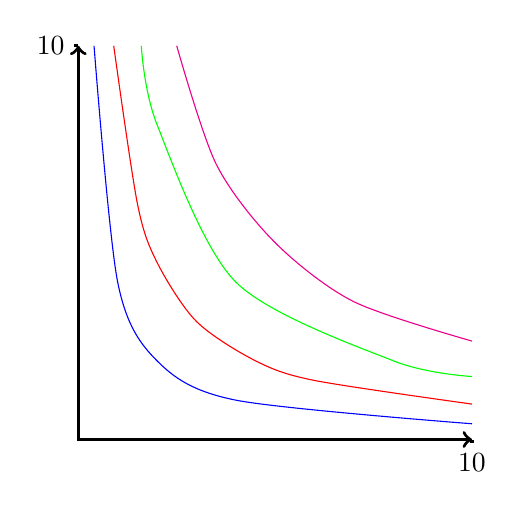
\begin{tikzpicture}[scale = 0.5]
            \draw[<->,very thick] (0,10)--(0,0)--(10,0);
            \draw [blue] plot [smooth, tension=0.5] coordinates { (0.4,10) (1,4) (2,2) (4,1) (10,0.4) };
            \draw [red] plot [smooth, tension=0.5] coordinates { (0.9,10) (1.5,6) (2,4.5) (3,3) (4.5,2) (6,1.5) (10,0.9) };
            \draw [green] plot [smooth, tension=0.5] coordinates { (1.6,10) (2,8) (4,4) (8,2) (10,1.6) };
            \draw [magenta] plot [smooth, tension=0.5] coordinates { (2.5,10) (3.5,7) (5,5) (7,3.5) (10,2.5) };

            \node [left] at (-0.1,10) {10};
            \node [below] at (10,-0.1) {10};
            \draw[very thick] (0,10)--(-0.1,10);
            \draw[very thick] (10,0)--(10,-0.1);
        \end{tikzpicture}
        \caption{Indifference Curves for $u(x,y) = x^\alpha y^{1-\alpha}$ at $u = \{\textcolor{blue}{2},\textcolor{red}{3},\textcolor{green}{4},\textcolor{magenta}{5}\}$ and $\alpha = 0.5$}
        \label{fig:prob1a}
    \end{figure}
    
    
    First, note that if a bundle $(x,y)$ maximizes $u(x,y)$, it would also maximize $\ln u(x,y)$, so we will deal with the second problem. We have that $\ln u(x,y) = \alpha \ln x + (1 - \alpha) \ln y$. The Lagrangian is
    \[
    \mathcal{L} = \alpha \ln x + (1 - \alpha) \ln y + \lambda (w - p_xx - p_yy)
    \]
    The first order conditions are
    \[
    \mathcal{L}_x = \frac{\alpha}{x} - p_x \lambda = 0 \Rightarrow p_x = \frac{\alpha}{\lambda x} \Rightarrow x = \frac{\alpha}{p_x \lambda}
    \]
    \[
    \mathcal{L}_y = \frac{1-\alpha}{y} - p_y \lambda = 0 \Rightarrow p_y = \frac{1-\alpha}{\lambda y} \Rightarrow y = \frac{1-\alpha}{p_y \lambda}
    \]
    Substituting into the budget constraint, we get
    \[
    \frac{\alpha}{\lambda x} x + \frac{1-\alpha}{\lambda y} y = \frac{\alpha}{\lambda} + \frac{1-\alpha}{\lambda} = \frac{1}{\lambda} = w \Rightarrow \lambda = \frac{1}{w}
    \]
    Plugging this result back in, we get the Marshallian demand functions
    \[
    \boxed{x^*(p,w) = \frac{w\alpha}{p_x} \;\;\;;\;\;\; y^*(p,w) = \frac{w(1-\alpha)}{p_y}}  
    \]
    Substituting these into the utility function will give us the indirect utility function
    \[
    \boxed{v(p,w) = u(x^*(p,w),y^*(p,w)) = w\left(\frac{\alpha}{p_x} \right)^\alpha \left(\frac{1-\alpha}{p_y} \right)^{1-\alpha}}
    \]
    To find the expenditure function, we substitute into the indirect utility function
    \[
    \overline{u} = e(p,\overline{u})\left(\frac{\alpha}{p_x} \right)^\alpha \left(\frac{1-\alpha}{p_y} \right)^{1-\alpha}
    \]
    and get
    \[
    \boxed{e(p,\overline{u}) = \overline{u} \left(\frac{p_x}{\alpha} \right)^{\alpha} \left(\frac{p_y}{1-\alpha} \right)^{1-\alpha}}
    \]
    Finally, by Shephard's Lemma we know that $\nabla_p e = h$. By taking the partial derivatives, we get that
    \[
    \boxed{h_x(p,\overline{u}) = \alpha \overline{u} \left(\frac{p_x}{\alpha} \right)^{\alpha-1} \left(\frac{p_y}{1-\alpha} \right)^{1-\alpha}}
    \]
    \[
    \boxed{h_y(p,\overline{u}) = (1-\alpha) \overline{u} \left(\frac{p_x}{\alpha} \right)^{\alpha} \left(\frac{p_y}{1-\alpha} \right)^{-\alpha}}
    \]
    

    \item[(b)] The indifference curves are:

    \begin{figure}[H]
        \centering
        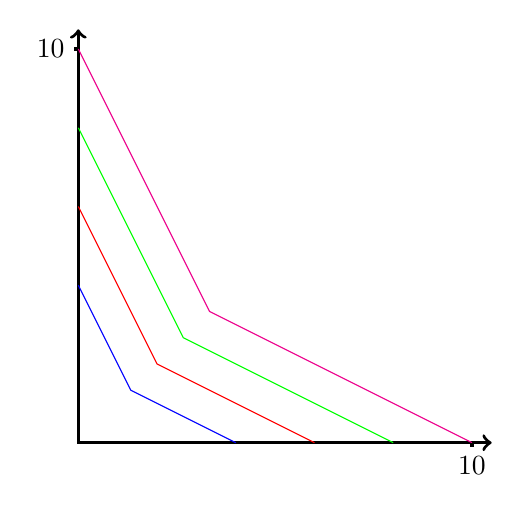
\begin{tikzpicture}[scale = 0.5]
            \draw[<->,very thick] (0,10.5)--(0,0)--(10.5,0);
            \draw [blue] (0,4)--(4/3,4/3)--(4,0);
            \draw [red] (0,6)--(2,2)--(6,0);
            \draw [green] (0,8)--(8/3,8/3)--(8,0);
            \draw [magenta] (0,10)--(10/3,10/3)--(10,0);
            \node [left] at (-0.1,10) {10};
            \node [below] at (10,-0.1) {10};
            \draw[very thick] (0,10)--(-0.1,10);
            \draw[very thick] (10,0)--(10,-0.1);
        \end{tikzpicture}
        \caption{Indifference Curves for $u(x,y) = \max\{a x,ay\} + \min\{x,y\}$ at $u = \{\textcolor{blue}{2},\textcolor{red}{3},\textcolor{green}{4},\textcolor{magenta}{5}\}$ and $a = 0.5$}
        \label{fig:prob1a}
    \end{figure}
    
    
    
    Without loss of generality, assume that $p_x \le p_y$. Note that $u(x,y) = u(y,x)$ for all $x,y$, which means that $h_x(p,\overline{u}) \ge h_y(p,\overline{u})$. To see why, consider that if $x < y$ and $u(x,y) \ge \overline{u}$, then $u(y,x) \ge \overline{u}$, but since $p_xx+p_yy > p_xy + p_yx$, the expenditure function would not be minimized. Thus, $h_x(p,\overline{u}) \ge h_y(p,\overline{u})$. This means that the expenditure minimization problem will be
    \[
    \begin{array}{ll}
        \min_{x,y \ge 0 ; x \ge y} & p_xx + p_yy \\
        \text{subject to} & ax + y \ge \overline{u}
    \end{array}
    \]
    Since the objective and constraint are both linear, we will always have a corner solution:

    If $a > \frac{p_x}{p_y}$, the optimal solution will have $y = 0$, so $h_x(p,\overline{u}) = \frac{\overline{u}}{p_x}$, $h_y(p,\overline{u}) = 0$, and $e(p,\overline{u}) = \overline{u}\frac{p_x}{a}$. Additionally, $x^*(p,w) = \frac{w}{p_x}$ and $y^*(p,w) = 0$, meaning that $v(p,w) = \frac{aw}{p_x}$.

    If $a < \frac{p_x}{p_y}$, the optimal solution will have $x = y$, so $h_x(p,\overline{u}) = h_y(p,\overline{u}) = \frac{\overline{u}}{a+1}$, and $e(p,\overline{u}) = \overline{u}\frac{p_x + p_y}{a+1}$. Additionally, $x^*(p,w) = \frac{w}{p_x + p_y} = y^*(p,w)$, so $v(p,w) = \frac{w(a+1)}{p_x + p_y}$.

    If $a = \frac{p_x}{p_y}$, any solution where $x \ge y \ge 0$ will be optimal as long as $ax + y = \overline{u}$. This means that $h(p,\overline{u}) = \{(x,y) : x \ge y \ge 0 \text{ and } ax + y = \overline{u}\}$, and $e(p,\overline{u}) = \overline{u}\frac{p_x + p_y}{a+1} = \overline{u}\frac{p_x}{a}$. Additionally, $(x^*(p,w),y^*(p,w)) = \{(x,y) : x \ge y \ge 0 \text{ and } ax + y = \frac{aw}{p_x}\}$, so $v(p,w) = \frac{aw}{p_x}$.

    All of these results of course hold in the other direction if $p_x > p_y$.
    
\end{itemize}

\paragraph{Problem 2:} Consider an expenditure function of the following form:
\[
e(p,u) = \exp\left(\sum_l \alpha_l \log p_l + u\prod_l p_l^{\beta_l}  \right)
\]
\begin{itemize}
    \item[(a)] What conditions must parameters $\alpha_1,\dots,\alpha_n$, $\beta_1,\dots,\beta_n$ satisfy for this expenditure function to be rationalizable?
\end{itemize}


\noindent From now on, assume the restrictions in (a) are satisfied


\begin{itemize}
    \item[(b)] Derive the consumer's Hicksian and Marshallian demand functions. 

    \item[(c)] Check whether the different goods are substitutes or complements, and whether they are gross substitutes or gross complements. Interpret.

    \item[(d)] What utility function rationalizes this expenditure function? [Hint: for an inner bound on an indifference curve you can combine the Hicksian demands for the different goods in a way that eliminates the prices.]
\end{itemize}

\medskip

\textbf{Solutions:}

\begin{itemize}
    \item[(a)] For this expenditure function to be rationalizable, it suffices to show that it meets three conditions: nondecreasing in $p$, homogeneous of degree 1 in $p$, and concave in $p$. We will address these conditions in order.

    \smallskip

    For $e(p,u)$ to be nondecreasing in $p$, the partial derivative $\partial e(p,u) / \partial p_i$ must be non-negative for each $p_i$. Taking the derivative, we get
    \[
    \frac{\partial e(p,u)}{\partial p_i} = \left(\frac{\alpha_i}{p_i} + u\beta_i p_i^{\beta_i - 1} \prod_{l\ne i} p_l^{\beta_l} \right) e(p,u)
    \]
    As the expenditure function is positive, for this to be true for all $i,p,u$ it must be the case that $\beta_i \ge 0$ and $\alpha_i \ge 0$ for all $i$.

    \smallskip

    For $e(p,u)$ to be homogeneous of degree 1 in $p$, it must be the case that $e(\lambda p,u) = \lambda e(p,u)$. Expanded, this is
    \begin{align*}
        e(\lambda p,u) &= \exp\left(\sum_l \alpha_l \log \lambda p_l + u\prod_l (\lambda p_l)^{\beta_l}  \right) \\
        &= \lambda^{\sum_l \alpha_l} \exp\left(\sum_l \alpha_l \log p_l + \lambda^{\sum_l \beta_l} u\prod_l p_l^{\beta_l}  \right)
    \end{align*}
    which equals $\lambda e(p,u)$ only when $\sum_l \alpha_l = 1$ and $\sum_l \beta_l = 0$. Since $\beta_l \ge 0$ for all $l$, $\beta_l = 0$ for all $l$. This means that the expenditure function simplifies to
    \[
    e(p,u) = \exp\left(\sum_l \alpha_l \log p_l + u \right) = e^u \prod_l p_l^{\alpha_l}
    \]

    \smallskip

    Our final condition is that $e(p,u)$ is concave. It suffices to show that $\partial^2 e(p,u) / \partial p_i^2 \le 0$ for all $p_i$, which is equivalent to the elements of the diagonal of the Slutsky matrix being non-positive. We have
    \[
    \frac{\partial^2 e(p,u)}{\partial p_i^2} = e^u \alpha_i (\alpha_i - 1) p_i^{\alpha_i - 2} \prod_{l \ne i} p_l^{\alpha_l}
    \]
    All of the terms are nonnegative by assumption except for $\alpha_i - 1$. Since $\alpha_i \ge 0$ for all $i$, for $e(p,u)$ to be concave, it must be the case that $\alpha_i \in [0,1]$ for all $i$.

    \smallskip

    Thus, the conditions for the expenditure function to be rationalizable are that $\beta_i = 0$ for all $i$, that $\alpha_i \in [0,1]$ for all $i$, and that $\sum_i \alpha_i = 1$.

    \item[(b)] Since the restrictions are satisfied, we will use the more simple form for the expenditure function. Using Shephard's Lemma, we find that the Hicksian demand functions are
    \[
    h_i(p,u) = \nabla_{p_i} e(p,u) = e^u \alpha_i p_i^{\alpha_i - 1} \prod_{l \ne i} p_l^{\alpha_l} = \frac{e^u \alpha_i}{p_i} \prod_{l} p_l^{\alpha_l}
    \]
    To find Marshallian demand, we use the identity that $h_i(p,u) = x_i(p,e(p,u))$. Note that $h_i(p,u) = \frac{\alpha_i}{p_i} e(p,u)$. Thus, $x_i(p,w) = \frac{\alpha_i w}{p_i}$.

    \item[(c)] To find whether two goods are substitutes of complements, we take the partial of the Hicksian demand for one good with respect to the price of the other:
    \[
    \frac{\partial h_i(p,u)}{\partial p_j} = e^u \frac{\alpha_i \alpha_j}{p_ip_j} \prod_{l} p_l^{\alpha_l}
    \]
    Since all terms are non-negative, two different goods are substitutes.

    \smallskip

    To find whether two goods are gross substitutes or gross complements, we take the partial of the Marshallian demand for one good with respect to the price of the other:
    \[
    \frac{\partial x_i(p,w)}{\partial p_j} = 0
    \]
    Since the total effect is 0, the goods are neither strict gross complements nor strict gross substitutes. This means that when the price of one good increases, the consumer will substitute away from that good to others, but this substitution will be offset by a wealth effect, so the total effect on demand will be nothing.

    \item[(d)] Note first that the Marshallian demand function looks exactly the same as the Marhsallian demand developed from a Cobb-Douglas utility function in Problem 1. A reasonable choice of utility function is
    \[
    u(x) = \sum_l \alpha_l (\ln x_l + \ln \alpha_l)
    \]
    To check that this utility function rationalizes the expenditure function, we will use it to derive Hicksian demand. Our expenditure minimization problem is
    \[
    \min_{\sum_l \alpha_l (\ln x_l + \ln \alpha_l) \ge \overline{u}} \sum_i p_ix_i
    \]
    The first order conditions imply that $-\lambda = \frac{p_ix_i}{\alpha_i}$. Fixing $i = 1$, note that we can now write $x_i = \frac{p_1x_1\alpha_i}{\alpha_1 p_i}$, and solve for the Hicksian demand:
    \begin{align*}
        \overline{u} &= \sum_l \alpha_l (\ln \frac{p_1x_1\alpha_i}{\alpha_1 p_i} + \ln \alpha_l) \\
        \Longrightarrow e^{\overline{u}} &= \frac{x_1p_1}{\alpha_1} \prod_l p_l^{\alpha_l} \\
        \Longrightarrow h_1(p,\overline{u}) &= \frac{e^{\overline{u}}\alpha_1}{p_1}\prod_l p_l^{\alpha_l}
    \end{align*}
    Since that is the Hicksian demand found above, the utility function that rationalizes the expenditure function is
    \[
    u(x) = \sum_l \alpha_l (\ln x_l + \ln \alpha_l)
    \]
\end{itemize}

\paragraph{Problem 3:} Let the consumption set be $\reals \times \reals_+^{n-1}$, and suppose that preferences are strictly convex and quasi-linear in the first good (``numeraire''). (Note that negative consumption of numeraire is allowed.) Fix the numeraire's price $p_1 = 1$.

\begin{itemize}
    \item[(a)] Show that the Marshallian demand functions for goods $2,\dots,n$ are independent of wealth. 

    \item[(b)] Show that the Hicksian demand functions for goods $2,\dots,n$ are independent of target utility.

    \item[(c)] What does this imply about the relationship between Marshallian and Hicksian demand for goods $2,\dots,n$?

    \item[(d)] Argue that the consumer's preferences over $(p,w)$ can be represented by an indirect utility function that is quasilinear in $w$. What is the form of the corresponding expenditure function?

    \item[(e)] Compare (i) compensating variation, (ii) equivalent variation, and (iii) consumer surplus calculated from Marshallian demand to each other.
\end{itemize}

\medskip

\textbf{Solutions:}

\begin{itemize}
    \item[(a)] Recall that if a consumer is maximizing a quasilinear utility function, there exists a utility representation $U$ such that $U(x) = x_1 + u(x_2,\dots,x_n)$. Note that since utility is increasing in $x_1$, the budget constraint will hold with equality by Walras' Law. Solving for $x_1$ in the budget constraint, we get $x_1 = w - p_2x_2 - \dots - p_nx_n$. The consumer's utility maximization problem
    \[
    \max_{x_1 + p_2x_2 + \dots + p_nx_n = w} U(x)
    \]
    Is equivalent to the unconstrained problem
    \[
    \max_{x_2,\dots,x_n} w + u(x_2,\dots,x_n) - p_2x_2 - \dots - p_nx_n
    \]
    Which is equivalent to
    \[
    w + \max_{x_2,\dots,x_n} u(x_2,\dots,x_n) - p_2x_2 - \dots - p_nx_n
    \]
    Since the solutions to this problem, which are the Marshallian demand functions, are independent of wealth, the Marshallian demand functions for goods $2,\dots,n$ are independent of wealth.
    

    \item[(b)] From the definition of the indirect utility function and part (a), we know that 
    \[
    v(p,w) = w + \max_{x_2,\dots,x_n} u(x_2,\dots,x_n) - p_2x_2 - \dots - p_nx_n
    \]
    To find the expenditure function, we set $v(p,e(p,\overline{u})) = \overline{u}$
    \[
    \overline{u} = e(p,\overline{u}) + \max_{x_2,\dots,x_n} u(x_2,\dots,x_n) - p_2x_2 - \dots - p_nx_n
    \]
    Thus, the expenditure function is
    \[
    e(p,\overline{u}) = \overline{u} - \max_{x_2,\dots,x_n} u(x_2,\dots,x_n) - p_2x_2 - \dots - p_nx_n
    \]
    From Shephard's Lemma, the Hicksian demand is
    \[
    h_i(p,u) = \nabla_{p_i} e(p,u) = -\frac{\partial}{\partial p_i}\left(\max_{x_2,\dots,x_n} u(x_2,\dots,x_n) - p_2x_2 - \dots - p_nx_n\right)
    \]
    Thus, Hicksian demand is independent of target utility.

    \item[(c)] Since Marshallian demand is independent of wealth, the Slutsky Equation is
    \[
    \frac{\partial x_i(p,w)}{\partial p_j} = \frac{\partial h_i(p,\overline{u})}{\partial p_j}
    \]
    Since $x_i(p,0) = 0$, $h_i(p,v(p,0)) = 0$. Since the two forms of demand have the same starting condition and the same slope at every point, we can say that $x_i(p,w) = h_i(p,\overline{u})$ for all $i \ge 2$.

    \item[(d)] Define a function
    \[
    \psi(p) = \max_{x_2,\dots,x_n} u(x_2,\dots,x_n) - p_2x_2 - \dots - p_nx_n
    \]
    We have already shown in part (b) that
    \[
    v(p,w) = w + \psi(p)
    \]
    and
    \[
    e(p,\overline{u}) = \overline{u} - \psi(p)
    \]
    The functions are quasilinear in $w$ and $\overline{u}$ by inspection.

    \item[(e)] From the definitions of compensating and equivalent variation, it is clear to see that
    \[
    CV = e(p,u) - e(p',u) = \psi(p') - \psi(p) = e(p,u') - e(p',u') = EV
    \]
    Since the Marshallian consumer surplus is bounded by compensating variation and equivalent variation, it is equal to both, and the three quantities are equal.

    
\end{itemize}

\paragraph{Problem 4:} Suppose that instead of a fixed wealth, the consumer starts with a bundle of goods $z$ (not necessarily her optimal bundle) and can buy and sell goods at prices $p$. Suppose that all goods are regular. Explain why (or give an example of how) the consumer's demand for good 1 might be higher at prices $p' = (p_1',p_2,\dots,p_n)$ than at prices $p$, with $p_1' > p_1$. What is required for this to happen?

\textbf{Solutions:} Assume that the consumer starts with a positive amount of good 1. Since good 1 is regular, an increase in the price of good 1 while holding wealth constant will decrease demand for good 1. However, since she starts with a positive amount of good 1, the increasing price of good 1 is effectively increasing her wealth, since $w = p\cdot z$ in this example, and $p' \cdot z > p \cdot z$. She will increase her demand for good 1 if good 1 is normal as well as regular, and if the wealth effect is greater in magnitude than the substitution effect. 

\medskip

For an example, consider $u(x_1,x_2) = \min\{x_1,x_2\}$, $z = (3,0)$, $p = (1,1)$, and $p' = (2,1)$. Her demand under $p$ will be $(1.5,1.5)$, and her demand under $p'$ will be $(2,2)$.


\paragraph{Problem 5:} A consumer in a three-good world faces prices $p_1 = p_2 = p_3 = 1$. She buys $x_1 = x_2 = x_3 = 2$. Prices change, and next year she faces prices $p_1 = p_3 = 4$ and $p_2 = 2$. She buys $x_1 = 1$, $x_2 = 2$, and $x_3 = 10$.

\begin{itemize}
    \item[(a)] Construct the Paasche and Laspeyres price indices for this consumer.

    \item[(b)] What can you say about the change in this consumer's welfare?
\end{itemize}
\medskip
\textbf{Solutions:}

\begin{itemize}
    \item[(a)] The Paasche index is
    \[
    \frac{p' \cdot x'}{p \cdot x'} = \frac{4 + 4 + 40}{1 + 2 + 10} = \frac{48}{13} \approx 3.69
    \]
    The Laspeyres index is
    \[
    \frac{p' \cdot x}{p \cdot x} = \frac{8 + 4 + 8}{2 + 2 + 2} = \frac{20}{6}  \approx 3.33
    \]

    \item[(b)] We can see that the consumer spent 48 in the second year, so her wealth must be at least 48. Since the first year's consumption bundle costs 20, it must have been feasible, yet she chose to consume the second year's bundle. This indicates that $u(x') > u(x)$, which means that her welfare increased despite the price indices both indicating that it would require a wealth increase to keep her utility the same. This indicates that her wealth increased from year 1 to year 2, and that increase made her better off despite the price increases.
\end{itemize}

\paragraph{Problem 6:} Suppose there are $m$ consumers, and that the indirect utility function of each consumer $i = 1,\dots,m$ takes the form
\[
v_i(p,w_i) = a_i(p) + b(p)w_i
\]
for some differentiable functions $a_i(\cdot) \; (i = 1,\dots,m)$ and $b(\cdot)$.

\begin{itemize}
    \item[(a)] Show that this form of indirect utility function obtains (for some utility representation of preferences) when either (i) all consumers have quasilinear preferences or (ii) all consumers have identical homothetic preferences.

    \item[(b)] Show that the consumers' aggregate demand
    \[
    X(p,w_1,\dots,w_m) = \sum_{i=1}^m x_i(p,w_i)
    \]
    can be written as $X(p,W)$, where $W = \sum_{i=1}^m w_i$ is the aggregate wealth.

    \item[(c)] Show, moreover, that $X(p,W)$ can arise as the Marshallian demand function of a single utility-maximizing consumer (interpreted as the ``positive representative consumer''). [Hint: show that the demand can be derived from an expenditure function that is rationalizable.]

    \item[(d)] Show that a change in prices makes the ``representative consumer'' better off if and only if there exists an accompanying redistribution of the aggregate wealth that would make each consumer $i = 1,\dots,m$ better off. (Thus we also have a ``normative representative consumer.'')
\end{itemize}

\textbf{Solutions:}

\begin{itemize}
    \item[(a)] First, assume that all consumers have quasilinear preferences. Normalize $p_1 = 1$. From Problem 3, we know that our value function becomes
    \[
    v^i(p,w_i) = \max_{x_{-1} \ge 0} w_i - p_{-1}\cdot x_{-1} + u(x_{-1})
    \]
    where $x_{-1} = (x_2,\dots,x_n)$. Since demand does not depend on $w_i$, we can define $x_{-1}^*(p)$ as the demand for all non-numeraire goods. Because Walras' Law holds, our budget constraint is an equality constraint, so we have $x^*(p,w) = w - p_{-1} \cdot x^*_{-1}(p)$. Finally, our value function becomes $v^i(p,w_i) = w_i - p_{-1}\cdot x^*_{-1}(p) + u(x_{-1}^*(p))$. This matches the form above, where $b(p) = 1$ and $a_i(p) = - p_{-1}\cdot x^*_{-1}(p) + u(x_{-1}^*(p))$.

    \smallskip

    Next, assume that all consumers have identical homothetic preferences. From the first problem set, there exists $u(x)$ that is homogeneous of degree 1. Using that function, which is identical across all consumers, the value function is
    \begin{align*}
        v^i(p,w_i) &= \max_{x ; x\cdot p \le w_i} u(x) \\
                &= \max_{z ; z\cdot p \le 1} u(w_iz) \text{  for } z = \frac{x}{w_i} \\
                &= w_i \max_{z ; z\cdot p \le 1} u(z) \\
                &= w_i v(p,1)
    \end{align*}
    Thus, setting $a_i(p) = 0$ and $b(p) = v(p,1)$, we have a solution.

    \item[(b)] From Roy's Identity, we have that $\nabla v^i(p,w_i) = x^i(p,w_i)$. Using that, we get
    \begin{align*}
        X(p,w_1,\dots,w_n) &= \sum_{i=1}^m x^i(p,w_i) \\
        &= \nabla \sum_{i=1}^m v^i(p,w_i) \\
        &= \nabla \sum_{i=1}^m a^i(p) + b(p)w_i \\
        &= W\nabla b(p) + \sum_{i=1}^m \nabla a^i(p) \\
        &= X(p,W)
    \end{align*}

    \item[(c)] We begin by calculating the individual expenditure functions using the identity $v(p,e) = \overline{u}$:
    \[
    v^i(p,e^i(p,u^i)) = u^i = a^i(p) + b(p)e^i(p,u^i) \Longrightarrow e^i(p,u^i) = \frac{u^i - a^i(p)}{b(p)}
    \]
    We then aggregate, defining $a(p) = \sum_i a^i(p)$ and $U = \sum_i u^i$, and get
    \[
    e(p,U) = \frac{U - a(p)}{b(p)}
    \]
    To find the aggregate Marshallian demand, we first find the aggregate indirect utility function
    \[
    W = \frac{v(p,W) - a(p)}{b(p)} \Longrightarrow v(p,W) = a(p) + Wb(p)
    \]
    Finally, using Roy's Identity we can identify the representative consumer's aggregate demand
    \[
    X(p,W) = -\frac{-\nabla_p v(p,W)}{\partial v(p,W) / \partial W} = -\frac{\nabla_p a(p) + W\nabla_p b(p)}{b(p)} 
    \]
    \[
    X(p,W) = \sum_i -\frac{\nabla_p a_i(p) + w_i\nabla_p b(p)}{b(p)}
    \]
    This represents the Marshallian demand for a rational representative consumer.

    \item[(d)] 

    \begin{proof}
        $(\Rightarrow)$: Assume that we have a price change $p \to p'$ which makes the representative agent better off, meaning that $v(p',W) > v(p,W)$, and we have a possible wealth redistribution $w \to w'$. For each agent to be better off, we need
        \[
        v_i(p',w_i') = a_i(p') + b(p')w'_i \ge a_i(p) + b(p)w_i = v_i(p',w_i)
        \]
        This means the redistribution must be
        \[
        w'_i \ge \frac{a_i(p) - a_i(p') + b(p)w_i}{b(p')}
        \]
        Assume that this holds with equality, meaning that each agent is compensated so that they are the same as before the price change. To find if this is feasible, using the fact that the representative consumer is better off, we find
        \[
        \sum_i w_i' = \frac{v(p,W) - a_i(p')}{b(p')} \le \frac{v(p',W) - a_i(p')}{b(p')} = \sum_i w_i = W
        \]
        Thus, since a redistribution making each agent better off is feasible, a change in prices which makes the representative consumer better off implies that there exists an accompanying redistribution of the aggregate wealth that makes each consumer better off.

        \medskip

        $(\Leftarrow)$: Assume that we have a price change $p \to p'$ and an accompanying wealth redistribution $w_i \to w_i'$ such that each agent is better off. That implies that 
        \[
        v_i(p',w_i') = a_i(p') + b(p')w_i' \ge a_i(p) + b(p)w_i = v_i(p,w_i)
        \]
        Summing as in part (c), and recalling that $\sum_i w_i = \sum_i w'_i = W$, since we are redistributing, we get
        \[
        v(p',W) = a(p') + b(p')W \ge a(p) + b(p)W = v(p,W)
        \]
        Since $v(p',W) \ge v(p,W)$, the representative agent is better off.
    \end{proof}

    
\end{itemize}


\newpage
\subsection{Producer (Harris)}

\subsubsection{Harris Homework}

\paragraph{Problems.}

\begin{enumerate}
	\item Consider the production possibilities set
	\[
	Y = \curll (q,-z) \in \reals^2_+ \times \reals^2_- : z_1^\alpha z_2^\beta \ge \frac{q_1^2 + q_2^2}{2} \curlr
	\]
	where $\alpha,\beta > 0$.
	\begin{enumerate}
		\item Find the conditional input demand function $z(w_1,w_2,q_1,q_2)$.
		\item What is the marginal rate of transformation between output 1 and output 2? That is, given $w_1, w_2, q_1, q_2$, what is the proportional decrease in $q_1$ required to marginally increase $q_2$ while holding cost constant?
	\end{enumerate}
	\item Consider a single-output firm with technology that can transform inputs $z \in \reals^3_+$ into output according to the production function
	\[
	f(z) = z_1^\frac{1}{2} z_2^\frac{1}{4} z_3^\frac{1}{8}
	\]
	\begin{enumerate}
		\item This production function is homogeneous degree $\alpha$. Find $\alpha$. What does this imply about the firm’s cost function? Is the firm’s marginal cost of production increasing or decreasing in $q$?
		\item Derive the conditional input demand function $z(w, q)$.
		\item Derive an expression for the firm’s marginal cost of production, i.e., the derivative of the cost function with respect to $q$.
	\end{enumerate}
	\item Consider a single- output firm which takes as input a continuum of inputs rather than a discrete set of inputs. We now denote the quantity input of commodity $j$ as $z(j)$ (rather than $z_j$ as we did in the discrete-inputs cases). The production function is
	\[
	f(z) = \barl \int_0^1 a(j) z(j)^{\frac{\sigma-1}{\sigma}} dj \barr^{\frac{\sigma}{\sigma-1}} 
	\]
	where $a(j)$ is a continuous function integrable on $[0, 1]$ that reflects the relative productivities of the various inputs.
	\begin{enumerate}
		\item Derive the conditional input demand function $z(j, w, q)$. The price for input $j$ is given by $w(j)$, where $w$ is a continuous function integrable on $[0, 1]$.
		\item How is the conditional input demand for input $j$ affected by $a(j)$, the productivity of input $j$?
		\item N0w suppose that the firm has market power in input markets. If the firm uses $z(j)$ units of input $j$, the per-unit input price is $w(j,z(j)) = \frac{1}{2} z(j)$. Find the cost-minimizing choice of inputs to produce $q = 1$ units of output.
	\end{enumerate}
	\item Consider a single-output firm with technology that can transform inputs $z \in \reals^N_+$ into output according to the production function
	\[
	f(z) = 2\sqrt{\min\{z_1,2z_2,3z_3,\dots,Nz_N}
	\]
	\begin{enumerate}
		\item Derive the unconditional input demand function.
		\item ow suppose that the firm has market power in the output market. If the firm produces quantity $q$, the per-unit price is $P(q) = q^{-\varepsilon}$ where $\varepsilon \in (1,\infty)$. Derive the firm's choice of inputs $z_1,\dots,z_N$.
	\end{enumerate}
	\item De Loecker, Eeckhout, and Unger (QJE, 2020) is an influential paper on measuring market power. The approach described in this paper takes the cost minimization problem as a starting point. Read the first 11 pages of this article (through the end of Section II.B) paying particular attention to Sections II.A and II.B.
	\begin{enumerate}
		\item In going from equation (6) to (7), the authors assert that ``The La- grange multiplier $\lambda$ is a direct measure of marginal cost.'' Give a justification for this assertion.
		\item The authors’ starting point in Section II.B is the cost minimiza- tion problem. However, the output price (the key component of the markup) does not feature in the CMP (recall that the only arguments of the cost function and conditional input demand function are $w$ and $q$). Given this, why can the authors claim that this starting point leads to some insight about markups? Wouldn’t it be more natural to use the profit maximization problem as a starting point?
	\end{enumerate}
\end{enumerate}

\paragraph{Solutions.} (Gabe's solutions, collaborated with Sara Yoo)

\begin{enumerate}
	\item Production possibilities set
	\begin{enumerate}
		\item We have that the cost minimization problem is
		\[
		\min_{z\in \reals^2_+} w_1z_1 + w_2z_2 \st z_1^\alpha z_2^\beta \ge \frac{q_1^2 + q_2^2}{2}
		\]
		Which has the Lagrangian
		\[
		\mathcal{L} = w_1 z_1 + w_2 z_2 + \lambda \parl  \frac{q_1^2 + q_2^2}{2} -  z_1^\alpha z_2^\beta\parr
		\]
		Taking first order conditions, we get
		\[
		\frac{\partial \mathcal{L}}{\partial z_1} = w_1 - \lambda \alpha z_2^\beta z_1^{\alpha - 1} = 0 \Longrightarrow \lambda = \frac{w_1}{\alpha z_2^\beta z_1^{\alpha - 1}} 
		\]
		\[
		\frac{\partial \mathcal{L}}{\partial z_2} = w_2 - \lambda \beta z_1^\alpha z_2^{\beta - 1} = 0 \Longrightarrow \lambda = \frac{w_2}{\beta z_1^\alpha z_2^{\beta - 1}}
		\]
		\[
		\frac{\partial \mathcal{L}}{\partial \lambda} = \frac{q_1^2 + q_2^2}{2} -  z_1^\alpha z_2^\beta = 0 \Longrightarrow \frac{q_1^2 + q_2^2}{2} =  z_1^\alpha z_2^\beta
		\]
		Combining, we get that
		\[
		\frac{w_1}{\alpha z_2^\beta z_1^{\alpha - 1}} = \frac{w_2}{\beta z_1^\alpha z_2^{\beta - 1}} \Longrightarrow \frac{w_1 z_1}{\alpha} = \frac{w_2 z_2}{\beta} \Longrightarrow z_1 = \frac{w_2\alpha}{w_1\beta} z_2
		\]
		Substituting into the constraint, we get that
		\begin{align*}
			\parl \frac{w_2\alpha}{w_1\beta} z_2 \parr^\alpha z_2^\beta &= \frac{q_1^2 + q_2^2}{2} \\
			z_2^{\alpha + \beta} &= \parl \frac{w_1\beta}{w_2\alpha}\parr^{\alpha} \frac{q_1^2 + q_2^2}{2} \\
			z_2\opt(w_1,w_2,q_1,q_2) &= \parl \frac{w_1\beta}{w_2\alpha}\parr^{\frac{\alpha}{\alpha + \beta}} \parl\frac{q_1^2 + q_2^2}{2}\parr^{\frac{1}{\alpha + \beta}}
		\end{align*}
		Substituting back into the equation for $z_1$, we get that
		\begin{align*}
			z_1 &=  \frac{w_2\alpha}{w_1\beta} \parl \frac{w_1\beta}{w_2\alpha}\parr^{\frac{\alpha}{\alpha + \beta}} \parl\frac{q_1^2 + q_2^2}{2}\parr^{\frac{1}{\alpha + \beta}} \\
			z_1\opt(w_1,w_2,q_1,q_2) &= \parl \frac{w_2\alpha}{w_1\beta} \parr^{\frac{\beta}{\alpha + \beta}}\parl\frac{q_1^2 + q_2^2}{2}\parr^{\frac{1}{\alpha + \beta}}
		\end{align*}
		\item We can find the Marginal Rate of Transformation by implicitly differentiating the border of the production possibilities set. More specifically, since we have that price must remain constant, we have that
		\[
		0 = 2q_1 \partial q_1 + 2q_2 \partial q_2 \Longrightarrow MRT_{q_1,q_2} = \frac{\partial q_1}{\partial q_2} = -\frac{q_2}{q_1}
		\]
	\end{enumerate}
	\item Cost minimization
	\begin{enumerate}
		\item We have that the production function is homogeneous of degree $\alpha$, meaning that $f(\beta z) = \beta^\alpha f(z)$. We have that
		\[
		f(\beta z) = \parl \beta z_1\parr^{\frac{1}{2}} \parl \beta z_2\parr^{\frac{1}{4}} \parl \beta z_3\parr^{\frac{1}{8}} = \beta^{\frac{7}{8}} z_1^{\frac{1}{2}} z_2^{\frac{1}{4}} z_3^{\frac{1}{8}} = \beta^{\frac{7}{8}} f(z)
		\]
		so $\alpha = \frac{7}{8}$. This implies that the firm's cost function is homogeneous of degree $\frac{8}{7}$ in $q$, which implies that the firm faces increasing marginal cost of production in $q$.
		\item We have that the cost minimization problem is
		\[
		\min_{z \in \reals^3_+} w \cdot z \st z_1^{\frac{1}{2}} z_2^{\frac{1}{4}} z_3^{\frac{1}{8}} \ge q
		\]
		which admits the Lagrangian
		\[
		\mathcal{L} =  w \cdot z + \lambda \parl q - z_1^{\frac{1}{2}} z_2^{\frac{1}{4}} z_3^{\frac{1}{8}} \parr
		\]
		Our first order conditions are
		\[
		\frac{\partial \mathcal{L}}{\partial z_1} = w_1 - \frac{\lambda}{2} z_1^{-\frac{1}{2}} z_2^{\frac{1}{4}} z_3^{\frac{1}{8}} = 0 \Longrightarrow \lambda = \frac{2w_1 }{ z_1^{-\frac{1}{2}} z_2^{\frac{1}{4}} z_3^{\frac{1}{8}}}
		\]
		\[
		\frac{\partial \mathcal{L}}{\partial z_2} = w_2 - \frac{\lambda}{4} z_1^{\frac{1}{2}} z_2^{-\frac{3}{4}} z_3^{\frac{1}{8}} = 0 \Longrightarrow \lambda = \frac{4w_2 }{z_1^{\frac{1}{2}} z_2^{-\frac{3}{4}} z_3^{\frac{1}{8}}}
		\]
		\[
		\frac{\partial \mathcal{L}}{\partial z_3} = w_3 - \frac{\lambda}{8} z_1^{\frac{1}{2}} z_2^{\frac{1}{4}} z_3^{-\frac{7}{8}} = 0 \Longrightarrow \lambda = \frac{8w_3 }{z_1^{\frac{1}{2}} z_2^{\frac{1}{4}} z_3^{-\frac{7}{8}}}
		\]
		\[
		\frac{\partial \mathcal{L}}{\partial \lambda} =  q - z_1^{\frac{1}{2}} z_2^{\frac{1}{4}} z_3^{\frac{1}{8}} = 0 \Longrightarrow  q = z_1^{\frac{1}{2}} z_2^{\frac{1}{4}} z_3^{\frac{1}{8}}
		\]
		Equating the first two conditions, we get that
		\[
		\frac{2w_1 }{ z_1^{-\frac{1}{2}} z_2^{\frac{1}{4}} z_3^{\frac{1}{8}}} = \frac{4w_2 }{z_1^{\frac{1}{2}} z_2^{-\frac{3}{4}} z_3^{\frac{1}{8}}} \Longrightarrow z_1w_1 = 2w_2 z_2 \Longrightarrow z_2 = \frac{w_1}{2w_2}z_1
		\]
		Equating the first and third conditions, we get that
		\[
		\frac{2w_1 }{ z_1^{-\frac{1}{2}} z_2^{\frac{1}{4}} z_3^{\frac{1}{8}}} = \frac{8w_3 }{z_1^{\frac{1}{2}} z_2^{\frac{1}{4}} z_3^{-\frac{7}{8}}} \Longrightarrow z_1w_1 = 4w_3 z_3 \Longrightarrow z_3 = \frac{w_1}{4w_3} z_1
		\]
		Combining into the constraint, we get that
		\[
		q = z_1^{\frac{1}{2}} \parl \frac{w_1}{2w_2}z_1\parr^{\frac{1}{4}} \parl \frac{w_1}{4w_3} z_1\parr^{\frac{1}{8}} \Longrightarrow z_1^{\frac{7}{8}}= q \parl \frac{2w_2}{w_1} \parr^\frac{1}{4}  \parl \frac{4w_3}{w_1} \parr^\frac{1}{8} 
		\]
		Which implies that
		\[
		z_1\opt(w,q) = q^\frac{8}{7} \parl \frac{2w_2}{w_1} \parr^\frac{2}{7}  \parl \frac{4w_3}{w_1} \parr^\frac{1}{7}
		\]
		Substituting back, we get that
		\[
		z_2 = \frac{w_1}{2w_2} q^\frac{8}{7} \parl \frac{2w_2}{w_1} \parr^\frac{2}{7}  \parl \frac{4w_3}{w_1} \parr^\frac{1}{7}
		\]
		and
		\[
		z_3 = \frac{w_1}{4w_3} q^\frac{8}{7} \parl \frac{2w_2}{w_1} \parr^\frac{2}{7}  \parl \frac{4w_3}{w_1} \parr^\frac{1}{7}
		\]
		which imply that
		\[
		z_2\opt(w,q) =  q^\frac{8}{7} \parl \frac{w_1}{2w_2} \parr^\frac{5}{7}  \parl \frac{4w_3}{w_1} \parr^\frac{1}{7}
		\]
		\[
		z_3\opt(w,q) =  q^\frac{8}{7} \parl \frac{2w_2}{w_1} \parr^\frac{2}{7} \parl \frac{w_1}{4w_3} \parr^\frac{6}{7}
		\]
		\item We have that the cost function of the firm is $C(w,q) = w_1 z_1\opt + w_2 z_2\opt + w_3z_3\opt$, so substituting:
		\[
		C(w,q) = w_1  q^\frac{8}{7} \parl \frac{2w_2}{w_1} \parr^\frac{2}{7}  \parl \frac{4w_3}{w_1} \parr^\frac{1}{7} + w_2 q^\frac{8}{7} \parl \frac{w_1}{2w_2} \parr^\frac{5}{7}  \parl \frac{4w_3}{w_1} \parr^\frac{1}{7} + w_3 q^\frac{8}{7} \parl \frac{2w_2}{w_1} \parr^\frac{2}{7} \parl \frac{w_1}{4w_3} \parr^\frac{6}{7}
		\]
		which equals
		\[
		C(w,q) = q^\frac{8}{7} \barl w_1  \parl \frac{2w_2}{w_1} \parr^\frac{2}{7}  \parl \frac{4w_3}{w_1} \parr^\frac{1}{7} + w_2 \parl \frac{w_1}{2w_2} \parr^\frac{5}{7}  \parl \frac{4w_3}{w_1} \parr^\frac{1}{7} + w_3  \parl \frac{2w_2}{w_1} \parr^\frac{2}{7} \parl \frac{w_1}{4w_3} \parr^\frac{6}{7}\barr
		\]
		so we have that the marginal cost of production is
		\[
		\frac{\partial C(w,q)}{\partial q} = \frac{8}{7} q^\frac{1}{7} \barl w_1  \parl \frac{2w_2}{w_1} \parr^\frac{2}{7}  \parl \frac{4w_3}{w_1} \parr^\frac{1}{7} + w_2 \parl \frac{w_1}{2w_2} \parr^\frac{5}{7}  \parl \frac{4w_3}{w_1} \parr^\frac{1}{7} + w_3  \parl \frac{2w_2}{w_1} \parr^\frac{2}{7} \parl \frac{w_1}{4w_3} \parr^\frac{6}{7}\barr
		\]
	\end{enumerate}
	\item Cost minimization with a continuum of inputs
	\begin{enumerate}
		\item We have that the continuous cost minimization problem is
		\[
		\min_{z(j)} \int_0^1 w(j)z(j)dj \st q = \barl \int_0^1 a(j) z(j)^\frac{\sigma-1}{\sigma} dj \barr^\frac{\sigma}{\sigma-1}
		\]
		which admits the Lagrangian
		\[
		\mathcal{L} = \int_0^1 w(j)z(j)dj + \lambda \parl q - \barl \int_0^1 a(j) z(j)^\frac{\sigma-1}{\sigma} dj \barr^\frac{\sigma}{\sigma-1} \parr
		\]
		The first order condition with respect to some $z(j)$ is
		\[
		\frac{\partial \mathcal{L}}{\partial z(j)} = w(j) - \lambda \frac{\sigma}{\sigma - 1} \parl \int_0^1 a(i) z(i)^\frac{\sigma - 1}{\sigma}di \parr^\frac{1}{\sigma - 1} \frac{\sigma - 1}{\sigma} a(j) z(j)^{-\frac{1}{\sigma}} = 0
		\]
		and using the fact that $q = \barl \int_0^1 a(j) z(j)^\frac{\sigma-1}{\sigma} dj \barr^\frac{\sigma}{\sigma-1}$ in equilibrium, we get that this simplifies to
		\[
		w(j) - \lambda a(j)z(j)^{-\frac{1}{\sigma}} q^\frac{1}{\sigma} = 0 \Longrightarrow z(j) = \parl \frac{\lambda a(j) q^\frac{1}{\sigma}}{w(j)} \parr^\sigma
		\]
		We can find $\lambda$ by substituting back into the budget constraint:
		\[
		q = \barl\int_0^1 a(j) \parl \frac{\lambda a(j) q^\frac{1}{\sigma}}{w(j)} \parr^{\sigma-1} dj\barr^\frac{\sigma}{\sigma-1} \Longrightarrow q = \barl \lambda^{\sigma - 1}q^\frac{\sigma-1}{\sigma} \int_0^1 a(j)^\sigma w(j)^{1-\sigma} dj \barr^\frac{\sigma}{\sigma - 1}
		\]
		and we get that
		\[
		\lambda\opt = \barl \int_0^1 a(j)^\sigma w(j)^{1-\sigma} dj  \barr^{-\frac{1}{\sigma - 1}}
		\]
		Thus, we have that
		\[
		z\opt(j,w,q) = \parl \frac{a(j)}{w(j)} \parr^\sigma q \cdot \barl \int_0^1 a(i)^\sigma w(i)^{1-\sigma} di  \barr^{-\frac{\sigma}{\sigma - 1}}
		\]
		\item The conditional input demand for input $j$ is increasing in the productivity of input $j$, as long as $\sigma \in (0,1)$:
		\begin{align*}
		\frac{\partial z\opt(j,w,q)}{\partial a(j)} &= \sigma a(j)^{\sigma - 1}w(j)^{-\sigma} q \barl \int_0^1 a(i)^\sigma w(i)^{1-\sigma} di  \barr^{-\frac{\sigma}{\sigma - 1}} \\
		 &+ \frac{\sigma}{1-\sigma} \parl \frac{a(j)}{w(j)} \parr^{2\sigma-1} q \cdot \barl \int_0^1 a(i)^\sigma w(i)^{1-\sigma} di  \barr^{\frac{1-2\sigma}{1-\sigma}} > 0
		\end{align*}
		\item We have that the new cost minimization problem is
		\[
		\min_{z(j)} \int_0^1 \frac{1}{2}z(j)^2 dj \st 1 = \barl \int_0^1 a(j) z(j)^\frac{\sigma-1}{\sigma} dj \barr^\frac{\sigma}{\sigma-1}
		\]
		which admits the Lagrangian
		\[
		\mathcal{L} = \int_0^1 \frac{1}{2}z(j)^2 dj + \lambda \parl 1 - \barl \int_0^1 a(j) z(j)^\frac{\sigma-1}{\sigma} dj \barr^\frac{\sigma}{\sigma-1}\parr
		\]
		The first order condition with respect to some $z(j)$ is
		\[
		\frac{\partial \mathcal{L}}{\partial z(j)} = z(j) - \lambda \frac{\sigma}{\sigma - 1} \parl \int_0^1 a(i) z(i)^\frac{\sigma - 1}{\sigma}di \parr^\frac{1}{\sigma - 1} \frac{\sigma - 1}{\sigma} a(j) z(j)^{-\frac{1}{\sigma}} = 0
		\]
		and again using the fact that $q = 1 = \barl \int_0^1 a(j) z(j)^\frac{\sigma-1}{\sigma} dj \barr^\frac{\sigma}{\sigma-1}$ in equilibrium, we get that
		\[
		z(j) - \lambda a(j)z(j)^{-\frac{1}{\sigma}} q^\frac{1}{\sigma} = 0 \Longrightarrow z(j) = \parl \lambda a(j)\parr^{\frac{\sigma}{\sigma + 1}}
		\]
		We substitute back into the budget constraint to get $\lambda$:
		\[
		1 = \barl \int_0^1 a(j) \parl \lambda a(j) \parr^\frac{\sigma-1}{\sigma+1} dj \barr^\frac{\sigma}{\sigma-1} \Longrightarrow \lambda^\frac{\sigma + 1}{\sigma} = \barl \int_0^1 a(j)^{\frac{2\sigma}{\sigma + 1}}dj\barr^\frac{\sigma}{\sigma -1} \Longrightarrow \lambda\opt = \barl \int_0^1 a(j)^{\frac{2\sigma}{\sigma + 1}}dj\barr^\frac{\sigma^2}{\sigma^2 -1}
		\]
		so we get that
		\[
		z\opt(j,w,1) = a(j)^\frac{\sigma}{\sigma+1} \barl \int_0^1 a(i)^{\frac{2\sigma}{\sigma + 1}}di\barr^\frac{\sigma^3}{(\sigma^2 -1)(\sigma+1)}
		\]
	\end{enumerate}
	
	\item Profit maximization with a non-smooth production function
	\begin{enumerate}
		\item We have that the profit maximization problem is
		\[
		\max_{z \in \reals_+^N} 2p \sqrt{\min\{z_1,2z_2,3z_3,\dots,Nz_N\}} - w \cdot z
		\]
		Note that the goods in this case are (transformations of) perfect complements. Define a variable as follows: $\zeta_i = i \cdot z_i$, which admits the maximization problem
		\[
		\max_{\zeta \in \reals_+^N} 2p \sqrt{\min\{\zeta_1,\zeta_2,\dots,\zeta_N\}} - \sum_{i=1}^N \zeta_i \frac{w_i}{i}
		\] 
		Since the inputs are now truly perfect complements, we can say that $\zeta_1 = \zeta_2 = \cdots = \zeta_N = \zeta$, and the maximization problem becomes
		\[
		\max_{\zeta\in \reals_+} 2p \sqrt{\zeta} - \zeta \sum_{i=1}^N \frac{w_i}{i}
		\]
		The first order conditions are
		\[
		\frac{p}{\sqrt{\zeta}} - \sum_{i=1}^N \frac{w_i}{i} = 0 \Longrightarrow \zeta\opt = \frac{p^2}{\parl \sum_{i=1}^N \frac{w_i}{i}\parr^2}
		\]
		Converting back into our original variables, we get that the unconditional input demand function for input $i$ is:
		\[
		z_i\opt(p,w) = \frac{p^2}{i\parl \sum_{i=1}^N \frac{w_i}{i}\parr^2}
		\]
		\item We now assume that the firm has output market power, so $P(q) = q^{-\varepsilon}$. Our new maximization problem is
		\[
		\max_{z \in \reals^N_+} f(z)^{-\varepsilon} f(z) - w \cdot z \equiv \max_{z \in \reals^N_+} f(z)^{1 - \varepsilon}- w \cdot z
		\]
		Using the same change of variable as in part (a), and recalling that goods are still perfect complements, we get that with $\zeta_i = i z_i$, the maximization problem is
		\[
		\max_{\zeta \in \reals_+^N} \parl 2 \sqrt{\min\{\zeta_1,\zeta_2,\dots,\zeta_N\}}\parr^{1-\varepsilon} - \sum_{i=1}^N \zeta_i \frac{w_i}{i} \equiv \max_{\zeta\in \reals_+} \parl2 \sqrt{\zeta}\parr^{1-\varepsilon} - \zeta \sum_{i=1}^N \frac{w_i}{i}
		\]
		The first order conditions are
		\[
		2^{-\varepsilon} (1 - \varepsilon) \zeta^{-\frac{(\varepsilon + 1)}{2}} - \sum_{i=1}^N \frac{w_i}{i} = 0 \Longrightarrow \zeta\opt = \parl \frac{1 - \varepsilon}{2^\varepsilon \sum_{i=1}^N \frac{w_i}{i}} \parr^\frac{2}{\varepsilon + 1}
		\]
		So we get the unconditional input demand function given input prices $w$ is
		\[
		z_i\opt (w) = \frac{1}{i} \parl \frac{1 - \varepsilon}{2^\varepsilon \sum_{i=1}^N \frac{w_i}{i}} \parr^\frac{2}{\varepsilon + 1}
		\]
	\end{enumerate}
	\item Producer theory in action (De Loecker, Eeckhout, and Unger 2020)
	\begin{enumerate}
		\item When the authors assert that ``The Lagrange multiplier $\lambda$ is a direct measure of marginal cost,'' they are using the implicit structure of the cost minimization problem. Formally, we have that the Lagrangian in the cost minimization problem is
		\[
		\mathcal{L} = w \cdot z - \lambda (q - f(z))
		\]
		Since the objective is minimized, the Lagrange multiplier measures how much the minimum (cost) increases for an increase in the output level. This is precisely the definition of marginal cost -- when output increases by 1 unit, total cost (from the cost function) will increase by $\lambda$ units.
		\item The authors start with the cost minimization problem despite it not featuring price because they are not assuming that firms are price-takers. If they were, and firms were in perfect competition, then it would make a lot more sense to work under the profit maximization problem. However, since they are assuming that firms have output market power, they would need to estimate a demand function. By working with the cost minimization problem, they can simply estimate the cost function and then calculate the markup from the output price, which is public information. They are assuming that firms are profit maximizing, but since the profit maximization problem implies the cost minimization problem, they can reach the cost function by solving the cost minimization problem and then divide the price (observable) by the cost function (calculated) to get the value of the markup. In this way, they sidestep the (extremely hard, often intractable) problem of calculating the demand function.
	\end{enumerate}
\end{enumerate}

\subsubsection{Outside Questions}

The following are from Stanford ECON202 Problem Set 2. Questions written by Ilya Se- gal, answers by Gabe along with Asia-Kim Francavilla, Monia Tomasella, and Juan David Torres.

\begin{remark}
	The Stanford course was structured somewhat oddly -- we actually did Producer Theory first, and focused a lot on Topkis Theorem and Robust Monotone Comparative Statics. I'm not sure how much of this relates to what we did in 6090, but here it is.
\end{remark}

\paragraph{Problem 1:} 

\begin{itemize}
    \item[(a)] If production set $Y$ has nondecreasing returns to scale and has the shutdown property, what can you say about the possible values of $\pi(p)$ at a given price vector $p$?

    \item[(b)] If we strengthen (a) to require \emph{constant} returns to scale, what can you say about the shape of the set $Y^*(p)$?

    \item[(c)] If we instead strengthen (a) to require \emph{strictly increasing} returns to scale (\ie, $y \in Y$ and $\alpha \ge 1 \Rightarrow \alpha y$ is in the interior of $Y$), what can you say about the shape of the set $Y^*(p)$?

    \item[(d)] What do you conclude about the possible existence of price-taking profit-maximizing firms with the the production set described in part (b)? What about the production set in part (c)? What do you expect such firms to do in reality?
\end{itemize}

\medskip

\textbf{Solutions:}

\begin{itemize}
    \item[(a)] If the production set has nondecreasing returns to scale and a shutdown property, we can say that at a certain $p$, $\pi(p)$ is either 0 or $+\infty$. This is stated in Remark 1 in the notes. To show this, first assume that there exists some $y \in Y$ such that $p \cdot y > 0$. Since the production set has nondecreasing returns to scale, $\alpha y \in Y$ for all $\alpha > 1$. As $\alpha \to \infty$, $p \cdot( \alpha y) = \alpha (p \cdot y) \to \infty$, so $\pi(p) = +\infty$. If $p \cdot y \le 0$ for all $y$, then $\pi(p) = 0$, because the firm can achieve no more profit than shutting down. Thus, for any $p$, $\pi(p)$ equals either 0 or $+\infty$.

    \item[(b)] If the production set has constant returns to scale and a shutdown property, the shape of the set $Y^*(p)$ can be any of three cases, depending on $p$. From part (a), we know that $\pi(p) \in \{0,\infty\}$. If $\pi(p) = +\infty$, then $Y^*(p) = \emptyset$, because there is no $y \in Y \subset \reals^n$ for which $p\cdot y = +\infty$. If $\pi(p) = 0$, there are two cases. Either $p \cdot y < 0$ for all $y \in Y$, in which case $Y^*(p) = \{0\}$. This is true because the maximal point will be precisely at the shutdown point, as all other feasible production plans lead to negative profits. The second case is when there exists some $y \in Y$ such that $p \cdot y = 0$. In this case, $p \cdot \alpha y = \alpha (p \cdot y) = 0$ for all $\alpha > 0$, which points we know are feasible because of constant returns to scale. Thus, $Y^*(p) = \{y : p \cdot y = 0\}$. Note that the shutdown point 0 is also included in this case.

    \item[(c)] If the production set has strictly increasing returns to scale, then the set $Y^*(p)$ is either $\{0\}$ or $\emptyset$. As in part (b), if $\pi(p) = +\infty$, $Y^*(p) = \emptyset$. Also as in part (b), if $p \cdot y < 0$ for all $y \in Y$, $y^*(p) = \{0\}$. Unlike part (b), however, there is no other case. To see why, assume that there exists some $y \in Y \setminus \{0\}$ such that $p \cdot y = 0$. Then $p \cdot (\alpha y) = 0$ for some large $\alpha > 1$. However, since $\alpha y$ is in the interior of the production set, there exists $\varepsilon > 0$ such that $\alpha y + \varepsilon p \in Y$. Then $p \cdot (\alpha y + \varepsilon p) = \alpha p \cdot y + \varepsilon \|p\|^2 = \varepsilon \|p\|^2 > 0$, so since $\alpha y + \varepsilon p$ is such that $p\cdot (\alpha y + \varepsilon p) > 0$, $\pi(p) = \infty$, and we are in the first case where $Y^*(p) = \emptyset$.

    \item[(d)] With constant returns to scale, a firm with features as in part (b) would be indifferent between different levels of production -- they would either be indifferent between shutting down and producing bundles at zero profit, or indifferent between producing more and more output, or they would prefer shutting down to anything else. In reality, I would expect firms in the first and third cases to shut down, and I would expect firms in the second case to produce as much as possible, until they become price-setters, which this model does not cover.

    With increasing returns to scale, a firm with features as in part (c) would either shut down or produce more and more. The first case seems reasonable, but the second runs into the same property where they would eventually stop being price-takers.
\end{itemize}

\paragraph{Problem 2:} Suppose that production set $Y$ is closed and that at some price vector $p$, $\pi(p) < +\infty$ (\ie, the profits are bounded). Does this imply that $Y^*(p) \ne \emptyset$ (\ie, a profit-maximizing plan exists)?

\textbf{Solution:} No. Consider the production set $Y = \{(y_1,y_2) \in (-\infty,1) \times \reals : y_2 \le \frac{1}{y_1 - 1} + 1\}$, with the price vector $(0,1)$. Since the first good (the input) is costless, the firm only cares about how much of the second good (the output) they can produce. As $y_1 \to -\infty$, $y_2 \to 1$, so $\pi(p) = 1 < +\infty$. However, there is no finite bundle which produces a profit of 1. Thus, $Y^*(p) = \emptyset$. The production set is closed because it contains its border ($\{(y_1,y_2) : y_2 = \frac{1}{y_1 - 1} + 1\}$), so this serves as a counterexample.

\paragraph{Problem 3:} (MWG) Derive the profit function $\pi(p)$ and the supply correspondance $Y^*(p)$ for a single-output two-input firm with production function

\begin{itemize}
    \item[(a)] $f(z) = 2\sqrt{z_1 + z_2}$

    \item[(b)] $f(z) = 2\sqrt{\min(z_1,z_2)}$

    \item[(c)] $f(z) = (z_1^\rho + z_2^\rho)^{1/\rho}$ for $\rho \le 1$. (This is known as a ``Constant Elasticity of Substitution'' production function, with the elasticity of substitution $s = 1 / (1-\rho)$.)
\end{itemize}

\medskip

\textbf{Solutions}:

\medskip

Let $y = (q,-z_1,-z_2) \in \reals^3_+$ and $p = (p, w_1,w_2) \in \reals^3_{++}$. 

\begin{itemize}
    \item[(a)] Note first that the inputs are perfect substitutes, so if $w_1 > w_2$, $z^*_1 = 0$ and if $w_2 > w_1$, $z^*_2 = 0$. Without loss of generality, we assume that if $w_1 = w_2$, $z^*_1 = 0$. Assume first that $w_2 > w_1$. Then the firm's maximization problem is
    \[
    \max_{z_1 \in \reals_+} p(2\sqrt{z_1}) - w_1 z_1
    \]
    The first order conditions are:
    \begin{align*}
    \frac{p}{\sqrt{z_1}} - w_1 &= 0 \\
    z_1^* &= \left(\frac{p}{w_1}\right)^2
    \end{align*}
    Thus, $q^* = f(z_1^*,0) = 2\frac{p}{w_1}$, and $\pi(p) = p q^* - w_1 z^*_1 = \frac{p^2}{w_1}$. Finally, $Y^*(p) = (2\frac{p}{w_1},-\frac{p^2}{w_1^2},0)$. Following the same logic, if $w_2 \le w_1$, $\pi(p) = \frac{p^2}{w_2}$ and $Y^*(p) = (\frac{2p}{w_2},0,-\frac{p^2}{w_2^2})$.

    \item[(b)] Note first that inputs are perfect compliments, so if $z_1 > z_2$, profit could be strictly increased by setting $z_1 = z_2$, because the firm would produce the same output at decreased cost. Define $z = z_1 = z_2$, and we solve the resulting profit maximization problem:
    \[
    \max_{z \in \reals_+} p(2\sqrt{z}) - w_1 z - w_2 z
    \]
    Taking first order conditions:
    \begin{align*}
        0 &= \frac{p}{\sqrt{z}} - w_1 - w_2 \\
        z^* &= \left(\frac{p}{w_1+w_2} \right)^2 = z_1^* = z_2^*
    \end{align*}
    Thus, $q^* = f(z_1^*,z_1^*) =  2\frac{p}{w_1+w_2}$, and $\pi(p) = p q^* - w_1 z_1^* - w_2 z_1^* = \frac{p^2}{w_1 + w_2}$. Finally, $Y^*(p) = (2\frac{p}{w_1+w_2},- \left(\frac{p}{w_1+w_2} \right)^2,- \left(\frac{p}{w_1+w_2} \right)^2)$.

    \item[(c)] Note that $f$ has constant returns to scale, so by Problem 1 (b), $\pi(p) \in \{0,+\infty\}$. This means that if there exists any $z_1,z_2$ such that $p(z_1^\rho + z_2^\rho)^{1/\rho} - w_1z_1 - w_2z_2 > 0$, $\pi(p) = +\infty$ and $Y^*(p) = \emptyset$. We need to check if such vectors exist along any arbitrary curve where $(z_1^\rho + z_2^\rho)^{1/\rho}$ equals the same number. If all vectors along that curve are weakly negative, then $\pi(p)$ will equal 0. If any are positive, then $\pi(p)$ will equal $+\infty$. Since the supply function exhibits constant returns to scale, this suffices to identify conditions under which a positive profit will exist. For simplicity, choose the curve $z_1^\rho + z_2^\rho = 1$. Our maximization problem is
    \[
    \begin{array}{ll}
        \text{max} & p(z_1^\rho + z_2^\rho)^{1/\rho} - w_1z_1 - w_2z_2 \\
        \text{subject to} & z_1^\rho + z_2^\rho = 1
    \end{array}
    \]
    Our Lagrangian simplifies to
    \[
    \mathcal{L} = p - w_1z_1 - w_2z_2 + \lambda(z_1^\rho + z_2^\rho - 1)
    \]
    Taking first order conditions, we get
    \[
    \mathcal{L}_{z_1} = -w_1 + \lambda \rho z_1^{\rho - 1} = 0 \to z_1 = \left( \frac{w_1}{\lambda \rho}\right)^{\frac{1}{\rho - 1}}
    \]
    \[
    \mathcal{L}_{z_2} = -w_2 + \lambda \rho z_2^{\rho - 1} = 0 \to z_2 = \left( \frac{w_2}{\lambda \rho}\right)^{\frac{1}{\rho - 1}}
    \]
    Plugging into the constraint, we get
    \[
    \left( \frac{w_1}{\lambda \rho}\right)^{\frac{\rho}{\rho - 1}} + \left( \frac{w_2}{\lambda \rho}\right)^{\frac{\rho}{\rho - 1}} = 1 \to \lambda \rho = \left(w_1^{\frac{\rho}{\rho - 1}} + w_2^{\frac{\rho}{\rho - 1}} \right)^{\frac{\rho-1}{\rho}}
    \]
    Plugging back into the first order conditions, we get
    \[
    z_1^* = \left( \frac{w_1}{\left(w_1^{\frac{\rho}{\rho - 1}} + w_2^{\frac{\rho}{\rho - 1}} \right)^{\frac{\rho-1}{\rho}}}\right)^{\frac{1}{\rho - 1}} = \frac{w_1^{\frac{1}{\rho - 1}}}{\left(w_1^{\frac{\rho}{\rho - 1}} + w_2^{\frac{\rho}{\rho - 1}} \right)^{\frac{1}{\rho}}}
    \]
    and
    \[
    z_2^* = \frac{w_2^{\frac{1}{\rho - 1}}}{\left(w_1^{\frac{\rho}{\rho - 1}} + w_2^{\frac{\rho}{\rho - 1}} \right)^{\frac{1}{\rho}}}
    \]
    Now we have that the maximum value of $\pi$ on the curve $z_1^\rho + z_2^\rho = 1$ is
    \[
    p - w_1 \frac{w_1^{\frac{1}{\rho - 1}}}{\left(w_1^{\frac{\rho}{\rho - 1}} + w_2^{\frac{\rho}{\rho - 1}} \right)^{\frac{1}{\rho}}} - w_2 \frac{w_2^{\frac{1}{\rho - 1}}}{\left(w_1^{\frac{\rho}{\rho - 1}} + w_2^{\frac{\rho}{\rho - 1}} \right)^{\frac{1}{\rho}}} = p - \left(w_1^{\frac{\rho}{\rho - 1}} + w_2^{\frac{\rho}{\rho - 1}} \right)^{\frac{\rho - 1}{\rho}}
    \]
    Thus, we can characterize the profit function and supply correspondence as:
    \[
    \pi(p) = \begin{dcases} 0 & p \le \left(w_1^{\frac{\rho}{\rho - 1}} + w_2^{\frac{\rho}{\rho - 1}} \right)^{\frac{\rho - 1}{\rho}} \\ +\infty & p > \left(w_1^{\frac{\rho}{\rho - 1}} + w_2^{\frac{\rho}{\rho - 1}} \right)^{\frac{\rho - 1}{\rho}} \end{dcases}
    \]
    \[
    Y^*(p) = \begin{dcases} \{0\} &  p < \left(w_1^{\frac{\rho}{\rho - 1}} + w_2^{\frac{\rho}{\rho - 1}} \right)^{\frac{\rho - 1}{\rho}} \\ \{(\alpha z_1^*,\alpha z_2^*) : \alpha \ge 0\} &  p = \left(w_1^{\frac{\rho}{\rho - 1}} + w_2^{\frac{\rho}{\rho - 1}} \right)^{\frac{\rho - 1}{\rho}} \\ \emptyset & p > \left(w_1^{\frac{\rho}{\rho - 1}} + w_2^{\frac{\rho}{\rho - 1}} \right)^{\frac{\rho - 1}{\rho}}\end{dcases}
    \]

    
\end{itemize}

\paragraph{Problem 4:} Suppose that we do not observe a firm's supply choices but observe its attained profits $\pi(p)$ for all price vectors $p$ in a convex open set $P \subseteq \reals$.  Prove that a differentiable function $\pi$ can be rationalized as the firm's maximal profits on some production set if and only if it is convex and homogeneous of degree 1. (You can use any theorems from
the lecture notes.)

\begin{proof}
    $(\Rightarrow)$: We have that a differentiable function $\pi$ can be rationalized as the firm's maximal profits on some production set, meaning that $\pi(p) = \sup_{y\in Y} p \cdot y$ for all $p \in P$. Since $P$ is convex and open and $\pi$ is differentiable, $\pi$ is convex by Proposition 3. Further, $\pi$ is homogeneous of degree 1 by Proposition 5.

    \medskip

    $(\Leftarrow)$: We have a differentiable function $\pi$ that is convex and homogeneous of degree 1. Since $\pi$ is convex, by Proposition 3 to show that it rationalizes the firm's maximal profits on some production set it suffices to show that Hotelling's Lemma holds. Since $\pi$ is differentiable, we can take the gradient at every $p$, and define $y(p) = \nabla \pi(p)$. By Euler's Law, since $\pi$ is homogeneous of degree 1, $\pi(p) = p \cdot \nabla \pi(p)$, which means that $\pi(p) = p \cdot y(p)$. Thus, since $\pi$ is convex and Hotelling's Lemma holds, by Proposition 3 $\pi$ can be rationalized as the firm's maximal profits on some production set.
\end{proof}

\paragraph{Problem 5:} Consider a single-output firm with production function $f$.

\begin{itemize}
    \item[(a)] Show that if $f$ has nondecreasing [nonincreasing] returns to scale, then the ``average cost function'' $c(q,w) / q$ is nonincreasing [resp. nondecreasing] in $q$.

    \item[(b)] Show that if $f$ is concave, then the cost function $c(q,w)$ is convex in output $q$.

    \item[(c)] Is the converse to (a) true? Is the converse to (b) true?
\end{itemize}

\medskip

\textbf{Solutions:}

\begin{itemize}
    \item[(a)] We have that $f$ has nondecreasing returns to scale, meaning that $f(\alpha z) \ge \alpha f(z)$ for all $\alpha \ge 1$. Fix some $z \in \reals^n_+$ and $\alpha \ge 1$. Also define $z' = z / \alpha$. Recall that $c(q,w) = \inf\{z \cdot w : f(z) \ge q\}$, meaning that the average cost function is $c(q,w)/q = (1/q) \inf\{z \cdot w : f(z) \ge q\}$. Now consider:
    \begin{align*}
    c(\alpha q , w) / (\alpha q) &= \frac{1}{\alpha q} \inf\{z \cdot w : f(z) \ge \alpha q\} \\
    &= \frac{1}{\alpha q} \inf\{z \cdot w : f(z) \ge \alpha q\} 
    \end{align*}
    Note that since $f$ has nondecreasing returns to scale, $f(z) \ge \alpha f(z/\alpha)$. This means that 
    \[
     \frac{1}{\alpha q} \inf\{z \cdot w : f(z) \ge \alpha q\}  \le \frac{1}{\alpha q} \inf\{z \cdot w : \alpha f(z/\alpha) \ge \alpha q\} 
    \]
    Because the right set is smaller, meaning that the infimum is larger. Thus, we have
    \begin{align*}
        c(\alpha q , w) / (\alpha q) &= \frac{1}{\alpha q} \inf\{z \cdot w : f(z) \ge \alpha q\} \\
        &\le  \frac{1}{\alpha q} \inf\{z \cdot w : \alpha f(z/\alpha) \ge \alpha q\} \\
        &= \frac{1}{q}\inf\{\frac{z}{\alpha} \cdot w : f(\frac{z}{\alpha}) \ge q\} \\
        &= \frac{1}{q}\inf\{z' \cdot w : f(z') \ge q\} = c(q,w) / q
    \end{align*}
    Therefore, $c(\alpha q , w) / (\alpha q) \le c(q,w)/q$, which means that the average cost function is nonincreasing in $q$. The exact same argument with $\alpha < 1$ and the $\le$ signs reversed demonstrates that the property holds such that whenever $f$ has nonincreasing returns to scale, the average cost function is nondecreasing in $q$.

    \item[(b)] We have that $f$ is concave, meaning that for any $\theta \in [0,1]$ and $x,y$ in the domain of $f$, $f(\theta x + (1-\theta)y) \ge \theta f(x) + (1-\theta) f(y)$. Take two bundles of inputs, $z$ and $z'$. Define $f(z) = q$ and $f(z') = q'$. To show that the cost function is concave in $q$, it suffices to show that $c(\theta q + (1-\theta)q',w) \le \theta c(q,w) + (1-\theta)c(q',w)$. First, note that $c(q,w) = \inf_z\{z\cdot w : f(z) \ge q\}$. Fix some $\theta \in [0,1]$. Consider $\theta c(q,w) + (1-\theta) c(q',w)$. Using the properties of infimum and of set containment, we have
    \begin{align*}
    \theta c(q,w) + (1-\theta) c(q',w) &= \theta \inf\{z \cdot w : f(z) \ge q\} + (1-\theta) \inf\{z' \cdot w : f(z') \ge q'\} \\
    &= \inf\{(\theta z + (1-\theta)z')\cdot w : f(z) \ge q \; , \; f(z') \ge q'\} \\ 
    \text{(because $f$ is concave)} &\ge \inf\{(\theta z + (1-\theta)z')\cdot w : f(\theta z + (1-\theta) z') \ge \theta q + (1-\theta)q'\} \\
    &= c(\theta q + (1-\theta)q',w)
    \end{align*}
    Thus, $c(q,w)$ is convex in $q$ whenever $f$ is concave.

    \item[(c)] The converse to neither statement is true. For part (a), consider the piecewise production function 
    \[
    f(z_1,z_2) = \begin{dcases} z_1 + z_2 & z_1 + z_2 \le 2 \\ 2z_1 + 2z_2 & z_1 + z_2 > 2 \end{dcases}
    \]
    As the two goods are perfect substitutes, costs are minimized by choosing whichever of the inputs has lower cost, as in Problem 3 (a). Thus, the cost function is $c(q,w_1,w_2) = q\min\{w_1,w_2\}$, so the average cost function is $c(q,w_1,w_2)/ q = \min\{w_1,w_2\}$ which is constant in $q$ and therefore nonincreasing. However, taking $z = (2,2)$ and $\alpha = 1/2$, we have that $\alpha f(z) = (1/2)(4 + 4) = 4$, but $f(\alpha z) = 1 + 1 = 2$. Since $\alpha f(z) > f(\alpha z)$, $f$ has does not have nonincreasing returns to scale. An analogous piecewise function with a higher slope for lower $z$ and a lower slope for higher $z$ would not have nondecreasing returns to scale, so the converse is not true.

    \medskip

    For part (b), consider the production function $f(z_1,z_2) = \max\{z_1,z_2\}$. As above, the cost function is $c(q,w_1,w_2) = q\min\{w_1,w_2\}$, so the average cost function is $c(q,w_1,w_2)/ q = \min\{w_1,w_2\}$ which is constant in $q$ and therefore convex. However, taking as an example the points $z = (2,1)$ and $z' = (1,2)$, $f(z) = f(z') = 2$, so $\theta f(z) + (1-\theta) f(z') = 2$ for all $\theta$. However, taking $\theta = 1/2$, $f(\theta z + (1-\theta)z') = f(1.5,1.5) = 1.5 < 2$, so $f$ is not concave.
\end{itemize}

\paragraph{Problem 6:} A single-output two-input firm's cost function is given by $c(w_1,w_2,q) = (w^\delta_1 + w^\delta_2)^{1/\delta} q$.

\begin{itemize}
    \item[(a)] What values can $\delta$ take?

    \item[(b)] What can you infer about the firm's conditional factor demands and production function?

    \item[(c)] Answer question (b) for the cost function $c(w_1,w_2,q) = \min\{w_1,w_2\}\cdot q$ (which corresponds to the limiting case $\delta = -\infty$).
\end{itemize}

\medskip

\textbf{Solutions:}

\begin{itemize}
    \item[(a)] For the cost function to be rationalizable, it must fulfill three conditions: it must be nondecreasing in prices, homogeneous of degree one in prices, and concave in prices. We will check each condition in order.

    \medskip

    First, we will determine at what values of $\delta$ the cost function is nondecreasing in prices. To do so, we will take the partial derivative with respect to each price, noting that $w_1,w_2,q \in \reals_+$.

    \[
    \frac{\partial}{\partial w_1} c(w_1,w_2,q) = w_1^{\delta - 1} (w^\delta_1 + w^\delta_2)^{\frac{1-\delta}{\delta}}q
    \]
    \[
    \frac{\partial}{\partial w_2} c(w_1,w_2,q) = w_2^{\delta - 1} (w^\delta_1 + w^\delta_2)^{\frac{1-\delta}{\delta}}q
    \]
    Since $w_1,w_2,q \in \reals_+$, these are nonnegative for any $\delta \in \reals$, meaning that the cost function is nondecreasing in price at any $\delta$.

    \medskip

    Next, we will determine at what values of $\delta$ the cost function is homogeneous of degree one. Fix some $\alpha > 0$.
    \begin{align*}
        c(\alpha w_1,\alpha w_2,q) &= ((\alpha w_1)^\delta + (\alpha w_2)^\delta)^{1/\delta} q \\
        &= (\alpha^\delta (w_1^\delta + w_2^\delta)^{1/\delta}q \\
        &= \alpha (w^\delta_1 + w^\delta_2)^{1/\delta} q = \alpha c(w_1,w_2,q)
    \end{align*}
    Since $c(\alpha w_1,\alpha w_2,q) = \alpha c(w_1,w_2,q)$ for $\alpha > 0$ at any $\delta \in \reals$, the cost function is homogeneous of degree one for any $\delta \in \reals$.

    \medskip

    Finally, we will check at what values of $\delta$ the cost function is concave in prices. To do so, we will find the Hessian with regard to prices and ensure that it is negative semi-definite. We used Wolfram Alpha to take the Hessian, and found that the only eigenvalues are 0 and $(\delta - 1)w_1^{\delta - 2}w_2^{\delta - 2}(w_1^2 + w_2^2)(w_1^\delta + w_2^\delta)^{\frac{1}{\delta} - 2}$. The second is $\le 0$ only when $\delta \le 1$, as all other variables are nonnegative. Thus, we have that the cost function is rationalizable only when $\delta \le 1$.

    \item[(b)] We can find the firm's conditional factor demands by taking the gradient with respect to the cost of each input (as in part (a)). We get that
    \[
    z^*(q,w) = (w_1^{\delta - 1} (w^\delta_1 + w^\delta_2)^{\frac{1-\delta}{\delta}}q,w_2^{\delta - 1} (w^\delta_1 + w^\delta_2)^{\frac{1-\delta}{\delta}}q)
    \]
    To find the production function, we will eliminate the input prices from the conditional factor demand equations
    \[
    \frac{z_1}{z_2} = \frac{w_1^{\delta - 1} (w^\delta_1 + w^\delta_2)^{\frac{1-\delta}{\delta}}q}{w_2^{\delta - 1} (w^\delta_1 + w^\delta_2)^{\frac{1-\delta}{\delta}}q} = \left(\frac{w_1}{w_2}\right)^{\delta - 1}
    \]
    This means that
    \[
    \frac{w_1}{w_2} = \left(\frac{z_1}{z_2} \right)^{\frac{1}{\delta - 1}}
    \]
    Reformulating our earlier expression for $z_2$ (again using Wolfram Alpha), we get
    \[
    z_2 = \left[\left(\frac{w_1}{w_2}\right)^\delta + 1 \right]^{\frac{1-\delta}{\delta}}q
    \]
    Replacing, we get
    \[
    z_2 = \left(z_1^\frac{\delta}{\delta - 1} + z_2^\frac{\delta}{\delta - 1} \right)^\frac{1-\delta}{\delta}z_2 q \rightarrow q = \left(z_1^\frac{\delta}{\delta - 1} + z_2^\frac{\delta}{\delta - 1} \right)^\frac{\delta-1}{\delta}
    \]
    Thus, our production function is
    \[
    f(z_1,z_2) =  \left(z_1^\frac{\delta}{\delta - 1} + z_2^\frac{\delta}{\delta - 1} \right)^\frac{\delta-1}{\delta}
    \]

    \item[(c)] First consider the case when $w_1 > w_2$. In that case, $\nabla_{w_1} c(w_1,w_2,q) = 0$ and $\nabla_{w_2} c(w_1,w_2,q) = q$, so $z^*(q,w_1,w_2) = (0,q)$. In the case when $w_2 > w_1$, $\nabla_{w_1} c(w_1,w_2,q) = q$ and $\nabla_{w_2} c(w_1,w_2,q) = 0$, so $z^*(q,w_1,w_2) = (q,0)$. In the case where $w_1 = w_2$, the conditional factor demand is indeterminate, because the cost function is not differentiable. One possible solution would be $z^*(q,w_1,w_2) = (q/2,q/2)$, which would minimize costs with the production function discussed below. However, with other production functions other conditional factor demands would themselves minimize costs.

    To find the production function, we take the limit as $\delta \to -\infty$. Since $\frac{\delta}{\delta - 1} \to 1$ as $\delta \to \infty$, $f(z_1,z_2) = z_1 + z_2$. This production function does correspond to the conditions described above. However, this is not the only possible production function, because the identified conditional factor demands can still appear for other production functions. For example, when $f(z_1,z_2) = \max\{z_1,z_2\}$, it is still optimal to only use the cheaper input. Thus, the production function is also indeterminate.
\end{itemize}

\paragraph{Problem 7:} For a single-output firm with the shutdown property, we observe that at the output prices $p_1,\dots,p_K$ the firm chooses outputs $q_1,\dots,q_K$ respectively.  (The firm's input choices are not observed, but we know that all input prices stay the same for all observations.) Order the
observations so that $0 < p_1 < \dots < p_K$.

\begin{itemize}
    \item[(a)] What conditions on the observations are necessary and sufficient for the observations to be consistent with profit-maximizing choices by a price-taking firm?

\end{itemize}


\noindent From now on, assume that the firm is indeed a profit-maximizing price-taking firm.


\begin{itemize}
    \item[(b)] What bounds on the change in the firm's profits as output price increases from $p_k$ to $p_{k+1}$ are implied by the observations?

    \item[(c)] What bounds on the firm's profits achieved at price $p_K$ are implied by the observations?
\end{itemize}

\medskip

\textbf{Solutions:}

\begin{itemize}
    \item[(a)] From Proposition 7, for the observations to be consistent with profit-maximizing choices by a price-taking firm, showing that the Producer Surplus Formula and the Law of Supply suffices. Note that since we do not observe profit, the Producer Surplus Formula holds vacuously, as it is never violated by any observations. Thus, the Law of Supply is both necessary and sufficient. For the Law of Supply to hold, it must be the case that for all $p,p' \in P$, $(p - p')\cdot (y(p') - y(p)) \ge 0$. Since input prices are the same across all observations, this simplifies to the condition that $(p_i - p_j)\cdot(q_i - q_j) \ge 0$.

    \item[(b)] Since the producer surplus formula must hold, meaning that $p,p' \in P$, $\pi(p') - \pi(p) = \int_\rho y(p)dp$. Since only the price of the output good is changing, we have $\pi(p_{k+1}) - \pi(p_k) = \int_{p_k}^{p_{k+1}} q(p)dp$. Note that we ignore the prices of inputs, as they do not change. By the law of supply, $q_k \le q(p) \le q_{k+1}$ for all $p \in [p_k,p_{k+1}]$. Thus, we have that $\pi(p_{k+1}) - \pi(p_k) \in [q_k(p_{k+1}-p_k),q_{k+1}(p_{k+1}-p_k)]$.

    \item[(c)] Note first that the minimum possible value for $\pi(p_1)$ is 0, as the firm has the shutdown property. Note also that the maximum possible value for $\pi(p_1)$ is $p_1 \cdot q_1$, when input prices are 0. To find the bounds on the profits at price $p_K$, we simply induct from $p_1$, using the bounds from part (b). We get
    \[
    \pi_{min}(p_K) = 0 + \sum_{k=1}^{K-1}q_k(p_{k+1}-p_k)
    \]
    \[
    \pi_{max}(p_K) = p_1q_1 + \sum_{k=1}^{K-1}q_{k+1}(p_{k+1}-p_k)
    \]
    Thus,
    \[
    \pi(p_K) \in \left[\sum_{k=1}^{K-1}q_k(p_{k+1}-p_k),p_1q_1 + \sum_{k=1}^{K-1}q_{k+1}(p_{k+1}-p_k)\right]
    \]
\end{itemize}

\paragraph{Problem 8:} Consider a profit-maximizing price-taking single-output firm with two inputs: labor ($l$) and capital ($k$). This question asks you to use monotone comparative statics techniques to establish sufficient conditions for the firm's output to be nonincreasing in the price of the labor input (wage) $w$.

\begin{itemize}
    \item[(a)] Show that a sufficient condition for this is that labor is a ``normal'' input, \ie, the optimal labor choice in the cost-minimization problem is nondecreasing in the target output level.

    \item[(b)] Derive a sufficient condition for this in terms of the firm's production function $f$, assuming it to be sufficiently smooth. (Hint: it may be convenient to represent the isoquants of $f$ by means of the function $\overline{k}(l,q) = k \st f(k,l) = q$.)
\end{itemize}

\medskip

\textbf{Solutions:}

\begin{itemize}
    \item[(a)] The firm's profit maximization problem is $\max_{q \in \reals_+} pq - c(q,w)$. We assume that $c$ is differentiable. From Shephard's Lemma, we know that $c_w(q,w) = l^*(q,w)$, and since labor is a normal input, the derivative of the firm's objective function with regard to wage (which is just $-c_w(q,w)$) is nonincreasing in output. This means that the firm has increasing differences in $(q,-w)$. By Topkis' Theorem, the optimal output $q^*(w)$ is nonincreasing in $w$.

    \item[(b)] Define the isoquants of $f$ as $\overline{k}(l,q) = k \st f(k,l) = q$. By the Implicit Function Theorem
    \[
    -\frac{\partial \overline{k}(l,q)}{\partial l} = \frac{\partial f( \overline{k}(l,q),l) / \partial l}{\partial f( \overline{k}(l,q),l) / \partial k}
    \]
    Note that the right hand side is the marginal rate of technical substitution between $l$ and $k$. This means that $-\frac{\partial \overline{k}(l,q)}{\partial l}$ must be nondecreasing in $q$, which means that $-\overline{k}(l,q)$ has increasing differences in $l$ and $q$.

    Note also that the firm's cost minimization problem is solved when $k^* = \overline{k}(l^*,q)$. We can rewrite the problem as
    \[
    l^*(q) = \argmin_{l \in \reals_+} wl + r\overline{k}(l,q) = \argmax_{l \in \reals_+} -wl - r\overline{k}(l,q)
    \]
    where $r$ is the cost of capital. Since $-\overline{k}(l,q)$ has increasing differences in $l$ and $q$, the objective function $-wl - r\overline{k}(l,q)$ has increasing differences in $l$ and $q$, and by Topkis' Theorem, the firm's choice of $l$ is increasing in $q$.
\end{itemize}

\newpage
\subsection{Uncertainty (Blume)}

\subsubsection{Blume Homework}

\paragraph{Problems.}

\begin{enumerate}
	\item Suppose an investor with initial wealth $w_0$ has a payoff function of the form
	\[
	u(w) = -\exp (-r_a w)
	\]
	with $r_a > 0$. There are two investment opportunities: a risk-free asset and a risky asset whose payoff is normally distributed with mean $\mu$ and variance $\sigma^2$. The investor can allocate her wealth between the two opportunities. What share of her wealth should go into the risky asset?
	\item Suppose that $\succeq$ satisfies the Savage axioms with state space $S$ and outcome space $X$, and suppose that it has an SEU representation with payoff function $u$ and belief distribution $\mu$. Prove that for every non-null event $A$ the preference order $\sigma_A$ has an SEU representation. What is it?
	\item Let $M$ denote the right triangle in the plane with vertices $x = (0,1)$, $y = (0,0)$, and $z = (1,0)$. Each $m \in M$ can be written uniquely as $\alpha_mx + (1-\alpha_m)(\beta_m y + (1-\beta_m)z)$. Define the mixture operators
	\[
	m \otimes_\lambda n = \begin{cases} z & \text{if } m = n = z; m = z \;\&\; \lambda=1 ; \text{ or } n = z \;\&\; \lambda = 0 \\  \\ (\lambda \alpha_m + (1-\lambda)\alpha_n)x + & \text{otherwise} \\ (1 - (\lambda \alpha_m + (1-\lambda)\alpha_n))y\end{cases}
	\]
	\begin{enumerate}
		\item Show that this is a mixture space.
		\item Suppose the preference relation satisfies axioms A1-3 for mixture spaces. Describe what indifference sets must look like.
	\end{enumerate}
	\item Random variable $X$ is distributed with density $f(x) = x^{-6/5}/5$ and $Y$ is distributed with density $g(x) = x^{-3/2}/2$.
	\begin{enumerate}
		\item Which is bigger with respect to first order stochastic dominance?
		\item Suppose a decision maker maximized expected utility with payoff function $u(x) = \sqrt{x}$. Which does he prefer?
	\end{enumerate}
	\item Suppose an expected utility maximizer faces a decision problem in which there are two states of nature and three choices $a_1,a_2,a_3$. Utility payoffs are described in the following table: The true probability distribution is $p = (p_1,p_2)$, where $p_s$ is the probability of state $s$.
	\[
	\begin{array}{c|cc}
    & s_1 & s_2 \\
    \hline
    a_1 & 0 & -8 \\
    a_2 & -10 & 0 \\
    a_3 & -4 & -3 \\
	\end{array}
	\]
	\begin{enumerate}
		\item The DM does not know $p$, and believes that it is equally likely that $p_1 = 1/4$ and $p_1 = 3/4$. Given these \emph{a priori} beliefs about the models, what probability does she assign to the event $s_1$?
		\item Which $a_i$ will she choose?
		\item Before she chooses, she is told that the previous draw from the current distribution was $s_1$. Draws are independent, and her \emph{a priori} belief is, as before, that the models are equally likely. What will she choose?
		\item Suppose instead that she is told that $s_2$ was drawn. What will she choose?
		\item How much is it worth to her, in utility terms, to know the value of the last draw (given that her prior beliefs are that both modes are equally likely). (Hint: In part (c) you computed her expected utility if she is told $s_2$. In part (b) you computed her expected utility if she is told $s_1$. Before you are told anything, you have beliefs about how likely you are to be told $s_1$ and $s_2$. So you can compute your expected expected utility [this is not a typo; it really is ``expected expected utility''] before you are told anything. From this, you can compute the value of information—the value of knowing the value of the last draw. This notion of value of information is widely used.
	\end{enumerate}
	\item In the three-color Ellsberg paradox, which of Savage's axioms P1-5 (not 6 or 7) fail to hold?
\end{enumerate}

\paragraph{Solutions.} (Gabe's solutions, not yet graded by time of writing.)

\begin{enumerate}
	\item We have that $u(w) = -\exp(-r_a w)$, for $r_a > 0$. First, note that the decision maker is risk-averse, as this Bernoulli utility function is concave in $w$. Furthermore, her coefficient of absolute risk aversion is
	\[
	A(w) = -\frac{u''(w)}{u'(w)} = \frac{r_a^2 \exp(-r_a w)}{r_a \exp(-r_a w)} = r_a
	\]
	which is constant, meaning that the decision maker has constant absolute risk aversion, so we may feel free to ignore wealth effects. Saying that the agent invests $x$ in the risky asset, which has (random) gross return $\varepsilon \sim \normal(\mu,\sigma)$, and $w_0 - x$ in the risk-free asset, where the risk-free asset has a gross return of $r_f$, her wealth is
	\[
	w = x \varepsilon + (w_0 - x) r_f = x \mu + x (R - \mu) + (w_0 - x)r_f
	\]
	with first and second moments
	\[
	\expect[w] = x\mu + (w_0 - x)r_f \quad \text{ and } \quad \var(w) = x^2 \sigma^2
	\]
	Using the moment generating function for $X \sim \normal(\mu,\sigma^2)$, we get that
	\[
	\expect[\exp(tX)] = \exp\parl t \mu + \frac{t^2\sigma^2}{2}\parr
	\] 
	So her expected utility under CARA utility is
	\[
	\expect[u(w)] = -\exp \parl -r_a \expect[w] + \frac{r_a^2}{2}\var(w)\parr = -\exp\parl -r_ax\mu - r_ar_f(w_0 - x) + \frac{r_a^2x^2\sigma^2}{2}\parr
	\]
	Maximizing this function is equivalent to maximizing the exponent. The first order condition with respect to $x$ gives
	\[
	-r_a \mu + r_a r_f + r_a^2 x\sigma^2 = 0
	\]
	Thus, we have that
	\[
	x\opt = \frac{\mu - r_f}{r_a \sigma^2}
	\]
	Taking into account corners, we get that the optimal level of investment is
	\[
	x\opt = \begin{cases} 0 & r_f \ge \mu \\ \max\curll \frac{\mu - r_f}{r_a \sigma^2},w_0 \curlr & \text{otherwise} \end{cases}
	\]
	(note that this is in real dollar values -- to get the share of wealth, simply divide everything by $w_0$)
	\item Prove that the preference order has an SEU representation.
	
	\begin{proof}
		We will define the preference order $\sigma_A$ as follows:
		\[
		f \succeq_A g \text{ if and only if } f\mid_A \succeq g \mid_A
		\]
		(intuitively, $f$ is weakly preferred to $g$ conditional on $A$ if and only if the restriction of $f$ to $A$ is preferred to the restriction of $g$ to $A$ under the global preference relation)
		
		Since $\succeq$ has an SEU representation, the expected utility of $f$ is
		\[
		\expect_\mu [u \circ f] = \int_{s\in S} u(f(s)) d\mu(s)
		\]
		To construct the SEU representation of $\sigma_A$, we need a conditional utility function and a conditional belief distribution. The conditional utility function is over outcomes, and will coincide with $u$. Define the conditional belief distribution $\mu(\cdot \mid A)$ as follows, using the definition of conditional probabilities:
		\[
		\mu (B \mid A) = \frac{\mu(B \cap A)}{\mu(A)}
		\]
		Thus, we can show that $\sigma_A$ has an SEU representation as follows. Consider two acts $f,g \in F$. From above, we have that
		\[
		f \succeq_A g \Longleftrightarrow \expect_\mu[u \circ f \mid A] \ge \expect_\mu[u \circ g \mid A]
		\]
		Expanding, we get that
		\[
		f \succeq_A g \Longleftrightarrow \int_{s\in A} u(f(s)) d\mu(s \mid A) \ge \int_{s\in A} u(g(s)) d\mu(s \mid A)
		\]
		The SEU representation for $\sigma_A$ is
		\[
		\expect_\mu[u \circ f \mid A] = \int_{s\in A} u(f(s)) d\mu(s \mid A)
		\]
	\end{proof}
	\item (Fake) mixture space
	\begin{enumerate}
		\item This is not a mixture space. Consider the following counterexample, showing that it violates the first axiom of mixture spaces:
		
		\begin{counterex}
			This is not a mixture space. Consider $m = (0.5,0.5)$, which admits the unique coordinates $\alpha_m = 0.5$, $\beta_m = 0$. For arbitrary $n$, we have that $m \otimes_1 n = \alpha_m x + (1-\alpha_m )y = (0,0.5) \ne m$. 
		\end{counterex}
		\item It doesn't. It admits no indifference curves.
	\end{enumerate}
	\item Densities and FOSD.
	\begin{enumerate}
		\item Note first that neither of the functions are densities over the domains $(-\infty,\infty)$ or $(0,\infty)$, as they are (respectively) not well-defined over the negative real numbers and diverge on $(0,1)$. However, if we consider the domain $[1,\infty)$, we have that
		\[
		\int_1^\infty f(x) dx = \int_1^\infty g(x) dx = 1
		\]
		Thus, we will restrict them each to the domain $[1,\infty)$.
		
		Recall that a distribution $X$ first order stochastically dominates $Y$ if their CDFs are ordered $F_X(x) \le F_Y(x)$ for all $x$, with strict inequality holding for at least one $x$. We construct the CDFs by integrating the densities. Formally, we have that
		\[
		F(x) = \int_1^x f(t)dt = \parl -\frac{1}{t^{1/5}}\right|_1^x = 1 - \frac{1}{x^{1/5}}
		\]
		and
		\[
		G(x) =  \int_1^x g(t)dt = \parl -\frac{1}{t^{1/2}}\right|_1^x = 1 - \frac{1}{x^{1/2}}
		\]
		Since $x \in [1,\infty)$, we can say that for any $x$, $F(x) \le G(x)$. Additionally, taking $x = 2$, we have that $F(x) \approx 0.13 < 0.29 \approx G(x)$. Thus, $X$ first-order stochastically dominates $Y$.
		\item We have that $u(x) = \sqrt{x}$. Since this function is strictly increasing, the decision maker will always prefer a lottery that first-order stochastically dominates, so they will always prefer $X$. To see why concretely, consider that the decision maker will prefer $X$ to $Y$ if
		\[
		\int_{1}^\infty u(x)f(x) dx > \int_1^\infty u(x)g(x) dx \Longrightarrow \int_1^\infty u(x)d(F(x)-G(x)) > 0
		\]
		Note that, integrating by parts, we have that for some CDF $F$,
		\[
		\int_1^\infty u(x) dF(x) = u(x)F(x)|_{x=1}^{x=\infty} - \int_1^\infty u(x)F(x)dx
		\]
		Thus, since $F(1)=G(1) = 0$ and $F(\infty) = G(\infty) = 1$, we have that
		\[
		\int_1^\infty u(x)d(F(x)-G(x)) = - \int_{1}^\infty u(x)(F(x)-G(x))dx = \int_{1}^\infty u(x)(G(x)-F(x))dx > 0
		\]
		since $G(x) \ge F(x) \forall x$.
		\end{enumerate}
	\item Expected Utility
	\begin{enumerate}
		\item If the decision maker believes that $p_1 = 1/4$ and $p_1 = 3/4$ with equal probability, her expectation is that
		\[
		p_1 = \frac{1}{2} \cdot \frac{1}{4} + \frac{1}{2} \cdot \frac{3}{4} = \frac{1}{2}
		\]
		\item Given that $\expect[p_1] = \frac{1}{2}$, we have that $\expect[a_1] = -4$, $\expect[a_2] = -5$, and $\expect[a_3] = -3.5$. She will choose $a_3$.
		\item Define $p'$ as the decision maker's posterior belief over the probability that the probability of state 1 is $3/4$. Her prior belief is that $p' = 1/2$. Having been told that the previous draw was of $s_1$, we have that by Bayes' Rule
		\[
		p' = \prob\curll p_1 = \frac{3}{4} \midbar s_{-1} = s_1\curlr = \frac{\prob\{s_{-1} = s_1 \mid p_1 = 3/4\}}{\prob\{s_{-1} = s_1 \mid p_1 = 3/4\} + \prob\{s_{-1} = s_1 \mid p_1 = 1/4\}}\]\[p' = \frac{3/4}{3/4 + 1/4} = \frac{3}{4}
		\]
		Thus, her expectation is that
		\[
		\expect[p_1] = p' \frac{3}{4} + (1-p') \frac{1}{4} = \frac{9}{16} + \frac{1}{16} = \frac{5}{8}
		\]
		Her expected utilities from each choice are:
		\begin{align*}
			\expect[a_1] &= \frac{5}{8}\cdot 0 + \frac{3}{8} \cdot -8 = -3 \\
			\expect[a_2] &= \frac{5}{8}\cdot -10 + \frac{3}{8} \cdot 0 = -6.25\\
			\expect[a_3] &= \frac{5}{8}\cdot -4 + \frac{3}{8} \cdot -3 = -3.625
		\end{align*}
		Thus, she will choose $a_1$
		\item Again define $p'$ as the posterior that the probability of state 1 is $3/4$. Again by Bayes' rule, we have that
		\[
		p' = \prob\curll p_1 = \frac{3}{4} \midbar s_{-1} = s_2\curlr = \frac{\prob\{s_{-1} = s_2 \mid p_1 = 3/4\}}{\prob\{s_{-1} = s_2 \mid p_1 = 3/4\} + \prob\{s_{-1} = s_2 \mid p_1 = 1/4\}}\]\[p' = \frac{1/4}{1/4 + 3/4} = \frac{1}{4}
		\]
		Thus, her expectation is that
		\[
		\expect[p_1] = p' \frac{3}{4} + (1-p') \frac{1}{4} = \frac{3}{16} + \frac{3}{16} = \frac{3}{8}
		\]
		Her expected utilities from each choice are
		\begin{align*}
			\expect[a_1] &= \frac{3}{8}\cdot 0 + \frac{5}{8} \cdot -8 = -5 \\
			\expect[a_2] &= \frac{3}{8}\cdot -10 + \frac{5}{8} \cdot 0 = -3.75\\
			\expect[a_3] &= \frac{3}{8}\cdot -4 + \frac{5}{8} \cdot -3 = -3.375
		\end{align*}
		Thus, she will choose $a_3$
		\item From part (b), we know that the decision maker's expected utility when she has no information is $-3.5$. From part (c), we know that her expected utility when she is told $s_1$ is $-3$ and from part (d), her expected utility when she is told $s_2$ is $-3.375$. She has prior expectation that the probability of $s_1$ is $\frac{1}{2}$, so we have that her expected expected utility is
		\[
		\frac{1}{2} \cdot -3 + \frac{1}{2} \cdot -3.375 = -3.1875
		\]
		so she gains, in expectation, $-3.1875 - (-3.5) = 0.3125$ from knowing the value of the state in the previous period. 
	\end{enumerate}
	\item In the three-color Ellsberg paradox, we have that $R = 30$ and $B + G = 60$. We also have that, under the generally accepted results,
	\[
	R \succ B \quad \text{ and } \quad B + G \succ R + G
	\]
	Note first that we \emph{do} have complete preferences, over the acts that we have been given, despite the fact that we do not know how they rank, for example, $G$ and $B$. Since we have that the act $f$ (pay \$100 if Red, nothing if Green or Blue) is preferred to $g$ (pay \$100 if Blue, nothing if Red or Green). Define $h$ as ``pay nothing if Green'' and $k$ as ``pay \$100 if Green''. Then we have that $f \mid_A h \succ g \mid_A h$, where $A = \{$Red or Blue$\}$, but $f \mid_A k \prec g\mid_A k$. Thus, the second Savage axiom is violated. The Savage axioms three through five concern outcomes. None of them are violated, as long as we make the (reasonable) assumption that people prefer \$100 to \$0.
	
	So the three-color Ellsberg paradox violates Savage P2.
\end{enumerate}

\subsubsection{Outside Questions}

The following are from Stanford ECON202 Problem Set 4. Questions written by Ravi Jagadeesan, answers by Gabe along with Asia-Kim Francavilla and Monia Tomasella. Answers not necessarily correct.

\paragraph{Problem 1:} (Kreps) This question asks you to examine the demand for imperfect insurance. Imagine a consumer with wealth $W - \Delta$, where $\Delta$ is a lottery whose support includes zero and a finite number of strictly positive amounts. Let $\pi$ be the probability that a loss is incurred, \ie that $\Delta > 0$, so $1 - \pi$ is the probability of no loss. An insurance policy is available that pays a dollar in the event of any loss -- \ie if $\Delta > 0$. The policy is not specifically tailored to reimburse the exact amount of the loss. The per-unit cost of the policy is $p$. The price is actuarily fair, so $p = \pi$. Suppose that conditional on a loss being incurred, the expected value of the loss is $B$, \ie $B = \expect[\Delta | \Delta > 0]$. We say that the consumer buys full insurance if she purchases $B$ units of insurance and covers her full \emph{expected} loss. Assuming the consumer has a differentiable concave Bernoulli utility function, for what kinds of utility functions will she buy full insurance, less than full insurance, or more than full insurance? (Give a simple example with parameters if you can't prove the general case.)

\medskip

\textbf{Answer:} Define $\theta$ as the number of units of insurance the consumer purchases. The consumer's maximization problem is
\[
\max_{\theta \ge 0} \pi \expect\left[u(W + (1-\pi)\theta - \Delta|_{\Delta > 0}) \right] + (1-\pi) u(W - \pi \theta - \Delta|_{\Delta = 0})
\]
Taking the first order conditions, we get
\begin{align*}
    \pi(1-\pi) \expect\left[u'(W + (1-\pi)\theta - \Delta|_{\Delta > 0}) \right] - \pi(1-\pi) u'(W - \pi \theta) &= 0 \\
    \expect\left[u'(W + (1-\pi)\theta - \Delta|_{\Delta > 0}) \right] &=  u'(W - \pi \theta)
\end{align*}
We now split into cases. First consider the case where $u''' = 0$, so $\expect[u'(x)] = u'(\expect[x])$ (which we know from the second-order Taylor expansion). We have that
\begin{align*}
    u'(W + (1-\pi)\theta - \expect[\Delta|_{\Delta > 0})]) &= u'(W - \pi\theta) \\
    W + (1-\pi)\theta - B &= W - \pi\theta \\
    \theta &= B
\end{align*}
Thus, in the case where $u''' = 0$, the consumer will purchase full insurance. Next, consider the case where $u''' > 0$, so $\expect[u'(x)] > u'(\expect[x])$. This means that, using the fact that $u$ is strictly concave which implies that $u'$ is strictly decreasing,
\begin{align*}
    u'(W + (1-\pi)\theta - B) < \expect\left[u'(W + (1-\pi)\theta - \Delta|_{\Delta > 0}) \right] &= u'(W - \pi\theta) \\
    W + (1-\pi)\theta - B &> W - \pi\theta \\
    \theta &> B
\end{align*}
Thus, in the case where $u''' > 0$, the consumer will purchase more than full insurance. Finally, consider the case where $u''' < 0$, so $\expect[u'(x)] < u'(\expect[x])$. This means that, again using the fact that $u'$ is strictly decreasing,
\begin{align*}
    u'(W + (1-\pi)\theta - B) > \expect\left[u'(W + (1-\pi)\theta - \Delta|_{\Delta > 0}) \right] &= u'(W - \pi\theta) \\
    W + (1-\pi)\theta - B &< W - \pi\theta \\
    \theta &< B
\end{align*}
Thus, in the case where $u''' < 0$, the consumer will purchase less than full insurance.

\paragraph{Problem 2:} Consider an agent who is a risk-averse expected-utility maximizer with a Bernoulli utility function $u$ defined and increasing for all nonnegative levels of wealth. This agent makes the following statement:
\smallskip

``I will be risk averse no matter how rich I become. In fact, at any level of initial wealth of at least \$100, if you offered me a gamble that would increase my wealth by \$100 with probability 0.51, or decrease it by \$100 with probability 0.49, I would rather not take this gamble''

\begin{itemize}
    \item[(a)] Write down the constraints imposed by this statement on the agent's Bernoulli utility function.

    \item[(b)] Normalize without loss of generality $u(3000) = 0$ and $u(3100) = 1$. Use your answer to part (a) to derive an upper boud on the difference $u(3000 + 100(k+1)) - u(3000 + 100k)$ for each $k = 1,2,\dots$.

    \item[(c)] The same agent is now offered the choice between
    \begin{itemize}
        \item[(i)] getting wealth \$3,000 for sure, and

        \item[(ii)] a 50/50 coin flip in which the prize is nothing if the coun lands heads, and \$10,000,000,000,000,000,000,000,000,000 if the coin lands tails.
    \end{itemize}
    Use your answer to part (b) to predict the decision maker's choice between (i) and (ii).

    \item[(d)] Read ``Risk Aversion and Expected-Utility Theory: A Calibration Theorem'' by M. Rabin, published in \emph{Econometrica} 68(5): 1281-92, 2000. (You can skip the appendix.) Write one paragraph explaining the general principle underlying your conclusion in part (c).
\end{itemize}
\medskip
\textbf{Solutions:}

\begin{itemize}
    \item[(a)] From the statement, we know that the agent has either constant or decreasing absolute risk aversion. This means that $A(x,u)$ is a nondecreasing function of $x$ by Definition 7, so the ratio $-\frac{u''(x)}{u'(x)}$ is nondecreasing. Finally, we know explicitly that for all $x \ge 100$
    \[
    u(x) \ge 0.51 u(x + 100) + 0.49 u(x - 100)
    \]

    \item[(b)] From part (a), we have that $u(x) \ge 0.51 u(x + 100) + 0.49 u(x - 100)$. Rearranging, we get
    \begin{align*}
        0.49 u(x) + 0.51 u(x) &\ge 0.51 u(x + 100) + 0.49 u(x - 100) \\
        0.49(u(x) - u(x-100)) &\ge 0.51(u(x+100)-u(x)) \\
        u(x+100) - u(x) &\le \frac{49}{51} (u(x) - u(x-100))
    \end{align*}
    Since $u(3000) = 0$ and $u(3100) = 1$, we get that for $k = 1$,
    \[
    u(3200) - u(3100) \le \frac{49}{51} (1 - 0)
    \]
    For $k = 2$, we get that
    \[
    u(3300) - u(3100) \le \frac{49}{51} (u(3200) - u(3100)) \le \left(\frac{49}{51} \right)^2
    \]
    Following this pattern, we get that for all $k = 1,2,\dots$,
    \[
    u(3000 + 100(k+1)) - u(3000 + 100k) \le \left(\frac{49}{51} \right)^k
    \]
    

    \item[(c)] First, note that the long number in (ii) is $10^{28}$. We know that $u(3000) = 0$. We will place bounds on the values for $u(10^{28})$ and $u(0)$, so that we can compare the expected utility of (i), which is 0, to the expected utility of (ii), which is $\frac{1}{2}u(10^{28}) + \frac{1}{2}u(0)$. We have that
    \begin{align*}
        u(10^{28}) &= u(3000) + u(3100) + \sum_{k=1}^{10^{26}-30} u(3000 + 100(k+1)) - u(3000 + 100k) \\
        &< 1 + \sum_{k=1}^{\infty} u(3000 + 100(k+1)) - u(3000 + 100k) \\
        &\le 1 + \sum_{k=1}^\infty \left(\frac{49}{51}\right)^k = \frac{51}{2}
    \end{align*}
    Next, we have that
    \begin{align*}
        u(3000) - u(0) &=\sum_{k=0}^{29} u(3000 - 100k) - u(3000 - 100(k+1)) \\
        &\ge \sum_{k=0}^{29} \left(\frac{51}{49}\right)^k\\
        &\approx 56.856 \\
        &\Longrightarrow u(0) \le -56.856
    \end{align*}
    These bounds mean that the utility for lottery (ii) is 
    \[
    \frac{1}{2}u(10^{28}) + \frac{1}{2}u(0) \le \frac{1}{2}\frac{51}{2} + \frac{1}{2}(-56.856) = -15.678 < 0
    \]
    Thus, the consumer will choose lottery (i), the guaranteed wealth of \$3,000.

    \item[(d)] Rabin (2000) presents a `Calibration Theorem' which serves to demonstrate some ridiculous elements of expected utility theory. In the paper, using only the assumption of an expected utility maximizer with a concave utility function, he shows that if such an agent would turn down a small bet with positive expected value at all levels of initial wealth, they would also turn down bets with \emph{any} possible gain, if the possibility of loss is even a little bit higher. Part (c) serves as a specific example of this. We have an agent who would turn down a small gamble with positive expected value at any initial wealth level, which we can show means that she would avoid a lottery which would provide a ridiculous amount of money for a relatively tiny loss. In fact, the given gamble that the agent would turn down corresponds to approximately $g = 104$ in Rabin's model. This means that the agent we are studying would choose (i) \emph{no matter what} the payoff for (ii) is -- the possibility of losing \$3,000 means that she would turn down any possible gain. This result is clearly ridiculous, and Rabin uses it to highlight that the assumption of risk aversion over small gambles, which is on its face entirely reasonable, can lead to absurd conclusions. 
\end{itemize}

\paragraph{Problem 3:} Let $S$ be a finite set of states and let $X$ be a finite set of consequences. Suppose that $|S| > 1$ and $|X| > 1$. A preference $\succ$ over Anscombe-Aumann acts is \emph{ambiguity-averse} if there exists preference $\succ'$ with a subjective expected utility representation such that:
\begin{itemize}
    \item for all Anscombe-Aumann acts $f$ and all lotteries $p \in \Delta X$, if $f \succ p$, then $f \succ' p$. 
\end{itemize}
(Here, we identify $p$ with the state-independent act $g$ defined by $g(s) = p$.)

\begin{itemize}
    \item[(a)] Let $\mathcal{P} \subseteq \Delta S$ be a closed set of priors and let $u$ be a Bernoulli utility function. Define a \emph{max-min expected utility function} over Anscombe-Aumann acts by
    \[
    U(f) = \min_{\pi\in\mathcal{P}} \sum_{s \in S} \pi(s) \sum_{x \in X} f(s)_x u_x
    \]
    Prove that the preference relation represented by $U$ is ambiguity-averse.

    \item[(b)] Let $\pi \in \Delta S$ be a prior that assigns nonzero probabilities to all states, and let $u$ be a Bernoulli utility function. Define a \emph{robust control utility function} over Anscombe-Aumann acts by
    \[
    U(f) = \min_{\pi' \in \Delta S} \left( \sum_{s \in S} \pi'(s) \sum_{x \in X} f(s)_x u_x + R(\pi' \| \pi) \right)
    \]
    where
    \[
    R(\pi' \| \pi) = \sum_{s \in S} \pi'(s) \log \frac{\pi'(s)}{\pi(s)}
    \]
    Prove that the preference relation represented by $U$ is ambiguity-averse.

    \item[(c)] Read Section IV (titled ``Uncertainty and Decision Theory'') in ``Nobel Lecture: Uncertainty Outside and Inside Economic Models'' by L. P. Hansen, published in \emph{Journal of Political Economy} 122(g):945-987, 2014. (You can skip Section VI.B.) Write one paragraph interpreting the issues discussed in the article using the formal concept of ambiguity aversion.
\end{itemize}

\medskip
\textbf{Solutions:}

\begin{itemize}
    \item[(a)] Take some $\pi \in \mathcal{P}$, and denote it $\pi_0$. Consider the function 
    \[
    U_0(f) = \sum_{s \in S} \pi_0(s) \sum_{x \in X} f(s)_x u_x
    \]
    Note that we can represent $U_0$ in subjective expected utility form, because it contains only a single prior. We have
    \[
    U_0(f) = \sum_{s\in S} \sum_{x \in X} \pi_0(s) f(s)_x u_x
    \]
    This means that $U_0$ represents a preference relation which we denote $\succ'$. Further, for any $g(s) = p$, and using the separability of subjective expected utility functions over state-independent acts, we have that
    \[
    U_0(p) = \sum_{s\in S} \sum_{x \in X} \pi_0(s) g(s) u_x = \sum_{x \in X} pu_x = \left(\min_\pi \sum_{s\in S} \pi(s) \right) \sum_{x \in X} pu_x = U(p)
    \]
    From the definition of minimum, $U_0(f) = U(f)$ if and only if
    \[
    \pi_0 \in \argmin_{\pi \in \mathcal{P}}\sum_{s \in S} \pi(s) \sum_{x \in X} f(s)_x u_x
    \]
    Otherwise, $U_0(f) > U(f)$. Thus, if $U(f) > U(p)$ for some $f,p$, then $U_0(f) \ge U(f) > U(p)$. This means that if $f \succ p$, $U(f) > U(p) \Rightarrow U_0(f) \ge U(f) > U(p) = U_0(p)$, which implies that $f \succ' p$. Thus, the preference relation represented by the max-min expected utility function is ambiguity-averse.


    \item[(b)] Note first that $R(\pi' \| \pi) \ge 0$ for all $\pi',\pi$ by Gibbs' Inequality.\footnote{For a quick proof, note that since log is a strictly concave function, by Jensen's Inequality we have that for all indices $s'$ where $\pi'(s')$ is nonzero, $\sum_{s' \in S} \pi'(s') \log \frac{\pi(s')}{\pi'(s')} \le \log \sum_{s' \in S} \pi'(s') \frac{\pi(s')}{\pi'(s')} = \log \sum \pi'(s') \le \log 1 = 0 \Rightarrow \sum_{s' \in S} \pi'(s') \log \frac{\pi(s')}{\pi'(s')} \le 0 \Rightarrow \sum_{s' \in S} \pi'(s') \log \frac{\pi'(s')}{\pi(s')} \ge 0$, and since all other values are 0, we have that $R(\pi' \| \pi) \ge 0$ for all $\pi',\pi$.} Fix $\pi_0 = \pi \in \Delta S$. Consider the function
    \[
    U_0(f) = \sum_{s \in S} \pi_0(s) \sum_{x \in X} f(s)_x u_x + R(\pi_0 \|\pi)
    \]
    Since $\pi_0 = \pi$, $R(\pi_0 \| \pi) = \sum_{s \in S} \pi_0(s) \log \frac{\pi_0(s)}{\pi(s)} = 0$, so
    \[
    U_0(f) = \sum_{s \in S} \pi_0(s) \sum_{x \in X} f(s)_x u_x
    \]
    As in part (a), $U_0$ can be represented in subjective utility form (in fact, the same form as part (a)) because it contains only a single prior. We have
    \[
    U_0(f) = \sum_{s\in S} \sum_{x \in X} \pi_0(s) f(s)_x u_x
    \]
    This means that $U_0$ represents a preference relation which we denote $\succ'$. Note that since $\pi_0 \in \Delta S$, $U(f) \le U_0(f)$ for all $f$, from the definition of minimum. It remains to demonstrate that $U(g) = U_0(g)$ for all $g$ where $g(s) = p$ constant. Take $U(g)$:
    \begin{align*}
    U(g) &= \min_{\pi' \in \Delta S} \left( \sum_{s \in S} \pi'(s) \sum_{x \in X} g(s) u_x + R(\pi' \| \pi) \right) \\
    &= 1 \cdot \sum_{x \in X} pu_x + \min_{\pi' \in \Delta S} \left( R(\pi' \| \pi) \right) \\
    &= \sum_{x \in X} pu_x + 0 \;\;\;\;\text{ from Gibbs' Inequality} \\
    &= \left(\sum_{s \in S} \pi_0(s) \right) \sum_{x \in X} pu_x  \\
    &= U_0(g)
    \end{align*}
    Thus, for any $g$ where $g(s) = p$ constant, $U(g) = U_0(g)$. Thus, if $f \succ p$, $U(f) > U(p)$. Then, we have that $U_0(f) \ge U(f) > U(p) = U_0(p)$, which means that $f \succ' p$. Thus, the preference relation represented by the robust control utility function is ambiguity-averse.

    \item[(c)] Hansen (2014) discusses the generation of models through the lens of ambiguity and risk aversion. Specifically, he makes the comparison between unknown models (in our case, states) and unknown parameters (in our case, the lotteries themselves). He describes in general terms ambiguity aversion, making specific reference to the max-min expected utility function which we proved was ambiguity averse in part (a). He also notes that ambiguity aversion is a way to model what might initially look like misspecified beliefs -- we discussed this in class, referring to Ellsberg's (1961) paradox. Hansen concludes by noting that ambiguity aversion provides a tool for under- and overconfidence, the former especially prevalent in the functions described in (a) and (b), where agents assume that the worst case scenario will always happen. 
\end{itemize}

\paragraph{Problem 4:} Suppose the prize space in dollars is $\mathcal{X} = \{1,2,3,4,5\}$. 

\begin{itemize}
    \item[(a)] Suppose a risk-averse expected utility maximizer has to compare the following two gambles:
    \[
    p = (1/5,1/5,1/5,1/5,1/5) \;\;\;\;\;\;\; q = (2/5,0,1/5,0,2/5)
    \]
    Can you say unambiguously which one she would prefer?

    \item[(b)] Suppose a risk-averse expected utility maximizer has to compare the following two gambles:
    \[
    p' = (1/5,1/5,1/5,1/5,1/5) \;\;\;\;\;\;\; q' = (2/5,0,0,1/5,2/5)
    \]
    Can you say unambiguously which one she would prefer?

    \item[(c)] Consider a decision-maker with a utility function $u(x) = x - ax^2$, defined on $x \in [1,5]$, where $0 < a < 1/5$. How will this decision-maker rank $p$ vs. $q$ and $p'$ vs. $q'$?
\end{itemize}
\medskip
\textbf{Solutions:}

\begin{itemize}
    \item[(a)] Call the CDF for $p$ $G$, and call the CDF for $q$ $F$. Both CDFs are illustrated in Figure~\ref{fig:4a}

    \begin{figure}[H]
        \centering
        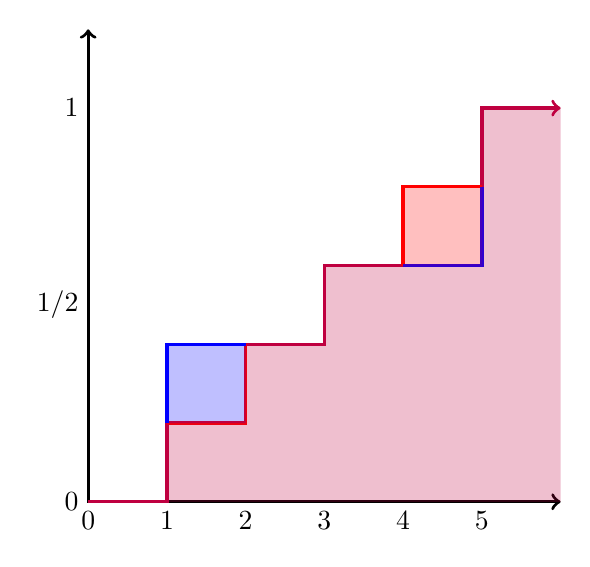
\begin{tikzpicture}
            \draw[very thick, <->] (0,6)--(0,0)--(6,0);
            
            \draw[very thick, purple] (0,0)--(1,0)--(1,1);
            \draw[very thick, purple] (2,2)--(3,2)--(3,3)--(4,3);
            \draw[very thick, purple,->] (5,4)--(5,5)--(6,5);
            
            \draw[very thick, red] (1,1)--(2,1)--(2,2);
            \draw[very thick, red] (4,3)--(4,4)--(5,4);


            \draw[very thick, blue] (1,1)--(1,2)--(2,2);
            \draw[very thick, blue] (4,3)--(5,3)--(5,4);

            \fill[purple, nearly transparent] (1,0)--(1,1)--(2,1)--(2,2)--(3,2)--(3,3)--(5,3)--(5,5)--(6,5)--(6,0)--(1,0);
            \fill[red, nearly transparent] (4,3)--(4,4)--(5,4)--(5,3)--(4,3);
            \fill[blue, nearly transparent] (1,1)--(2,1)--(2,2)--(1,2)--(1,1);

            \node[left] at (0,0) {0};
            \node[below] at (0,0) {0};
            \node[left] at (0,5) {1};
            \node[left] at (0,2.5) {1/2};

            \node[below] at (1,0) {1};
            \node[below] at (2,0) {2};
            \node[below] at (3,0) {3};
            \node[below] at (4,0) {4};
            \node[below] at (5,0) {5};   
        \end{tikzpicture}
        \caption{The cumulative distributions for \textcolor{blue}{\emph{p}} and \textcolor{red}{\emph{q}}. When the lines coincide, they are \textcolor{purple}{purple}.} Areas under both curves are lightly shaded in their color.
        \label{fig:4a}
    \end{figure}

     By inspection, neither gamble first-order stochastically dominates the other, as their CDFs cross. From Proposition 7, since the two gambles have the same mean, we can use the area under their CDFs to find out whether one second-order stochastically dominates the other. We will show that
    \[
    \int_{-\infty}^x G(y)dy \le \int_{-\infty}^x F(y)dy
    \]
    Since the distributions are discrete, we simply compare the values of the integral over distinct areas
    \[
    \begin{tabular}{|c|c|c|}
        \hline
        $x$ & $\int_{-\infty}^x G(y)dy$ & $\int_{-\infty}^x F(y)dy$ \\
        \hline
        $<1$ & 0 & 0 \\
        \hline
        $<2$ & 1/5 & 2/5\\
        \hline
        $<3$ & 3/5 & 4/5\\
        \hline
        $<4$ & 6/5& 7/5\\
        \hline
        $<5$ & 10/5& 10/5\\
        \hline
    \end{tabular}
    \]
    This extends to all other values of $y$ by inspection. Since $\int_{-\infty}^x G(y)dy \le \int_{-\infty}^x F(y)dy$ for all $y$, $G$ second-order stochastically dominates $F$, so the agent will prefer $p$ to $q$

    \item[(b)] No. We can see that, by comparing two different risk-averse expected utility functions, she may sometimes prefer one or the other. First, take the Bernoulli utility function $u(x) = \sqrt{x}$. The associated expected utility functions are
    \[
    U(p') = \frac{1}{5}\sqrt{1} + \frac{1}{5}\sqrt{2} + \frac{1}{5}\sqrt{3} + \frac{1}{5}\sqrt{4} + \frac{1}{5}\sqrt{5} \approx 1.68
    \]
    \[
    U(q') = \frac{2}{5}\sqrt{1} + \frac{1}{5}\sqrt{4} + \frac{2}{5}\sqrt{5} \approx 1.69
    \]
    So with the concave Bernoulli utility function $u(x) = \sqrt{x}$, the agent would prefer $q'$ to $p'$. However, with the Bernoulli utility function $u(x) = \ln x$, the expected utility functions are
    \[
    U(p') = \frac{1}{5}\ln{1} + \frac{1}{5}\ln{2} + \frac{1}{5}\ln{3} + \frac{1}{5}\ln{4} + \frac{1}{5}\ln{5} \approx 0.96
    \]
    \[
    U(q') = \frac{2}{5}\ln{1} + \frac{1}{5}\ln{4} + \frac{2}{5}\ln{5} \approx 0.92
    \]
    So with the concave Bernoulli utility function $u(x) = \ln{x}$, the agent would prefer $p'$ to $q'$. Thus, we cannot say unambiguously which one she would prefer.

    \item[(c)] To find how the decision maker will rank $p$ vs $q$, we simply find a measure for the expected utility in terms of $a$:
    \[
    U(p) = \frac{1}{5}(1 - a) +  \frac{1}{5}(2 - 4a) +  \frac{1}{5}(3 - 9a) +  \frac{1}{5}(4 - 16a) +  \frac{1}{5}(5 - 25a) = 3 - 11a
    \]
    \[
    U(q) = \frac{2}{5}(1-a) + \frac{1}{5}(3 - 9a) + \frac{2}{5}(5 - 25a) = 3 - \frac{61}{5}a < 3 - 11a
    \]
    Thus, the decision maker would prefer $p$ to $q$, because $\frac{61}{5} > 11$. One could also find this by noting that $u$ is strictly concave, so the decision-maker is risk-averse and so would unambiguously prefer $p$ from part (a).

    \medskip

    To find how the decision maker will rank $p'$ vs $q'$, we similarly find a measure for the expected utility in terms of $a$:
    \[
    U(p') = U(p) = 3 - 11a
    \]
    \[
    U(q') = \frac{2}{5}(1 - a) + \frac{1}{5}(4 - 16a) + \frac{2}{5}(5 - 25a) = \frac{16}{5} - \frac{68}{5}a
    \]
    Thus, when $a = 1/13$, $U(p') = U(q')$, so $p' \sim q'$. When $a < 1/13$, $U(q') > U(p')$, so $q' \succ p'$, and when $a > 1/13$, $U(p') > U(q')$, so $p' \succ q'$.
\end{itemize}

\paragraph{Problem 5:} Consider the portfolio problem discussed in class: there is an investor with wealth $w$, who has to choose how to allocate this wealth between a riskless asset that pays gross return $r$ for sure and a risky asset whose gross return as a cdf $F$. The investor has a ``well-behaved'' (differentiable, concave, increasing) utility function. This problem asks you to consider the effect on investment of a change in the distribution of the risky asset. 
\begin{itemize}
    \item[(a)] Suppose that the return on the risky asset improves so that its cdf if now $G$, where $G$ first-order stochastically dominates $F$. Construct a simple example (the simpler the better) where such a change could nevertheless lead the investor to decrease the amount he invests in the risky asset.

    \item[(b)] Show that if $G$ dominates $F$ in the likelihood ratio order, then the consumer will invest more in the risky asset if it has distribution $G$ than if it has distribution $F$. (Hint: try to mimic the proof in the lecture notes that less risk-averse consumers invest more in a given risky asset.)
\end{itemize}

\medskip
\textbf{Solutions:}

\begin{itemize}
    \item[(a)] Assume that the risky asset assumes value $a$ with probability $0.5$ and $0$ with probability $0.5$. If $G$ has value $a'$ and $F$ has value $a$, where $a' > a$, that is a first-order stochastic domination by inspection. Take as an example a consumer with Bernoulli utility function $u(x) = x - \frac{1}{2} x^2$. The consumer's maximization problem, where $x$ is the amount invested in the risky asset and $w$ is initial wealth, is
    \[
    \max_{x \in [0,w]} \frac{1}{2} u(r(w-x)) + \frac{1}{2}u(ax + r(w-x))
    \]
    Taking first-order conditions, we get
    \[
        -\frac{1}{2}r u'(r(w-x)) + \frac{1}{2}(a-r) u'(ax + r(w-x)) = 0
    \]
    Solving for $x$, noting that $u'(x) = 1-x$, we get
    \[
    x^* = \frac{1 - rw}{a-2r}
    \]
    Taking the derivative with respect to $a$, we get
    \[
    \frac{\partial x^*}{\partial a} = \frac{rw - 1}{(a-2r)^2}
    \]
    With some assumptions ($rw < 1$, $a>2r$), we get that this derivative is negative, meaning that the amount invested in the risky asset will go down, even if the new cdf first-order stochastically dominates the old.

    \item[(b)] 
    \begin{proof}
    Assume that the gross return of the risky asset is $\varepsilon$. Also denote $y = r(w-x)$. The consumer's maximization problem for cdf $F$ is
    \[
    \begin{array}{ll}
        \max_{x,y \ge 0} & \expect_F\left[ u(\varepsilon x + y)\right] \\
        \text{s.t.} & x + \frac{y}{r} = w
    \end{array}
    \]
    Call the objective function $V(x,y;F)$ (analogously, for cdf $G$ it is $V(x,y;G)$). The marginal rate of substitution between $x$ and $y$ is
    \[
    \frac{\partial V(x,y;F) / \partial x}{\partial V(x,y;F) / \partial y} = \frac{\expect_F\left[ \varepsilon u'(\varepsilon x + y)\right]}{\expect_F\left[ u'(\varepsilon x + y)\right]} = \int \varepsilon R(\varepsilon,x,y;F) d\varepsilon
    \]
    where
    \[
    R(\varepsilon,x,y;F) = \frac{u'(\varepsilon x + y)}{\expect_F\left[ u'(\varepsilon x + y)\right]} f(\varepsilon)
    \]
    where $f(\varepsilon)$ is the pdf of $\varepsilon$. We view $R(\cdot,x,y;F)$ as the pdf of some random variable, as $\int R(\varepsilon,x,y;F) d\varepsilon = 1$. Define $R(\cdot,x,y;G)$ analogously. To compare the consumer's choice under the two distributions, note that
    \[
    \frac{R(\varepsilon,x,y;G)}{R(\varepsilon,x,y;F)} = \frac{g(\varepsilon)}{f(\varepsilon)} \frac{\expect_F\left[ u'(\varepsilon x + y)\right]}{\expect_F\left[ u'(\varepsilon x + y)\right]}
    \]
    Since $G$ dominates $F$ in the likelihood ratio order, $\frac{g(\varepsilon)}{f(\varepsilon)}$ is nondecreasing in $\varepsilon$, which means that $\frac{R(\varepsilon,x,y;G)}{R(\varepsilon,x,y;F)}$ is nondecreasing in $\varepsilon$. This means that $R(\varepsilon,x,y;G)$ dominates $R(\varepsilon,x,y;F)$ in the likelihood ratio order, meaning that it first order stochastically dominates it. Thus, we have that
    \[
    \frac{\partial V(x,y;G) / \partial x}{\partial V(x,y;G) / \partial y} = \int \varepsilon R(\varepsilon,x,y;G) d\varepsilon \ge \int \varepsilon R(\varepsilon,x,y;F) d\varepsilon = \frac{\partial V(x,y;F) / \partial x}{\partial V(x,y;F) / \partial y}
    \]
    This means that $V(x,y;G)$ has the Spence-Mirrlees single-crossing property, meaning that the consumer will take more risk under $G$ than under $F$.
    \end{proof}
\end{itemize}



\newpage
\subsection{Uncertainty (Barseghyan)}

\subsubsection{Barseghyan Homework}

\paragraph{Problems.} MWG Chapter 6C. Problems 9, 14, 15, 16, 17, 18 and 19.

\begin{itemize}
	\item[9.] The purpose of this problem is to examine the implications of uncertainty and precaution in a simple consumption-savings decision problem.
	
	In a two-period economy, a consumer has first-period initial wealth $w$. The consumer's utility level is given by $u(c_1,c_2) = u(c_1) + v(c_2)$, where $u(\cdot)$ and $v(\cdot)$ are concave functions and $c_1$ and $c_2$ denote consumption levels in the first and second period respectively. Denote by $x$ the amount saved by the consumer in the first period (so that $c_1 = w-x$ and $c_2 = x$), and let $x_0$ be the optimal value of $x$ in this problem.
	
	We now introduce uncertainty in this economy. If the consumer saves an amount $x$ in the first period his wealth in the second period is given by $x + y$, where $y$ is distributed according to $F(\cdot)$. In what follows, $\expect[\cdot]$ always denotes expectation with respect to $F(\cdot)$. Assume that the Bernoulli utility function over realized wealth levels in the two periods $(w_1,w_2)$ is $u(w_1) + v(w_2)$. Hence, the consumer now solves
	\[
	\max_x u(w-x) + \expect[v(x+y)]
	\]
	Denote the solution to this problem by $x\opt$.
	\begin{itemize}
		\item[(a)] Show that if $\expect[v'(x_0+y)] > v'(x_0)$, then $x\opt > x_0$.
		\item[(b)] Define the \emph{coefficient of absolute prudence} of a utility function $v(\cdot)$ at wealth level $x$ to be $-v'''(x) / v''(x)$. Show that if the coefficient of absolute prudence of a utility function $v_1(\cdot)$ is not larger than the coefficient of absolute prudence of utility function $v_2(\cdot)$ for all levels of wealth, then $\expect[v_1'(x_0 + y)] > v_1'(x_0)$ implies $\expect[v_2'(x_0 + y)] > v_2'(x_0)$. What are the implications of this fact in the context of part (a)?
		\item[(c)] Show that if $v'''(\cdot) > 0$ and $\expect[y] = 0$, then $\expect[v'(x+y)] > v'(x)$ for all values of $x$.
		\item[(d)] Show that if the coefficient of absolute risk aversion of $v(\cdot)$ is decreasing in wealth, then $-v'''(x) / v''(x) > -v''(x) / v'(x)$ for all $x$, and hence $v'''(\cdot) > 0$.
	\end{itemize}
	\item[14.] Consider two risk-averse decision makers (i.e., two decision makers with concave Bernoulli utility functions) choosing among monetary lotteries. Define the utility function $u\opt(\cdot)$ to be strongly more risk-averse than $u(\cdot)$ if and only if there is a positive constant $k$ and a nonincreasing and concave function $v(\cdot)$ such that $u\opt(x) = ku(x) + v(x)$ for all $x$. The monetary amounts are restricted to lie in the interval $[0,r]$.
	\begin{itemize}
		\item[(a)] Show that if $u\opt(\cdot)$ is strongly more risk-averse than $u(\cdot)$, then $u\opt(\cdot)$ is more risk-averse than $u(\cdot)$ in the usual Arrow-Pratt sense.
		\item[(b)] Show that if $u(\cdot)$ is bounded, then there is no $u\opt(\cdot)$ other than $u\opt(\cdot) = ku(\cdot) + c$, where $c$ is a constant, that is strongly more risk-averse than $u(\cdot)$ on the entire interval $[0,\infty)$ . 
		\item[(c)] Using (b), argue that the concept of a strongly more risk-averse utility function is stronger (ie more restrictive) than the Arrow-Pratt concept of a more risk-averse utility function.
	\end{itemize}
	\item[15.] Assume that, in a world with uncertainty, there are two assets. The first is a riskless asset that pays 1 dollar. The second pays amounts $a$ and $b$ with probabilities $\pi$ and $1-\pi$, respectively. Denote the demand for the two assets by $(x_1,x_2)$. 
	
	Suppose that a decision maker's preferences satisfy the axioms of expected utility theory and that he is a risk averter. The decision maker's wealth is 1, and so are the prices of the assets. Therefore, the decision maker's budget constraint is given by
	\[
	x_1 + x_2 = 1, x_1,x_2 \in [0,1]
	\]
	\begin{itemize}
		\item[(a)] Give a simple \emph{necessary} condition, involving ($a$ and $b$ only) for the demand for the riskless asset to be strictly positive.
		\item[(b)] Give a simple \emph{necessary} condition, involving ($a$, $b$, and $\pi$ only) for the demand for the risky asset to be strictly positive.
	\end{itemize}
	In the next three parts, assume that the conditions obtained in (a) and (b) are satisfied.
	\begin{itemize}
		\item[(c)] Write down the first order conditions for utility maximization in this asset demand problem.
		\item[(d)] Assume that $a < 1$. Show by analyzing the first order conditions that $\partial x_1 / \partial a \le 0$. 
		\item[(e)] Which sign do you conjecture for $\partial x_1 / \partial \pi$? Give an economic interpretation.
		\item[(f)] Can you prove your conjecture in (e) by analyzing the first order conditions?
	\end{itemize}
	\item[16.] An individual has Bernoulli utility function $u(\cdot)$ and initial wealth $w$. Let lottery $L$ offer a payoff of $G$ with probability $p$ and a payoff of $B$ with probability $1-p$.
	\begin{itemize}
		\item[(a)] If the individual owns the lottery, what is the minimum price he would sell it for?
		\item[(b)] If he does not own it, what is the maximum price he would be willing to pay for it?
		\item[(c)] Are buying and selling prices equal? Give an economic interpretation for your answer. Find conditions on the parameters of the problem under which buying and selling prices are equal.
		\item[(d)] Let $G = 10$, $B = 5$, $w = 10$, and $u(x) = \sqrt{x}$. Compute the buying and selling prices for this lottery and this utility function.
	\end{itemize}
	\item[17.] Assume that an individual faces a two-period portfolio allocation problem. In period $t = 0,1$, his wealth $w_t$ is to be divided between a safe asset with return $R$ and a risky asset with return $x$. The initial wealth at period 0 is $w_0$. Wealth at period $t = 1,2$ depends on the portfolio $\alpha_{t-1}$ chosen at period $t-1$ and on the return $x_t$ realized in period $t$, according to
	\[
	w_t = ((1-\alpha_{t-1}R + \alpha_{t-1}x_t)w_{t-1}
	\]
	The objective of this individual is to maximize the expected utility of terminal wealth $w_2$. Assume that $x_1$ and $x_2$ are independently and identically distributed. Prove that the individual optimally sets $\alpha_0 = \alpha_1$ if his utility function exhibits constant relative risk aversion. Show that this fails to hold if his utility function exhibits constant absolute risk aversion.
	\item[18.] Suppose that an individual has a Bernoulli utility function $u(x) = \sqrt{x}$.
	\begin{itemize}
		\item[(a)] Calculate the Arrow-Pratt coefficients of absolute and relative risk aversion at the level of wealth $w = 5$.
		\item[(b)] Calculate the certainty equivalent and the probability premium for a gamble $(16,4;\frac{1}{2},\frac{1}{2})$.
		\item[(c)] Calculate the certainty equivalent and the probability premium for a gamble $(36,16;\frac{1}{2},\frac{1}{2})$. Compare this result with the one in (b) and interpret.
	\end{itemize}
	\item[19.] Suppose that an individual has a Bernoulli utility function $u(x) = -e^{-\alpha x}$ where $\alpha > 0$. His (nonstochastic) initial wealth is given by $w$. There is one riskless asset abd there are $N$ risky assets. The return per unit invested on the riskless asset is $r$. The returns of the risky assets are jointly normally distributed random variables with means $\mu = (\mu_1,\dots,\mu_N)$ and variance covariance matrix $V$. Assume that there is no redundancy in the risky assets, so that $V$ is of full rank. Derive the demand function for those $N+1$ assets.
\end{itemize}


\paragraph{Solutions.} (Gabe's solutions. Not graded, there may exist mistakes)

\begin{itemize}
	\item[9.] The consumer solves the problem
	\[
	\max_x u(w - x) + \expect[v(x+y)]
	\]
	where $y \sim F(\cdot)$. Denote the solution to this problem as $x\opt$ and the solution to the problem where $y$ is degenerate with mean 0 as $x_0$.
	\begin{itemize}
		\item[(a)] Recall that in the degenerate problem, since $u$ and $v$ are concave, we have that $v'(x_0) - u'(w-x_0) = 0$. If $\expect[v'(x_0 + y)] > v'(x_0)$, we have that $\expect[v'(x_0 + y)] - u'(w - x_0) > 0$, so $x_0$ is not a maximizer of the problem. It remains to show that the true maximizer is greater than $x_0$. At $x_0$, we have that $\expect[v'(x_0 + y)] > u'(w - x_0)$. At the true maximizer $x\opt$, we have that $\expect[v'(x\opt + y)] = u'(w - x\opt)$. Conclusion follows by noting that $u$ and $v$ are concave, so $u'$ and $v'$ are decreasing in the argument. Thus, $x\opt > x_0$.
		\item[(b)] We have that for $v_1$ and $v_2$, $-v_1'''(x)/v_1''(x) \le -v_2'''(x)/v_2''(x)$ for all $x$, and that $\expect[v_1'(x_0+y)] > v_1'(x_0)$. Note that the coefficient of absolute risk aversion of $v_i'$ is equivalent to the coefficient of absolute prudence of $v_i$. Thus, from Proposition 6.C.2 in Mas-Colell, we have that since $v'_1$ has a coefficient of absolute risk aversion that is not greater than $v'_2$, $v'_2$ has a greater certainty equivalent than $v'_1$, meaning that $\expect[v_2'(x_0 + y)] > v_2'(x_0)$. In the context of part (a), this implies that if one individual decides to invest in a risky lottery, a second individual with a not-greater coefficient of absolute prudence will also invest, and they will not invest less.
		\item[(c)] We have that $v'''(x) > 0$ for all $x$, then $v'$ is convex, meaning that $v'$ exhibits risk-loving behavior. Since $\expect[y] = 0$, we have that $\expect[v'(x + y)] > v'(x)$ for all $x$.
		\item[(d)] We have that the coefficient of absolute risk aversion is decreasing in wealth, meaning that
		\[
		\frac{\partial}{\partial w} \barl -\frac{v''(x)}{v'(x)}\barr < 0 \Longrightarrow -\frac{v'''(x)v'(x) - (v''(x))^2}{(v'(x))^2} = \frac{v''(x)}{v'(x)} \parl \frac{v''(x)}{v'(x)} - \frac{v'''(x)}{v''(x)} \parr < 0
		\]
		Thus, we have that $-\frac{v''(x)}{v'(x)} < - \frac{v'''(x)}{v''(x)}$.
	\end{itemize}
	\item[14.] We have that $u\opt(\cdot)$ is strongly more risk-averse than $u(\cdot)$ if and only if there exists a positive constant $k$ and a nonincreasing, concave function $v(\cdot)$ such that $u\opt(x) = ku(x) + v(x)$ for all $x$.
	\begin{itemize}
		\item[(a)] We have that the coefficient of absolute risk aversion for $u\opt$ at some $x$ is
		\[
		r(x,u\opt) = - \frac{ku''(x) + v''(x)}{ku'(x) + v'(x)}
		\] 
		we want to show that
		\[
		- \frac{ku''(x) + v''(x)}{ku'(x) + v'(x)} \ge -\frac{u''(x)}{u'(x)} \Longrightarrow u'(x)(ku''(x)+v''(x)) \le u''(x)(ku'(x) + v'(x))
		\]
		This simplifies to
		\[
		ku'(x)u''(x) + u'(x)v''(x) \le ku'(x)u''(x) + u''(x)v'(x) \Longrightarrow  u'(x)v''(x) \le u''(x)v'(x)
		\]
		Which holds as long as
		\[
		-\frac{v''(x)}{v'(x)} \ge -\frac{u''(x)}{u'(x)}
		\]
		Since, by assumption, $u$ is increasing and concave, and $v$ is non-increasing and concave, the left side is non-negative and the right side is non-positive. Conclusion follows.
		
		\item[(b)] Suppose FSOC that there exists $u\opt(x) = ku(x) + v(x)$, where $v$ is non-constant, non-increasing, and concave. Define $M$ such that $M = \inf \{C \in \reals : u(x) \le C \forall x\}$. Since $u$ is increasing, as $x \to \infty$, $u(x) \to M$. However, since $v$ is non-constant and non-increasing, $\exists x \in \reals$ sufficiently large such that $u\opt(x) > u\opt(x + \varepsilon)$ for some $\varepsilon > 0$. This contradicts the assumption that $u\opt$ must be increasing.
		
		\item[(c)] We have from (a) that strong risk aversion implies Arrow-Pratt risk aversion. It remains to show that the converse is not true. Consider the functions $u(x) = -\exp(-\alpha x)$ and $v(x) = -\exp(-\beta x)$, where $\beta > \alpha$. Both functions exhibit constant absolute risk aversion, so $v$ is more risk-averse than $u$ in the Arrow-Pratt sense. However, since they are each bounded above, by (b) $v$ is not strongly more risk-averse than $u$.
	\end{itemize}
	\item[15.] We have a risk-averse decision maker, investing $x_1$ in a riskless asset and $x_2$ in a risky asset that pays $a$ with probability $\pi$ and $b$ with probability $1-\pi$. They begin with $w = 1$. 
	\begin{itemize}
		\item[(a)] Since the decision-maker is risk-averse, they will invest strictly positive levels in the riskless asset if there is a probability of loss with respect to the risky asset. Thus, the necessary condition is that at least one of $a,b$ is strictly less than 1.
		\item[(b)] Again, since the decision-maker is risk-averse, they will invest in the risky asset only if its expected value is greater than that of the riskless asset, \ie when $\pi a + (1-\pi)b > 1$. 
		\item[(c)] The decision-maker is maximizing the problem
		\[
		\max_{x_1,x_2} \pi u(x_1 + ax_2) + (1-\pi)u(x_1 + bx_2) \st x_1,x_2 \in [0,1], x_1 + x_2 = 1
		\]
		The first condition falls away because we're assuming that the conditions from (a) and (b) hold, so the Lagrangian this admits is
		\[
		\mathcal{L} = \pi u(x_1 + ax_2) + (1-\pi)u(x_1 + bx_2) + \lambda(1 - x_1 - x_2)
		\]
		The first order conditions are
		\[
		\frac{\partial \mathcal{L}}{\partial x_1} = \pi u'(x_1 + ax_2) + (1-\pi)u'(x_1 + bx_2) - \lambda = 0
		\]
		\[
		\frac{\partial \mathcal{L}}{\partial x_2} = a\pi u'(x_1 + ax_2) + b(1-\pi)u'(x_1 + bx_2) - \lambda = 0
		\]
		which, combining, get
		\[
		\pi u'(x_1 + ax_2) + (1-\pi)u'(x_1 + bx_2) = a\pi u'(x_1 + ax_2) + b(1-\pi)u'(x_1 + bx_2) 
		\]
		which imply
		\[
		\pi(1-a) u'(x_1 + ax_2) + (1-\pi)(1-b)u'(x_1 + bx_2) = 0
		\]
		The final first order condition is
		\[
		\frac{\partial \mathcal{L}}{\partial \lambda} = 1 - x_1 -x_2  = 0 \Longrightarrow x_1 + x_2 = 1
		\]
		\item[(d)] Using the implicit function theorem, and holding $b$ constant, define 
		\[
		g(x_1,a,\pi) = \pi(1-a) u'(x_1 + a(1-x_1)) + (1-\pi)(1-b)u'(x_1 + b(1-x_1))
		\]
		We have that
		\[
		\frac{\partial x_1}{\partial a} = -\frac{\frac{\partial g}{\partial a }}{\frac{\partial g}{\partial x_1}} = -\frac{-\pi u'(x_1 + a(1-x_1)) + \pi(1-a)(1-x_1)u''(x_1 +a(1-x_1))}{\pi(1-a)(1-a) u''(x_1+a(1-x_1)) + (1-\pi)(1-b)(1-b)u''(x_1 + b(1-x_1))}
		\]
		where all terms in the numerator and denominator are negative, so $\frac{\partial x_1}{\partial a} \le 0$.
		\item[(e)] If we are assuming, like in (d), that $a < 1$, it follows that $b > 1$. Thus, as $\pi$ increases, the lottery gets worse, so the decision maker would invest more in the riskless asset. Thus, I conjecture that $\frac{\partial x_1}{\partial \pi} > 0$.
		\item[(f)] From the first order conditions and the implicit function theorem, we have that
		\[
		\frac{\partial x_1}{\partial \pi} = -\frac{\partial g / \partial \pi}{\partial g / \partial x_1}
		\]
		We know that the denominator is negative, from part (d). It remains to show that the numerator is positive, and conclusion will follow. We have that
		\[
		\frac{\partial g}{\partial \pi} = \underbrace{(1-a)u'(x_1 + a(1-x_1))}_{> 0} - \underbrace{(1-b)u'(x_1 + b(1-x_1))}_{<0} > 0
		\]
	\end{itemize}
	\item[16.] An individual has Bernoulli utility function $u(\cdot)$ and initial wealth $w$. Let lottery $L$ offer a payoff of $G$ with probability $p$ and a payoff of $B$ with probability $(1-p)$.
	\begin{itemize}
		\item[(a)] The individual would sell the lottery for no less than the amount that would guarantee the same expected utility -- \ie, a price $y$ such that
		\[
		p u(w + G) + (1-p)u(w + B) = u(w + y)
		\]
		\item[(b)] They would purchase the lottery for an amount $x$ such that they would have the same expected utility whether they had the lottery or not -- \ie, a price $x$ such that
		\[
		p u(w - x + G) + (1-p)u(w - x+B) = u(w)
		\]
		\item[(c)] In general, $x \ne y$, as the different levels of wealth will change how much the lottery is `worth' to the decision maker. However, if $u$ exhibits constant absolute risk aversion, then they will coincide. If $u$ exhibits CARA, then the above conditions imply that
		\[
		w - c_w = (w-x) - c_{w - x}
		\]
		where $c_w$ is the certainty equivalent of the lottery with wealth $w$ and $c_{w-x}$ is the certainty equivalent of the lottery with wealth $w-x$.
		\item[(d)] Directly calculating (using Wolfram), we get that $y$ solves
		\[
		p \sqrt{20} + (1-p)\sqrt{15} = \sqrt{10 + y} \Longrightarrow y = -5\parl 4\sqrt{3} p^2 - 7p^2 - 4\sqrt{3}p + 6p - 1\parr
		\]
		and $x$ solves
		\[
		p \sqrt{20 - x} + (1-p)\sqrt{15 - x} = \sqrt{10} \Longrightarrow x = \frac{5\parl 2p^3 + 7p^2 \pm 2\sqrt{2}\sqrt{-2p^5 + 7p^4 - 8p^3 + 3p^2} - 8p+1\parr}{4p^2-4p+1}
		\]
	\end{itemize}
	\item[17.] We have that an individual faces a two-period portfolio allocation problem, dividing her wealth between a risky asset with return $x$ and a safe asset with return $R$. They have initial wealth $w_0$, and in period $t \in \{1,2\}$ their wealth depends on the portfolio $\alpha_{t-1}$ chosen previously, defined by
	\[
	w_t = ((1-\alpha_{t-1})R + \alpha_{t-1}x_t)w_{t-1}
	\]
	The individual is maximizing $w_2$, where we assume that $x_1,x_2$ are i.i.d. 
	
	\begin{proof}
		First, assume that $u$ has CRRA preferences. The wealth at the end of each period is 
		\[
		w_1 = ((1-\alpha_{0})R + \alpha_{0}x_1)w_{0} \quad \text{ and }\quad w_2 = ((1-\alpha_{1})R + \alpha_{1}x_2)w_{1}
		\]
		Combining, we get that
		\[
		w_2 = ((1-\alpha_{1})R + \alpha_{1}x_2)((1-\alpha_{0})R + \alpha_{0}x_1)w_{0}
		\]
		Since CRRA preferences are scale-invariant, for any $\lambda$ we have that $u(\lambda x) = \lambda^{1-\sigma} u(x)$, where $\sigma$ is the coefficient of relative risk aversion. When the consumer is maximizing the expected utility, we have that
		\[
		\expect[u(w_2)] = \expect\barl ((1-\alpha_{1})R + \alpha_{1}x_2)^{1-\sigma} u(w_1)\barr = \expect[u(w_1)] \cdot ((1-\alpha_{1})R + \alpha_{1}\expect[x_2])^{1-\sigma}
		\]
		Thus, the choice of $\alpha$ that maximizes $w_1$ will also maximize $w_2$, since $x_i$ are i.i.d., and $\alpha_0 = \alpha_1$.
		
		Next, assume that $u$ has CARA preferences. We know that $u$ has the form $u(x) = -\exp(-\gamma x)$, where $\gamma > 0$ is the coefficient of absolute risk aversion. Thus, 
		\[
		\expect[u(w_2)] = \expect\barl  u(w_1)\exp(-\gamma(((1-\alpha_{1})R + \alpha_{1}x_2))) \barr
		\]
		However, we cannot split the expectation here as above, since we do not know that the relevant moments for $x$ necessarily exist. Thus, the choice of $\alpha_1$ depends on $x_1$, so it will not necessarily hold that $\alpha_0 = \alpha_1$.
	\end{proof} 
	\item[18.] Suppose that a decision maker has utility $u(x) = \sqrt{x}$.
	\begin{itemize}
		\item[(a)] We have that wealth $w = 5$. The coefficient of absolute risk aversion is
		\[
		-\frac{u''(w)}{u'(w)} = -\frac{(-0.25)w^{-1.5}}{(0.5)w^{-0.5}} = \frac{1}{2} \frac{\sqrt{5}}{\sqrt{125}} = \frac{1}{2	}\cdot \frac{1}{5} = 0.1
		\]
		The coefficient of relative risk aversion is
		\[
		-w \frac{u''(w)}{u'(w)} = 5 \cdot \frac{1}{10} = 0.5
		\]
		\item[(b)] The certainty equivalent of this lottery is
		\[
		u^{-1}(0.5 u(16) + 0.5u(4)) = u^{-1}(2 + 1) = u^{-1}(3) = 9
		\]
		The probability premium is $\pi$ such that
		\[
		u(10) = (0.5 + \pi)u(16) + (0.5 - \pi)u(4) \Longrightarrow \sqrt{10} = 2 + 4\pi + 1 - 2\pi \Longrightarrow \pi = \frac{\sqrt{10}-3}{2}
		\]
		\item[(c)] The certainty equivalent of this lottery is
		\[
		u^{-1}(0.5 u(36) + 0.5u(16)) = u^{-1}(3 + 2) = u^{-1}(5) = 25
		\]
		The probability premium is $\pi$ such that
		\[
		u(26) = (0.5 + \pi)u(36) + (0.5 - \pi)u(16) \Rightarrow \sqrt{26} = 3 + 6\pi + 2 - 4\pi \Rightarrow \pi = \frac{\sqrt{26}-5}{2}
		\]
		The probability premium is higher in the first lottery, which implies that $u$ has decreasing absolute risk aversion, implied by the fact that it has constant relative risk aversion.
	\end{itemize}
	\item[19.] We have that an individual has utility $u(x) = -\exp(-\alpha x)$ with $\alpha > 0$, and initial wealth $w$. He invests in a riskless asset with return $r$ and $N$ jointly normally distributed random assets with means $\mu = (\mu_1,\dots,\mu_N)$ and variance $V$. We assume that $V$ is full rank.
	
	Denote by $x_i$ the amount invested in risky asset $i$, and by $y_i$ its return. The agent's realized wealth is
	\[
	w' = \parl w - \sum_{i=1}^N x_i\parr r + \sum_{i=1}^N x_i y_i
	\]
	By the properties of jointly normal distributions, $w' \sim \normal\parl \parl w - \sum_{i=1}^N x_i\parr r + \sum_{i=1}^N x_i \mu_i, x^{T} V x\parr$. The expected utility of this is
	\[
	\expect[u(w')] = \expect[-\exp(-\alpha w')]
	\]
	Using the properties of the moment generating function of a normal random variable, we have that
	\[
	\expect[u(w')] = -\exp\barl\parl \parl w - \sum_{i=1}^N x_i\parr r + \sum_{i=1}^N x_i \mu_i\parr(-\alpha) - (x^T Vx) \frac{\alpha^2}{2}\barr
	\]
	Monotonically transforming this by $\ln(\cdot)$, we get that expected utility is maximized when
	\[
	-\alpha (\mu - r) - \alpha^2 Vx = 0 \Longrightarrow x = \frac{\mu - r}{\alpha V}
	\]
	where the $-$ in the numerator denotes elementwise subtraction.
\end{itemize}
\subsubsection{Outside Questions}

See the outside questions in Section 7.4.3, on the same topics. We also had two questions for a quiz in TA section, which I include here:

\begin{enumerate}
	\item An investor with initial wealth $\omega$ can invest only in the two following assets: a risk-free asset with return $R$, and a risky asset with return $x$, drawn from a distribution $F(\cdot)$ with positive support. The average return on this asset is higher than $R$. For emphasis, storage is not available. Suppose the investor has CARA preferences, with the preference parameter $\gamma$. Prove that the fraction of investment allocated to the risky asset (call it $\alpha$) is inversely proportional both to $\gamma$ and to $\omega$.
	\item Now suppose the investor has CRRA preferences, with the preference parameter $\sigma > 0$, $\sigma \ne 1$. Prove that the fraction of investment allocated to the risky asset (call it $\alpha$) is independent of $\omega$.
	\item A risk-averse agent possesses a productive asset (tree, factory, etc...) that generates a risky return distributed according to some $F(\cdot)$ with mean $R$.
	\begin{enumerate}
		\item If such assets are tradable and there is a continuum of perfectly competitive risk-neutral agents (bankers) in the market, what would you expect the price of the productive asset to be?
		\item Suppose now the economy consists of a continuum of risk-averse agents each possessing one productive asset. These assets generate returns distributed i.i.d. according to some $F(\cdot)$ with mean $R$. Assuming perfect competition and that all assets are tradable, what is the risk-free return in this economy?
		\item How much risk does each agent face?
	\end{enumerate}
\end{enumerate}

\newpage
\subsection{Information (Battaglini)}

\subsubsection{Battaglini Homework}

\begin{enumerate}
	\item A monopolist can produce goods in different qualities. The cost of producing a good of quality $s$ is $5s^2$. Consumers with type $\theta$ buy at most one unit and have utility function
	\[
	u(s \mid \theta) = \begin{cases} \theta \cdot s & \text{if the consume one unit of quality $s$} \\ 0 & \text{if they do not consume} \end{cases}
	\]
	The monopolist decides on the quality (or qualities) $s$ it is going to produce and price $T$. Consumers observe qualities and prices and decide which quality to buy if at all.
	\begin{enumerate}
		\item Characterize the first-best solution
		\item Suppose that the seller cannot observe $\theta$, and suppose that 
		\[
		\theta = \begin{cases} \theta_H & \text{with probability } 1-\beta \\ \theta_L & \text{with probability } \beta \end{cases}
		\]
		with $\theta_H > \theta_L > 0$. Characterize the second-best solution and consumers’ informational rents.
	\end{enumerate}
	\item Consider a government contracts with a monopolist to construct a bridge. The government is interested in choosing a contract that minimize the cost of such construction. The overall cost is $c = \theta - e$, which is observable to both the government and the monopolist. $\theta$ is the type of the monopolist; with probability $\beta$ the monopolist is an efficient type for $\theta = 5$, and with probability $1-\beta$ the monopolist is an inefficient type for $\theta = 8$. The monopolist can exert effort to reduce costs by paying private cost $\frac{e^2}{2}$. The government pays the monopolist $t + c$ where $t$ is a transfer. The monopolist has reservation utility at $\bar{u}$. 
	\begin{enumerate}
		\item Suppose the government could observe both the type $\theta$ and the effort $e$ of the monopolist. Characterize the first best effort $e^{FB}$ and transfer $t^{FB}$. 
		\item From now on, assume that the government cannot observe the type $\theta$ and effort $e$ of the monopolist. Write down the optimal contract which minimizes the cost, and is incentive compatible and individually rational.
		\item Characterize the second-best effort $e^{SB}$ and transfer $t^{SB}$ under such contract. Show each step clearly. Are first best effort $e^{FB}$ implementable for both types?
	\end{enumerate}
	\item (MWG 13.C.5) Assume a single firm and a single consumer. The firm's product may be of either high or low quality and is of high quality with probability $\lambda$. The consumer cannot observe quality before purchase and is risk neutral. The consumer's valuation of a high-quality product is $v_H$; her valuation of a low-quality product is $v_L$. The costs of production for high ($H$) and low ($L$) are $c_H$ and $c_L$ respectively. The consumer desires at most one unit of the product. Finally, the firm's price is regulated and set at $p$. Assume that $v_H > p > v_L > c_H > c_L$.
	\begin{enumerate}
		\item Given $p$, under what conditions will the consumer buy the product?
		\item Suppose that before the consumer decides to buy, the firm (which knows its type) can advertise. Advertising conveys no information directly, but consumers can observe the total amount of money the firm is spending on advertising, denoted by $A$. Can there be a separating perfect Bayesian equilibrium, that is, an equilibrium where the consumer rationally expects firms with different quality levels to pick different levels of advertising?
	\end{enumerate}
	\item (MWG 13.C.6) Consider the market for loans to finance investment projects. All investment projects require an outlay of 1 dollar. There are two types of projects: good and bad. A good project has a probability $p_G$ of yielding profits of $\Pi > 0$ and a probability $(1-p_G)$ of yielding profits of zero. For a bad project, the relative probabilities are $p_B$ and $(1-p_B)$ respectively, where $p_G > p_B$. The fraction of projects that are good is $\lambda \in (0,1)$. 
	
	Entrepreneurs go to banks to borrow cash to make the initial outlay (assume for now they borrow the entire amount). A loan contract specifies an amount $R$ that is supposed to be repaid to the bank. Entrepreneurs know the type of project they have, but the banks do not. In an event that a project yields profits of zero, the entrepreneur defaults on her loan and the bank receives nothing. Banks are competitive and risk-neutral. The risk-free rate of interest (the rate the banks pay to borrow funds) is $r$. Assume that
	\[
	p_G \Pi - (1 + r) > 0 > p_B \Pi - (1 + r)
	\]
	\begin{enumerate}
		\item Find the equilibrium level of $R$ and the set of projects financed. How does this depend on $p_G,p_B,\lambda,\Pi,$ and $r$?
		\item Now suppose that the entrepreneur can offer to contribute some fraction $x$ of the 1 dollar initial outlay from her own funds ($x \in [0,1]$). The entrepreneur is liquidity constrained, however, so that the effective cost of doing so is $(1 + \rho)x$, where $\rho > r$.
		\begin{enumerate}
			\item What is the entrepreneur's payoff as a function of her project type, her loan-repayment amount $R$, and her contribution $x$?
			\item Describe the best (from a welfare perspective) separating perfect Bayesian equilibrium of a game in which the entrepreneur first makes an offer of the amount of $x$ she is willing to put into a project, banks then respond by making offers specifying the level of $R$ they would require, and finally the entrepreneur accepts a bank's offer or decides not to go forward with the project. How does the amount contributed by entrepreneurs with good projects change with small changes in $p_B,p_G,\lambda,\Pi$, and $r$?
			\item How do the two types of entrepreneurs do in the separating equilibrium of (b)(ii) compared with the equilibrium in (a)?
		\end{enumerate}
	\end{enumerate}
\end{enumerate}


\paragraph{Solutions.} (Gabe's solutions, not graded, not including Problem 2 (b) and (c), which we did not learn)

\begin{enumerate}
	\item Monopolists and quality
	\begin{enumerate}
		\item In this case, where there is full information, the monopolist can choose a different quality level for each consumer type $\theta$, and maximize profit for that consumer type. Fix some $\theta > 0$. The consumer's utility from purchasing a good of quality $s$ at price $T$ is
		\[
		u(s,T ; \theta) = s \cdot \theta - T
		\]
		and the monopolist's profit is
		\[
		\pi_\theta(s,T) = T - 5s^2
		\]
		Note that if we were being precise here, these would be defined piecewise, if the consumer purchases the good or not. This is not necessary now, as we will show that the consumer $\theta$ will always purchase the good. The monopolist will ensure this by ensuring that $s \cdot \theta - T \ge 0$. In fact, to maximize profit, we will have that $s \cdot \theta - T = 0 \Longrightarrow T = s \cdot \theta$. This implies that profit is
		\[
		\pi_\theta(s,T) = s\cdot\theta - 5s^2
		\]
		Taking first order conditions, we get that the optimal quality is where
		\[
		\theta - 10s = 0 \Longrightarrow s\opt = \frac{\theta}{10}
		\]
		Substituting back, we get that the optimal price is
		\[
		T\opt = \theta \cdot  \frac{\theta}{10} = \frac{\theta^2}{10}
		\]
		The monopolist will extract all of the surplus of each consumer, so $u(s\opt,T\opt;\theta) = 0$ for all $\theta$, and for a certain $\theta$, 
		\[
		\pi_\theta(s\opt,t\opt) = T\opt - 5(s\opt)^2 = \frac{\theta^2}{10} - \frac{\theta^2}{20} = \frac{\theta^2}{20}
		\]
		\item Now, we suppose that the seller cannot observe $\theta$. We will assume that they produce goods of two qualities, $s_H$ and $s_L$, designated for each type of $\theta$, and priced at $T_H$, $T_L$. We will need the classic two constraints to hold: individual rationality and incentive compatibility. First, for the choice of each type of consumer to purchase to be rational, we need that
		\[
		\theta_Ls_L - T_L \ge 0 \qquad \text{ and } \qquad \theta_H s_H - T_H \ge 0
		\]
		Next, for the consumers to want their designated good rather than the other's, we need that
		\[
		\theta_Ls_L - T_L \ge \theta_L s_H - T_H \qquad \text{ and } \qquad \theta_Hs_H - T_H \ge \theta_H s_L - T_L
		\]
		The monopolist maximizes profit subject to these constraints, where expected profit is
		\[
		\Pi = \beta (T_L - 5s_L^2) + (1-\beta)(T_H - 5s_H^2)
		\]
		We will make the standard assumptions that the individual rationality constraint for the low type and the incentive compatibility constraint for the high type each hold with equality. This implies that
		\[
		T_L = \theta_Ls_L \quad \text{ and } \quad T_H = \theta_H(s_H - s_L) + \theta_Ls_L
		\]
		Substituting, the monopolist's profit becomes
		\[
		\Pi = \beta(\theta_Ls_L - 5s_L^2) + (1-\beta)(\theta_H(s_H - s_L) + \theta_Ls_L - 5s_H^2)
		\]
		To find the optimal choice of $s_L$ and $s_H$, we take first order conditions, and get that
		\[
		\frac{\partial \Pi}{\partial s_L} = \beta (\theta_L - 10s_L) + (1-\beta)(\theta_L - \theta_H) = 0 \Longrightarrow s_L\opt = \frac{\theta_L - (1-\beta)\theta_H}{10\beta}
		\]
		and
		\[
		\frac{\partial \Pi}{\partial s_H} = (1-\beta)\theta_H - (1-\beta)10s_H = 0 \Longrightarrow s_H\opt = \frac{\theta_H}{10}
		\]
		From the binding constraints, we can calculate the optimal prices. We have that
		\[
		T_L\opt = \theta_L \cdot \frac{\theta_L - (1-\beta)\theta_H}{10\beta} = \frac{\theta_L^2 - (1-\beta)\theta_H\theta_L}{10\beta}
		\]
		and
		\[
		T_H\opt = \theta_H \parl \frac{\theta_H}{10} - \frac{\theta_L - (1-\beta)\theta_H}{10\beta}\parr + \frac{\theta_L^2 - (1-\beta)\theta_H\theta_L}{10\beta} = \frac{\theta_H^2 - (2-\beta)\theta_H\theta_L + \theta_L^2}{10\beta}
		\]
		Note that these solutions admit a corner. We have that the fully described solution is:
		\begin{align*}
		s_L\opt &= \begin{cases} \frac{\theta_L - (1-\beta)\theta_H}{10\beta} &\theta_L \ge (1-\beta)\theta_H \\ 0 & \text{otherwise} \end{cases} \\
		s_H\opt &= \begin{cases} \frac{\theta_H}{10} & \theta_H^2 + \theta_L^2 \ge (2-\beta)\theta_H\theta_L \\ 0 & \text{otherwise} \end{cases} \\
		T_L\opt &= \begin{cases} \frac{\theta_L^2 - (1-\beta)\theta_H\theta_L}{10\beta} &  \theta_L \ge (1-\beta)\theta_H \\ 0 & \text{otherwise}\end{cases} \\
		T_H\opt &= \begin{cases} \frac{\theta_H^2 - (2-\beta)\theta_H\theta_L + \theta_L^2}{10\beta}& \theta_H^2 + \theta_L^2 \ge (2-\beta)\theta_H\theta_L \\ 0 & \text{otherwise} \end{cases}
		\end{align*}
		The informational rents are as follows. Since the low types' individual rationality constraint binds, they will attain no utility in equilibrium, which is the same as in the full information case. The high types, meanwhile, will (when we are not in the corner) attain utility:
		\[
		u(s\opt_H \mid \theta_H) = \theta_H \cdot s\opt_H - T\opt_H = \frac{\theta_H^2}{10} - \frac{\theta_H^2 - (2-\beta)\theta_H\theta_L + \theta_L^2}{10\beta} = \frac{\theta_L^2 - (1-\beta)\theta_H^2 - (2-\beta)\theta_L\theta_H}{10\beta}
		\]
		This is the informational rent the monopolist pays.
	\end{enumerate}
	\item Constructing a bridge
	\begin{enumerate}
		\item The government is attempting to minimize the cost, subject to the monopolist attaining their reservation utility. They will ensure that the monopolist's utility is exactly equal to their reservation, which functions as in individual rationality constraint. We need that
		\[
		\bar{u} = t  - \frac{e^2}{2} = t  - \frac{e^2}{2} \Longrightarrow t = \bar{u} + \frac{e^2}{2}
		\]
		The government is minimizing the total cost, which is the cost function $t + c$, subject to the constraint. Recalling that $c = \theta - e$, we get that they minimize
		\[
		C = \bar{u} + \frac{e^2}{2} + \theta - e
		\]
		Taking first order conditions to find the ideal induced effort, we get that
		\[
		\frac{\partial C}{\partial e} = e - 1 = 0 \Longrightarrow e^{FB} = 1
		\]
		The transfer that induces $e^{FB}$ is $t^{FB} = \bar{u} + \frac{1}{2}$. Note that the costs are different for each type. We have that $C^{FB}(5) = \bar{u} + 4.5$, and $C^{FB}(8) = \bar{u} + 7.5$.
		\item (Not able to figure out)
	\end{enumerate}
	\item MWG 13.C.5
	\begin{enumerate}
		\item Since the consumer is risk-neutral, they will buy the product if and only if its expected valuation is greater than its price. Mathematically, they will buy if and only if
		\[
		p \le \lambda v_H + (1-\lambda)v_L
		\]
		\item There can be no separating equilibrium. To see why, assume that we do have a separating equilibrium, in which high-quality firms spend $A$ on advertising and low-quality firms spend 0. Low-quality firms will spend 0 because in a separating equilibrium they will be immediately identified, so it is better to spend nothing than to advertise at all, since because $p > v_L$, nobody will buy their product. For incentive compatibility to hold for the high quality firms, it must be the case that $p - c_H - A > 0$. However, since $c_L < c_H$, in this case it would improve a low-quality firm's outcomes to deviate and spend $A$ pretending to be a high-quality firm, since $p - c_L - A > p - c_H - A > 0$. Thus, there will be deviation, so this is not a separating equilibrium.
	\end{enumerate}
	\item MWG 13.C.6
	\begin{enumerate}
		\item Note first that since banks are risk-neutral and competitive, the equilibrium level of $R$ will be the actuarily fair level of $R$. The expected payout to the bank for a funded project will be equal to $(1+r)$, the cost to fund a project. For an arbitrary project, funded at rate $R$, the expected payout means that
		\[
		\lambda \parl p_G R + (1-p_G)0\parr + (1-\lambda)\parl p_B R + (1-p_B)0\parr = 1+r
		\]
		which implies that
		\[
		\lambda p_G R + (1-\lambda)p_BR = 1 + r \Longrightarrow R = \frac{1+r}{\lambda p_G + (1-\lambda)p_B}
		\]
		A good entrepreneur will pursue a project if
		\[
		p_G(\Pi - R) \ge 0 \Longrightarrow \Pi \ge \frac{1+r}{\lambda p_G + (1-\lambda)p_B}
		\]
		and a bad entrepreneur will pursue a project if
		\[
		p_B(\Pi - R) \ge 0 \Longrightarrow \Pi \ge \frac{1+r}{\lambda p_G + (1-\lambda)p_B}
		\]
		Thus, if $R$ is low enough (meaning if the proportion of good projects is high enough), every entrepreneur's project will be both funded and pursued. If not, nobody's project will go forward.
		\item Suppose that the entrepreneur can contribute some of their own funds.
		\begin{enumerate}
			\item A good entrepreneur's expected payout is
			\[
			p_G (\Pi - (1-x)R) + (1-p_G)0 - x(1+\rho) = p_G(\Pi - R)+ x(p_GR - (1+\rho))
			\]
			A bad entrepreneur's expected payout is
			\[
			p_B (\Pi - (1-x)R) + (1-p_B)0 - x(1+\rho) = p_B(\Pi - R)+ x(p_BR - (1+\rho))
			\]
			\item Note first that since the rate that entrepreneurs borrow money is higher than banks, the best separating Bayesian equilibrium will be the one with the minimal $x$ that separates the good and bad entrepreneurs. In a separating equilibrium, banks will offer good entrepreneurs the actuarily fair rate $R = \frac{1+r}{p_G} < \Pi$, and will offer bad entrepreneurs the actuarily fair rate $R = \frac{1+r}{p_B} > \Pi$. In this equilibrium, no bad entrepreneurs will accept this rate. We can find $x$ by identifying the level above which a bad entrepreneur will attain negative utility if offered the good entrepreneurs' rate (rather than 0 from offering $x = 0$ and not pursuing the project). This will be the case if
			\[
			p_B\parl \Pi - \frac{1+r}{p_G}\parr + x\parl p_B \frac{1+r}{p_G} - (1+\rho)\parr = 0
			\]
			This implies that
			\[
			x\opt = \frac{p_B \Pi - p_B \frac{1+r}{p_G}}{(1+\rho) -  p_B \frac{1+r}{p_G}} = \frac{p_Gp_B\Pi - p_B(1+r)}{p_G(1+\rho) - p_B(1+r)}
			\]
			which is less than 1 since $p_B\Pi < 1+r < 1 + \rho$. Thus, our perfect separating Bayesian equilibrium is:
			
			Bad entrepreneurs will contribute $x = 0$ and accept the bank's offer if $R \le \Pi$. Good entrepreneurs will contribute $x = \frac{p_Gp_B\Pi - p_B(1+r)}{p_G(1+\rho) - p_B(1+r)} = x\opt$ and accept the bank's offer if $R \le \frac{1+r}{p_G}$. The bank will offer $R = \frac{1+r}{p_B}$ if the entrepreneur contributes 0 and $R = \frac{1+r}{p_G}$ if the entrepreneur contributes $x\opt$. All good projects will be funded, all bad projects will be abandoned.
			\item Bad entrepreneurs will be (weakly) worse off in the separating equilibrium, since they were sometimes funded previously (depending on $\lambda$) and are never funded now. Good entrepreneurs will be better off for small $\lambda$, since they now get funded, but worse off for large $\lambda$ since contributing their own funds is costly.
		\end{enumerate}
	\end{enumerate}
\end{enumerate}





\section{TA Sections}

TA Sections written by Feiyu Wang and Yuxuan Ma. Solutions written by Omar And\'{u}jar.

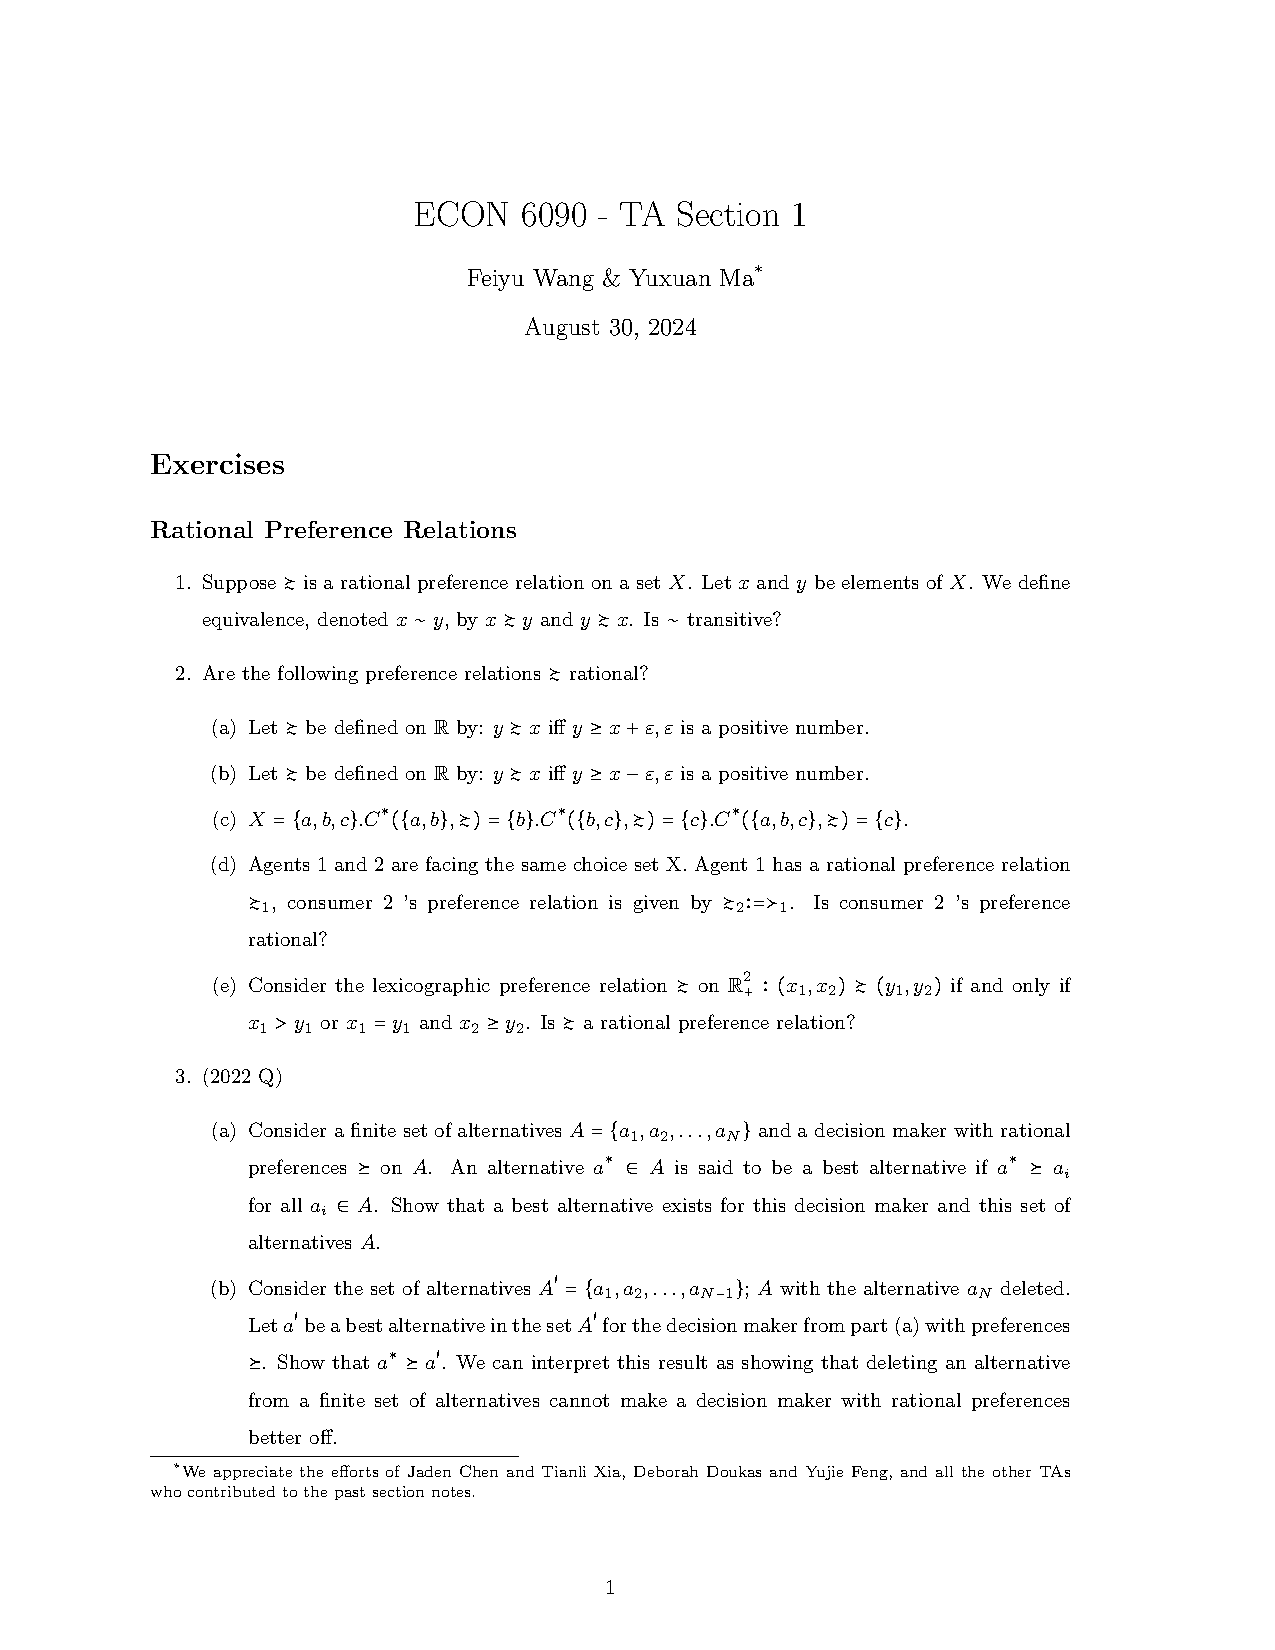
\includepdf[pages={-}]{_materials_fall_2024/ECON_6090/7._TA_Sections/ECON6090_TA_1.pdf}

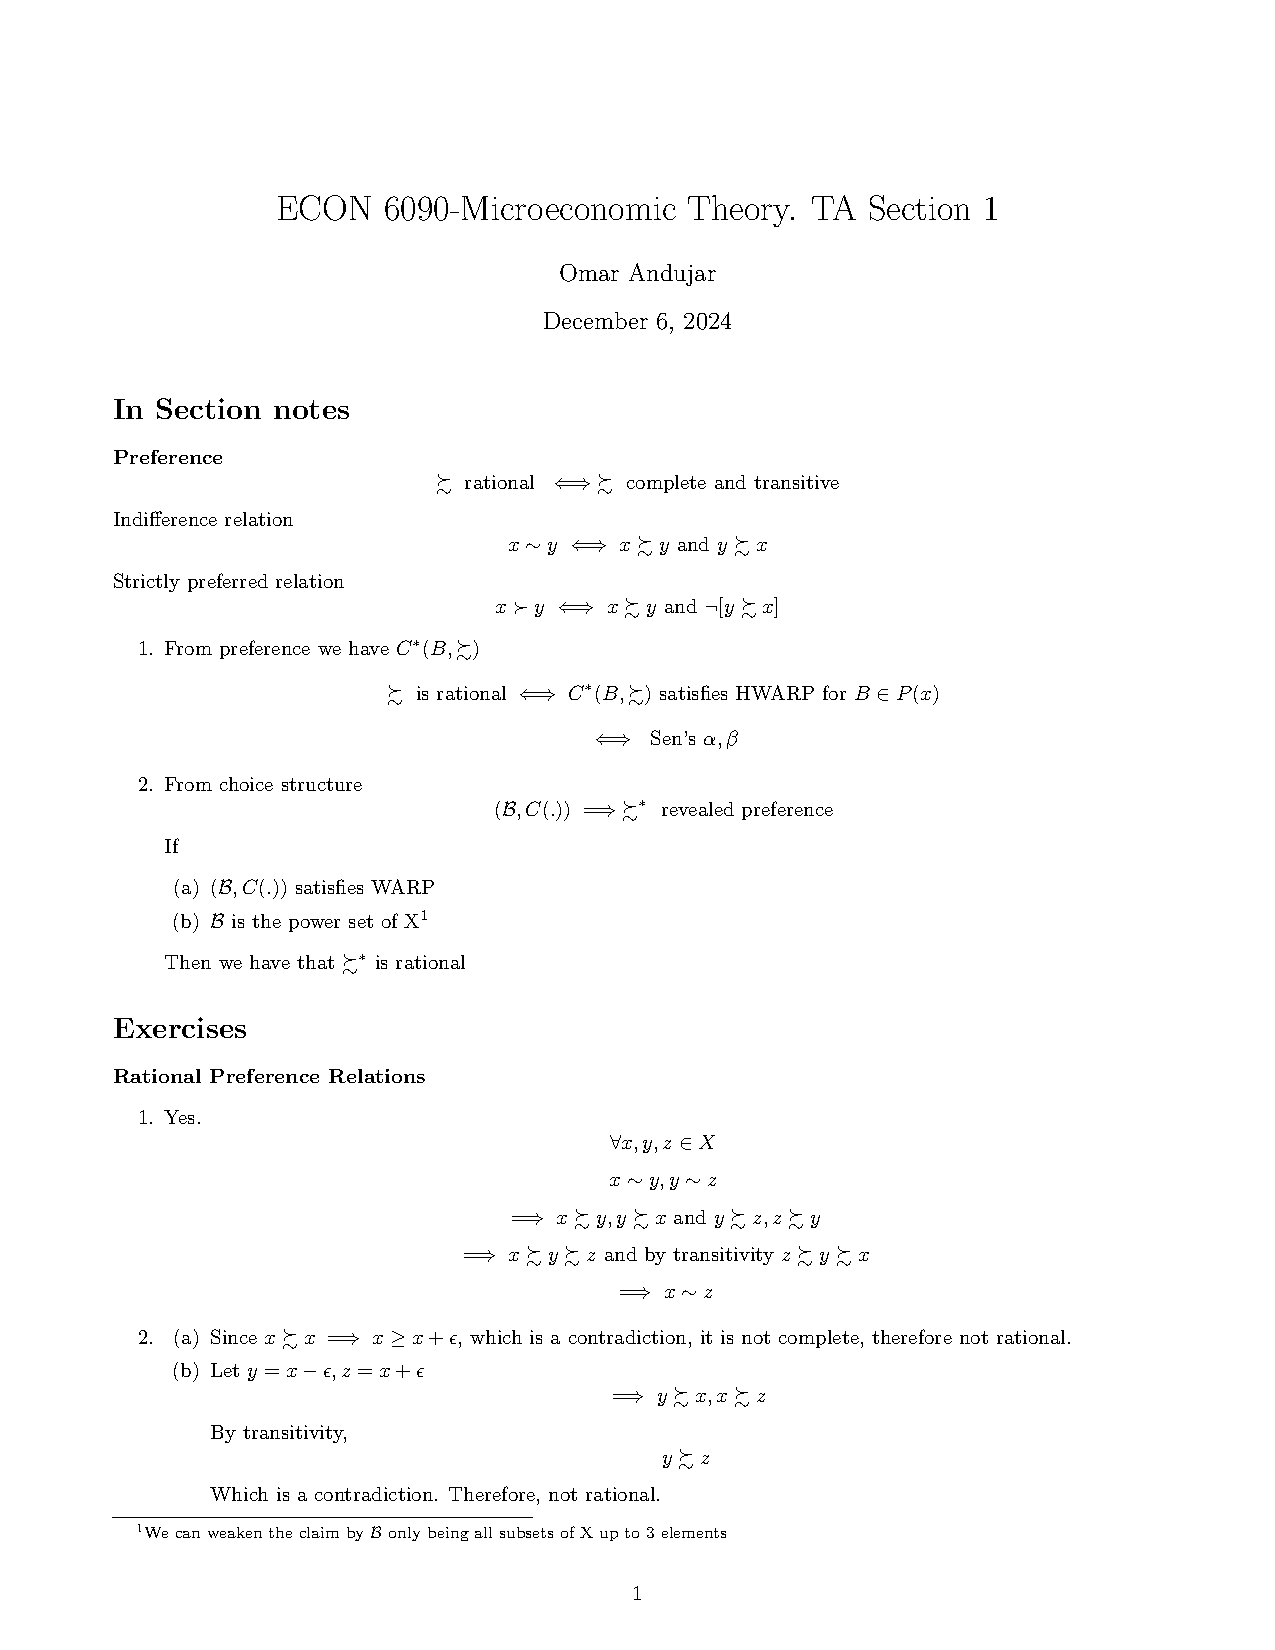
\includepdf[pages={-}]{_materials_fall_2024/ECON_6090/7._TA_Sections/Microeconomics_TASection1.pdf}

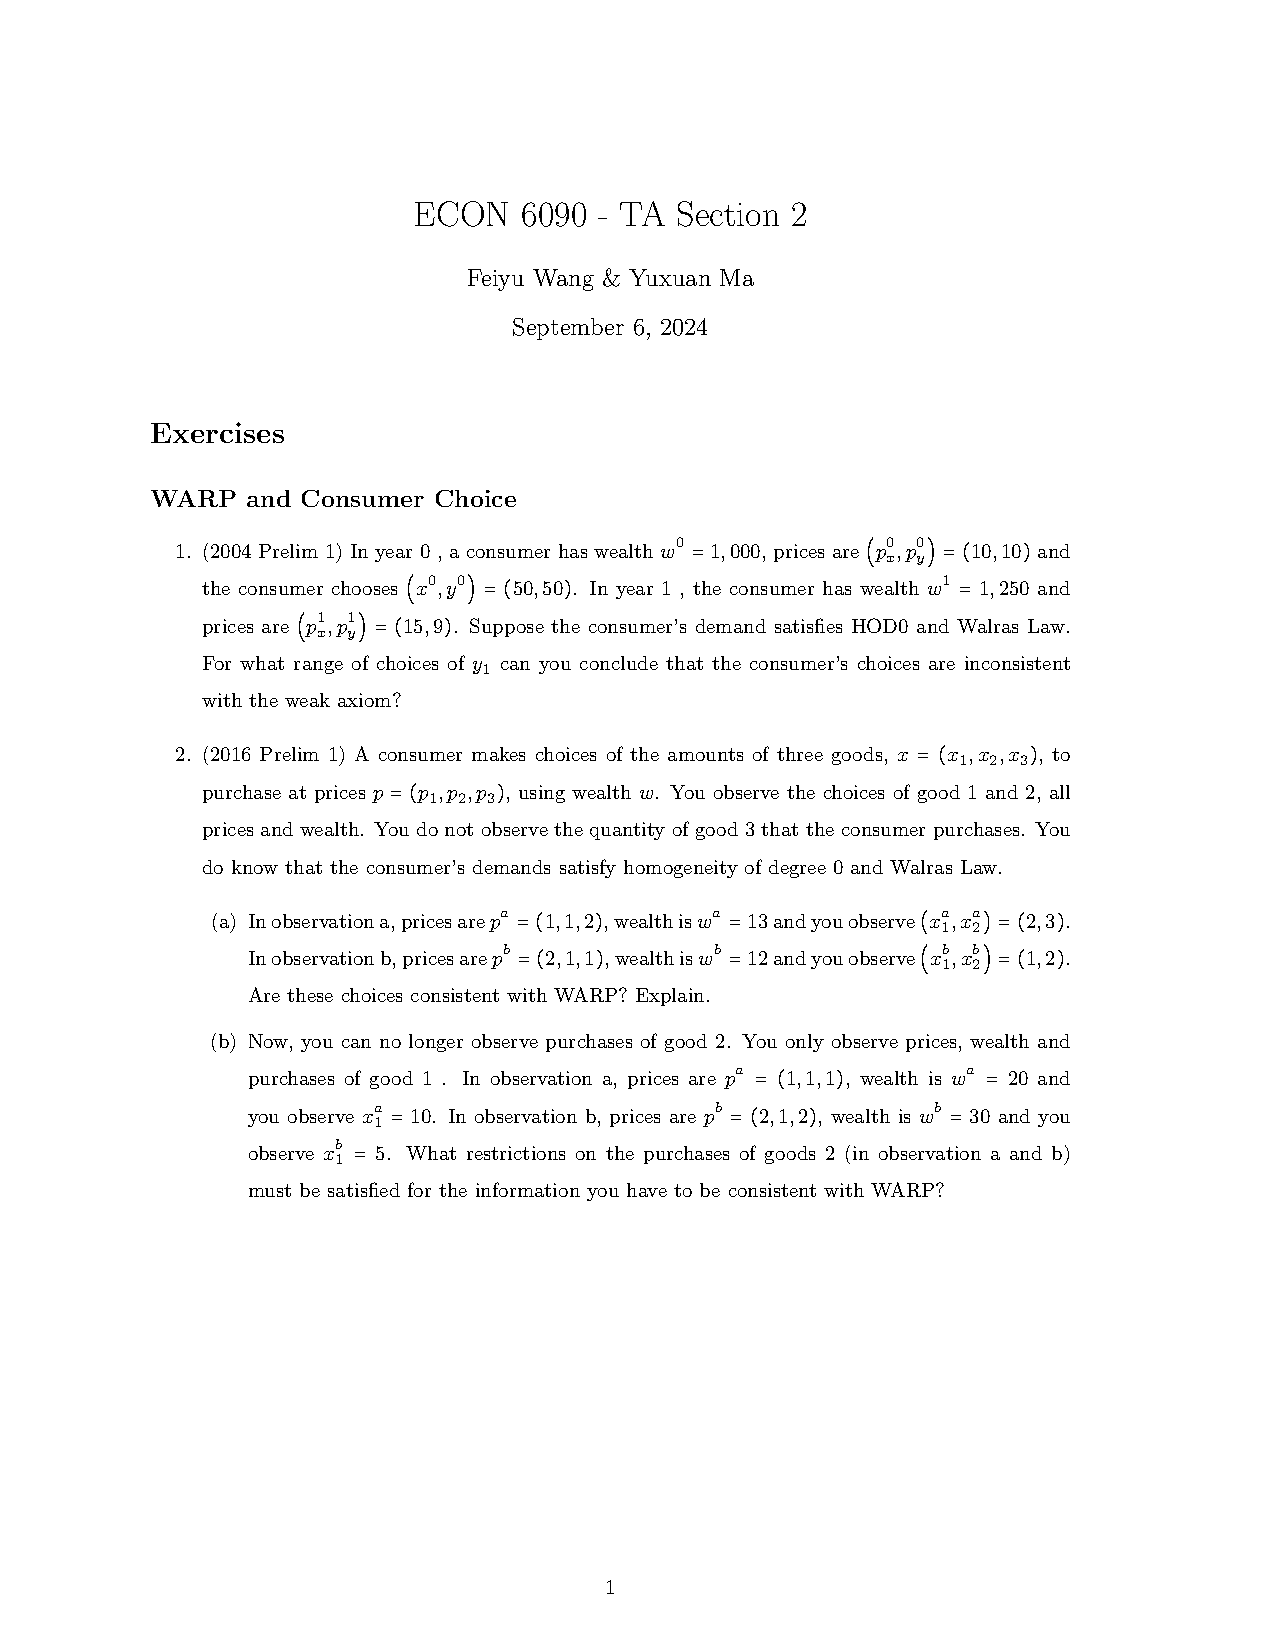
\includepdf[pages={-}]{_materials_fall_2024/ECON_6090/7._TA_Sections/ECON6090_TA_2.pdf}

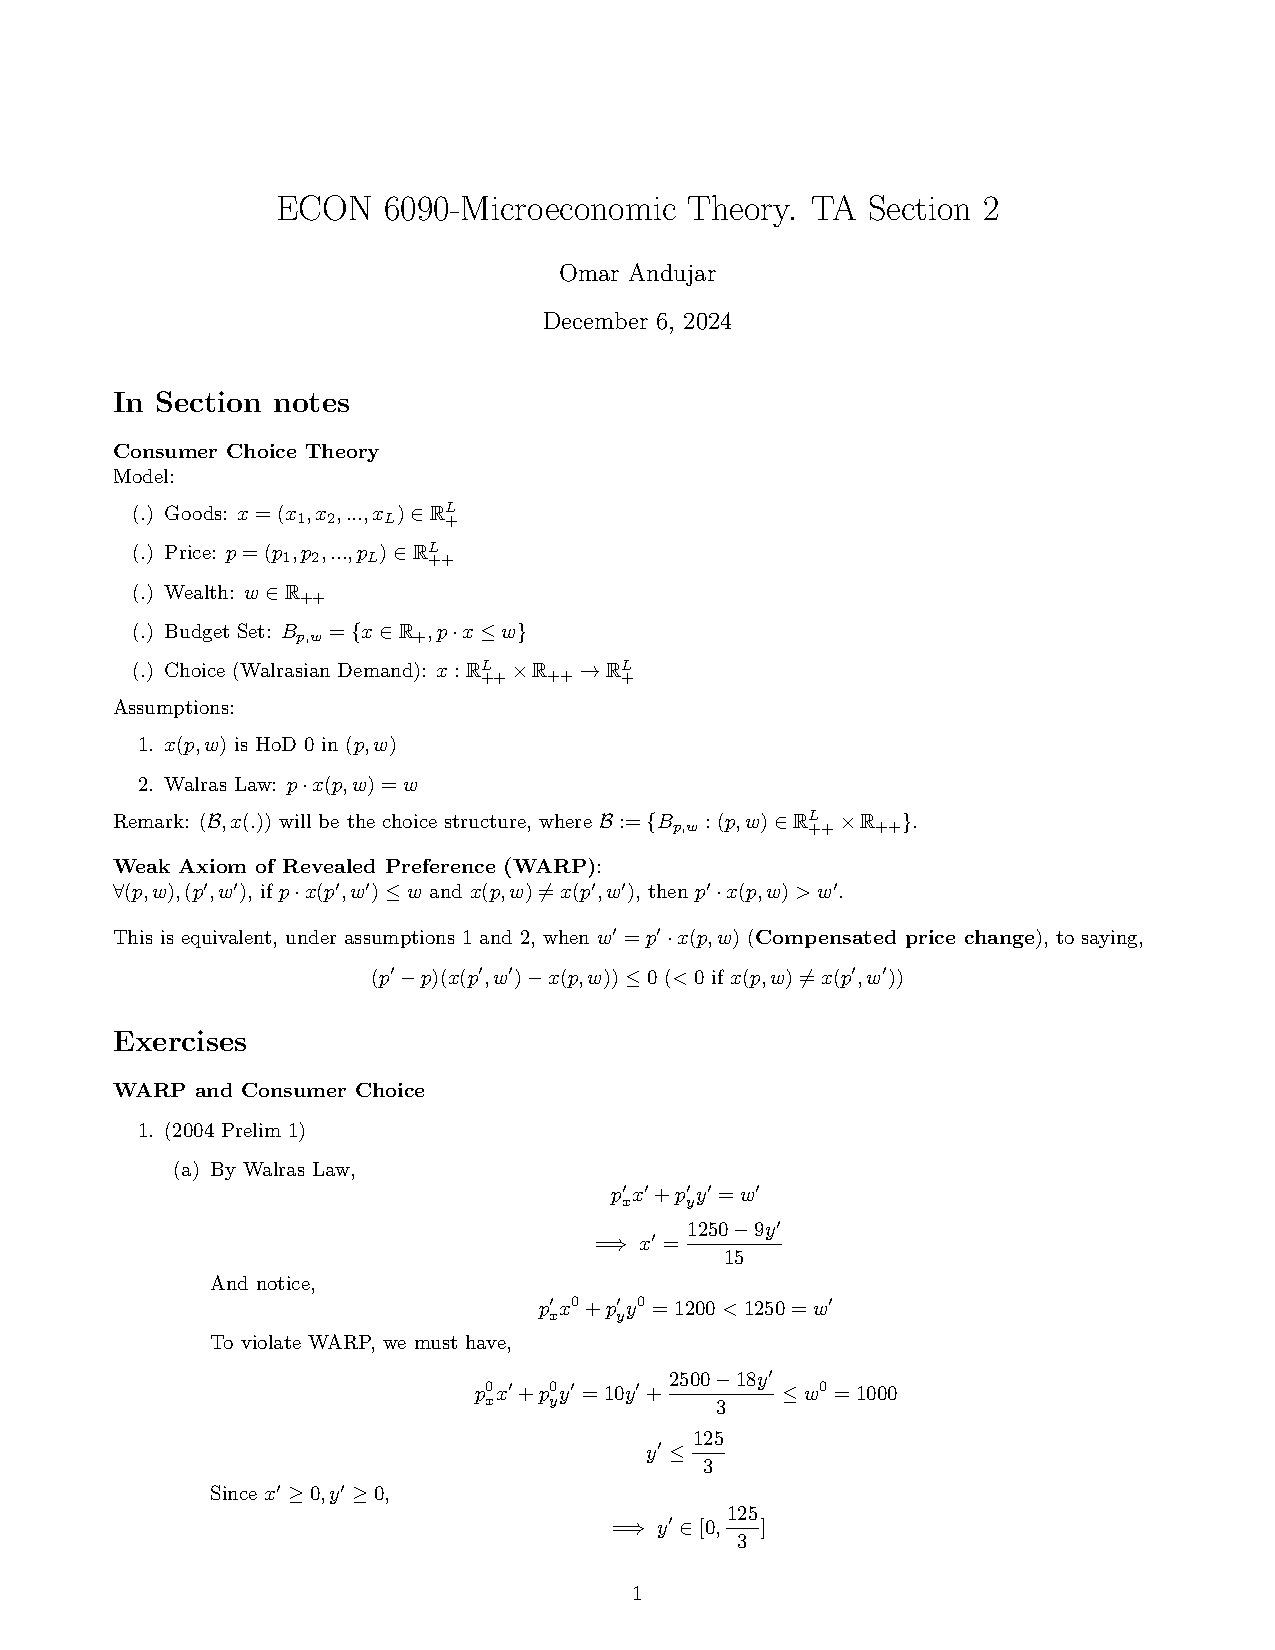
\includepdf[pages={-}]{_materials_fall_2024/ECON_6090/7._TA_Sections/Microeconomics_TASection2.pdf}

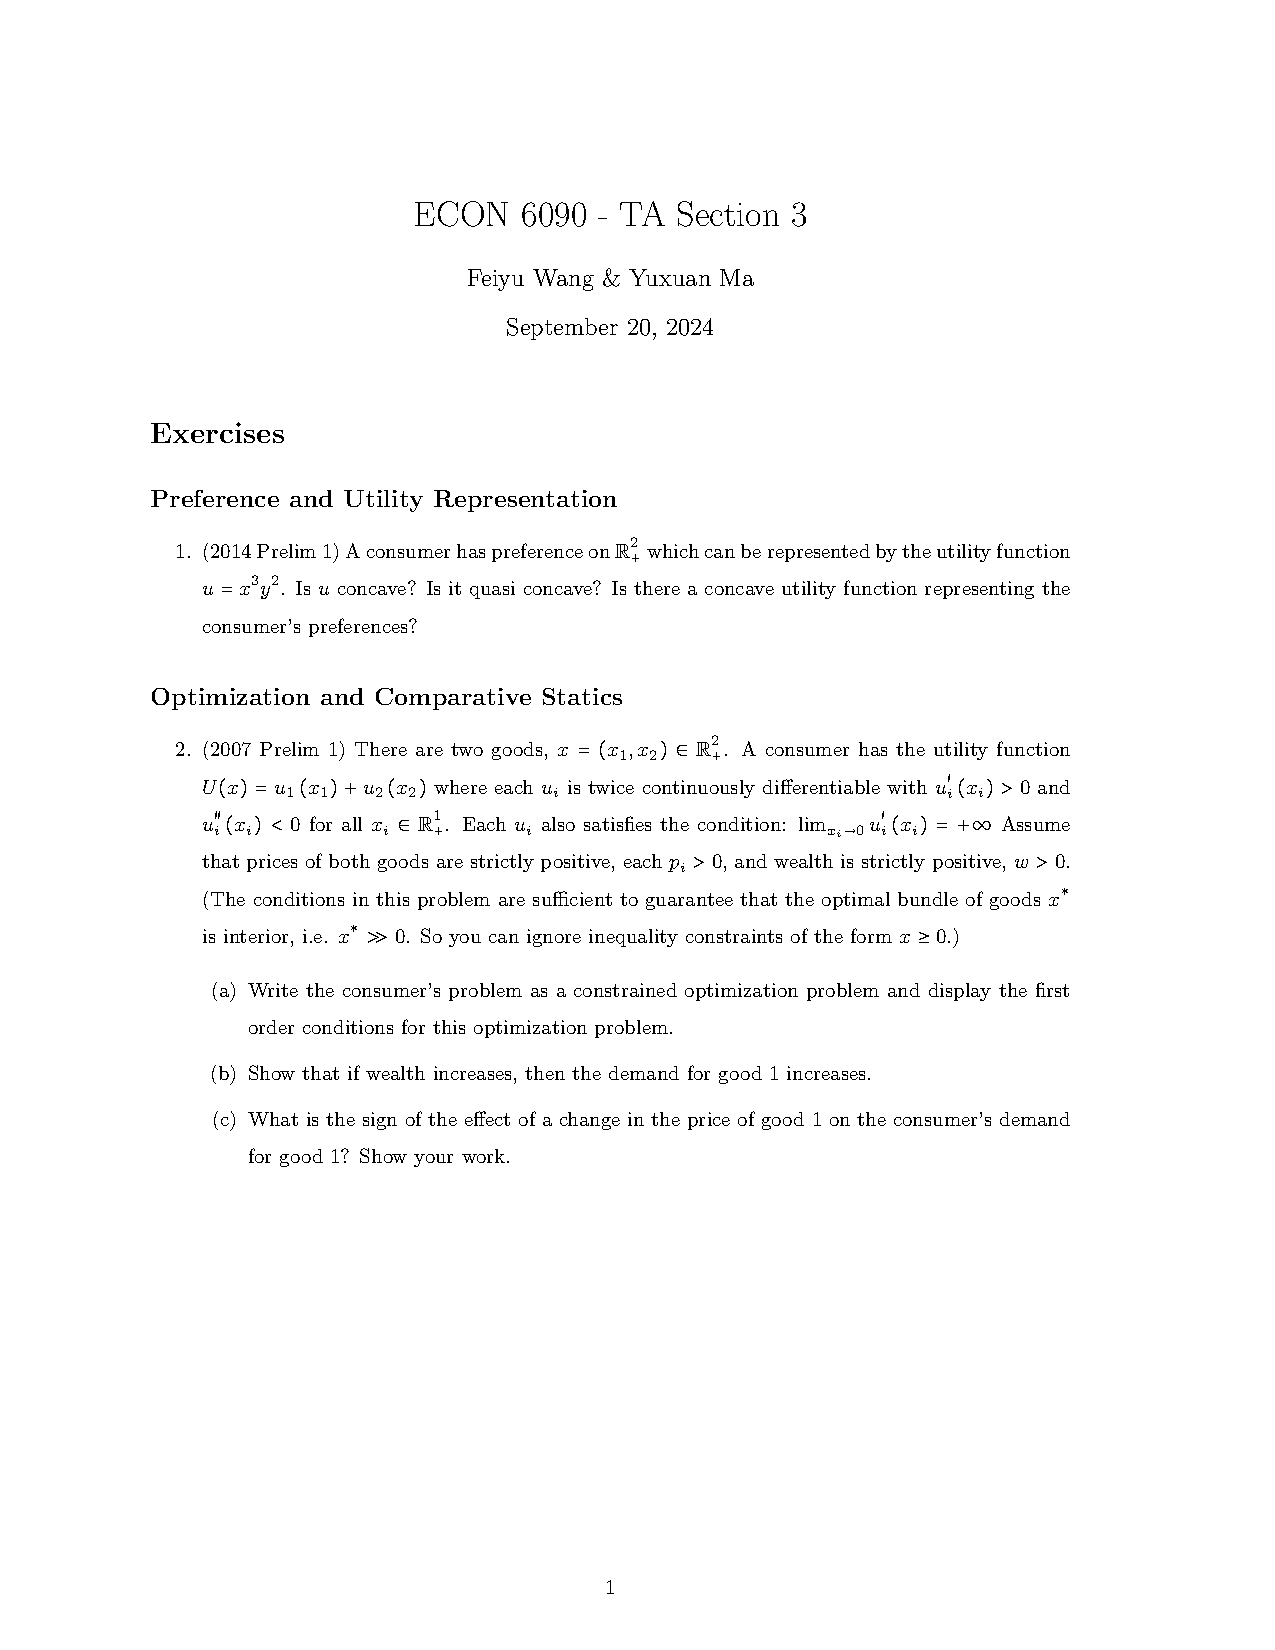
\includepdf[pages={-}]{_materials_fall_2024/ECON_6090/7._TA_Sections/ECON6090_TA_3.pdf}

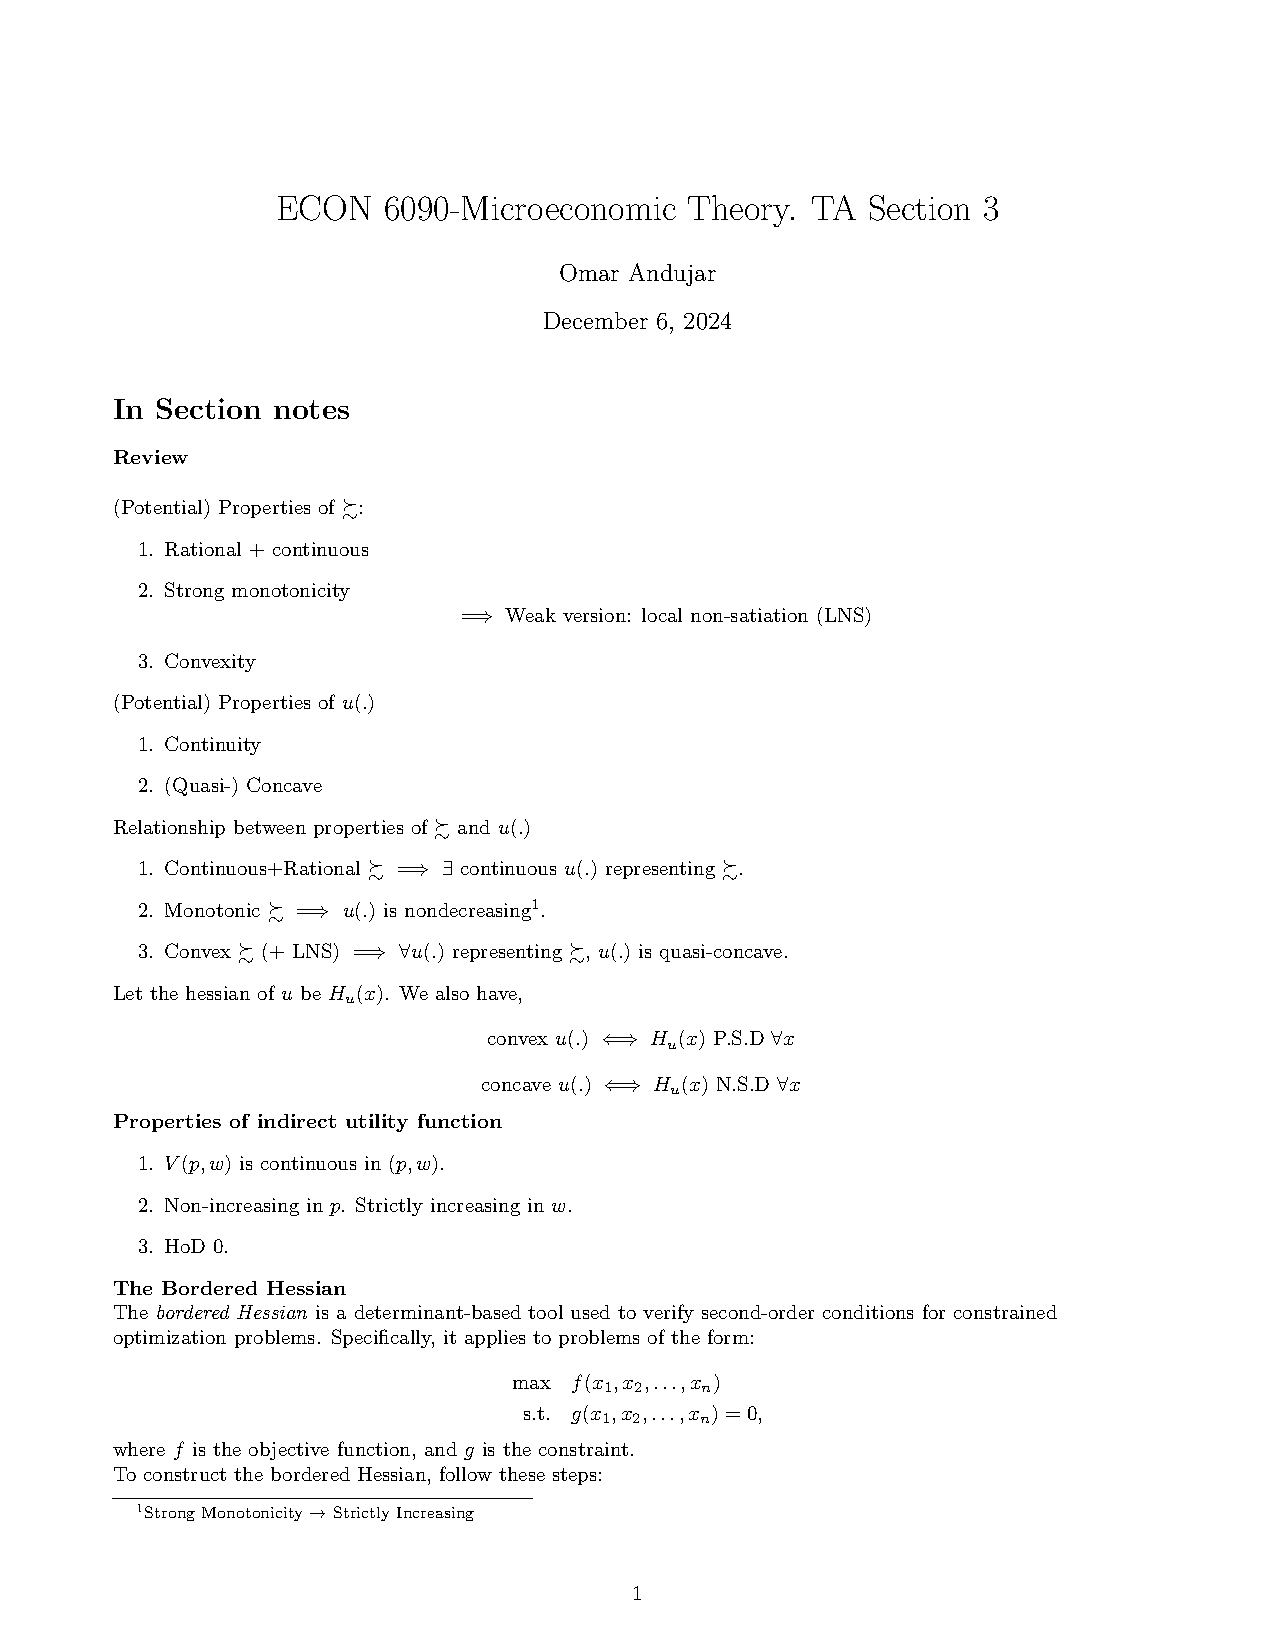
\includepdf[pages={-}]{_materials_fall_2024/ECON_6090/7._TA_Sections/Microeconomics_TASection3.pdf}

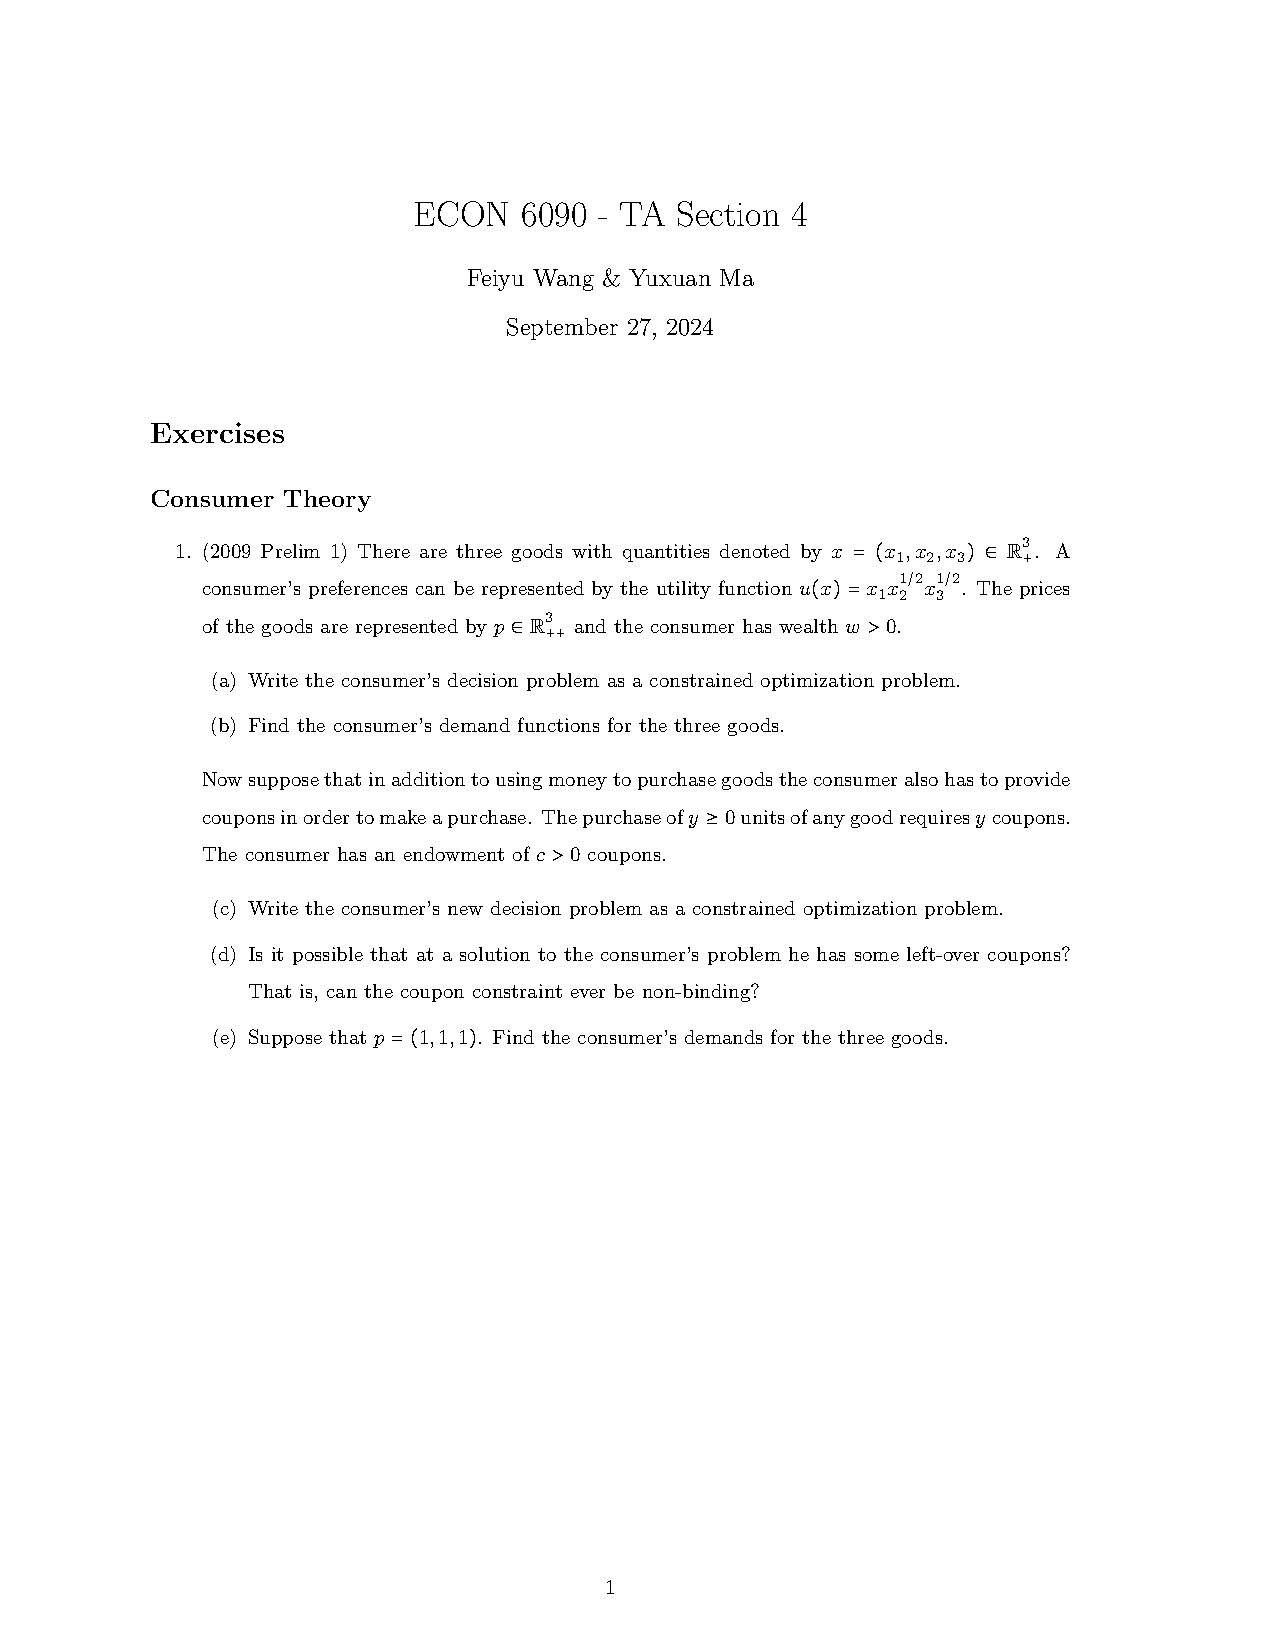
\includepdf[pages={-}]{_materials_fall_2024/ECON_6090/7._TA_Sections/ECON6090_TA_4.pdf}

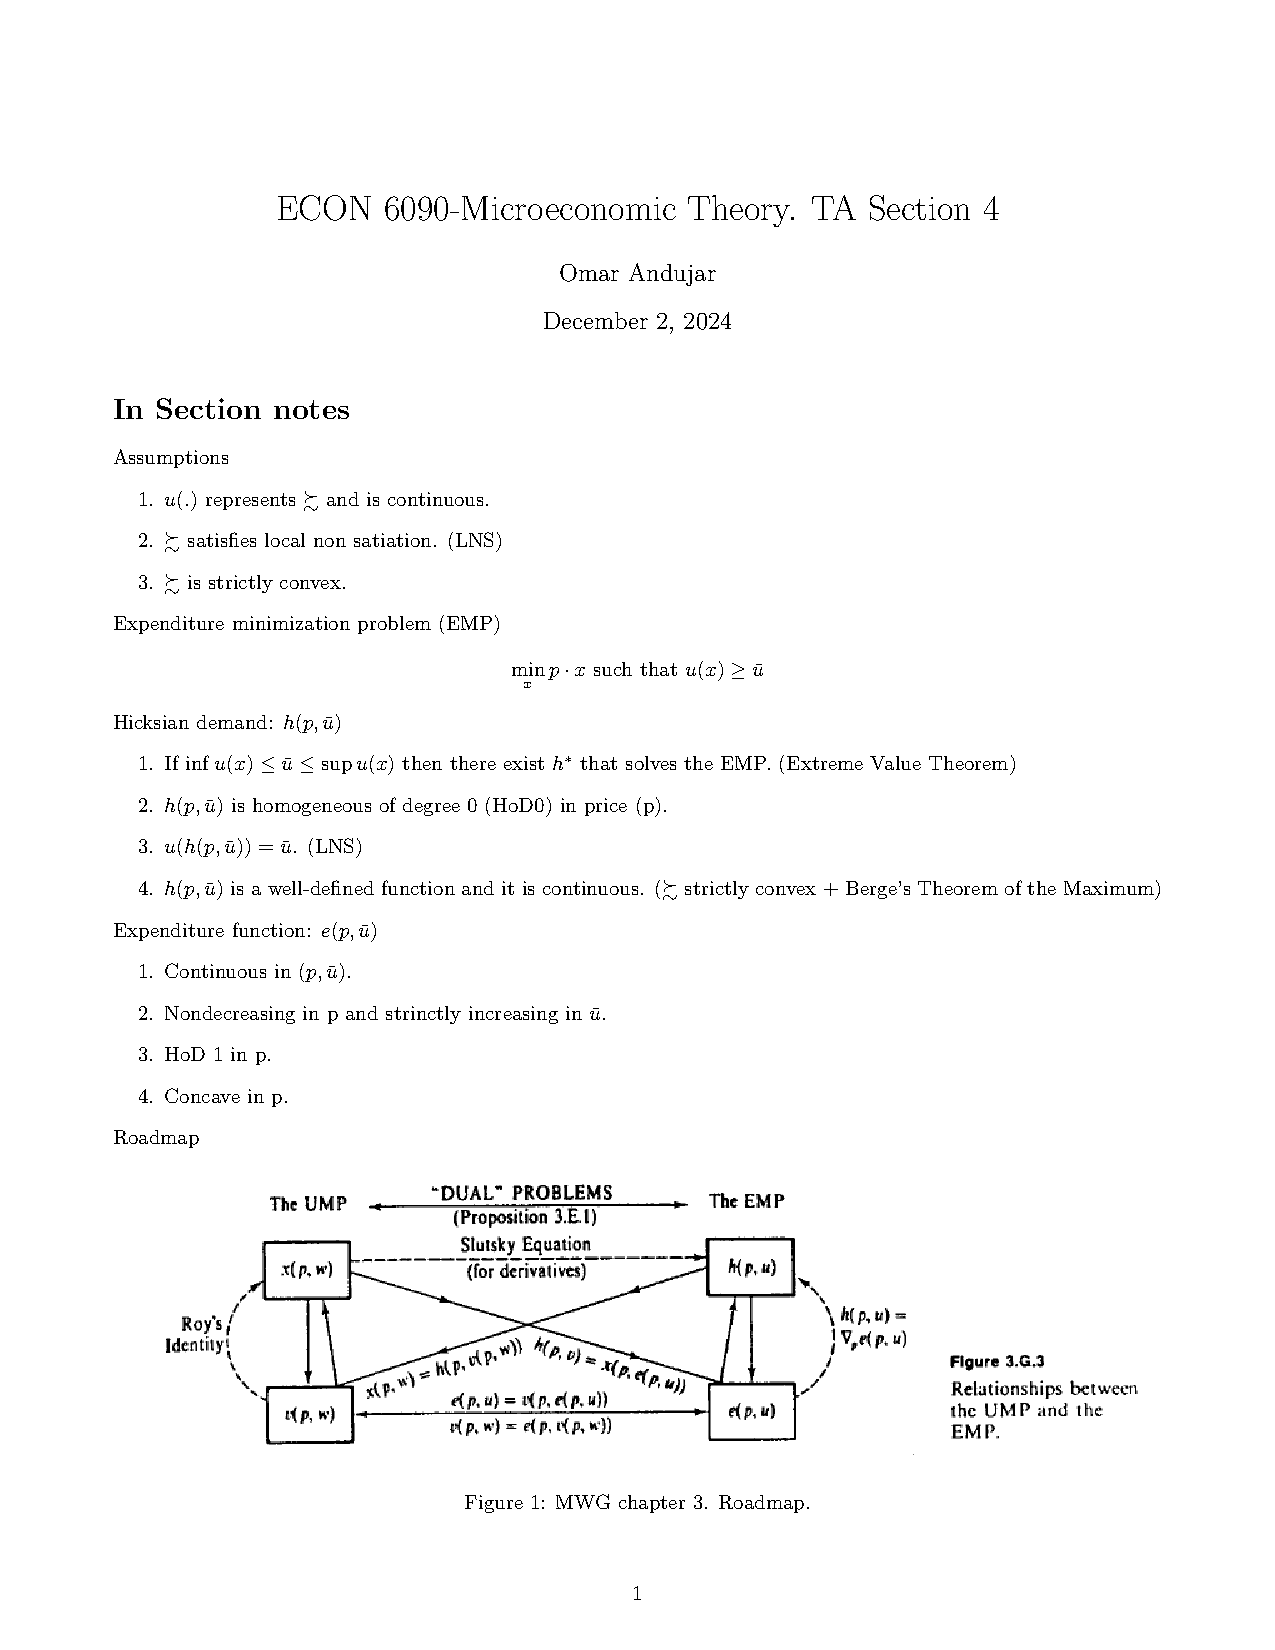
\includepdf[pages={-}]{_materials_fall_2024/ECON_6090/7._TA_Sections/Microeconomics_TASection4.pdf}

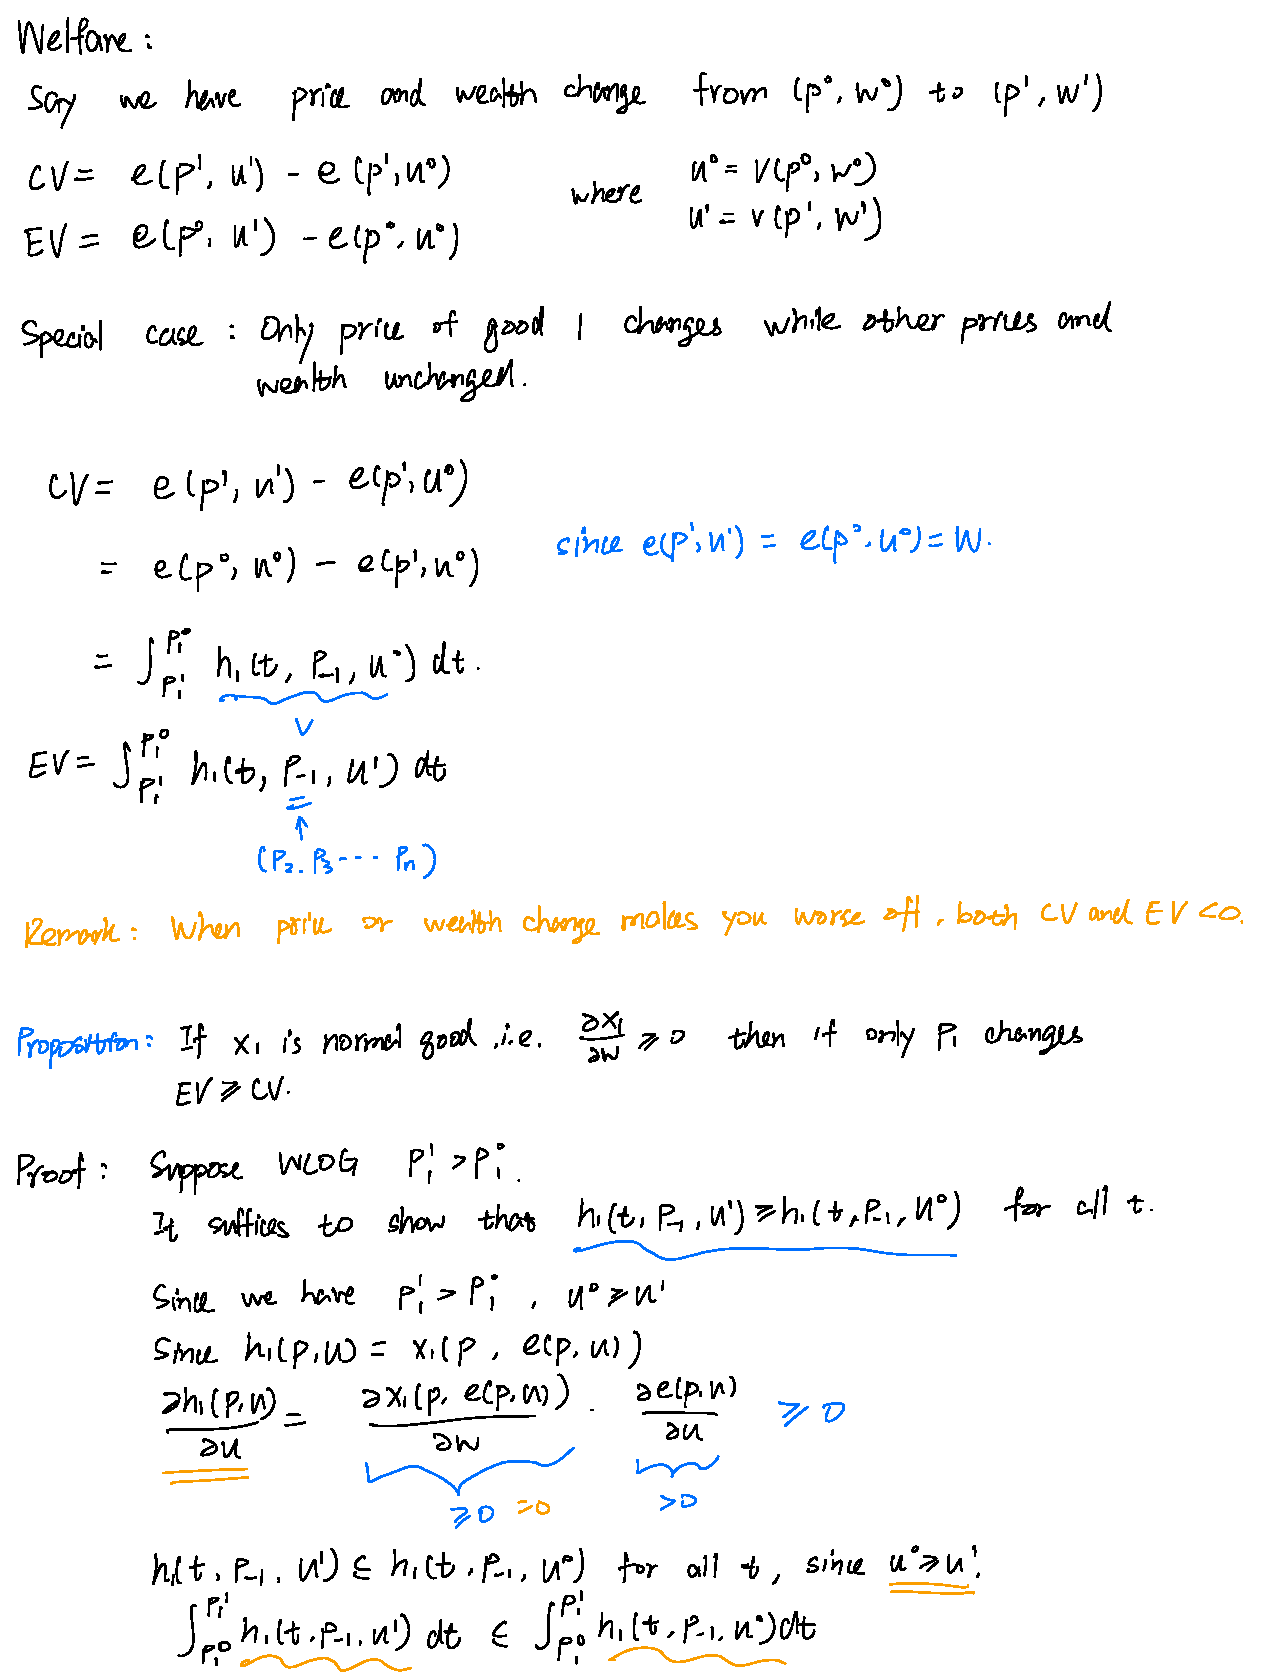
\includepdf[pages={-}]{_materials_fall_2024/ECON_6090/7._TA_Sections/ECON6090_TA_5.pdf}

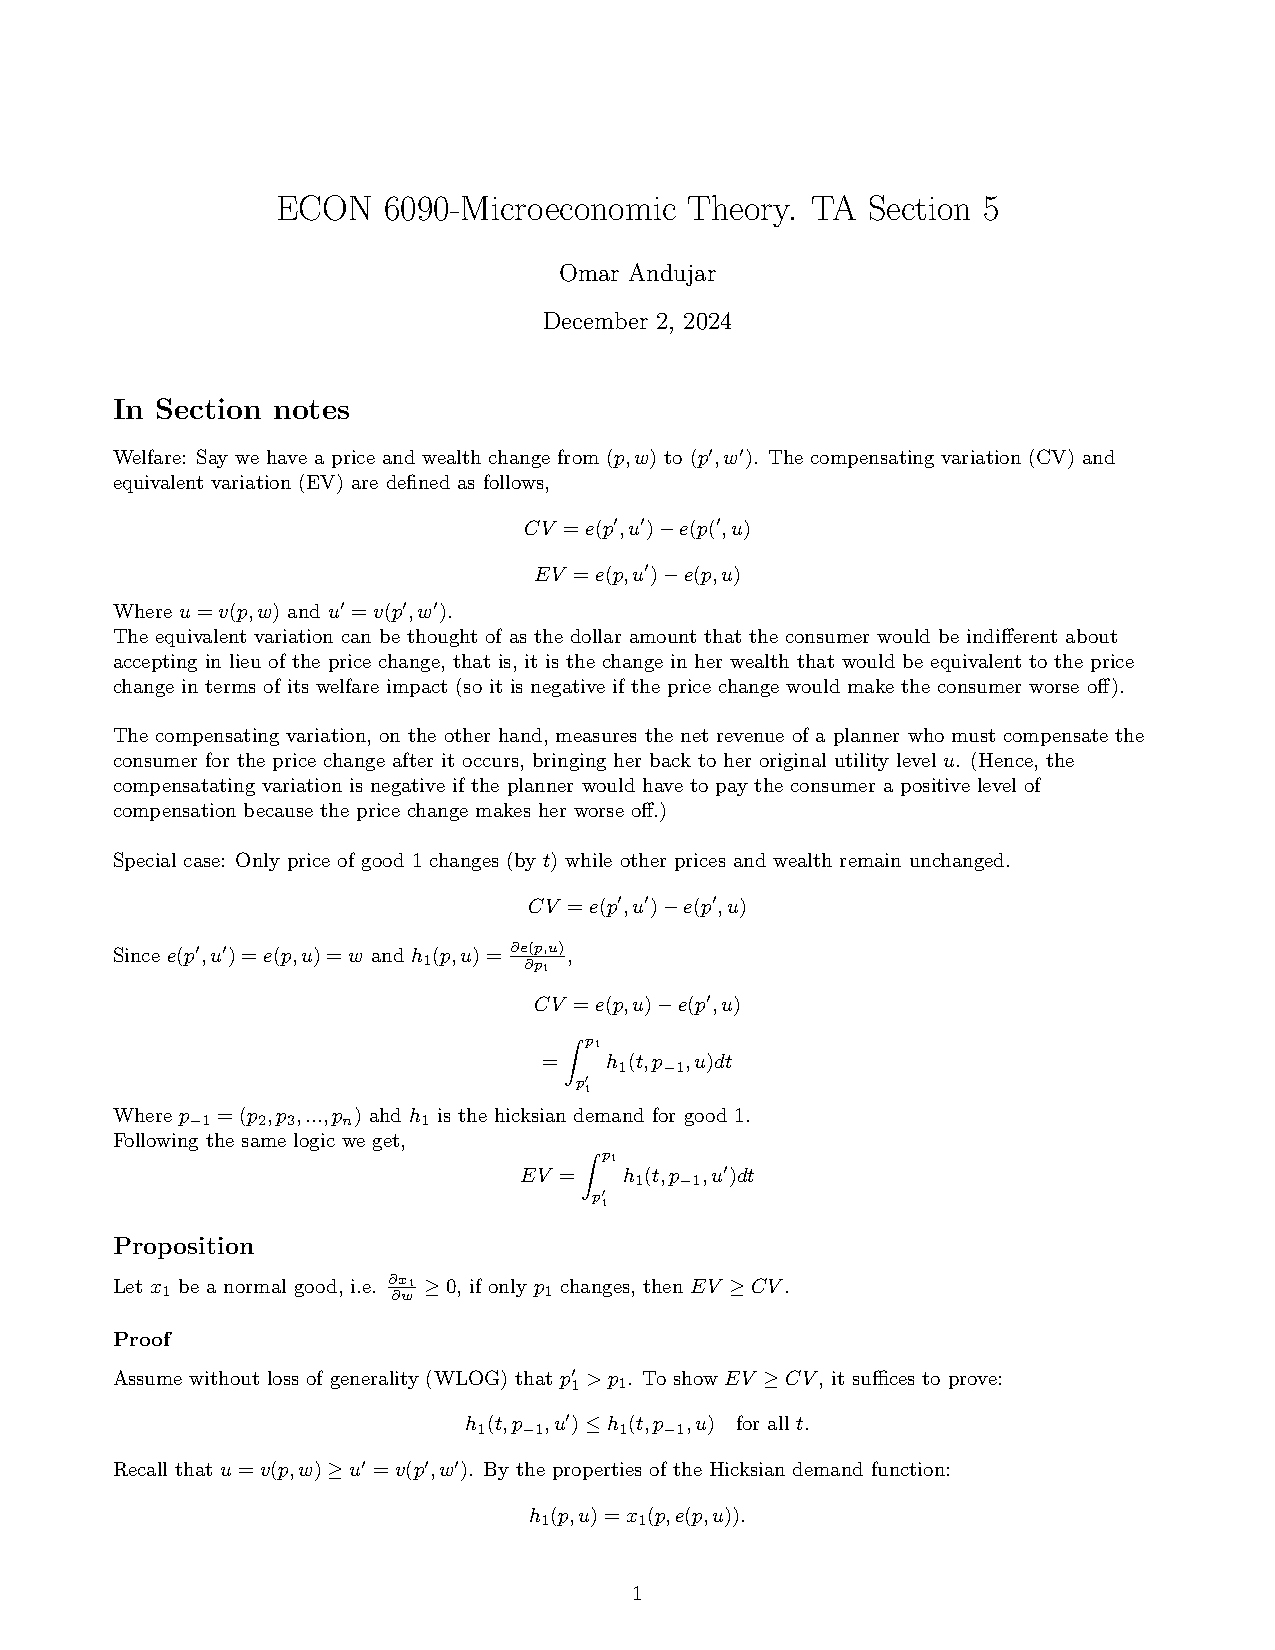
\includepdf[pages={-}]{_materials_fall_2024/ECON_6090/7._TA_Sections/Microeconomics_TASection5.pdf}

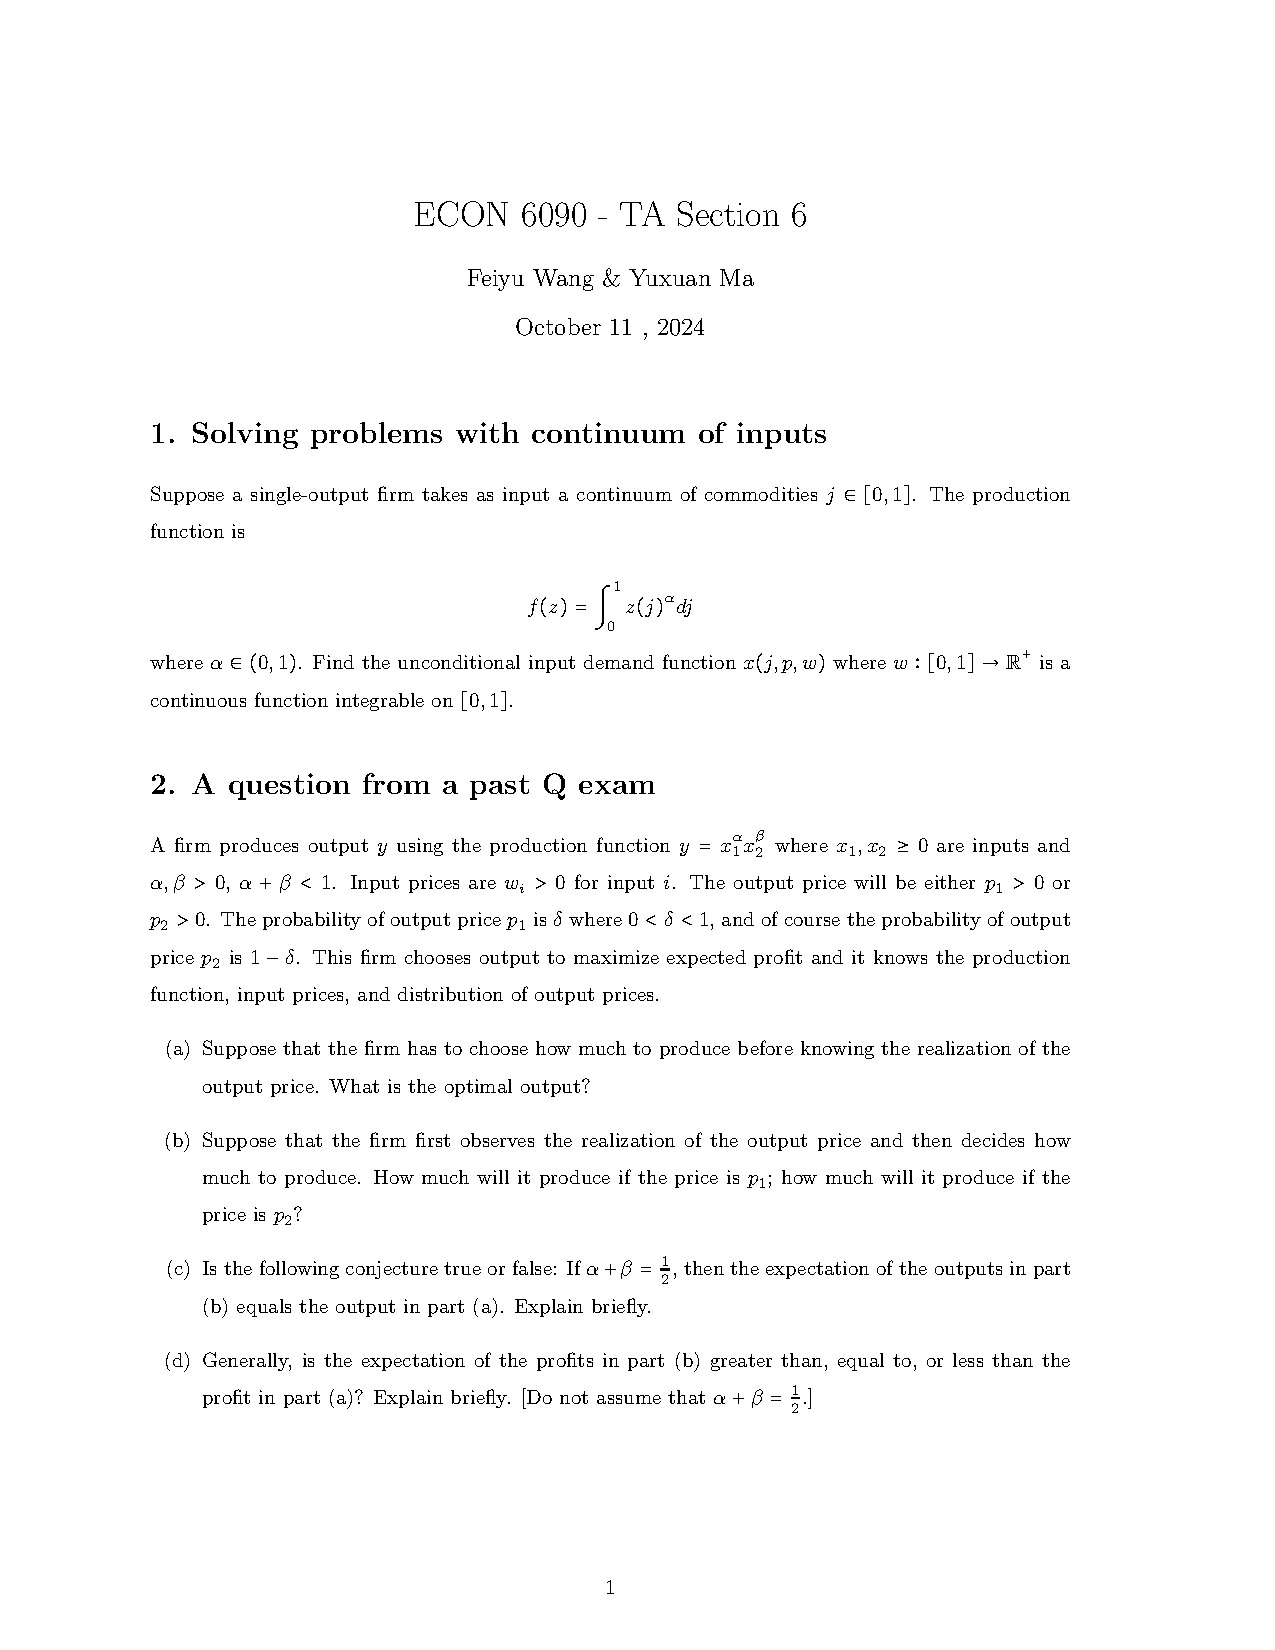
\includepdf[pages={-}]{_materials_fall_2024/ECON_6090/7._TA_Sections/ECON6090_TA_6.pdf}

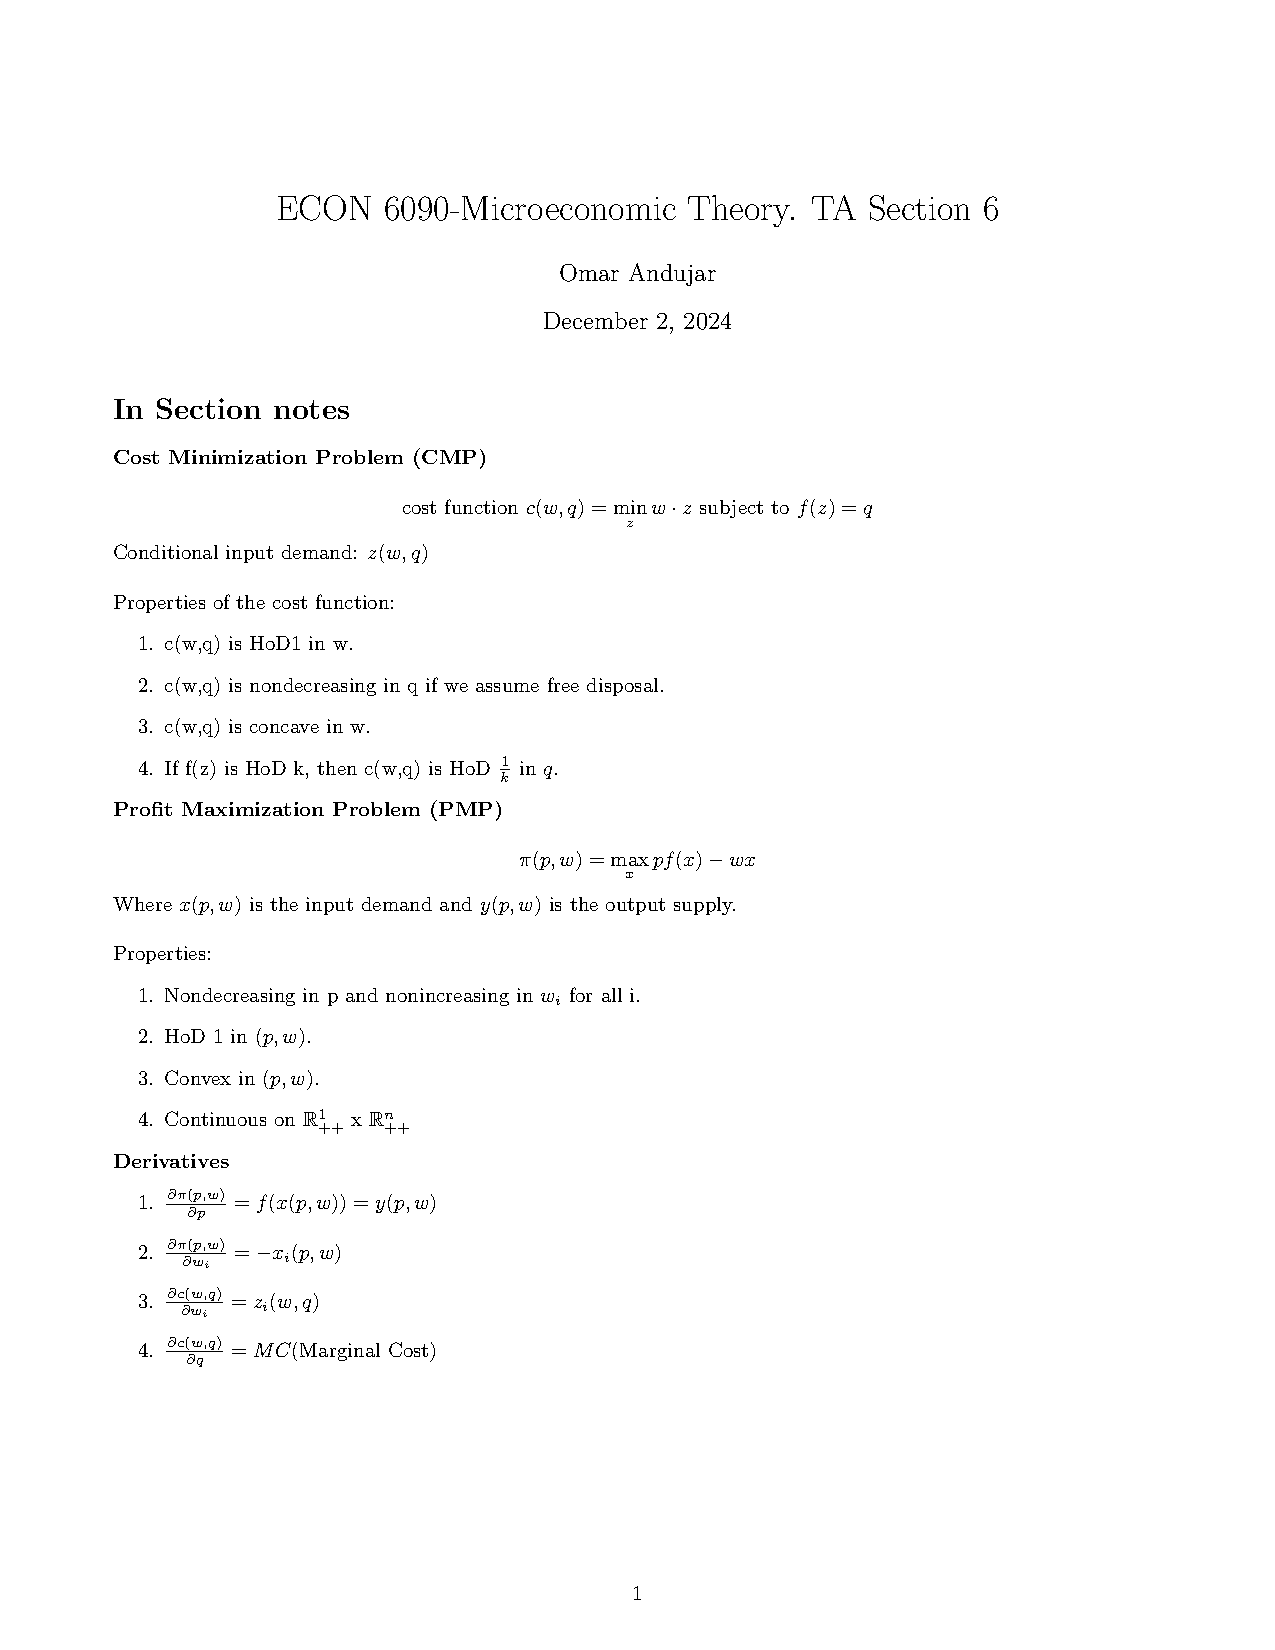
\includepdf[pages={-}]{_materials_fall_2024/ECON_6090/7._TA_Sections/Microeconomics_TASection6.pdf}

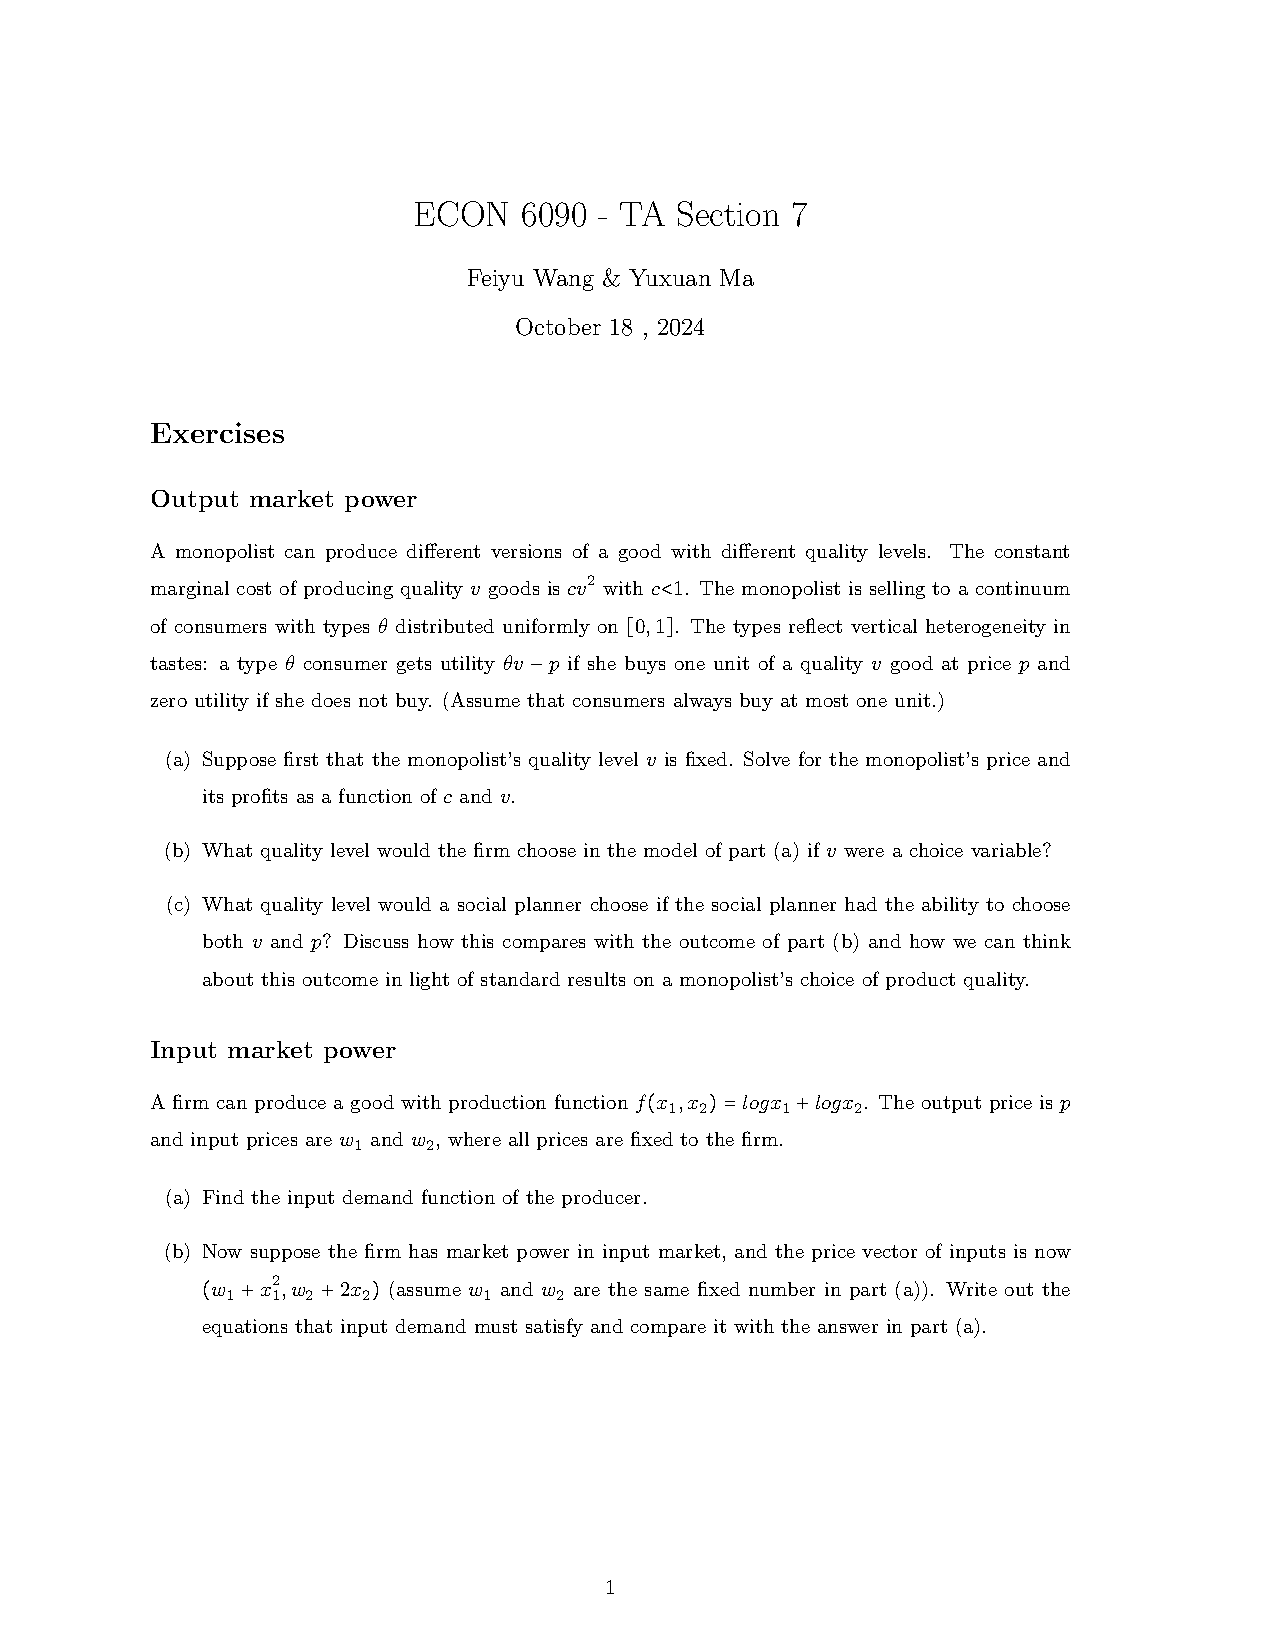
\includepdf[pages={-}]{_materials_fall_2024/ECON_6090/7._TA_Sections/ECON6090_TA_7.pdf}

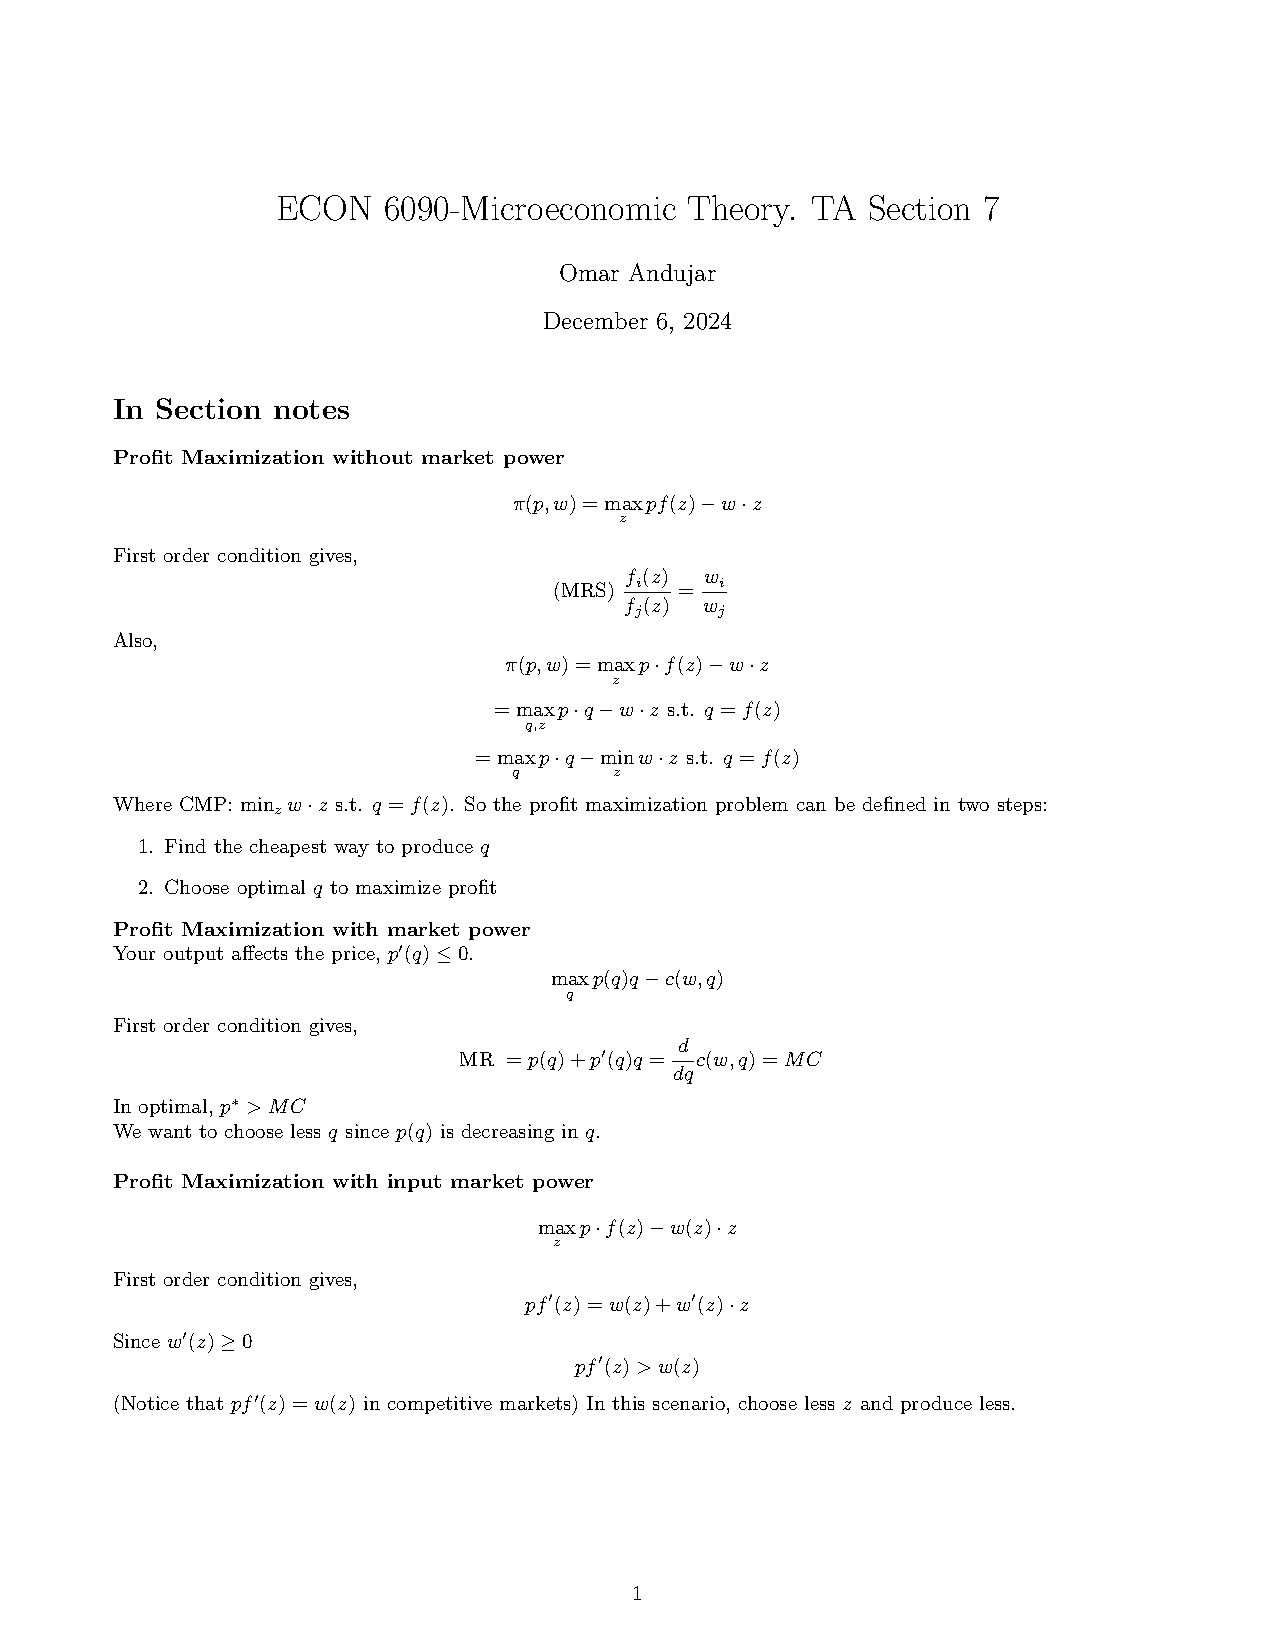
\includepdf[pages={-}]{_materials_fall_2024/ECON_6090/7._TA_Sections/Microeconomics_TASection7.pdf}

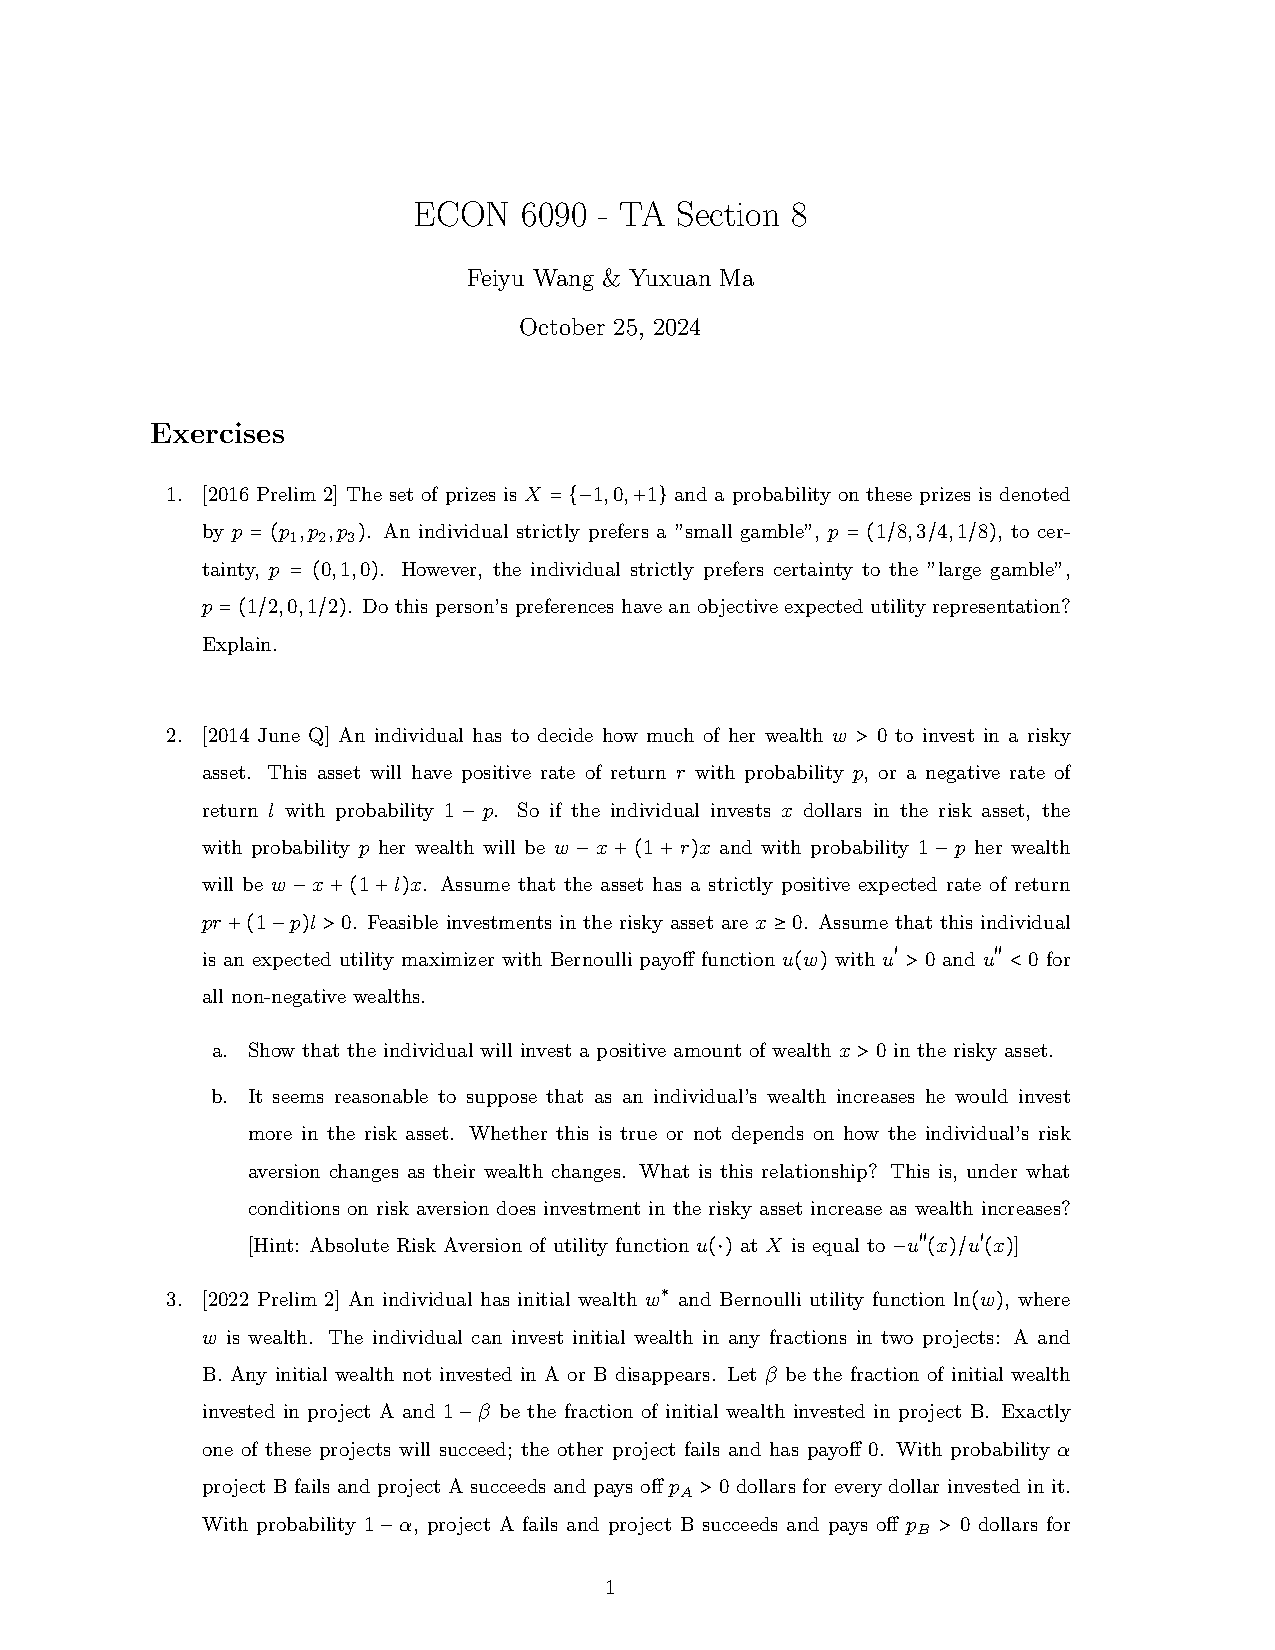
\includepdf[pages={-}]{_materials_fall_2024/ECON_6090/7._TA_Sections/ECON6090_TA_8.pdf}

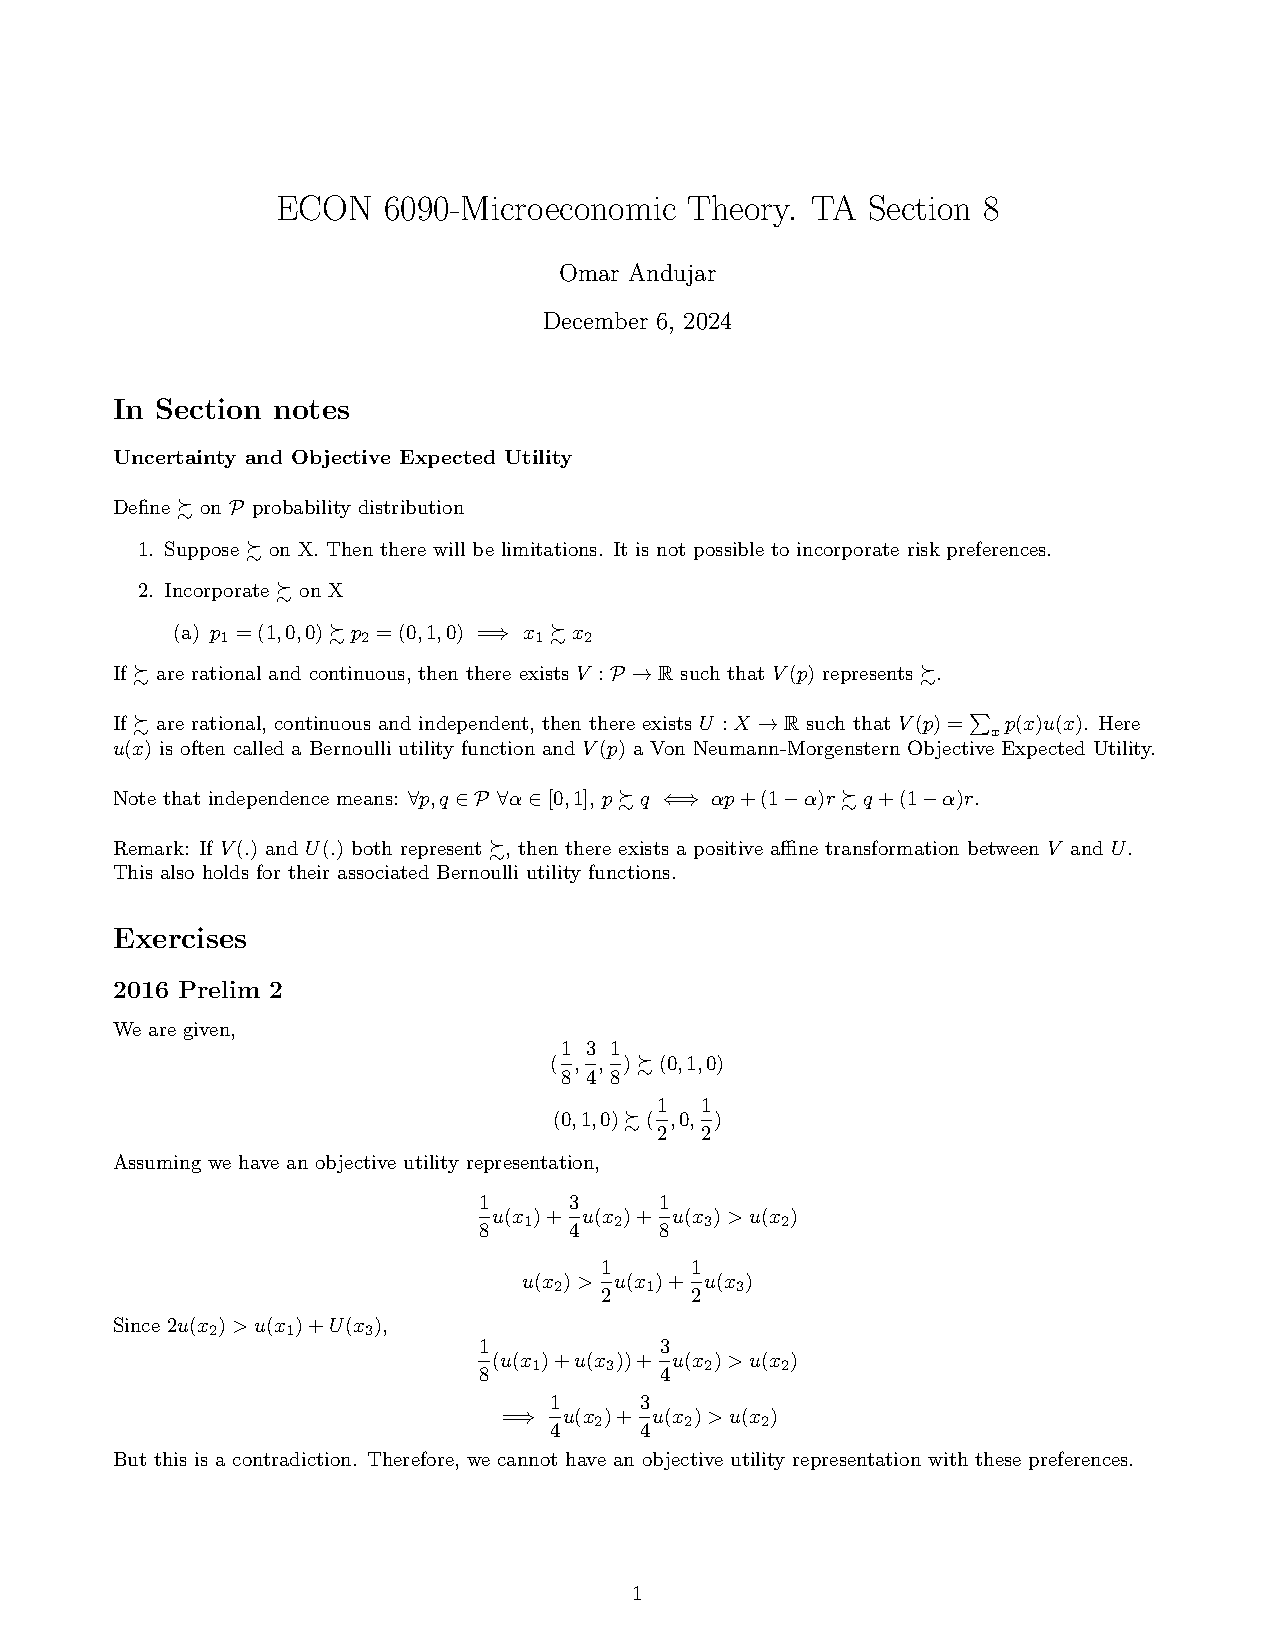
\includepdf[pages={-}]{_materials_fall_2024/ECON_6090/7._TA_Sections/Microeconomics_TASection8.pdf}

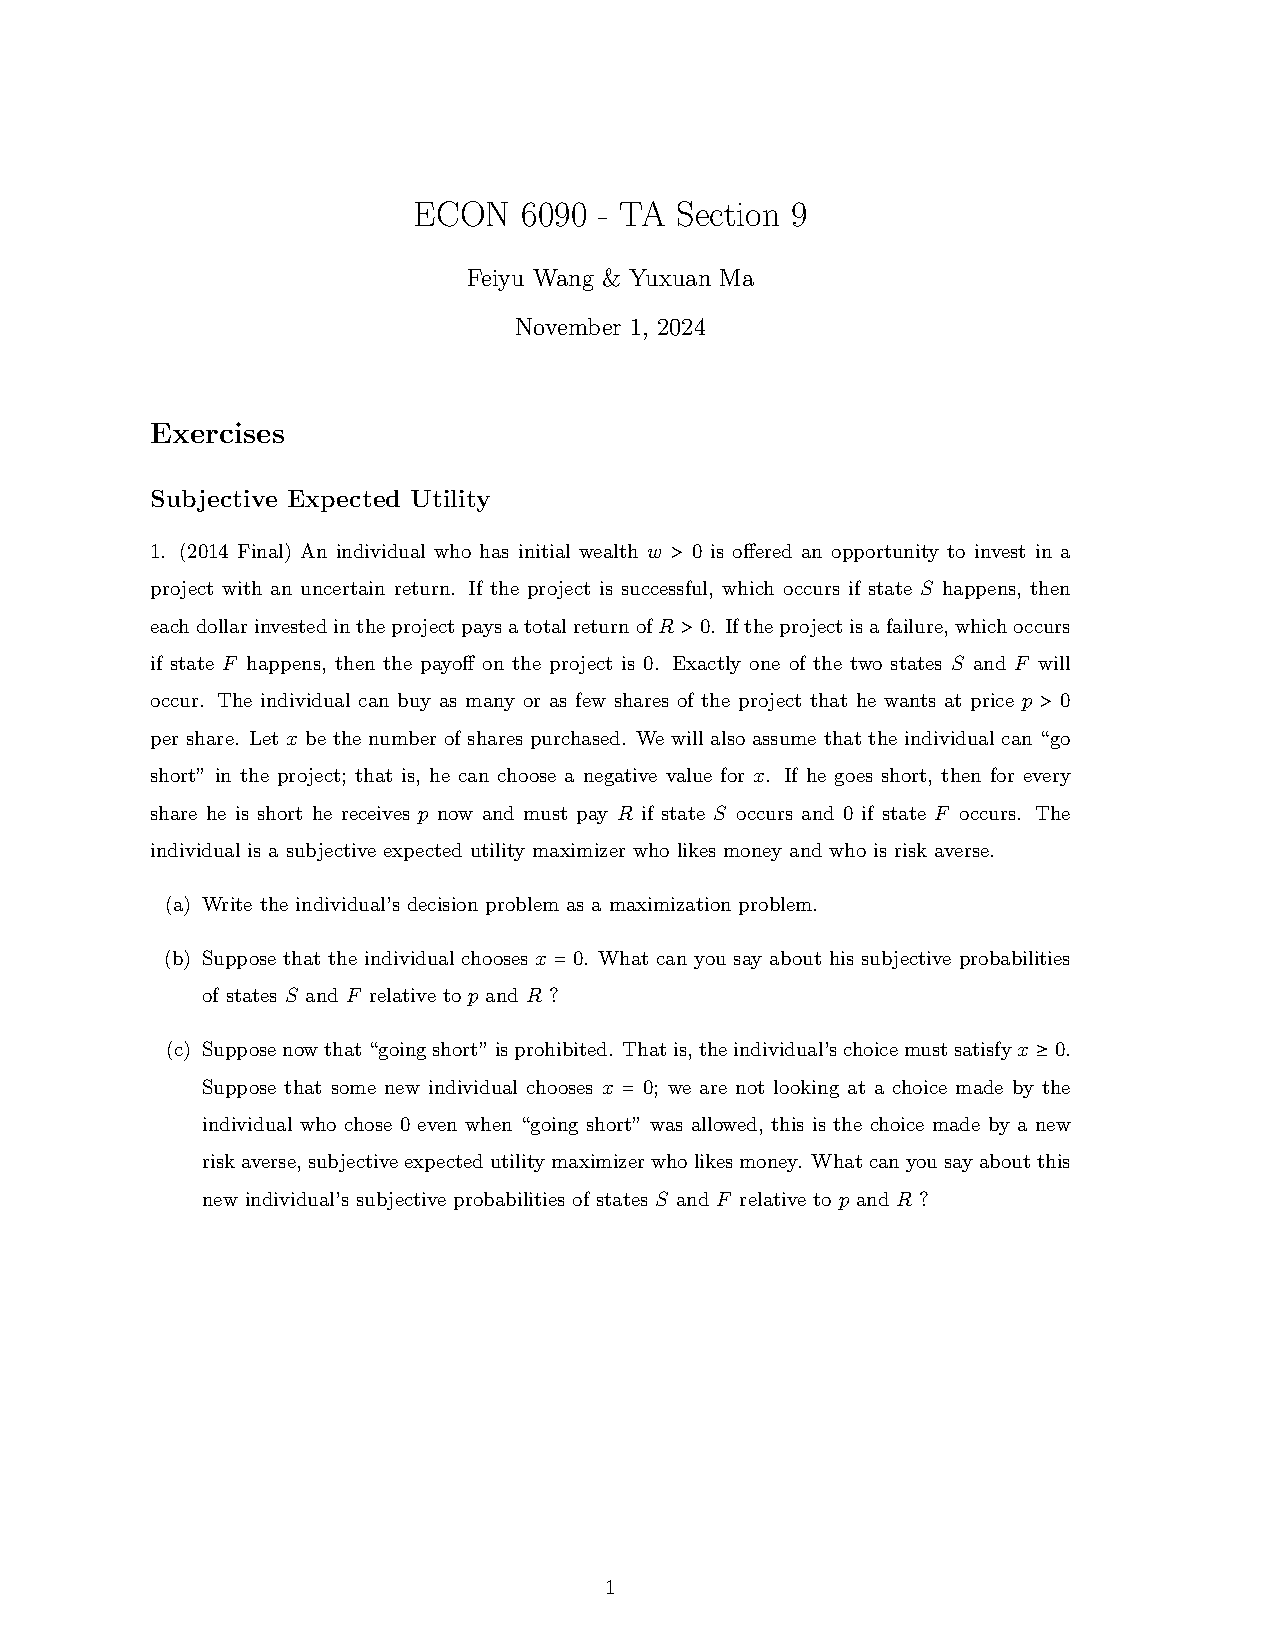
\includepdf[pages={-}]{_materials_fall_2024/ECON_6090/7._TA_Sections/ECON6090_TA_9.pdf}

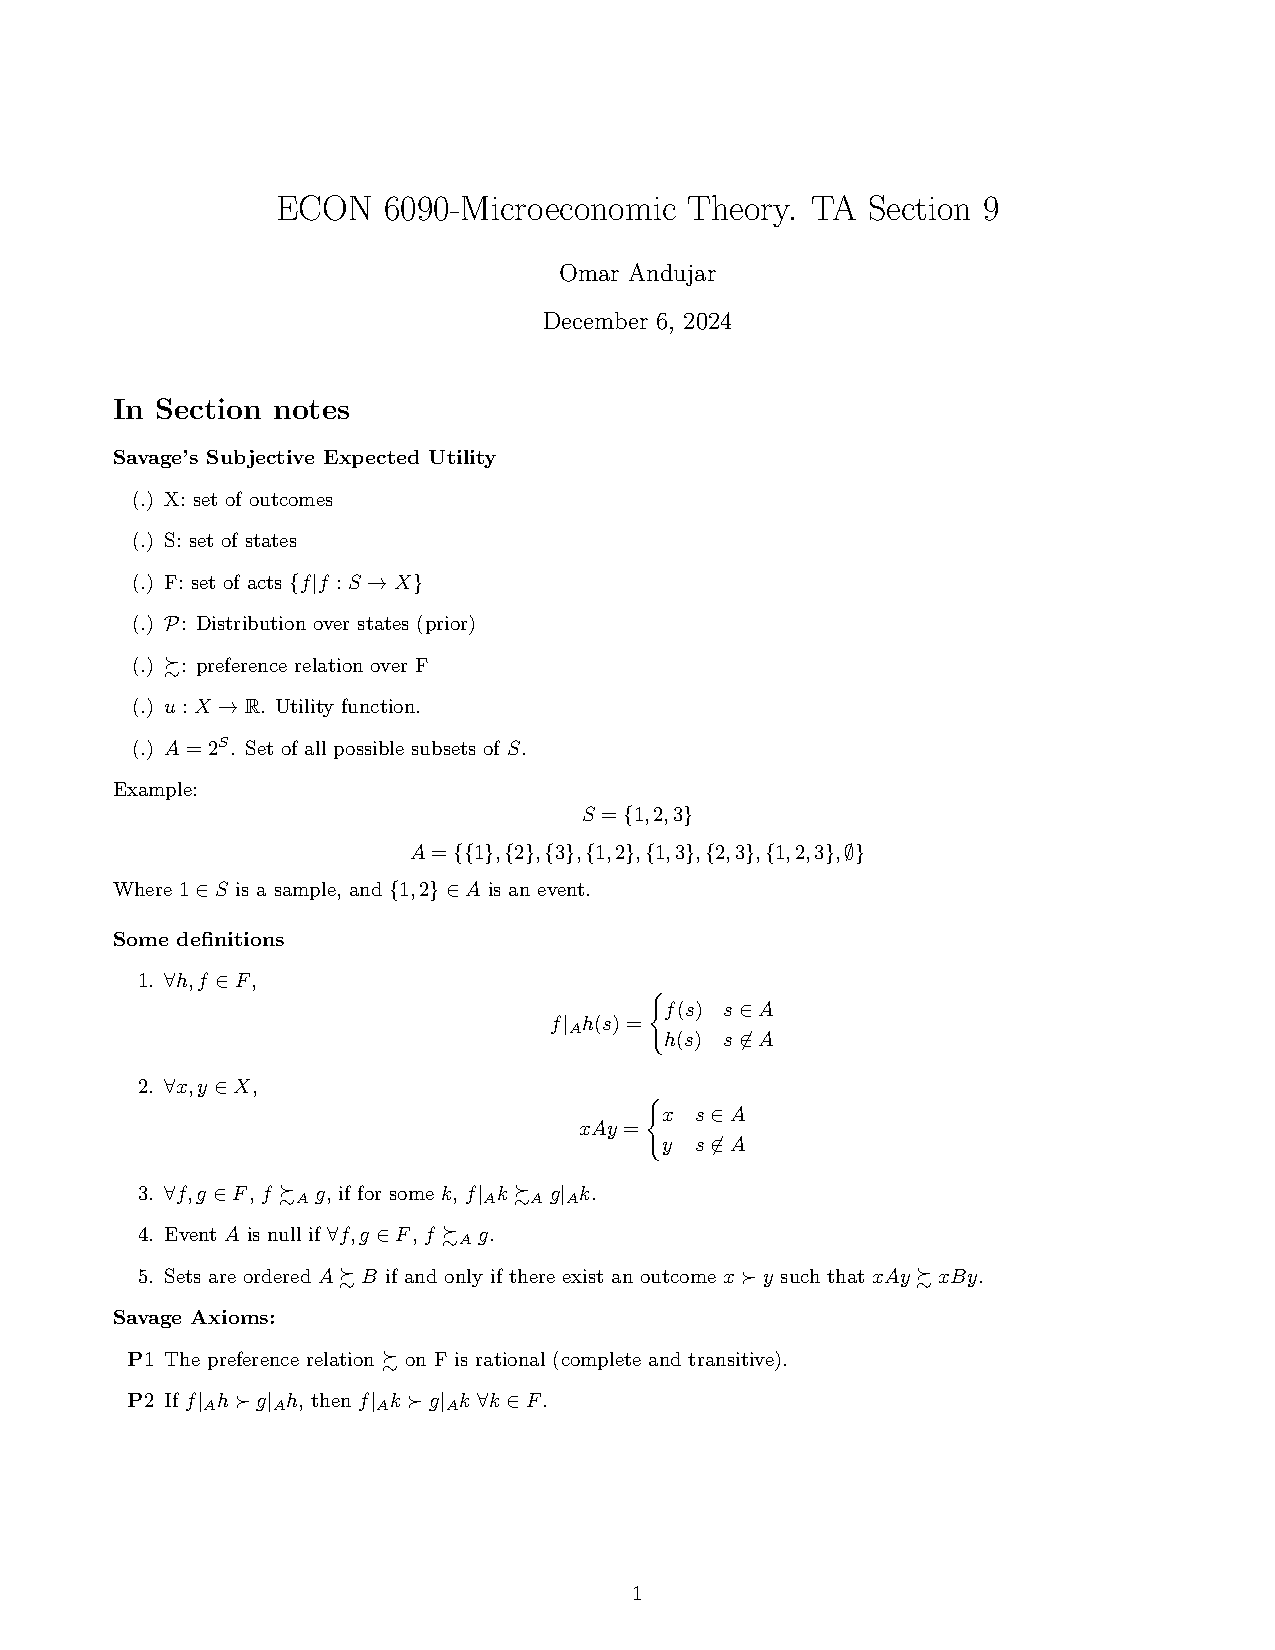
\includepdf[pages={-}]{_materials_fall_2024/ECON_6090/7._TA_Sections/Microeconomics_TASection9.pdf}

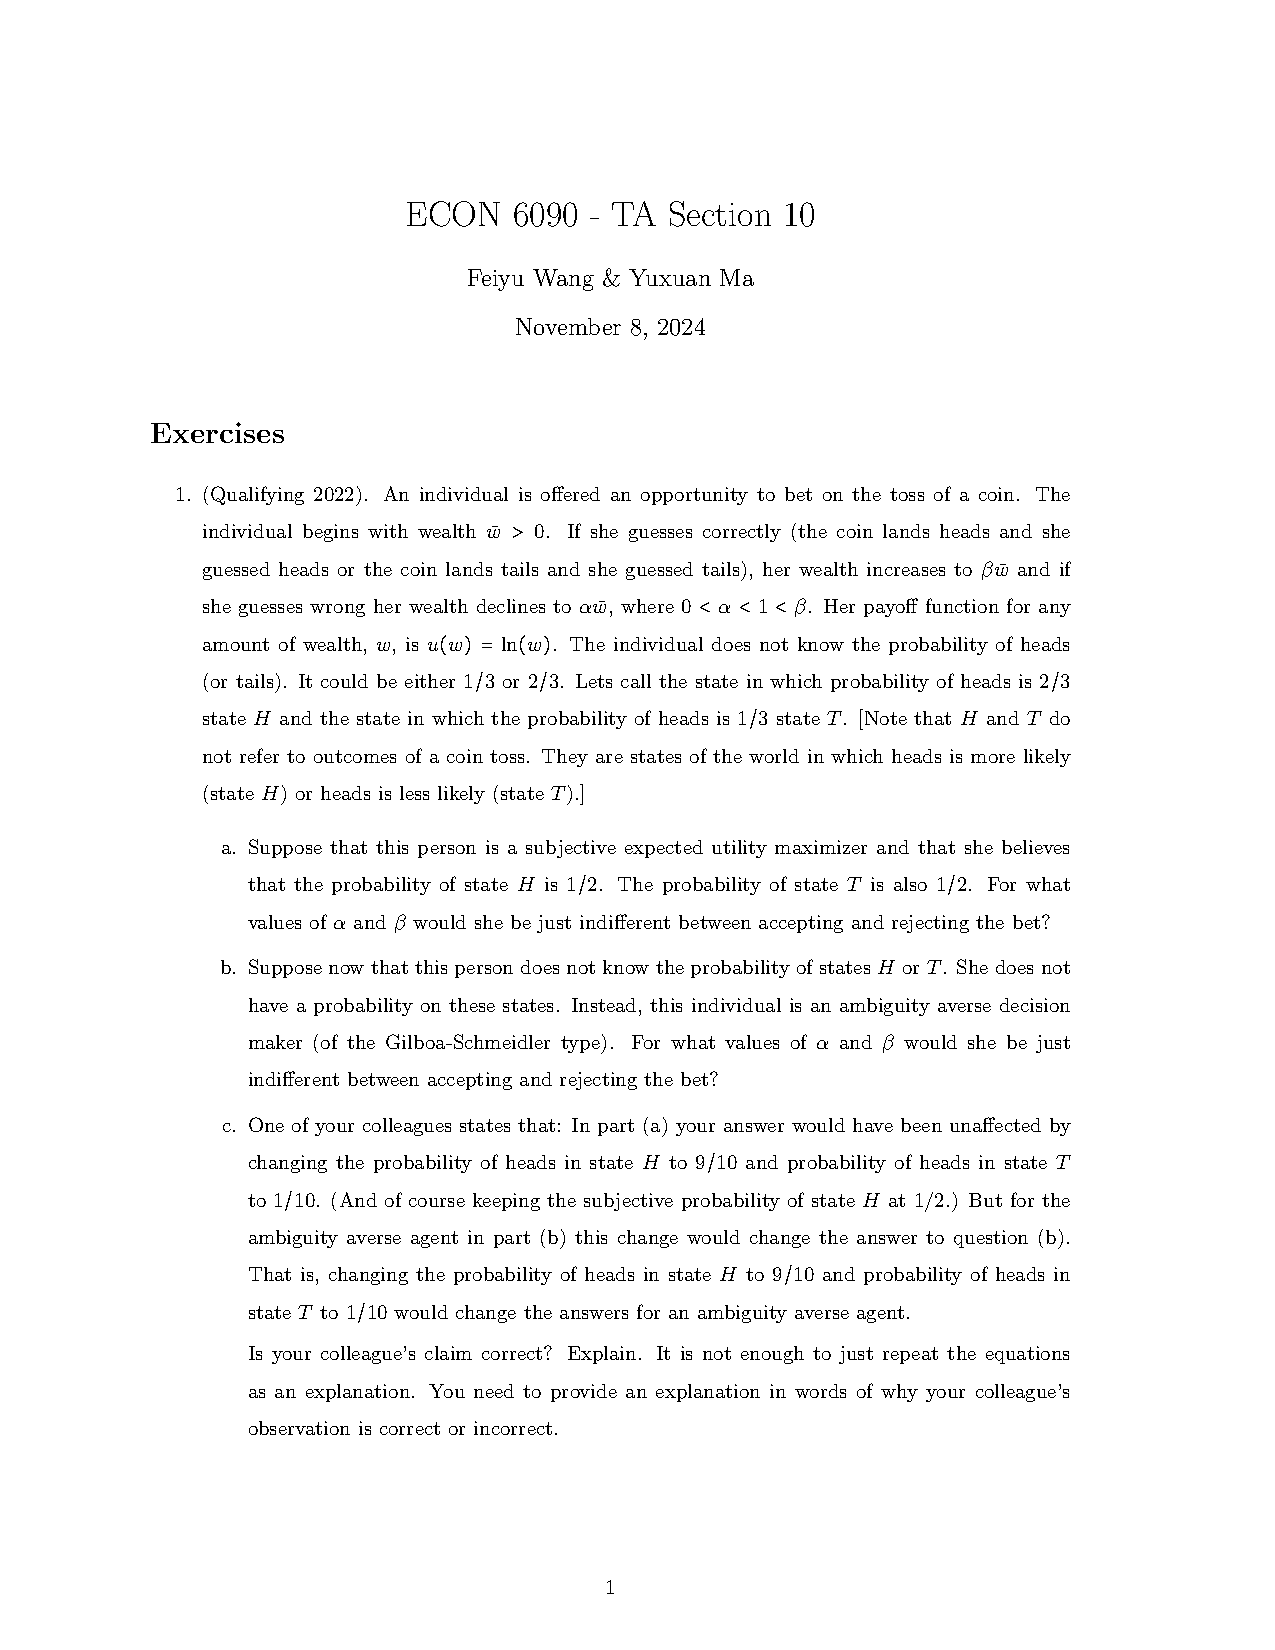
\includepdf[pages={-}]{_materials_fall_2024/ECON_6090/7._TA_Sections/ECON6090_TA_10.pdf}

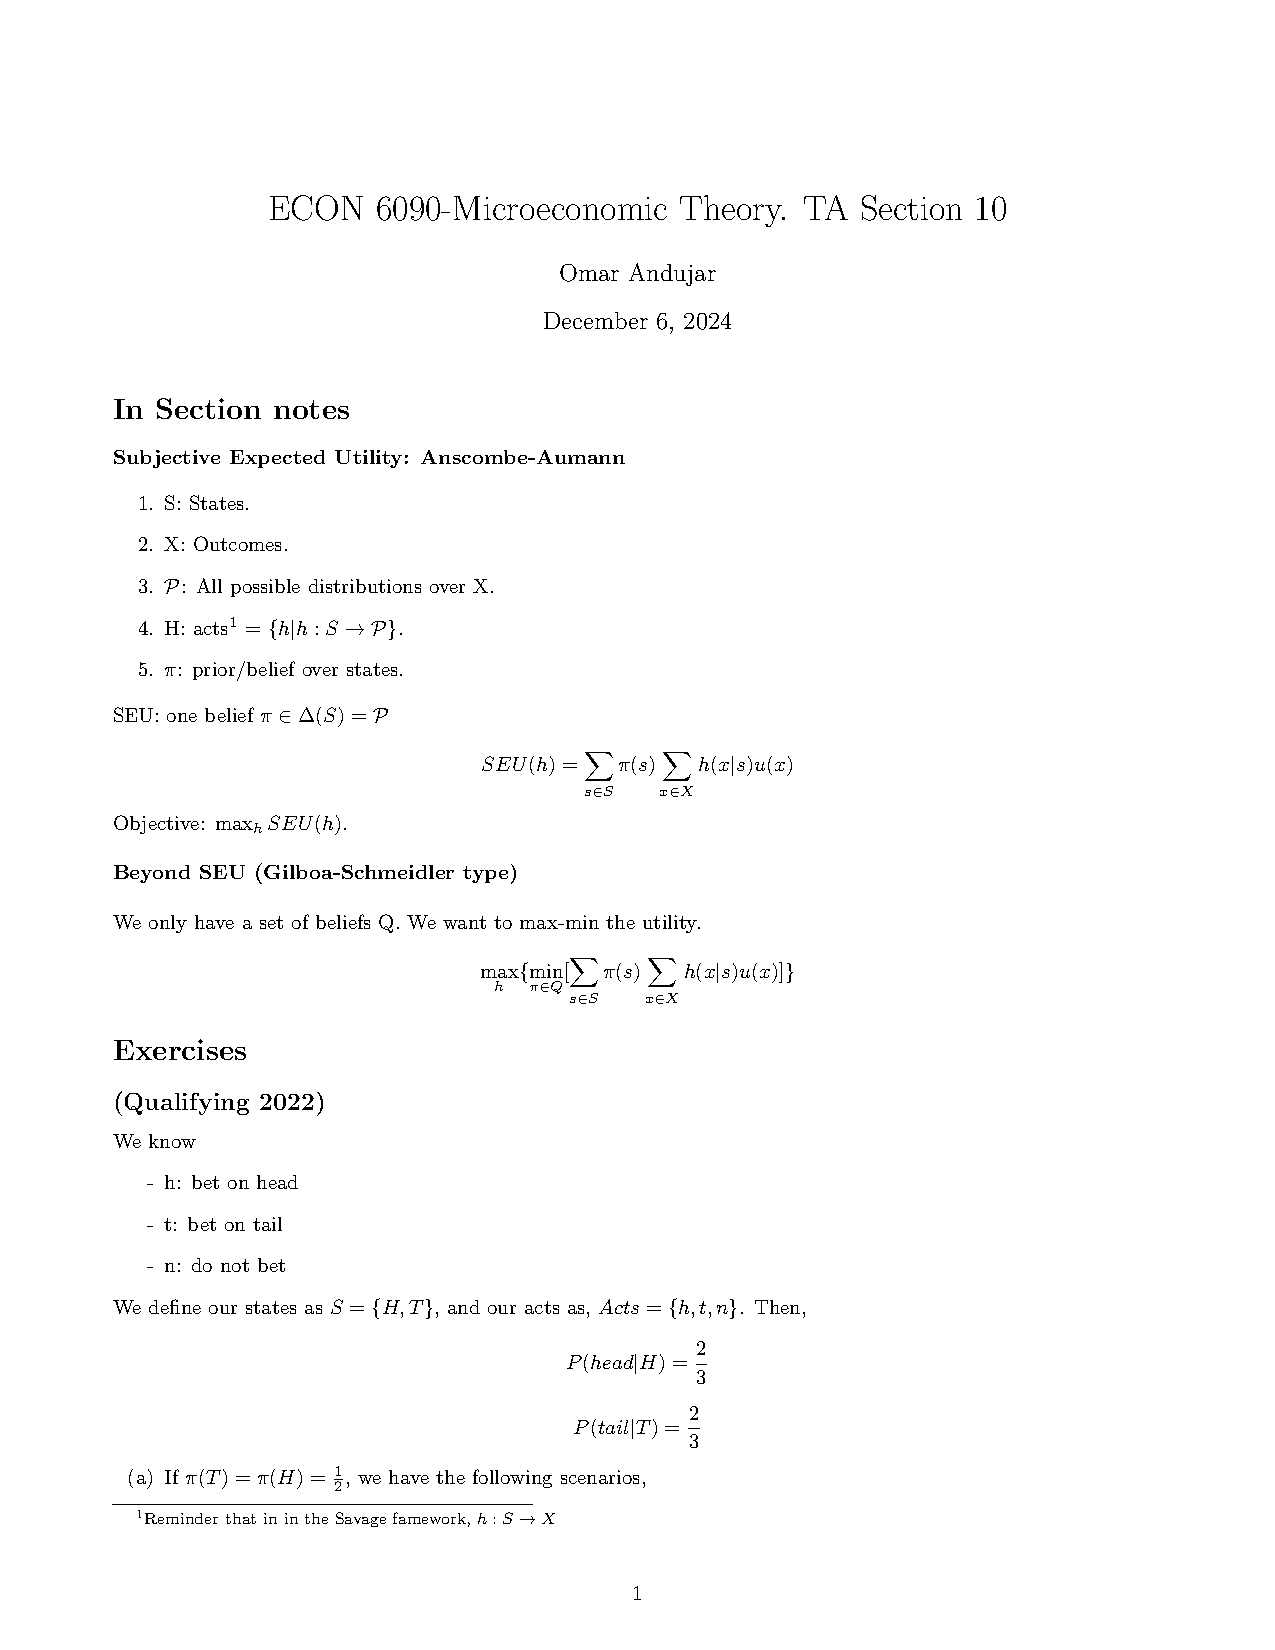
\includepdf[pages={-}]{_materials_fall_2024/ECON_6090/7._TA_Sections/Microeconomics_TASection10.pdf}


\includepdf[pages={-}]{_materials_fall_2024/ECON_6090/7._TA_Sections/ECON6090_TA_11.pdf}

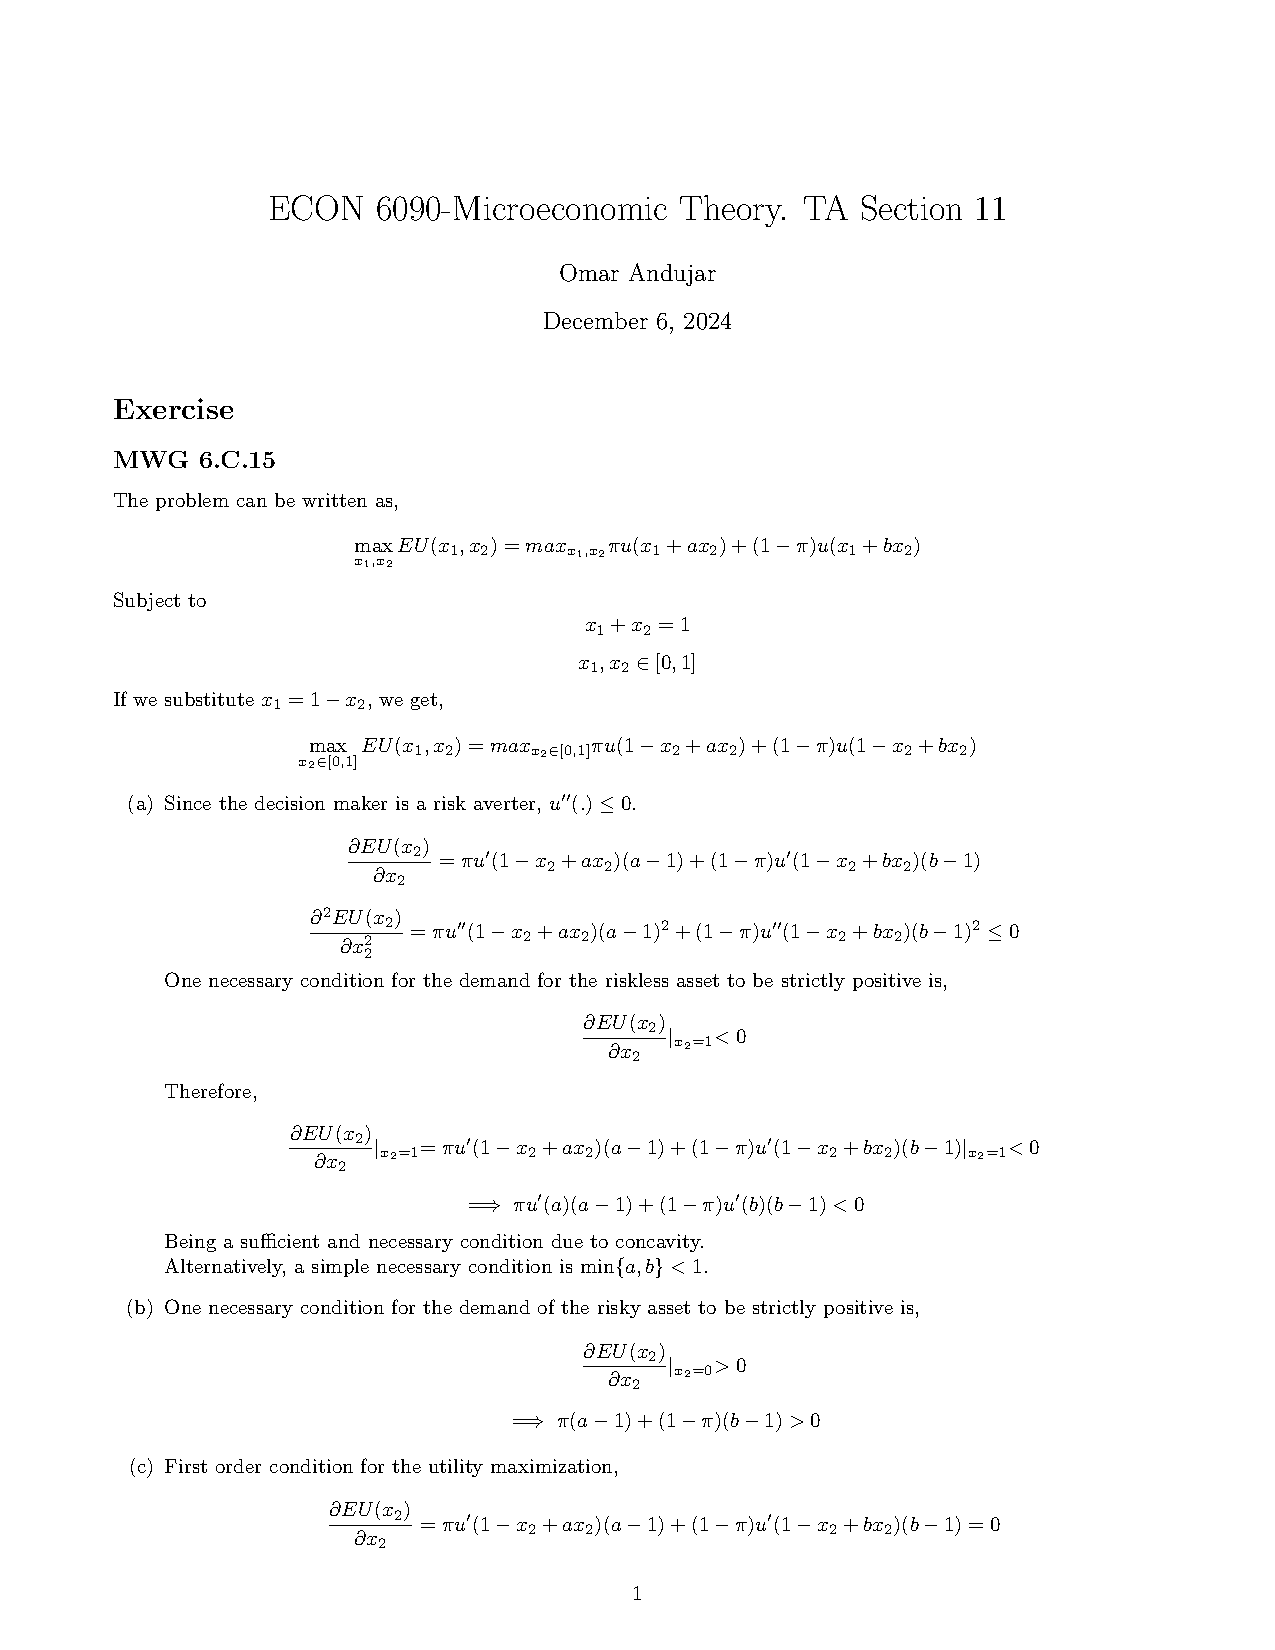
\includepdf[pages={-}]{_materials_fall_2024/ECON_6090/7._TA_Sections/Microeconomics_TASection11.pdf}



\end{document}